\documentclass[fontset=none,UTF8,zihao=5]{ctexbook}

\XeTeXgenerateactualtext=1 % 让复制文本正确

\usepackage{xpatch,etoolbox} % Hack

\usepackage{nag} % 检查过时指令

% 使用 XeLaTeX 
\usepackage[no-sscript]{xltxtra} % NOTE: 脚注在换过一种英文字体后失效,所以这里禁止改变 \textsuperscript

\usepackage{xunicode}

\usepackage{textcomp} % 扩展特殊字符

\defaultfontfeatures{Ligatures=TeX} % fontspec 使用 TeX 的语法打特殊字符





%----------------------------------------------------------------------------------------
% 将 U+2014 破折号合字 暴力修正

% via: https://github.com/CTeX-org/ctex-kit/issues/382#issuecomment-430873626

\ExplSyntaxOn
\xeCJK_new_class:n { PoZheHao }
\__xeCJK_save_CJK_class:n { PoZheHao }
\xeCJK_declare_char_class:nn { PoZheHao } { "2014 }
\seq_map_inline:Nn \g__xeCJK_class_seq
  {
    \str_if_eq:nnF {#1} { PoZheHao }
      {
        \xeCJK_copy_inter_class_toks:nnnn { PoZheHao } {#1} { FullRight } {#1}
        \xeCJK_copy_inter_class_toks:nnnn {#1} { PoZheHao } {#1} { FullRight }
      }
  }

% NOTE: 解决「。——」这种情况报错问题
% NOTE: 或者可以使用手动(正则表达式)放置空箱 `。\mbox{}——` 来解决
% 
% via: https://github.com/CTeX-org/ctex-kit/issues/382#issuecomment-491951413

\prg_set_conditional:Npnn \__xeCJK_punct_if_right:N #1 { p , T , F , TF }
  {
    \if_int_compare:w \xeCJK_token_value_class:N #1 =
                      \xeCJK_class_num:n { FullRight }
      \prg_return_true:
    \else:
      \if_int_compare:w \xeCJK_token_value_class:N #1 =
                        \xeCJK_class_num:n { PoZheHao }
        \prg_return_true:
      \else:
        \prg_return_false:
      \fi:
    \fi:
  }
\ExplSyntaxOff

% 有 0.5% 的过大误差 就先这样

% NOTE: 对 思源系字体 一定要开启特性
% 比如 `\setCJKmainfont{Noto Sans CJK SC}[Script=CJK Ideographic,Language=Chinese Simplified]`
% 或者开启 fwid 特性 `[RawFeature = +fwid]`


%----------------------------------------------------------------------------------------
%	Fonts
%----------------------------------------------------------------------------------------

% 使用 Noto CJK

% \newCJKfontfamily[notoserifcjksc]\notoserif{Noto Serif CJK SC}
% \newCJKfontfamily[sarasagothicsc]\sarasagothic{Sarasa Gothic SC}


% \newfontfamily\freesans{FreeSans}
% \newfontfamily\lmmono{lmmono10-regular.otf} % Latin Modern Mono 默认的等距字体 NOTE: 该字体不区分前后引号

% \setmainfont{Liberation Serif}[
%   UprightFont       = *,
%   ItalicFont        = * Italic,
%   BoldFont          = * Bold,
%   BoldItalicFont    = * Bold Italic,
%   Scale             = 1.1
% ]

\setmainfont{Libertinus Serif}[
  UprightFont       = *,
  ItalicFont        = * Italic,
  BoldFont          = * Semibold,
  BoldItalicFont    = * Semibold Italic,
  Scale             = 1.1
]

% \setmainfont{Linux Libertine O}[
%   UprightFont       = *,
%   ItalicFont        = * Italic,
%   BoldFont          = * Semibold,
%   BoldItalicFont    = * Semibold Italic,
%   Scale             = 1.1
% ]

% Noto Serif 可用

% FIXME: 切换成 Noto Serif 脚注不能工作 原因未知

% \setmainfont{Noto Serif}[
%   UprightFont       = * Light,
%   ItalicFont        = * Light Italic,
%   BoldFont          = * SemiBold,
%   BoldItalicFont    = * SemiBold Italic,
%   Scale             = 1.1
% ]

% \setmainfont{Source Serif Pro}[
%   UprightFont       = *,
%   ItalicFont        = * Italic,
%   BoldFont          = * Semibold,
%   BoldItalicFont    = * Semibold Italic,
%   Scale             = 1.1
% ]

% \setmainfont{Latin Modern Roman}[
%   UprightFont       = * 10 Regular,
%   ItalicFont        = * 10 Italic,
%   BoldFont          = * 10 Bold,
%   BoldItalicFont    = * 10 Bold Italic,
%   SmallCapsFont     = * Caps 10 Regular,
%   SlantedFont       = * Slanted 10 Regular,
%   Scale             = 1.1
% ]

\setsansfont{lmsans10}[
  Extension         = .otf,
  UprightFont       = *-regular,
  ItalicFont        = *-oblique,
  BoldFont          = *-bold,
  BoldItalicFont    = *-boldoblique,
  Scale             = 1.1
]

% \setsansfont{Source Sans Pro}[
%   UprightFont       = * Regular,
%   ItalicFont        = * Italic,
%   BoldFont          = * Semibold,
%   BoldItalicFont    = * Semibold Italic,
%   Scale             = 1.1
% ]


\setmonofont{lmmono}[
  Extension         = .otf,
  UprightFont       = *10-regular,
  ItalicFont        = *10-italic,
  SmallCapsFont     = *caps10-regular,
  Scale             = 1.1
]

\setCJKmainfont{Noto Serif CJK SC}[
  UprightFont       = *,
  BoldFont          = * Bold,
  ItalicFont        = FandolKai-Regular,
  Script            = CJK Ideographic,
  Language          = Chinese Simplified
]

% NOTE: FandolKai 没有 Script 选项 
% ATTENTION: FandolKai 在调用时需要与 Noto Serif CJK SC 在同一个目录下

\setCJKsansfont{Noto Sans CJK SC}[
  UprightFont       = * DemiLight,
  BoldFont          = * Medium,
  Script            = CJK Ideographic,
  Language          = Chinese Simplified
]

\setCJKmonofont{FandolFang-Regular.otf}

% via: CTeX 宏集的默认定义
% NOTE: 放在暴力修正 Fandol 字体之前

\newCJKfontfamily[zhfs]\fangsong{FandolFang-Regular.otf}
\newCJKfontfamily[zhkai]\kaishu{FandolKai-Regular.otf}
\newCJKfontfamily[zhhei]\heiti{FandolHei-Regular.otf}

% 暴力修正 FandolKai Fandol-FangSong 的基线
% via: https://github.com/clerkma/ptex-ng-dist/issues/5

% \usepackage{etoolbox} % 提供 \appto NOTE: markup-style 中已载入

\makeatletter
\newcommand*\original@CJKsymbol{}
\newcommand*\original@CJKpunctsymbol{}
\let\original@CJKsymbol\CJKsymbol
\let\original@CJKpunctsymbol\CJKpunctsymbol
\newcommand*\raise@Fandol@CJK[1]{\raise0.08\ccwd\hbox{#1}}
\appto\itshape{%
  \let\CJKsymbol\raise@Fandol@CJK
  \let\CJKpunctsymbol\raise@Fandol@CJK
}
\appto\kaishu{%
  \let\CJKsymbol\raise@Fandol@CJK
  \let\CJKpunctsymbol\raise@Fandol@CJK
}
\appto\fangsong{%
  \let\CJKsymbol\raise@Fandol@CJK
  \let\CJKpunctsymbol\raise@Fandol@CJK
}
\appto\upshape{%
  \let\CJKsymbol\original@CJKsymbol
  \let\CJKpunctsymbol\original@CJKpunctsymbol
}
% 修正包裹在 Fandol 字体中的脚注 另见 latex.ltx 6403 行
\appto\reset@font{%
  \let\CJKsymbol\original@CJKsymbol
  \let\CJKpunctsymbol\original@CJKpunctsymbol
}
\makeatother




% \usepackage{showframe} % 边框显示

% 版面设计

% 需要留出装订线距离

\raggedbottom % 向顶端对齐
\setlength{\topskip}{9.24bp} % 版心上沿到第一行基线 Adobe 系 0.88

\usepackage[b5paper,twoside, % B5 纸张 双面
hcentering, % 左右等宽
top=3.5cm, % 天高随缘
bindingoffset=7mm, % 装订线 7 mm
nomarginpar, % 暴力去除边注区域
textwidth=346.5bp, % 每行 33 个字
textheight=498.75bp % 一页 32 行
]{geometry}

%----------------------------------------------------------------------------------------
% 西文排版
%----------------------------------------------------------------------------------------

% \usepackage[english]{babel}
\usepackage{microtype} % 微排版

% 设置西文段落行距
% 参考:
% - [zhlineskip: 增加范例,单独设置西文段落的行距 · Issue #425 · CTeX-org/ctex-kit · GitHub](https://github.com/CTeX-org/ctex-kit/issues/425)
% - zhlineskip 宏包手册

\newcommand{\englinespread}{% 创建 \englinespread 标记
  \linespread{1.1} \selectfont % 西文整体行距调整 1.11 -> 1.1 调小
}

% NOTE: 使用这个会出现 headheight is too small 警告

\usepackage[bodytextleadingratio=1.5]{zhlineskip} % 正文行高修正

\newenvironment{englishpar}  % 新建「英文段落」环境
{\addvspace\medskipamount}  % 段前间距,上文段落需结束
{\par\addvspace\medskipamount} % 段后间距

\newenvironment{englishlyric}{}{}  % 新建「英文歌词」环境

% zhlineskip 宏包命令
% \SetTextEnvironmentSinglespace{1} % 根据需要修改此数,默认值是 1,适合西文「单倍」行距

\RestoreTextEnvironmentLeading{englishpar}
\RestoreTextEnvironmentLeading{englishlyric}


%----------------------------------------------------------------------------------------
% 标记的样式设定
%----------------------------------------------------------------------------------------

\newfontfamily\raintree{Raintree}[Scale=1.1] % 英文发布版带字体 注意版权问题

\newfontfamily\awesomefont{Font Awesome 5 Free Solid}[Scale=1.1] % 音乐符号

\newfontfamily\lmmonolightsmall{Latin Modern Mono Light 10 Regular}[Scale=1.1] % 拉大 1.1 倍适应中文正文
\newfontfamily\lmmonolightbig{Latin Modern Mono Light 10 Regular}[Scale=1.2] % 拉大 1.2 倍适应中文标题
\newfontfamily\lmmonocaps{Latin Modern Mono Caps 10 Regular}[Scale=1.1] % 拉大 1.2 倍适应中文

% NOTE: 废弃 仅作为 Archive
% \newcommand{\mt}{\raintree \fangsong} % mt -> mechinetalk NOTE: 另外一种样式

% mt ->  mechinetalk 需要区分中英文
% 中文:
\newcommand{\mtzh}{\lmmonolightsmall \fangsong} % \lmmonolight 1.1 倍放缩
\newcommand{\mtzhpr}[1]{{\mtzh #1}} % mtzhpr -> mtzh prefix
% 
% 英文:
\newcommand{\mten}{\raintree}
\newcommand{\mtenpr}[1]{{\mten #1}} % mtenpr -> mtzh prefix


\newcommand{\rt}{\sffamily} % rt -> radiotalk
% \newcommand{\py}{\freesans \sarasagothic} % py -> 怕音 % NOTE: 废弃 仅作为 Archive
\newcommand{\py}{\sffamily} % py -> 怕音

% \newcommand{\mtpr}[1]{{\mt #1}} % mtpr -> mechinetalk prefix % NOTE: 废弃 仅作为 Archive
\newcommand{\rtpr}[1]{{\rt #1}} % rtpr -> radiotalk prefix
\newcommand{\pypr}[1]{{\py #1}} % pypr -> py prefix
\newcommand{\rcpr}[1]{\emph{#1}} % 回忆 mrpr -> recall prefix
\newcommand{\thpr}[1]{\emph{#1}} % 心理活动 thpr -> thought prefix
\newcommand{\stpr}[1]{{\itshape \CJKunderdot{#1}}} % 强调 st -> stress % 不使用粗体 使用加点 % FIXME: 处理不优雅需要改进
\newcommand{\rspr}[1]{\emph{#1}} % 录音声音 rspr -> record sound
\newcommand{\wrpr}[1]{{\itshape #1}} % 书写 wr -> write 

%----------------------------------------------------------------------------------------
%	浮动体设置
%----------------------------------------------------------------------------------------

\usepackage{graphicx} % 插图
\graphicspath{{image/}} % 图片目录

\usepackage{float} % 用 H 选项来钉死浮动体

% 章节插图
\newcommand{\chapterintroimage}[1]{
\begin{figure}[H]
	\centering
	\includegraphics[width=0.9\linewidth]{#1}
\end{figure}
}


%----------------------------------------------------------------------------------------
%	环境标记
%----------------------------------------------------------------------------------------


% 题记样式
\newenvironment{intro}{\begin{center}\slshape}
{\end{center}\medskip}

% \newenvironment{song}{\begin{flushright}\itshape \kaishu {\awesomefont  \quad}}{\end{flushright}}

% 唱歌样式
\newenvironment{song}{\begin{flushright}\itshape}{\end{flushright}}

% 音乐样式
\newenvironment{music}{\begin{flushright}{\awesomefont\normalfont  }\hspace{\fill}\itshape}{\end{flushright}}

% \newenvironment{song}{\begin{flushright}\itshape \kaishu \marginpar[]{ \awesomefont }}{\end{flushright}}

% \newenvironment{song}{\marginpar[]{ \awesomefont }\begin{flushright}\itshape \kaishu}{\end{flushright}}


\newcommand\daytimeplace[4]{
  \begin{table}[H]
    \centering \fangsong \lmmonolightbig
    第 #1 天

    大约时间:#2

    地点:#3

    {\lmmonolightsmall {\lmmonocaps Loaction}: #4}
  \end{table}
}

\newcommand\unknowndaytimeplace{
  \begin{table}[H]
    \centering \fangsong \lmmonolightbig
    日期:N/A

    时间:N/A
    
    地点:N/A
  \end{table}
}

\newcommand\englishdaytimeplace[3]{
  \begin{table}[H]
    \centering \ttfamily
    \textsc{Day} #1

    \textsc{Time} approximately #2

    \textsc{Loaction}: #3
  \end{table}
}

\newcommand\englishunknowndaytimeplace{
  \begin{table}[H] % 钉死
    \centering
    \begin{tabular}{lr}
      \texttt{\textsc{Day}} & \texttt{N.A.} \\
      \texttt{\textsc{Time}} & \texttt{N.A.} \\
      \texttt{\textsc{Loaction}} & \texttt{N.A.} \\
    \end{tabular}    
  \end{table}
}

\font\eightssi=cmssqi8 % PostScript 字体

\newenvironment{motto}{
~\vfill
\begin{flushright}
  \eightssi \fangsong
}{\end{flushright}}

\newenvironment{note}{
\paragraph{尾注}}{\bigskip}

\newenvironment{engnote}{
\paragraph{Tailnote}}{\bigskip}

\newcommand\printstatus[7]{
\begin{flushleft}
\textbf{帕比的属性}
\end{flushleft}

\begin{itemize}
\item 力量:#1
\item 感知:#2
\item 耐力:#3
\item 魅力:#4
\item 智力:#5
\item 敏捷:#6
\item 幸运:#7
\end{itemize}
}

\newcommand\engprintstatus[7]{
\begin{flushleft}
\textbf{Puppy's S.P.E.C.I.A.L.}
\end{flushleft}

\begin{itemize}
\item{\makebox[2cm][l]{Strength:} #1}
\item{\makebox[2cm][l]{Perception:} #2}
\item{\makebox[2cm][l]{Endurance:} #3}
\item{\makebox[2cm][l]{Charisma:} #4}
\item{\makebox[2cm][l]{Intelligence:} #5}
\item{\makebox[2cm][l]{Agility:} #6}
\item{\makebox[2cm][l]{Luck:} #7}
\end{itemize}
}

%----------------------------------------------------------------------------------------
% 页眉样式
%----------------------------------------------------------------------------------------

% 在载入 geometry 之后

\usepackage{fancyhdr}

\fancypagestyle{chinese}{%
\fancyhf{} % 清空

\fancyhead[LE,RO]{\thepage}

\fancyhead[LO]{\sffamily {\leftmark}} % 奇数页  \leftmark = 章节名称
\fancyhead[RE]{\sffamily {辐射小马国:粉色双眸}} % 偶数页
}

\fancypagestyle{english}{%
\fancyhf{} % 清空

\fancyhead[LE,RO]{\thepage}

\fancyhead[LO]{\sffamily {\leftmark}} % 奇数页  \leftmark = 章节名称
\fancyhead[RE]{\sffamily \uppercase{Fallout Equestria: Pink Eyes}} % 偶数页
}

\newcommand{\fancyheadmanuallyenglish}[1]{
  \fancyhf{} % 清空

  \fancyhead[LE,RO]{\thepage}
  
  \fancyhead[LO]{\sffamily \uppercase{#1}} % 奇数页  \leftmark = 章节名称
  \fancyhead[RE]{\sffamily \uppercase{Fallout Equestria: Pink Eyes}} % 偶数页
}

\newcommand{\fancyheadmanuallychinese}[1]{
  \fancyhf{} % 清空

  \fancyhead[LE,RO]{\thepage}
  
  \fancyhead[LO]{\sffamily {#1}} % 奇数页  \leftmark = 章节名称
  \fancyhead[RE]{\sffamily {辐射小马国:粉色双眸}} % 偶数页
}

%----------------------------------------------------------------------------------------
%	分割线样式
%----------------------------------------------------------------------------------------

% 第一种样式
% \newcommand{\horizonline}{
%     \begin{center}\rule{0.5\linewidth}{\linethickness}\end{center}
% }

% 第二种样式
% \newcommand{\horizonline}{
%     \begin{center}
\includegraphics[width=0.5\linewidth]{image_line.png}\end{center}
% }

% 第三种样式 via: fancyhdr 宏包手册
\usepackage{fourier-orns}
\newcommand{\horizonline}{%
  \begin{center}
    \rule{0.2\linewidth}{\linethickness}
    \raisebox{-2.1pt}{\hspace{1em}\decofourleft\decotwo\decofourright\hspace{1em}}\,   % 然而并不对称 插入 \, 先修补一下
    \rule{0.2\linewidth}{\linethickness}
  \end{center}
}


%----------------------------------------------------------------------------------------
% 脚注样式
%----------------------------------------------------------------------------------------

% \usepackage{xpatch} % 提供 \xpatchcmd NOTE: 已在 markup-hack 中加载

% 调整脚注的分割线 via:https://github.com/muzimuzhi/latex-examples/blob/master/footnote-chinese-style.tex https://zhuanlan.zhihu.com/p/74515148

\xpatchcmd\footnoterule
  {.4\columnwidth}
  {1in}
  {}{\fail}

% ----------


\newfontfamily\footnotefont{Noto Serif CJK SC}[Script=CJK Ideographic,Language=Chinese Simplified]
% \newCJKfontfamily[footnotecjk]\footnotecjkfont{Noto Serif CJK SC}[Script=CJK Ideographic,Language=Chinese Simplified]

\newcommand{\footnotespacefix}{\hspace{-0.5\ccwd}}

\usepackage{scrextend} % 提供 \deffootnote

% NOTE: 脚注大小 7.5bp 空两个字 2\ccwd
% ATTENTION: 不要使用 em 作为单位 因为英文字体已经被放大 1.1 倍
% NOTE: 直接使用中文字体

% 样式:[1]

% \renewcommand{\thefootnote}{{\footnotefont[\arabic{footnote}]}}
% \deffootnote[0em]{0em}{2\ccwd}{{\footnotesize\thefootnotemark\hspace{\ccwd}}}

% 样式:〔1〕(最好)

\renewcommand{\thefootnote}{{\footnotefont\makexeCJKinactive\hspace{-0.5\ccwd}〔\arabic{footnote}〕\hspace{-0.5\ccwd}\makexeCJKactive}}
\deffootnote[0em]{0em}{2\ccwd}{{\footnotesize\thefootnotemark\hspace{\ccwd}}}

% 样式:[1]

% \renewcommand{\thefootnote}{{\footnotefont\makexeCJKinactive\hspace{-0.5\ccwd}[\arabic{footnote}]\hspace{-0.5\ccwd}\makexeCJKactive}}
% \deffootnote[0em]{0em}{2\ccwd}{{\footnotesize\thefootnotemark\hspace{\ccwd}}}

% FIXME: hyperref 给的方框过大
% FIXME: 需要禁止脚注换行

% 样式:带圈数字
% via: [带圈数字](https://stone-zeng.github.io/2019-02-09-circled-numbers)

% \usepackage{xunicode-addon}

% % XeLaTeX 下需要把全体带圈数字都设置成 Default 类
% \xeCJKDeclareCharClass{Default}{"24EA, "2460->"2473, "3251->"32BF}

% % 放置钩子,只让带圈字符才需更换字体

% \AtBeginUTFCommand[\textcircled]{\begingroup\footnotefont}
% \AtEndUTFCommand[\textcircled]{\endgroup}

% \renewcommand{\thefootnote}{\textcircled{\arabic{footnote}}}
% \deffootnote[0em]{0em}{2\ccwd}{\footnotesize\thefootnotemark\hspace{\ccwd}} % 需要留空


% NOTE: 以下也可行 via:https://github.com/muzimuzhi/latex-examples/blob/master/footnote-chinese-style.tex

% \makeatletter
% % add wrapper \textcircled,
% % adapted from latex.ltx, line 6380:
% \renewcommand\thefootnote{\textcircled{\@arabic\c@footnote}}

% % use separate footnote mark command
% \xpatchcmd\@makefntext
%   {\hb@xt@1.8em{\hss\@makefnmark}}
%   {\hb@xt@1.8em{\hss\@makefnmarkNormal}\space}
%   {}{\fail}

% % use non-suprescript style with lower baseline
% % adapted from latex.ltx, line 6383:
% % \def\@makefnmarkNormal{\lower .3ex \hbox{\normalfont\@thefnmark}} % NOTE: 不下调基线
% \def\@makefnmarkNormal{\hbox{\normalfont\@thefnmark}}

% \makeatother


\pagestyle{chinese} % 全篇使用 chinese 页眉样式

%----------------------------------------------------------------------------------------
%	数学相关
%----------------------------------------------------------------------------------------

\usepackage{amsmath,amssymb,amsthm}
% \usepackage{siunitx}

% NOTE: 使用统一风格的字体来表示

\newfontfamily\engfontapprox{FandolFang-Regular.otf}[Scale=1.1]

\newcommand{\engapprox}{{\engfontapprox ≈}}

%----------------------------------------------------------------------------------------
%	目录
%----------------------------------------------------------------------------------------

\setcounter{secnumdepth}{0} % 取消节编号

%----------------------------------------------------------------------------------------
%	LINKS & hyperref
%----------------------------------------------------------------------------------------

\usepackage{url}

% 强制 URL 换行 via: https://tex.stackexchange.com/questions/3033/forcing-linebreaks-in-url

\expandafter\def\expandafter\UrlBreaks\expandafter{\UrlBreaks%  save the current one
  \do\a\do\b\do\c\do\d\do\e\do\f\do\g\do\h\do\i\do\j%
  \do\k\do\l\do\m\do\n\do\o\do\p\do\q\do\r\do\s\do\t%
  \do\u\do\v\do\w\do\x\do\y\do\z\do\A\do\B\do\C\do\D%
  \do\E\do\F\do\G\do\H\do\I\do\J\do\K\do\L\do\M\do\N%
  \do\O\do\P\do\Q\do\R\do\S\do\T\do\U\do\V\do\W\do\X%
  \do\Y\do\Z}



\usepackage[xetex]{hyperref}

\hypersetup{breaklinks=true,
            pdfauthor={RandomQuantum},
            pdftitle={Fallout Equestria: Pink Eyes 辐射小马国:粉色双眸},
            pdfcreator={XeLaTeX with CTeX and hyperref},
            pdfkeywords={FoE}
            }

%----------------------------------------------------------------------------------------
% 目录问题解决
%----------------------------------------------------------------------------------------

% NOTE: 需要放在 hyperref 后面
% 规定 chapter 的计数器的上级为 part,使得每个 part 后 chapter 清零
% 暴力使用 setcounter{chapter}{0} 会使得 hyperref 错误
\makeatletter
\@addtoreset{chapter}{part}
\makeatother
% via: [sectioning - How to reset chapter and section counter with \part - TeX - LaTeX Stack Exchange](https://tex.stackexchange.com/questions/54383/how-to-reset-chapter-and-section-counter-with-part)







\title{Fallout Equestria \\ 辐射小马国 \bigskip \\ {\Large Pink Eyes \\ 粉色双眸}}
\author{Mimezinga \and MadCatMKII}
\date{}


\begin{document}

\frontmatter % 前言开始

% \layout % 版面查看

\begin{titlepage}
    
\begin{center}


{\huge \bfseries
Fallout Equestria \medskip \\ 辐射小马国
}

\bigskip

{\LARGE \bfseries
Pink Eyes \medskip \\ 粉色双眸
}

\vspace{6em}

Mimezinga \quad MadCatMKII

\vfill

{\scshape Community Release}


\end{center}

\end{titlepage}


\newpage

~\vfill

\thispagestyle{empty}

\begin{englishpar}
\noindent This is a work of fiction. Names, places, and incidents either are the product of the author's imagination or are used fictitiously. Any resemblance to actual ponies, living or dead, events, or locales is entirely coincidental.
\end{englishpar}

\noindent 这是一部虚构的小说。本作品中的部分角色和地点名称选取自孩之宝公司的影视作品《小马宝莉:友谊是魔法》(\emph{My Little Pony: Friendship is Magic}),除此之外本作品涉及的名称以及地点和事件要么是作者想象的产物,要么是虚构的。与实际的小马,生活或死亡,事件或地点的任何相似之处均为巧合。\\

\begin{englishpar}
\noindent Article and OCs \textcopyright\ Mimezinga

\noindent \emph{My Little Pony: Friendship is Magic} \textcopyright\ Hasbro, Inc.

\noindent \emph{Fallout} \textcopyright\ Bethesda Softworks, LLC

\noindent \emph{Fallout: Equestria} \textcopyright\ Kkat

\noindent Cover \textcopyright\ LimreiArt

\noindent Illustrations \textcopyright\ Boiler3 \\

\noindent \textsc{Self-Released}\\
\end{englishpar}

\begin{englishpar}
\noindent This work references characters and locations that are copyright and trademarks of Hasbro, Inc. No claim is made on Hasbro's copyright or trademarks.
\end{englishpar}

\noindent 本作品仅可用于个人欣赏和学习交流之用。任何人不得以任何形式将本作品用于商业用途,否则一切后果自负。\\

\begin{englishpar}
\noindent This book is powered by \XeLaTeX{} and \CTeX{}
\end{englishpar}


\chapter{简介}

小马国52号公路,也就是52号国道,正在渐渐衰败着。从盐块城到翡翠海岸的那一段,一座座城市变成了空城,几年前商旅队还能安全穿行的地方现在游荡着奴隶贩子和强盗。北边的山岳里神秘的生物若隐若现,沙漠似乎在吞噬着哪怕是装备最齐全的探险队。以前埋下的祸根此时正纷纷破土而出,但没有小马愿意拯救这一切。

是时候迎来我们的英雄了。

\clearpage

\begin{motto}
你相信幽灵吗?
\end{motto}



\chapter{排版者前言}

\section*{原版中译前言}

首先,感谢《辐射小马国:粉色双眸》作者 Mimezinga 带给我们的精彩故事,感谢《辐射小马国》作者 Kkat 打造的庞大世界观,也感谢所有直接或间接参与制作的朋友,没有大家的努力,不会有现在的成果。

其次,由于译文与原文之间不可避免的差异,无法完全翻译出原著小说的意境,推荐有条件的朋友阅读原著。

然后,尽管我们很努力想要排查本作品中存在的文字、语法以及标点符号错误,但由于文章篇幅较大,难以做到百分之百的正确率,请谅解。

最后,由于目前没有申请 ISBN,该作品无法正式出版,想要收藏实体书的朋友需要以自愿的原则自行打印。笔者不会出售相关实体书籍,也不会以任何形式收取任何费用,更不会授权任何人使用本作品进行商业活动。如果您发现有人贩卖基于本作品的相关产品,请谨慎小心,以防上当受骗。

\begin{flushright}
ShadowDumb

2019 年 5 月 29 日
\end{flushright}

\clearpage

\section*{\LaTeX{} 重排版前言}

采用 \LaTeX{} 重新排版;英中双语版本;对原版进行初步排版校准,使之符合印刷排版标准;修改书籍结构;并改正部分中译版字句错误(例如大小写错误、空格错误、译文错误)。

此版本仅有中译版。

\begin{flushright}
RandomQuantum

2019 年 6 月 15 日
\end{flushright}


\begin{motto}
「战争,战争从未改变。」

\medskip

「小马……小马从未改变。」
\end{motto}



\tableofcontents

\mainmatter

\chapter{避风港}

\chapterintroimage{image01.png}

\begin{intro}
    你相信幽灵吗?
\end{intro}

「拜托让我们上车!防护罩要失效了!快没时间了!」

长长的一大队小马焦急地等在一辆天空马车前,但是却没有看到拉车天马出现。忽然队末的一只绿色独角兽雌驹疯狂地推着马群尖叫起来。

「这不可能!这不可能!怎么可能会这样!?赛拉丝蒂亚抛弃了我们!露娜抛弃了我们!这……」

砰!

慌乱的雌驹无声地倒在了地上,所有小马齐刷刷转头看过去,卫兵正在将子弹压入霰弹枪。

「整整齐齐站成一排!排好队挨个上车!谁找麻烦我只好用致命手段了!」

中心城的塔楼之下穿行着惊慌而绝望的马群,它们将成为这场歇斯底里的疯狂毁灭行为的见证者。

\horizonline

远处上方中心城的街道上,小马们发疯一般争先恐后地寻找庇护。整个街区都被大火吞噬,许多道路都被翻倒的马车、破碎的建筑物和一些残垣断壁堵住了。但还有一些小马试图互相帮助,努力清理道路并救助伤马。

在一条拥挤的街道上,一群种马试图破开一堵残损的墙。

「再来!大家一起!使劲儿!」小马们再次用力向墙上尥去,爆发出自己全身的力量。

终于,墙屈服了,塌出了一个大家都能通过的缺口。除了一只年轻的小雌驹不知道发生了什么以外,这条路已经空了。她坐在街道中间,眼睛盯着她的鬃毛,接着又盯着天空。远处,一个巨大而闪亮的泡泡包裹着整个城市。在她盯着泡泡看的时候,有些东西击中了护盾的顶部并爆发绚丽的光芒。

「哦,耶!烟花!」她高兴地喊了出来。

「嘿,那边的小鬼!」

一个穿着白色制服的独角兽医疗兵正在给幼驹发放防护服。在看到这只小雌驹的时候,她冲了过去,露出了令马担忧的表情。

「就你自己吗?你家长哪儿去了?」

幼驹对着医官微笑着。「妈妈在那上面!」她用蹄子指着中心城的闪光防护罩,防护罩现在看起来比10分钟之前薄了很多。「她晚餐的时候就会回来!」

士官踌躇了一下,然后对幼驹勉强一笑。「当然……她会回来的。小家伙你叫什么名字?」

「我叫快乐帕比(Puppysmiles)!」幼驹开心地蹦蹦跳跳着。

「好的……好的……帕比,没关系……你仔细听好,穿好这件外套,不管发生什么事情,都不要脱下来,好吗?」

幼驹有些疑惑的视线在黄色的东西和白制服独角兽之间来回转了转,「好的,漂亮的大姐姐!我喜欢你!」

独角兽紧张地笑了笑,然后漂起并展开了防辐射服:那是一件柠檬黄色外套,蹄子上有几个口袋,体侧还各有一个鞍包。

「好,你要把你的蹄子放进这些洞洞里面,就像是……像是……小马舞一样!你知道小马舞吗?」

「当然!」

% NOTE: 遵照英文发布版改

\begin{song}
    「右蹄伸出去
    
    右蹄缩回来!」
\end{song}

「对对,就是这样!然后是尾巴……好了,然后让我给你密封好,最后是把这个放在你的头上……好了!」

雌驹把一个原型的玻璃头盔戴在了帕比头上,然后把两边的卡扣锁紧,把孩子安全地包在了她的防辐射服里面。

「哇塞!我看起来就像是个太空小马!就像是……像是安德洛队长一样!呜!!!」幼驹兴奋地蹦来蹦去,白色的雌驹微微松了口气,然后转头走向下一队幼驹。

快乐帕比觉得现在真开心极了。一个巨大无比的烟花爆炸了,它听起来像一个非常棒的派对礼花!城堡被超大的肥皂泡泡包着,就像是妈妈用肥皂吹出来的那样,不过要大很多很多。大家都像在大庆典之前一样走上了街头。她偷偷对自己的幸运星祈祷妈妈能够早点回家,这样今天她就能和妈妈早点在一起玩耍了。而这个超级酷的太空服更是大大的意外惊喜,看来大家都想把她打扮得漂漂亮亮的,然后……对了!现在她需要面镜子!小雌幼驹毫不犹豫地跑回家去。

\horizonline

在她妈妈的卧室里面依稀听得见街上喧闹的声音,帕比站在梳妆台之前,仔细看着她的头盔,她面前出现好多奇怪的发光符号和文字。不管她看向什么那东西就会被一层奇怪的绿光笼罩,然后下面出现一些小字……可惜的是帕比认识的字不多,她妈妈还没怎么教她。

「嗯……唔……这个字是……」幼驹皱着眉头看着那个字,「床!哇哦,我好厉害!」

帕比得意洋洋地走下楼,完全把镜子的事情忘在脑后,转身打开了冰箱。

「马芬!」

帕比拿起托盘正准备咬,但是却发现一个问题——她带着这个笨头盔根本吃不到……{}

「好麻烦……坏头盔!我该怎么把你拿下来?」她用双蹄抱着那个倒扣在自己头上的鱼缸用力扯了好几分钟,但是那东西纹丝不动。她气喘吁吁地坐下来,然后祭出了她的王牌。

「哇啊啊……」

大哭的时候帕比没注意到,一个红色的符号出现在视野下方。但是她的哭声被这件外衣的奇怪机械声音打断了。

「{\mtzh 主体状态——恐慌!}」

幼驹傻傻地眨了眨眼睛,发生什么了?谁在说话?

「唔?」

「{\mtzh 开始内部医疗检测。错误。系统重启。请等待……30秒。}」

这些话很有趣,但是对于帮她脱掉头盔却一点用也没有。帕比依然很不开心。

「走开,笨笨说话衣服!我要吃马芬!」

「{\mtzh 重启完成。检测版本。开始……十秒钟后检测结束……八……七……}」

在那一瞬间,外面的噪音变得更大——空气中从充满了尖叫声和哭喊声。帕皮觉得可能是外面的小马在唱歌。

「{\mtzh 五……四……三……}」

忽然整个世界都变成了粉色。幼驹可以看到窗外似乎有一个巨大的黑影降落在城市上空,就好像一个巨大的粉色棉花糖云从天而降,它似乎在一瞬间便吞没了街道,房屋和所有的小马。完全不知道发生了什么的帕比紧贴着玻璃窗,很好奇窗外有什么异变。

「{\mtzh 二……一……系统重启完成。开始自检。警告,主医疗护符\footnote{主医疗护符(Talisman):辐射小马国(Fallout Equestria)中设定的一种可以施展固定法术的的蚀刻符文。}没有响应。启动备用医疗护符。开始诊断。雌性,幼驹,陆马族。}」

哇哦,这个太空服真聪明!他知道的可真多!

「嗨,我叫快乐帕比!」

粉色的浓雾像毯子一般整个覆盖在了街道上,模糊不清的尖叫声变成了咳嗽声,小马的声音随着云将他们杀死或者变成更糟糕的东西而渐渐变弱。

\mtzhpr{「生命维持系统上线,体温正常,血压正常。警告,辐射水平超过正常水平300\%。」}

帕比咯咯地笑着:「咦嘻,太空服先生在说些听不懂的话!」帕比茫然地站在窗前看着正在漏进屋内的奇怪粉雾。她不知道……{}

\mtzhpr{「警告。检测到小量辐射毒性。注射:抗辐剂\footnote{抗辐剂(Rad-X):增加辐射抵抗能力。},注射:辐特宁\footnote{辐特宁(Rad Away):清除体内辐射。},注射:辐……」}

\mtzhpr{「 警告,危险药剂侦测,分析中。粉色药剂,幼角型\footnote{幼角型:Littlehorn type,或者下文的 Littlehorn agent 都是 \emph{FoE}(\emph{Fallout: Equestria})中粉雾(Pink Cloud)的「小马国官方」说法。}。浓度超过5\%可能致命。」}

「{\mtzh 1.8\%……2.0\%……2.2\%……警告,粉色药剂超过安全上限,建议立刻离开该区域。}」

帕比盯着地面上弥漫在蹄子间的粉色迷雾,看起来就像是棉花糖……粉色的棉花糖!

耶!自从上次噩梦节(Nightmare Night)她吃棉花糖吃到吐之后,她妈妈就再也没让她吃过。

% NOTE: 漏译,补上

突然,她感觉肚子收缩了一下。

「我觉得好好玩……」

「{\mtzh 危险!检测到变异产生!浓度达到 5.4\%。危险!6.0\%!请立刻离开!请立刻联系和平部\footnote{和平部(Ministry of Peace):小蝶创建的部门,主要负责健康事务和医疗方面的研究。} 获得救治!开始发送求救信号。扫描应急信道。发送中。警告,浓度达到 7.5\%}」

「呃……妈妈……我觉得……不太舒服……明天可以……请病……」幼驹面前的一
切都变得雾蒙蒙的,她觉得自己出了好多汗,但是又冷得像掉进了冰窖。

「{\mtzh 注射:治疗针(Med X),注射:治疗药水\footnote{治疗药水(Healing potion):\emph{FoE} 设定里的一种魔法药水,可以治疗大多数轻度伤病。}。浓度达到 12.1\%。注射:抗辐射药,注射:辐特宁。检测到粉色药剂浓度达到 16.0\%。注射:解毒药,注射:治疗药水,注射:治疗药水。浓度达到 22.6\%。注射:治疗药水,注射……}」

冗长枯燥的防辐射服医疗系统声音不断地重复着,一直到帕比的四蹄再也支撑不住自己,她失去意识,倒在了厨房地板上。充满她静脉的治疗药只是勉强延长着她的生命,致命的粉色药剂云雾正慢慢吞噬着防辐射衣,而医疗系统正在竭尽全力保证幼驹的性命,她还没有死,但是却不可能活下去。

「{\mtzh ……治疗药水,注射:治疗药水,注射:治疗药水,注射:治疗药水。警告,治疗药水剩余:3。检测到粉色药剂浓度达到 35.0\%。注射……}」

帕比就像一个被遗弃的玩偶那样躺在那里,衣服的声音还在不断报告着危险气体地渗入。最后衣服也放弃了,因为医疗药品已经耗尽。她再也没有听到那个声音。一个小时,两个小时,一天,两天……

幼驹只是躺在那里,穿着一件聒噪且唠叨不停的防护服,它只是在不停地提醒着幼驹她几乎要死了,而她需要……所有东西才能救她。

一天天过去,一周周过去,一月月过去。帕比还是那样安静地睡着,静止在她生命中的最后一刻。

几个月变成几个季度,几个季度变成几年,衣服还是不停地唱着它的摇篮曲。

几十年过去了,衣服的声音也越来越低,开始沙沙作响,被尘土覆盖的透明头盔好像是为睡个长长午觉的幼驹拉上安眠的窗帘。雌驹尘封在小小衣服中,被厚厚云雾笼罩,几十年慢慢变成一个世纪……两个世纪……

年久失修的房子开始慢慢风化,这是一栋非常坚固的房子,由陆马用传统办法一砖一瓦盖起来的。但是任何东西都有它的寿命,它开始因为春雨洗刷屋顶而发生裂痕,而夏天的每一场暴风雨侵袭,都让这小小的裂痕在慢慢变大。终于整幢屋子寿终正寝倒了下来。

正好砸在了小小快乐帕比的头上。

\horizonline

\daytimeplace{1}{5:00 PM}{四叶天台,中心城郊区}{Clover Leaf Terrace, suburb of Canterlot}

当坍塌的屋子消失在一片尘土和粉色烟雾之中,一切又重新回归了寂静。尘埃慢慢落下,在废墟之下却冒出了一个含糊不清的小小声音。

「好痛哦……」

慢慢地,一块砖动了动,然后是另一块,在碎石之中冒出一个闪闪发光的东西,一个圆圆的玻璃球头盔冒了出来,然后是一个穿着黄色防辐射服的小小身影。那头盔上有一道长长的裂痕,但是当幼驹从倒下的房子里爬出来的时候,那个裂痕就神奇地消失了。

「妈咪?」幼驹就像是一个踏上未知星球的宇航员一样。「这是哪里?大家都去哪了?妈咪?妈咪……?」

好像有什么不对劲的地方,她觉得自己还穿着那个会讲话的衣服。

「妈……咪……!」

「{\mtzh 兹兹……沙沙……线路……必须……重启……}」

「安静啦衣服!妈妈去哪了?房子去哪了?我到底……」幼驹抬头的时候把下半句憋了回去,因为在山顶之上的城堡废墟,是她绝对不会认错的中心城——她的故乡。

「什么……怎么……怎么坏成那样!」

「{\mtzh 吱吱……严重错误……没有组件……区需要去去去……启启起起起起……}」

「好吧,随你吧!」幼驹叫着,她看着头上中心城的废墟。忽然那种奇怪的感觉又来了。最初是她的视线变得模糊不清,然后她一屁股坐在了地上,她的蹄子都站不稳了,她觉得越来越虚弱,有一股剧痛穿过她的脊椎。那是一种奇怪的感觉,她的全身好像都停止工作,小幼驹想要大声尖叫,但是嘴都动不了。她唯一能做的事情就是在剧痛之中透过满是灰尘的头盔看着街道。

她只能坐在那里,看着一堆奇怪的灰白色肮脏石块,有大有小,有直有弯。现在她才注意到那些东西到处都是,不过很快一个绿点闪过她眼前,引起了她的注意。

「{\mtzh 系统重启完成。检查版本。未找到文件。启动应急模式。版本0.2……}」

帕比想说点什么,但是她还是完全麻痹,幼驹只是盯着眼前的那些奇怪的光点由绿色变为了粉色。嘿,终于有点儿好消息了,至少,她喜欢粉色!

「{\mtzh 发现新硬件。初始化矩阵。连接中。}」

火花穿过了幼驹的整个身体,从鼻尖到尾巴尖,冲走了全部麻痹的感觉,幼驹有些迟疑地举起一只蹄子,发现完全没有难度。然后她又走了两步,没有问题!就好像5分钟前的事情完全没发生一样,一瞬间医好了。

「哇哦,真奇怪……现在我只要把这个笨笨的太空服脱掉……」

「{\mtzh 全系统正常运作。开始例行监测。分析中。目标001,快乐帕比,雌性,幼驹,陆马种族。未发现内脏。检查系统错误,未发现错误。继续进行检查,雌性,幼驹,陆马族,无内脏。}」

「吴奶藏是什么?我想要!好吃么?」

「{\mtzh 读取幼驹学习程序。连接到印象部\footnote{印象部(Ministry of Image):瑞瑞在大战时创建的部门,负责形象设计与战时宣传。}。寻找最新版本。无法建立连接。从备份文件读取,请等待安装完成。}」

幼驹开始晃来晃去,在那堆风化的石头上走来走去,想挨个看看它们。头盔的抬头显示屏(HUD)把整堆白色的石头都用粉色的光晕包裹起来,下面的显示文字甚至还有拼音。

「似……是……尸……体?尸体!」幼驹开心的晃着,她最喜欢读拼音了!然后她又皱起了眉头。

「尸体是什么?」

「{\mtzh 尸体,名词,死亡生物的残骸——就这样!}」机械的声音快速地回答了问题。

「死亡?就是那个……死亡的死亡?」

「{\mtzh 寻找死亡的同义词……逝世,牺牲,灭亡,丧生,归天,凋落,断命,升天,毙命,枯萎,陨命,殒命,仙逝,弃世,死灭,亡故,去世,去逝,物化,仙游,作古,衰亡……}」

帕比听着长长列表的一小段就没了兴趣,然后用一只蹄子戳着一块长长的骨头,她因为注意到骷髅之中熟悉的东西而睁大了眼睛。

「呃……声音先生……这个尸体……是什么?」

「{\mtzh 分析中……小马。成年雌性。独角兽族。}」

小小幼驹打了一个寒噤,或者至少她觉得自己打了一个寒噤,她抬起头来看着街上到处都是的骨头。骨架有的独自蜷缩在角落,还有的几个抱成一团好像觉得马多就会安全。都已经死了,所有马都死了。

「发……发生了什么?妈咪?妈妈哪里去了?」帕比觉得浑身冰凉,「声音先生……妈妈去哪了?」

「{\mtzh MoM,士气部\footnote{士气部(Ministry of Morale):战时萍琪派创建的部门,主要负责鼓舞士气,后面缩写为MoM。},分析数据,连接小马国地图数据库。下载数据,错误,没有相似数据。寻找 MoM 广播信号。发现机器精灵\footnote{机器精灵(Spritebot):萍琪派制造的一种悬浮机器人,类似 \emph{FO: NV} 中的 EDE。},建立数据连接……}」

快乐帕比从第一句话开始就听不懂在说什么了,现在她正在找自己的家,或许妈妈在家里等她呢。

「为什么完全不一样了,我的房子哪去了?其他漂漂小马都在哪儿?」

顺着荒芜的街道,她看到了甜圈乔的商店,于是才确定这是自己居住的街道,而她家一定在……「但……但是……」她站在她几分钟之前爬出来的废墟面前,一脸地难以置信。

「{\mtzh 发现广播信号源,正在进行地标信息传送……}」

「如果这是我家……妈妈呢?」帕比坐下来开始哭,或者至少试着要哭。很快她发现自己只是在发出声音,没有眼泪从脸上滑落,而且她一点都没有感觉到宽慰。现在幼驹觉得她自己一定有什么不对,她正打算问那个声音,但是却被打断了。

「{\mtzh 士气部地点已经添加到地图。最近的 MoM 分部作为导航终点。}」

「你……找到妈妈了?」帕比惊呼,感到一阵希望。

「{\mtzh 肯定。MoM 已经定位,中心城外最近的 MoM 分部已经设定为目标地点。}」

「呃……我……我想那就是找到了?」小家伙歪着头。

「{\mtzh 说明:请按照罗盘上的粉红色箭头前行,直到到达目的地。}」

「呃……谢谢?」幼驹花了几秒钟才意识到这是多么棒的事情。这个声音刚刚找到她的妈妈了!她马上就能见到妈咪,然后就没事了!谁还管房子,死掉的小马,变成废墟的城堡还有那笨蛋……等等,反正这个超超超超超级聪明的说话太空服要带她找妈妈,让帕比感觉到无比的开心和宽慰。谁还管她为什么不觉得饿或者累,妈妈会知道为什么!她只要找到妈妈,不管什么问题都不是问题!

「耶!」

\horizonline

\daytimeplace{1}{8:30 PM}{阳光广场,中心城外}{Sunshine Plaza, outskirts of Canterlot}

「{\mtzh 警告,缺少重要生命指标。警告,医疗补给耗尽。警告,所有紧急频道没有响应。警告……}」

\begin{song}
「警告扫除!警告扫除!」

\begin{englishlyric}
    ``Warning wrap up warning wrap uuup!''    
\end{englishlyric}
\end{song}

帕比一边在中心城外的大街上溜达着,一边唱着自己版本的冬季扫除,她想要和衣服的声音合起来变成重唱,但是看起来没那么容易。

\begin{song}
「医疗补给已经累了!

\begin{englishlyric}
    ``The medical supply's tired!
\end{englishlyric}

\medskip

警告扫除!警告扫除!

\begin{englishlyric}
    Warning wrap up warning wrap up!
\end{englishlyric}

\medskip

我们马上还需要电池!」

\begin{englishlyric}
    We'll soon need batteries!''
\end{englishlyric}
\end{song}

「{\mtzh 否定。能源存量足够。魔能火花\footnote{魔能火花(The Spark):\emph{FoE} 中虚构的一种魔法能源,火花电池(The Spark Battery)是最常见的魔能火花容器。}到达红色警戒线还有一千二百年整。}」

「别这样!一起唱歌嘛,别唠叨了。」

「{\mtzh 否定。这不是唠叨。这是警告。我可以提供唠叨的近似声音样本以便进行对比。}」

「啥警告?我们找到妈妈就啥事也没有了!她可是最酷的小马!」

「{\mtzh 否定。MoM 不是小马,那是首字母……}」

「妈妈当然是小马,而且她是个瘦子……」

「{\mtzh 否定。那是士气部。}」

帕比咯咯笑着:「傻瓜衣服先生,树枝和石头也许能绊倒我,但组词我还没输过!」帕比又咯咯地笑着:「士气部,根本没这个说法。」

帕比沿着荒芜的街道,路过一个又一个巨大的弹坑。渐渐地,天空变得昏暗下来,她发现自己来到了一个大大的城镇广场,广场上还有一尊塞拉斯蒂娅公主的雕塑。

「哇哦,好漂亮的塞拉斯蒂娅公主……等我长大我也要当公主!」

帕比好奇地绕到雕塑背后,想找个地方爬上去,爬到巨大的大理石塞拉斯蒂娅公主背上绝对是最酷的恶作剧点子,但是她正准备爬上去的时候,衣服打断了她。

「{\mtzh 警告,发现敌对生物。距离:20\,m。分析中……}」

一个红点出现在她罗盘上的粉色箭头旁边。转过头去她看到一只小马正站在邮局大门口望着她。终于!见到其他小马了!他叫啥来着?马尾\footnote{马尾(Horse Tile):敌对(Hostile)和马尾(Horse Tile)似音。}?喂喂,这名字太奇怪了吧!幼驹带着她的无敌微笑一路蹦到了他面前。

「嗨,马尾先生!我是快乐帕比!」

「{\mtzh 警告,敌对生物距离为 6\,m,接近中。}」

「哦,这个是声音先生!他住在我太空服里面,虽然不管什么时候都抱怨个不停,但是他超级聪明的!」

那个生物用空洞的眼神看着帕比,他是一个陆马形状的丑八怪——它的鬃毛已经基本掉光,毛皮也快要从他身体上一块块地剥落下来,露出下面腐烂的血肉和黄色的骨头。

「咕嗷……」尸鬼咆哮着慢慢靠近帕比。

「呃……您是不是有点不舒服,马先生?」

「{\mtzh 分析完成。生物:中心城野生尸鬼。威胁等级:致命。建议:战术撤退。}」

帕比被尸鬼那直勾勾的眼神吓得毛骨悚然,她才意识到站在自己面前的是一个非常恐怖的东西。

「哎呀我好像忘记了什么非常重要的东西所以很抱歉我要回去拿所以拜拜!」

幼驹转头拔蹄就跑,一边顺着路狂奔一边发出了一个像她这样被吓坏的小幼驹能发出的尖叫声。「哇呀呀呀呀……!」尸鬼目送她消失在视线的尽头,然后走回了邮局里。

在狂奔了几个街区之后,帕比停下来想喘口气,她回头看着希望那个怪物没追上来。幸运的帕比,她感觉自己跑得比以前都要快,或许她能在地面上跑出彩虹音爆?可能吗?如果能的话那绝对是超级酷……

「好吧声音先生……你这个超级书呆子。那个一点都不漂亮的小马还在追我们吗?」

「{\mtzh 否定。扫描显示该区域没有任何活动。}」

「赞……现在让我喘口气……然后……呃……」帕比发现一些奇怪的事情。她刚刚大概狂奔了半公里,但是她停下来的原因只是因为她觉得自己应该累了。但是她连气都不喘。帕比想起来那衣服说出的一大堆警告……或许她应该注意一下。

「呃……声音先生……我病了么?」

「{\mtzh 运行诊断程序。请稍候。否定,目标没有生病,受伤或者中毒。}」

帕比听了之后宽心了——不觉得饿或者累大概不是什么反常的事情。她妈妈总是在她睡觉之后才睡觉,她从来不累的样子,或许她终于长大了?耶!帕比变成妈妈那样的大马了!

「{\mtzh 诊断完成:目标已经死亡。}」

「病态\footnote{病态(Diseased)和死亡(Deceased)似音。},那你还说我没事?」

「{\mtzh 否定,我说您没有生病。}」

幼驹皱起眉头,「你给我等一下。我没生病,却是病态?」

「{\mtzh 否定。您已经死亡。}」

「这不就是我说的吗?」

「{\mtzh 否定,您说的那个词是……}」

「好吧,别再和我玩这种文字游戏啦,每次我说东你就说西!你不想告诉我哪里有问题?好吧!那我也不想知道!呸咧!」帕比对着头盔的 HUD 吐着舌头,然后继续向着罗盘上的粉色箭头走去。她完全没注意到夜晚已经降临,因为她还和白天一样能看得一清二楚……帕比完全不知道,她的眼睛现在闪烁着粉色的火光。

\horizonline

\daytimeplace{1}{10:00 PM}{死亡山丘,废土}{Dead Hills, Wasteland}

黄色的幼驹走出城外之后,她发现她站在一条弯弯曲曲的长长山路顶上。那山路一路上都是枯萎的树木和荒芜的废墟,完全没有半点文明的迹象。帕比在黑暗中疑惑地看着附近。

「嘿,声音先生……你超级确定我们走那条路没问题?我们要往城外走么?」

「{\mtzh 肯定。最近的完整MoM分部就在那个方向,但是它并没有发出正确广播信号。其它的分部在这条路的更远方。}」

小幼驹踌躇了一会,她尝试把衣服说的话翻译成自己能听懂的话时脑子中的所有齿轮好像都生锈了,最后她微微一笑说:「好吧,好滴,好的……让我们一起唱歌吧!」

\begin{song}
「那边,有个地方,草坪摆满晚宴!


\begin{englishlyric}
    ``There, is a place, where the grass is what's for dinner!
\end{englishlyric}

\medskip

狂野、快乐、令我着迷,水中一定充满意想不到的惊奇!」


\begin{englishlyric}
    Charmed, fun and wild, there must be something in the water!''
\end{englishlyric}
\end{song}

% NOTE: 原文没有分割线

\horizonline

在废土之上,这样大摇大摆顺着路走简直是自找麻烦。一个半小时内帕比就吸引了这个区域内所有的潜在威胁,虽然它们大多数都只是躲藏在暗处。

「{\mtzh 警告,侦测到多个敌对生物。建议提高警惕。}」

「咦?马尾先生又来了?」帕比惊恐地四处张望,她还以为自己甩掉他了,他怎么可能……砰!

% NOTE: 呯 -> 砰

忽然幼驹觉得她左后蹄微微一痛,虽然不是很严重,但是不知道为什么她站不起来。

「好痛……」

帕比将她的目光从伤口移到那群正向她冲过来的马群上。

「我打中她了!快,杀了她!杀了她!」其中一只小马大叫着。

「你!我要吃了你的心脏!嗷嗷嗷嗷!」

「我想要她的头盔,那是我的!我先看到的所以是我的!她没流血!为什么她不流血?让她血流满地啊!」

「{\mtzh 警告,保护层破损,不可避免地接触外界污染。子系统没有响应。开始自动修复魔法。}」

幼驹对新来的挥舞着蹄子,「嗨漂漂小马!我是快乐帕比!你看见我妈妈了么,还有小心牛虻!牛虻叮马可疼了!」

帕比坐在那里对仨小马微笑着,不去想自己蹄子上的麻烦疼痛。讨厌的虫子,但是冲向她的仨马组似乎一点都没有慢下来的样子。「有什么事吗?」

「按住那个混蛋!把她的烂腿扯下来,我想削马棍!」

他们之中一个大个子陆马把帕比压在地上,把她压在自己巨大的身躯下面,另外俩则站在一边,独角兽在不远处拿枪指着幼驹的头,另外一个陆马雌驹抓着帕比的腿然后抽出了一把十分可怕的刀。

「抓到你了!现在给老子别动……」

「{\mtzh 警告,监测到粉色药剂,幼角类型。}」

当陆马压在帕比身上时,一股厚重的粉云从衣服的子弹孔里面喷了出来,正好喷了他一脸。起初那个小马看起来被惹恼了,但是他的表情很快变成不解,惊慌,恐惧,惊骇……最后他的头开始融化。

「哇啊啊啊!救命!救!啊啊啊!救……救救……我!」

另外俩强盗一副难以置信的表情瞪大了眼睛,大个子陆马的整张脸像太阳底下的冰糕一样融化了,然后从他的骷髅头上滑了下来。雌性陆马看着头盔里面的那个小幼驹,她看到了一个小小的,天真的小可爱……有着一双大大的……粉粉的……闪着妖光的双眸。

雌驹惊叫道:「是尸鬼!快跑……快……咳……咳咳!」

雌驹想要逃跑,但是已经太晚了。哪怕只吸入一丁点粉色毒雾,如果没有治疗药水的话,她马上就会和她伙伴一样死掉。

独角兽像个幼驹一样惊恐地尖叫不止,把步枪丢向帕比的头盔。然后撒开蹄子就飞奔而去,那陆马的尸体也从帕比身上倒了下来,他已经完全液化的脑袋啪叽一声落在柏油路上,溅得四处都是。而那狂奔的雌驹还没跑出一百米,就倒在了自己呕出的血泊里面。

「{\mtzh 警告,密封层破坏,目标暴露在极端环境中。无法保证目标存活。正在自行修复。}」

帕比完全吓呆了,被她面前的那大个子陆马的凄惨死状完全吓得魂不附体……这比她看过的最恐怖的恐怖电影都恐怖,而且就发生在她眼前,小马国有什么东西能做到这个?把一只小马的皮肉骨都化成……忽然她想到了。「马尾先生!他有一样融化了的脸!他杀了他们!」而她现在是下一个目标!不……不要,不要,不要,不要,不要,不要,不要,不要,不要!这绝对不是什么好兆头。她想站起来以最快速度逃跑,当然是云宝黛茜速度!但是她的腿却不合作,她只能面前站起来一瘸一拐的跑,然后速度就像是……呃……怎么说……瘸腿乌龟一样。

「{\mtzh 修复完成。密封完成。运行医疗监测。目标已死亡。}」

「这都什么时候啦,你还想玩这个游戏啊?」

「{\mtzh 否定。未侦测到危险。区域敌对生物总数:零。}」

「伯爵?马尾先生还是个贵族\footnote{敌对数量(Hostile count)和马尾伯爵(Horse Tile Count)似音。}?」

「{\mtzh 否定。正确词语是:敌对生物。您曲解了……}」

「你当自己是啥?字典么?我受够了你耍花腔啦!」帕比烦恼地叹气。「听好,有个超级邪恶的僵尸公爵还在追着我们,我们要在他找到我们之前离开这里。」

「{\mtzh 否定。您对小马国语言的误解……}」

「有!完!没!完!」帕比生气地大叫起来,双眸之中的火焰开始熊熊燃烧,正如字面上所说,双眼之中的粉色光芒比火焰还要明亮,让幼驹在黑暗之中看到玻璃头盔上反射的倒影。一个没有灵魂的恐怖怪物也紧紧地盯着帕比——那……那是她吗?

被这景象完全吓坏的帕比蹲在地上,蜷缩成一个团,把头盔抱在双蹄之间开始大哭起来。虽然没有眼泪,但是却非常响亮——足以令闻者灵魂冻结的恸哭就这样在废土之上回荡了数个小时。

\horizonline

\daytimeplace{2}{6:45 AM}{死亡山丘,废土}{Dead Hills, Wasteland}

虽然在夜里又有几个生物被声音引了过来,但是它们之中没有谁敢靠近那个黄色的小幼驹。蕴藏在她身体里那种超自然的力量让它们感觉到了危险。到了早上的时候,帕比停止了哭泣。她慢慢放下蹄子抬起了头。衣服自从她昨晚开始哭之后就一言不发。

「呃……声音先生……你还在么?」

「{\mtzh 肯定。全系统运转良好随时待命。}」

「呃……好的……我……我只是想说……我很抱歉……我不是故意对你喊叫。我……」

「{\mtzh 警告,这个程序没有设计社交接口,紧急模式只提供必要硬件支持,语音命令输入以及基本生存建议。}」

「我……抱歉……抱歉抱歉抱歉,别丢下我自己!带我找我妈妈!」

「{\mtzh MoM位置已经设置为主要导航点。}」

帕比迟疑了一会,想要理解声音在说什么。「嗯……你是想说,我们还是会一起去找我妈妈?」

「{\mtzh 肯定。这已经设置为主要目标。}」

「耶!我超爱你声音先生!」帕比忽然被一个带着金属质感的笑声打断了。幼驹四处张望想看看声源,最后她找到一个机器精灵在她背后飘着。

「呃……你好?我是快乐帕比……」在她上次和陌生小马接触的经历之后,她不太确定跑过去自我介绍是个好办法,但是她妈妈告诉她要有礼貌所以她还是不想让妈妈失望。

机器精灵上下悬浮了一会,然后回答道:「哦,嗨,帕比……我可以叫你帕比么?你可真是个有趣的小家伙。」

帕比高兴地微笑起来。终于交到一个朋友!「当然可以,大家都这么叫我,你的名字是什么?嗡嗡响的大眼睛?」

「我叫守望者,很高兴见到你。」

幼驹微微歪着头,「你守望什么呢?」

「恩……差不多所有我感兴趣的东西。」

「哇哦,那一定有很多东西!」

机器笑了一会说:「好吧,确实不少……顺便一问,你穿的真是一套还在运行的 MK VI 型全方位环境防护服吗?」

「不是,这是太空服!它超级酷还能说话!不过就是我出不来了。」

「哦,那你怎么进去的?」

「一个漂漂小马昨天给我穿上的。」

「昨天?我可以问一下是谁么?」

帕比沉吟了一会儿。「她有很漂亮的白大褂,还让我唱小马舞曲……虽然有那么一点点疯狂,而且她没说她叫什么名字。」

「疯狂?像什么?」

幼驹皱着眉头,想要回忆起一些细节。「好吧,城堡上罩着一个大肥皂泡,然后满街都是小马和士兵,然后粉雾……」

「喂喂,慢点!粉雾?城堡?你是说在中心城?」

「没错!好吧……也不是那么中心的中心城,我们在城郊,不过依然算中心城?」

「哦,我明白了……」声音微微迟疑着。「然后……这是昨天发生的事情?」

「呃……或许是前天?昨天我醒来所有的漂漂马都不见了……然后……然后我家房子也不见了……然后到处都是小马式……尸体超可怕的……还有超级丑的小马追我不过现在没关系因为声音先生会帮我找到妈妈!」

机器精灵沉默了一会,帕比保持着微笑等待着她的朋友回答。等声音终于回来的时候,却听起来有些冷淡,而且没那么友好了。

「所以说,在那些粉色的云之后,你睡着了,醒来的时候所有东西都……没了?」

「没错!」

「而且现在你没办法离开这衣服,而且不用吃或者喝或者……呃……去卫生间?」

「那还用讲。」幼驹笑着。「声音先生说那是因为我已经死了,但是他又说不是,然后又说是,然后我们还因为乱七八糟的话吵了一架。」

「那么……我能问你现在打算去哪里吗?」

终于有个简单的问题了。「当然,我去找妈妈!声音先生找到她了!我只要跟着这个超级酷的粉箭头就好!我找到她之后一切都会好起来的!」

「这个……声音先生……指着那个方向?顺着路走?」

「对!哇哦,守望者先生,你真是超好奇,不是么?你应该叫做提问者!」幼驹咯咯笑着,声音却有好一阵子沉默不语。

「哦塞拉斯蒂娅我……我不能……听好,帕比……我……」

「什么?」幼驹睁大了水汪汪的眼睛。

声音又一次沉默了。「抱歉,我必须走了,祝你好运。」

「当然,祝你也好运!我找到妈妈之后会告诉她你对我超好,拜拜!」

机器精灵发出几声静电兹兹声之后,开始一边放音乐一边飘向中心城方向。

「哇哦,音乐!他还有音乐!酷!嘿,声音先生,我们也有音乐咩?」

「{\mtzh 肯定。我收到几个广播信号,其中一部分提供娱乐消遣内容。}」

又是不明觉厉的话了,帕比皱着眉头想要弄明白,「呃……意思是说,我们有音乐?」

「{\mtzh 肯定。}」

「那就来吧!」\footnotespacefix\footnote{那就来吧(Hit it!):《星际迷航》中舰长确认启航时的惯用口令。}

几声吱吱声之后,广播开始唱歌,黄色的幼驹继续向南走,孤单寂寞地走在路上。

\begin{music}
这是什么地方


\begin{englishlyric}
    What is this place
\end{englishlyric}

\medskip

如此多的神奇之处?


\begin{englishlyric}
    filled with so many wonders?
\end{englishlyric}

\medskip

加上神奇的魔法

\begin{englishlyric}
    Casting its spell
\end{englishlyric}

\medskip

我现在就在……

\begin{englishlyric}
    that I am now under\dots
\end{englishlyric}
\end{music}


~\vfill

\begin{note}
    升级……等等,帕比是个怪物,可以升级么?我不觉得
\end{note}

\printstatus{5}{4}{5}{7}{4}{6}{9}

% NOTE: 漏译


\chapter{疯狂派对}

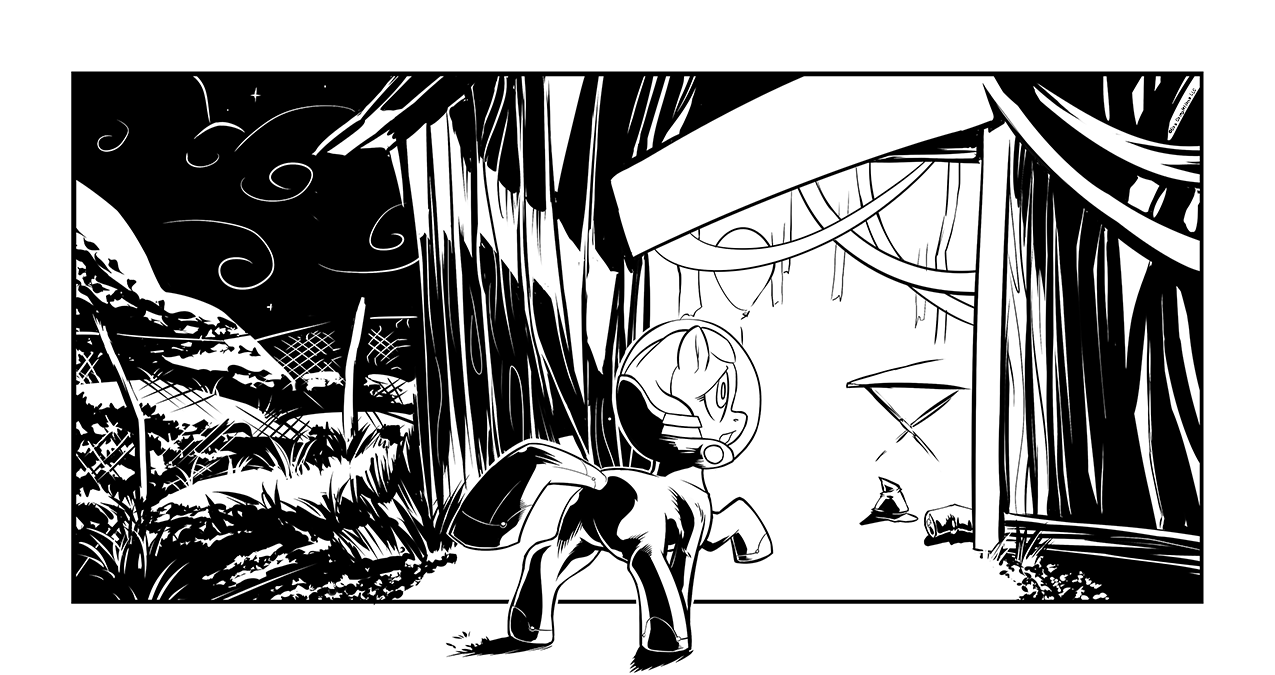
\includegraphics[width=0.9\linewidth]{image02.png}

\begin{intro}
    不需要带上礼物,能来就足够了!
\end{intro}

\daytimeplace{2}{4:00 PM}{赤兔山脉,52号国道北口}{Redtrotters ridges, Big 52 N Branch}

通常来说,穿着一套全封闭式环境适应服一点都不符合小马国时尚审美,但是大家也必须承认它还是能带来很多便利。首先如果你能从一次野火炸弹\footnote{野火炸弹(Balefire Spell):\emph{FoE} 设定之中的几个超聚魔法之一,类似于原子弹}袭击中幸存下来的话,你估计能够享受到渴死在环境服之中的待遇。其次它完全防水,并且基本上隔热,所以你也用不着雨伞或者墨镜。对了还有一点,它是柠檬黄色,所以基本上任何时候你都能被一眼看到。除非……大概……如果……你不小心埋在一大堆柠檬之中的话……那时你肯定不想被任何马看见,对吧?不过,很显然的是在废土上有时候隐匿行踪才是美德。

前提是帕比认识「时尚」这个词的话!

\horizonline

「嗨!我是快乐帕比!」穿着黄色的幼驹对着面前的俩小马微笑着。他们穿着和那天晚上那仨差不多。不过外表少了一些狂野,而且装备更精良。一只独角兽雌驹拿着一把防暴霰弹枪,搜寻着帕比后方是否有什么异常,另一只陆马身边似乎捆着一根大号长矛。要是帕比知道那是什么东西,这两匹雌驹的举动肯定会让她胆怯。

独角兽先开了口:「小鬼,你在赤兔的地盘上干什么?」

「那奇怪的衣服又是什么玩意儿?」陆马接着问。

「我在找我妈妈!」帕比兴奋地回答,伸出蹄子指着路的大概方向。「她在那边!」

俩部族小马相互对视了一眼,然后独角兽又问:「好吧,你妈妈叫什么名字,她是赤兔的?」

「啥是赤兔?」

独角兽的表情开始不耐烦了,不过陆马替她回答了问题。「我们就是赤兔。在52国道上从这里到盐块城都是我们的地盘,所以你想要通过这里,那么你就要通过我们的地盘,所以你妈叫什么?」

「我妈妈叫阴雨·黛丝(Rainy Days)!她超级酷而且总是给我唱歌,还会做很多好吃的!她是最棒的小马!等长大了我也要变成她那样!」

「好了,好了,我知道了。」独角兽不爽地打断她。「抱歉小鬼,但是我不认得什么阴雨,她肯定不是赤兔,你是独自一马吗?谁送你到这儿来的?」

「我有声音先生陪着我!」

「声音先生?」独角兽再次警惕地巡视着道路。

「是啊!他住在我的太空服里,有时候我们一起唱歌,但有时他的脾气也很暴躁,但没关系,因为他会帮我找到妈妈!」

「好吧。」雌驹松懈了警惕。「这样,我很抱歉,但如果你和你的隐形朋友想要通过这里,就得交路费。」

「啊……好滴?我有……」帕比开始在她衣服上的口袋上翻找起来,一路上她收集了不少好东西,大多是一些坏掉的玩具,还有她觉得有趣的东西。或许她可以分一些给这些小马。毕竟我们要彼此体谅,彼此分享\footnote{彼此分享,彼此体谅(You gotta care, you gotta share):这是S01E21中萍琪派的歌词},不是么?

「那么这个怎么样?」

不能用牙齿拿东西是一个很大的问题。她不得不改用她的蹄子,但笨重的橡胶靴使这项任务变得更加艰巨,而且她必须以十分尴尬的角度弯曲她的腿以便伸入她的鞍包。

「等等,我马上就能……呃……」

「{\mt 提示:该防护衣提供简单的操作魔法,可以通过HUD菜单来访问您的物品栏选择物品。}」

「啥?」

陆马看着帕比嘟哝着从她的鞍包中捣鼓出各种无用的垃圾。这个小家伙肯定没有什么值钱的东西。拿长矛的小马看着她的朋友使了个眼色。她若有所思地叹了口气,在对残酷的命运之神进行了短暂地内心祈祷之后,将长矛插入了小马驹的脖子上。快乐帕比忙着听她那衣服发出的各种抱怨。她像一堆砖头一样倒在地上,陆马将她放倒后,默默地咒骂着废土。

「你这是帮了她。如果没有她母亲,她连一天都活不下去,而且我们也不能把她带进来。这样总比让她被蝎尾狮吃掉好,或者比那更惨。你知道这里的小马驹会发生什么。」独角兽叹了个口气。

陆马注意到了独角兽的复杂表情,她补充道:「是啊,可怜的瑞吉……」

长毛马从尸体上拔出武器。当她退后一步时,粉红色的烟雾开始从衣服上的洞中逸出。雌驹注视着这个现象,疑惑不解。「嘿,瘦子,那是什么?」

独角兽用蹄子抓了抓头,「你肯定戳坏了防护服的某个魔法晶片……这东西可能有毒,我们站远点。」

「我们总不能把尸体留在这儿吧,感觉不太好。」陆马犹豫着,但还是躲开了粉烟。

「在你弄出那么多烟火之后,我可不打算靠近她!红蟑螂会解决她的。我们走吧,继续巡逻。」

俩小马最后看了倒在地上的小幼驹一眼,小跑着走开了,离开大路,然后爬过一个低矮的山脊,消失了。时间从路中间黄色幼驹的身体中流过。一阵冷风刮来,在光秃秃的树上沙沙作响。尽管有风,围绕着她的粉红色的云烟似乎也没有消散。

\horizonline

\daytimeplace{2}{4:30 PM}{赤兔山脉,52号国道北口}{Redtrotters ridges, Big 52 N Branch}

在一阵咯咯声之中,防护服发出的声音表示这个故事还能继续讲下去。

「{\mt 初始化系统。检查版本。警告,版本号匹配错误。启用安全模式。版本 0.2。检查装备状态。所有系统上线。检查到大型破损。激活修复魔法。恢复上次会话。读取目标001的个性化信息:快乐帕比,目标已死亡,体征稳定,检测完毕。}」

帕比的双眸在头盔里面眨了眨,就好像她刚刚睡醒了一场长觉。小幼驹打着哈欠,一滴粉色的口水从嘴角落在玻璃面罩上,但是立刻就被玻璃吸收了。

「唔唔……再睡五分钟,妈妈……」幼驹打了个滚,依然被那慢慢消散的粉云包围着。

「{\mt 破损修复,目标已经与危险环境隔离。}」

小雌驹睡眼惺忪地看着四周,先是皱着眉头,然后她似乎想起来什么。「哦,对了,妈妈不在,我刚刚怎么睡着了?」帕比想抓抓头但是蹄子被头盔挡住了。所以她眉头皱得更深了,非常不开心地耸了耸肩,并且若有所思地抱着头盔。

「{\mt 读取临时记忆,提示:失去信号之前最后一个行动,商谈买路钱。}」

「商谈啥?」

「{\mt 与赤兔商谈经过领土的通行费用。}」

% NOTE: 漏译

又来了。「鱼翅……啥?」

「{\mt 和漂漂小马聊天。}」

终于,小幼驹听懂了!「哦,对哦,漂漂小马!我想起来了!啊……他们哪去了?」

「{\mt 赤兔位置未知。将寻找该目标增加到任务清单中。}」

帕比一脸为难的抬起眉毛。「你们还要列个清单?从什么时候开始?」

「{\mt 清单在23小时之前创建。清单上项目:4项}」

「哇哦,我们还真有不少事1、2……呃……4是个好大的数啊,是吧?清单上有什么?」

「{\mt 主要目标:到达MoM。次要目标:解决防护服问题。次要目标:确认马尾伯爵或者至少回避他。次要目标:寻找赤兔。}」

在听完这个清单之后,一脸沉思表情的黄色幼驹戳着自己的头盔。「动动脑子,动动脑子……马芬!不……等等……不是那个……」几分钟之后,幼驹点了点头,双眸闪着光,「哦哦哦!放点音乐……啊……那个话挺多的小马台。」帕比一边听着广播,一边跟着箭头继续她的旅程。

52国道附近的荒地全都是小山和石头,这个地形的视野非常糟糕。这通常会带来很多不便,不过帕比一点都不在乎。

「嘿,声音先生,你刚才说什么关于口袋里面拿东西的事情?」

「{\mt 肯定。这个衣服装备了基础的操作魔法。}」

「呃……怎么用?」

「{\mt 读取说明。选择为幼驹和小呆准备的简单版。说出你要的物品名字,符合描述的物品会悬浮到你面前。}」

「啊……马芬!」一盒200多年前的马芬浮到了帕比面前,她咯咯的笑着,这东西在天上飘着的样子看起来傻乎乎的。

「嘿嘿,好好玩!黎明沙士!」一瓶黎明沙士代替了马芬。「玩具车!」这次一个看起来坏得很厉害的玩具车浮在了幼驹面前。「嘿嘿!我们应该多找点东西,我喜欢这个猜谜游戏!」

「{\mt 否定。这不是猜谜游戏,这是物品管理系统。}」

帕比拿起一块石头放进口袋里面。「石头!」石头立刻浮在了她面前。「耶!真灵!」当石头放回去的时候,石头的名字变成了「命运之石(The Rock Of Destiny)」,但是帕比基本不识字,所以她也没注意。

幼驹一边继续顺着路走着。一边不停地要着物品栏中的东西,其实并没有多少,总共她也只有四件东西,但是她有个大计划。

「哦,我们需要更多音乐!」

\begin{music}
千里之外那指路之星闪耀天穹

\begin{englishlyric}
    I can see that lone star from a thousand miles away
\end{englishlyric}

\medskip

指引迷失的我踏上家乡的归途。

\begin{englishlyric}
    Calling me back home, though I ventured far astray.
\end{englishlyric}

\medskip

当我向着那个灯塔勇往直前,

\begin{englishlyric}
    When I see that beacon shining for me all alone,
\end{englishlyric}

\medskip

它带我飞翔带我回到家乡回到小马国!

\begin{englishlyric}
    It calls me back to `Questria and my home!
\end{englishlyric}
\end{music}

\horizonline

\daytimeplace{2}{7:00 PM}{赤兔山脉,52号国道北口}{Redtrotters ridges, Big 52 N Branch}

这里的居民点看起来比棚户区稍微强那么一点点,至少没有拿臭水沟当护城河什么的。它的城墙看起来更像是一辆撞毁在民宅上的旧汽车,而不是什么防御设施。

帕比完全没有在意这些,一路蹦跶进城里,摇头晃脑地唱着电台里面的歌曲,一直到她面前地面上暴起一团尘土。

「嘿!你,我说了,给老子站住!」

帕比回头看着「城墙」,大概50多米远的地方有个小马举着一个大枪对着她。于是幼驹坐下来挥着蹄子微笑着。「嗨!我是快乐帕比!」

在那堆破烂后面举着大号来复枪的小马显然没有被她的热情感染到,板着脸说:「好吧,拿下那个大金鱼缸,我要看看你的脸!」

「呃……我真的很想这么做,但是我卡在里面了!」帕比想了想说:「实际上,这件事还在我的清单上!」

「好吧,你行……呆在那里把蹄子和武器都放在我能看得见的地方!」

「我不觉得我有什么武器……我有一块石头,算么?我可以丢它!」她蹦跶着说。

卫兵无奈的以蹄覆面,「喂,大号你去搜她身,你,黄色的小个子,给我乖乖站好!」

「好的,好滴,好得!」帕比笑着,不过她的回答显然让那路障后面的小马不满意。

「回答『是』就行了,只要别耍花招,要想大家都没事,就呆着别乱动,让大号做好他的活。」

棕色的大个子雄性独角兽走到帕比身边,看着幼驹在头盔后面的那张笑脸,她双眸之中的光亮现在小得几乎看不到,完全被头盔上各种HUD的光掩盖了。

「我擦,你穿的这身防辐射服保养得可真好……从没见过这样的……」

「当然!它超黄超聪明的,还可以变戏法!你看!嗯……马芬!」刚刚的那个马芬盒子立刻飘到帕比面前。

「哇哦,内置物品管理系统和次级操作魔法,这东西绝对贵得要死,你从哪儿弄到的?」

「中心城的一个漂漂小马给我的!」

「这么说……你来自中心城?」大号听起来不太相信她说的。

幼驹自豪的点了点头。「没错!」

「就是52号国道能看到的那座大山上的城堡么?」

「就是那儿!」帕比笑着回答。

「哦,怪不得你穿着全封闭防辐射服……好吧,我们别闲扯了……给我看你的通行证。」

帕比茫然的看着棕色独角兽,「我的啥?」

「你没通行证?你来的路上没碰到巡逻么?」

「我看到俩小马,一个像我一样的陆马,还有一个是……犄角……单角……哦哦……独角兽!他们超和善超漂漂!」

「没错,没错……好瘦子和冰苏打」大号打断了她后面的话。「他们没和你提什么买路钱之类的?」

「呃……不太记得了。我们聊了一会,然后我有点犯困他们就丢下我走了。」

「随便从她身上拿点什么然后给她个通行证!」

「呃……好吧……」

那小马搜了搜帕比身上,但是除了石头和衣服没啥东西,他甚至想解开那外套,但是不管他怎么弄看起来都没什么用。「好吧,很抱歉小鬼,我也是迫不得已……」他们给了帕比一个中间染了红色的破锡罐。「给你,给幼驹的特别折扣。」

「我会告诉我妈妈你们对我很好,谢谢你们漂漂小马!」

「就这样吧……说起来,一个幼驹穿着防辐射服自己在52号国道溜达?这里可不是什么好地方……」

「我去找妈妈!」帕比看了看附近似乎想要找个标志物,然后指着东南方说:「就是那边,好了我走了拜拜!」幼驹不等他们回答就走掉了。

「但是在哪个方向的就只有嘉年华……啊等一下小鬼!那里很危险,别去那里!」大号举起蹄子,但是转念一想,她和他非亲非故,在废土这种地方多一事不如少一事。

黄色的小雌驹继续顺着小路往前走,她看到那条弯弯曲曲的小路上有一些马为的痕迹,不知道谁在路里埋了很多削尖木棍。帕比在小路上闻了闻,然后就再没管它,在石头上爬上爬下,跳来跳去的游戏对于一个这么大的小幼驹来说是超有趣的。随着夜色慢慢变深,幼驹也渐渐走进废土深处。

\horizonline

\daytimeplace{2}{10:30 PM}{嘉年华,废土}{The Carnival, Wasteland}

一个巨大的谷仓坐落在小小山谷之中,从上面斑驳褪色的痕迹可以看得出它曾经漆成粉色。它被环绕山脊的栅栏包围着,栅栏上每隔一段就有一个自动炮台。这幢建筑和栅栏还有炮台都已经破旧不堪,但是那些炮台依然颤颤巍巍地来回转动着保卫这里。

「{\mt 警告,侦测到自动防御炮台,敌对模式。威胁等级:中等。}」

敌对这个单词让帕比立刻警觉起来,她站定了看了看四周,「那伯爵又来了?在在哪?那马还真纠缠不休,呃,我觉得还是小心驶得万年船。」小小马连忙躲在一个石头后面,警惕地看着那个马尾伯爵先生是不是追来了。「关了音乐,声音先生,我们在躲猫猫呢!」她屏住呼吸竖起耳朵听着周围。

「{\mt 开始和防御系统建立通讯连接。交换协议。申请进入。申请成功。路障已清除,请继续前进。}」

「我说安静!附近肯定有小马……或许是那伯爵,我们应该超级小心!」帕比从掩体后面探出头来,回头看着附近以免有什么可怕的东西就在她身后,然后她慢慢走过栅栏,炮塔马上指向她的方向,但是它们在罗盘上的红点从红色变成了粉色,炮塔又回到了它们通常的防御方向。

「嘿,声音先生……我叫你别放音乐了……」

「{\mt 肯定。无线电已静默。}」

「那么为啥我还能听见音乐?」

「{\mt 声源检测。音乐来自MoM建筑物。}」

「里面?妈妈在谷仓里面?还有音乐和其它东西?妈妈在开派对?耶!」帕比立刻停止了躲藏,四蹄并用从山坡上直奔谷仓大门,最后幼驹猛地踢开大门跳了进去。

「惊喜!」

谷仓里面的空间非常大,而且很开阔,还有两个阁台,一个在门上方,另一个在对面。地面整理得很平,并且铺了一层稻草,墙壁上挂满了破旧的彩带和花环。屋顶上吊着几个看起来很惨的糖罐,还有一大堆灯泡、没气的气球还有其它破烂不堪的旧东西。几盏勉强能发出光亮的旧挂灯无精打采地照亮着这里,唯一看起来能正常工作的就是那个凑合能发出点儿声音的破旧喇叭。

在屋子的正中间有一个派对长桌,桌边已经有一些客人了——一袋面粉,一堆石头,一个装了不知道已经烂掉的什么东西的锈桶,它们都带着一个派对帽\footnote{此处可参考正剧《独马派对》}。哦,座位上还有很多骷髅,至少一打了无生机的小马坐在桌子边,头上带着派对帽,空旷的眼洞看着面前空空如也的盘子,甚至有几个看起来像是干掉的木乃伊而不是骷髅。实际上,其中之一看起来像个饿到皮包骨的小马,而远处的角落堆着一大堆白骨。

「{\mt 警告,侦测到轻微辐射。警告,空气中检测到毒气。分析中,毒气成分:一氧化二氮\footnote{一氧化二氮:无色有甜味气体,又称笑气}。威胁等级:微不足道。}」

「哦,看呐,新客人!」一个看起来像是派对主持的影子从座位上站了起来。那是一只金属的小马,发出旧唱片一样的吱吱声。在昏暗的灯光下,她看起来就像是一只长着粉色鬃毛的粉色小马,但是靠近之后,帕比发现到她是靠轮子移动的,就好像她蹄子下面穿了电动滑冰鞋一样!「看看你的样子!我想你是来这里参加化妆舞会的,不过我很抱歉通知你舞会已经取消了!但是你可以继续穿着你的外套!因为超酷!」另外一件奇怪的事情是,一般小马说话的时候嘴巴会动,但是这个小马印在脸上的微笑却完全不会动,取而代之的是她在说话的时候眼睛却会诡异地闪闪发光。

「呃……你是个……机器马?」帕比迟疑着问,因为她想起来妈妈告诉她如果其他小马看起来很奇怪不要随便当众说出来。

「那是,当然!你真是个聪明的小马!我是娱乐用机器萍琪 MK II 原型 03 号,这是我的生日派对!想要加入么!我可以给你腾出位置,你知道的,有些客人有些不开心,坐在那里不说话。」

「呃……我是快乐帕比……我……呃……我找我妈妈……她应该在这边……大概?」

「太棒了!等她来之后她可以一起加入我们!现在坐下来,你想要吃点蛋糕么?」

帕比没有参加派对的兴致,她应该能在这里找到自己的妈妈,而不是这个破烂生日派对……或许和这个机器马一起玩一会之后她可以帮她。所以幼驹坐在位置上之后看着其他客人。

诡异这个词已经不能形容现在帕比的情况了。那些骷髅正在看着她,所有那些死掉的东西还打扮得像派对来宾一样,尤其是那俩超级瘦的木乃伊……

等等!一个木乃伊居然转过头来了?「求你……哈哈哈……别让我……哈哈哈……笑了……」她还说话了!

这个小木乃伊是一只有着浅黄色毛皮和橘色鬃毛的独角兽,她看起来病得很厉害,幼驹笑个不停但是看起来却一点都不开心,似乎她只是止不住要笑。她眼睛很空洞,而且鼻血流个不停,鲜红的鼻血流得她浑身都是。「求……呵呵……让我回家……」她喃喃地说着这些话,似乎她已经说了上千次,可她仍然在不停地说着,好像说够了次数之后就能从这个噩梦醒来一样。

帕比感觉背后一阵恶寒,好像后背滑过一块冰块似的。这地方不对劲,她想走。但是妈妈在这里,她可能……可能是……那堆……骷髅的……其中之一。

惊恐万状的帕比几乎不能自已。这简直就是那个原本超级和善的机器马觉得烦了,于是就开始伤害小马的故事翻版!已经有太多的小马死在这个毛骨悚然的嘉年华派对上,而马上还会有更多牺牲品!而且她妈妈可能还在邀请名单上,如果她……不对如果她已经……等等!那机器马似乎说了什么她不在这里的话?但是那个机器马可能在说谎。她会说谎么?谁还管这个!这个粉色的东西绝对是个大坏蛋,帕比不想再和她玩了!

那一瞬间,帕比的视线和那个坐在桌边咯咯笑的小幼驹相交,那小马也想她自己的母亲,这里是个坏地方!「快跑,快回家!」帕比看着她,一直到小独角兽离开座位。机器萍琪走过去打算拦住她,但是帕比正要找它算账。

「我妈妈在哪里?」她从座位站起来问。

「等派对结束我们可以一起去找你妈妈,好吗?要不要来点儿黎明沙士呀?」

小独角兽趁机一步一捱地挪向门口。

「抱歉,派对还没结束,你不能走!」

「我妈妈在哪里?」帕比走向那个粉色的马形机械,吸引她的注意。

「好了,好了,乖乖的,别坏了派对兴致。你想玩钉马尾游戏么?」

粉色的火花在帕比双眸中燃烧。「我妈妈在哪里?你把她怎么了?」

「错误。物件妈妈未找到。拜托,别生气。我觉得你妈妈很快就会来接你的!」小独角兽回头看了一眼,靠着大门勉强让自己站好,她颤颤巍巍地走着就像一个乌龟一样。机器萍琪滚着轮子走向她。「站住别动!长辈没允许,不准离开!」

「不要忽视我!她应该在这里的!讨厌的机器马!我不会让你再伤害别的小马,不会让你伤害我妈妈!」帕比低头弓起身子,「石头!」她低声咆哮着。

「请不要说脏字,开始镇压行动,目标免疫毒气,需要使用物理力量,建议使……」

咣当!

「我!」帕比双眸明亮地闪烁着,头盔上反射着粉色的火光,黄色的幼驹直接跳在机器马脸上,不停地用「命运之石」用力砸她。

「妈妈!」帕比咆哮着用双蹄抓着机器马的脖子,拿出自己吃奶的力气和它头碰头,力气大到头盔上都撞出了蜘蛛网一般的裂痕,同时也撞坏了机器萍琪的脸部面板,露出了后面的电路和机械组件。

「在!」帕比一只蹄子继续抓着机器马的脖子,另一只蹄子不停地砸着漏出来的电线,每一下都会让机器马脸上飞出一些被打烂的电路和零件,直到她砸到一个魔法晶片。紧接着机器马就像身体里塞满了粉色和黄色烟花一般炸开了,把帕比炸飞到房间另一头。

「哪里?」被炸飞的帕比一屁股坐在了一座自动炮台上,这东西在她打烂了那机器萍琪之后就冒了出来,电子的爆裂声就像是在悲鸣,那炮台顿时爆成了一团火花,剩下的炮塔则锁定了帕比射出无数五颜六色的激光弹幕,不过那些光线完全无法射穿帕比的防护服。

「别闹了!告诉我,我妈妈去哪了?」帕比径直冲向其中一个炮台,用力撞向它,撞得它歪向一边,而那炮塔还在疯狂的射击着,所有弹幕都打在了天花板上,对于破旧的木质建筑而言,激光的破坏力可比对一件涂有反射材料的防护服有效得多,帕比转身一蹄子把它从底座上踢飞了下来。虽然那机器闭嘴了,但是天花板同时也裂开了。

「妈妈!妈妈你去哪了?妈……妈!」完全不管正倒塌在她周围的谷仓,幼驹疯狂地跑向角落的骨头堆。「声音先生,你看见我妈妈了么?她在哪里?」

「{\mt 错误,地点已到达,斗志部分部已经找到。}」

「你又说什么乱七八糟的?我要妈妈!你说她在这里!」

随着最后一声低沉的隆隆声,历史久远的谷仓终于整个垮下来砸在了帕比的小脑袋上。

黎明的第一道光芒照亮了废土之上永远不散去的云层,一个娇小憔悴的独角兽小雌驹从前MoM建筑倒塌的烟尘之中爬出来。炮台静静地躺在哪里,因为已经失去了动力源,就连音乐声也消失了,持续了200年之久的挽歌终于结束。只有几丝火星在废墟之下闷烧着,吞噬着那些残存的朽木。

\horizonline

\daytimeplace{3}{9:15 AM}{嘉年华,废土}{The Carnival, Wasteland}

即使到现在,这个被诅咒的地方依然没有找回安宁。

「我没有让你找这个可怕派对地点,我让你找我妈妈!」废墟下面闷声说。

「{\mt 否定,你说了……}」外套播放了帕比之前说话的录音。「声音先生……妈妈在哪儿?」

「我就是这么说的!」

「{\mt 肯定。斗志部最近的可用分部已经定位并且标示在地图纸上,并且在几小时前已经被设定为主要任务目标。现在它已被摧毁。}」

「不用你说,它爆炸了两次。」

「{\mt 否定。它不可能爆炸两次。主要损害已修复,系统运转正常等待下一步指令。}」

帕比静了静,整理了一下思路。对声音先生凶也没有用,主要是因为没什么东西可以揍,所以她应该聪明点,她是个聪明孩子,对吧!反正那个机器萍琪是这么说的!

「好的好滴好得……覆水难收……或者说,坏谷仓没法修……既然你说妈妈不在这里,那么然后去哪里?」

「{\mt 警告,尽管已经解释完毕,但现在依然有一个重大误……}」

「喂,闭嘴啦!下一个妈妈可能会在的地方是哪里?」声音先生该不会是因为一直干活不能玩,所以闹脾气了吧……笨衣服……

声音沉默了一会,如果他有更复杂的智能的话,他可能会说些别的,或者至少觉得沮丧,但是这个程序就只是为了服从命令,他只能做到这一点。

「{\mt 下一个MoM地点定为主要目标,位置已经显示在罗盘上。}」

在帕比终于把自己从废墟里面挖出来的时候,一个新的粉色箭头出现在罗盘之上。幼驹跳下碎石堆,抖了抖身上的尘土然后说。

「看到了吧,如果你合作的话什么事都这么简单。」

「{\mt 肯定,合作是魔法。}」

一个金属的笑声打断了这场对话让帕比抬起了头,她看到几天前见过的那个嗡嗡响的机器精灵。

「哦,是你啊提问者,嗨!」幼驹微笑着。

「是守望者……不管怎么说这都太无厘头了吧?」

「什么?你说这个派对?你信我的,你啥也没错过,这是最烂的派对,没有之一,所有小马都无聊到死,呃,真的死掉了。」

「那么,找到你妈妈了么?」

「完全没有。」帕比微微皱了皱眉头,然后又笑了起来。「但是我们还有很多地方要看看,所以没问题!她肯定在哪里,对吧?」

「呃……大概……吧?」机器顿了好长一会儿,「顺便,我可以问问你打算去哪么?」

「那边!」小雌驹用蹄子指着,然后补充道,「这次我觉得会走运!」

「所以,你打算检查下一个『MoM』地点?」

「当然!」

机器又一次顿了很久,「你还觉得下次会走运?」

「没错!」

「好吧,的确是,反正已经……很好,帕比,我该走了,祝你旅途愉快。」

「当然,提问者先生!祝你一路顺风!」机器精灵转头飘走了,还大声广播着贪食精灵进行曲。

「哦,对了!声音先生,来点音乐吧!」

\begin{music}
我不想把整个小马国点燃,

\begin{englishlyric}
    I don't want to set Equestria on fire,
\end{englishlyric}

\medskip

我只想点燃你心中的激情!

\begin{englishlyric}
    I just want to start a flame in your heart!
\end{englishlyric}
\end{music}

\horizonline

\daytimeplace{3}{2:00 PM}{赤兔平原,52号国道北口}{Redtrotters Flats, Big 52 N Branch}

帕比回到了52国道。把那些山丘抛在脑后之后,眼前出现的是一望无际的大平原。远处大城市摩天大楼的剪影面前,点缀着近处一些旧农舍的残骸。在路边有很多旧的马车,有一些是轻巧的小车,有一些是载货的大车。它们都面临着同样的命运——独自在路上锈烂。

「嘿!说你呢,等等!」帕比转向叫她的声音来的方向。

黄色的小雌驹看到过来的是昨天那俩母马,她微笑着挥舞着蹄子,她们其中之一在30米开外停了下来,并举起一把突击步枪,另一个慢慢靠近,并且谨慎地举着动力长矛。

「好的,我的神奇小丫头,乖乖站好大家都不会受伤。」

「呃……我们在玩游戏么?」

独角兽继续用枪瞄准着帕比,另一个小马回答道。

「没错,差不多,想要玩么?」

「好棒!我可以先来么?可以么?可以么?可以么?」帕比已经开始和她这个年纪孩子一样兴奋的上蹿下跳了。

「当然,我们玩我问你答游戏,你如果答不上来你就输了!懂么?」

「耶!猜谜游戏!我超喜欢猜谜游戏!问我,问我什么都行!」

「好,第一问:为什么你嗓子眼被动力长矛戳过之后还活着?」

「啥和啥?」这个问题太难了,帕比完全不知道什么是动力长矛,听起来似乎是吞下什么东西并且不被噎到的意思。「呃……可以略过这个问题么?」

俩母马交换了一个眼神。「或许,这家伙只是个笨小孩?」陆马提议道,独角兽叹了口气,「好吧,我们问问别的事情。」

「好吧,小鬼,那么……为什么你去嘉年华?」

「你是说那个旧农场?好吧,这个傻蛋声音先生告诉我妈妈在那里,你猜结果怎么回事?她没在那里,而且那里还有个全世界最无聊的派对,那个发疯的粉色机器马还想伤害我妈妈,我很生气,但是机器马爆炸了,然后有个怪东西开始往我身上照讨厌的光线,剩下的我记不太清了,只记得整个农舍都砸我头上了,最近真是被房子砸了好几次……」帕比想了一会,又补充道。「我希望那个瘦瘦的孩子能安全回家。」

「瑞吉还活着,所以我朋友还没开枪打你。」陆马深吸了一口气。「所以你复活了以后走了这么远跑到嘉年华,然后把那个天杀的地方毁了,并且救了瘦子的妹妹,这一切只是个意外?」

「我……我不记得我做了那些事情,不过既然你这么说……」

「然后你一直只是在找你妈妈?」雌驹抬起眉毛,疑惑地问道。

「是的,你知道她在哪?」

「没错,她就只是个笨小孩。」陆马无奈地以蹄覆面,而独角兽在她身后大笑着。

笑过之后,独角兽表情变得严肃起来。「不管怎么说她救了我血亲,我欠她的。」

「那么你想怎么办,瘦子。」陆马问。

「我不知道。」瘦子放下枪口靠近那个冲她微笑的快乐帕比。那天真无邪的小小微笑融化了这个铁血女独角兽的铁石心肠,她将一只蹄子放在帕比头盔上。

「我不知道你是好是坏,不过我欠你一次……所以,谢谢。」瘦子递给她一个金属片,上面刻着一颗吃了一半的白色苹果,「拿着这个,这是通行证,如果你去盐块城,把这个给卫兵看他就会让你进去,懂吗?」

帕比睁大眼睛看着她收到的馈赠。「哇哦,谢谢!礼物,我超喜欢礼物!漂亮的大姐姐非常感谢你!」

独角兽继续说:「你终结了我们一族的噩梦,还救回了我唯一挚爱的血亲,我希望你能找到你所寻找之物,小小幽灵。」

「哦哦哦,你也有这么可爱的时候?」陆马低声揶揄着。

「给我闭嘴,赶紧走,苏打,我们还在巡逻呢!」

「嘿,你哭了,瘦子?」

「你闭嘴好么,绝对不准和其他马提起这件事!」

「好吧,说起来,现在我对之前杀过她有些愧疚了。」

两只小马向着粉色箭头相反的方向走开了,帕比挥着蹄子目送他们消失在山脊之后。

「我喜欢漂漂小马,她们真漂亮!」帕比笑着,然后出发走向大城市。

「嘿,声音先生,我可以问你一些事情么?」

「{\mt 肯定,请陈述您的请求。}」

「等我们找到我妈妈之后,你会离开么?我是说……我不想让你走。」

「{\mt 否定,在幼角药剂的影响下,该装备已经永久与您融合。}」

「呃……这就是说,我们能永远在一起?我找到妈妈以后还能和你在一起?」

「{\mt 肯定。}」

帕比微笑着,和往常一样只听她想要听的事情。

「好的声音先生,你已经知道我们现在该干啥了吧。」

「{\mt 肯定,基于数据分析,对您的日常需求预测现在有95\%的准确率。}」

广播开始播放声音,帕比一边唱一边走下去。

\begin{music}
你和我,在一起,

\begin{englishlyric}
    You and me together will be,
\end{englishlyric}

\medskip

在一起,在一起,

\begin{englishlyric}
    Forever you'll see,
\end{englishlyric}

\medskip

我们是,好姊妹,

% NOTE: 兄弟 -> 姊妹

\begin{englishlyric}
    We two can be good company,
\end{englishlyric}

\medskip

好姊妹,好姊妹

\begin{englishlyric}
    You and me
\end{englishlyric}

\medskip

你和我,好姊妹……

\begin{englishlyric}
    Yes together we two\dots
\end{englishlyric}
\end{music}

\clearpage

~\vfill

\begin{note}
升级。我想我们早讨论过这个问题了吧。

否定。升级是辐射小马国同人的既定内容。

好吧好吧,真烦,我可以理解帕比的心情了,那么这样。

增加任务专长:升级是命令——现在你可以正常升级了,耶!
\end{note}






\chapter{迷路羊群}

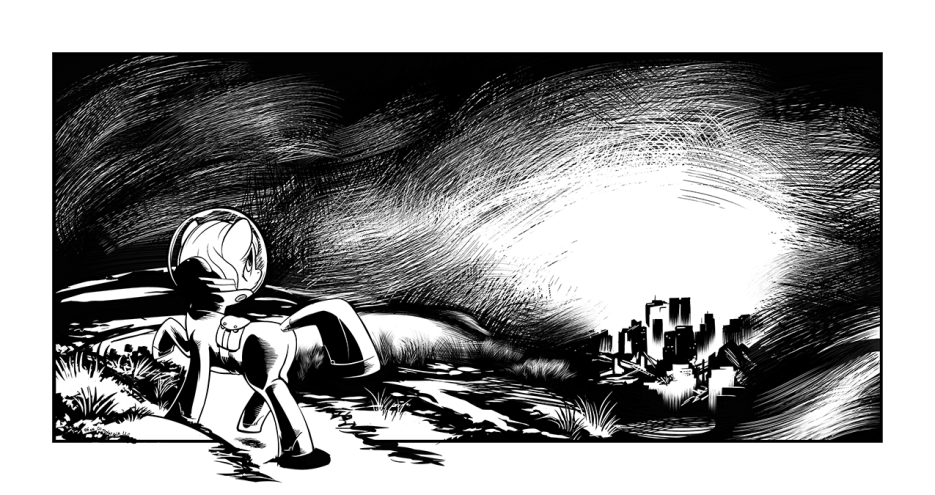
\includegraphics[width=0.9\linewidth]{image03.png}

\begin{intro}
很久很久以前,在逐渐消亡的小马国土地上
\end{intro}

「{\rt 女士们,先生们,晚上好!这里是孤狼\footnote{孤狼(Lonesome Pony):后面缩写为 L.P.}的52电台!虽然,野马 DJ PON-3 尥蹶子踹好了吠城(Fillydephia)的广播晶片,所以十马塔(Tenpony Tower)的广播在整个废土都收得到!但是只有在这里才有你想要听到的所有52国道新闻!}」

然后一阵悠扬的音乐持续了几秒钟。

「{\rt 以上就是大狗\footnote{大狗:这里指孤狼}能提供的全部服务了,现在回到本地新闻。嘿,小马们,你们害怕幽灵吗?也许你们应该害怕。你们记得嘉年华的故事吗?如果没听过不要紧,老朋友L.P.现在就给那些没预习功课的小马们补补课!}」

「{\rt 在52号国道最最最最最北边的地方,有一处大家不知道的农舍,赤兔们叫它嘉年华。那是一个年代久远的遗迹,但是不像它的兄弟姐妹一样,嘉年华从未真正安眠。自从我祖母记事以来,每隔一年就会有一个幽灵从那里出现,游荡在附近的山丘,邀请大家参加她的聚会。当第二天早上来临的时候,就会有小幼驹神秘地消失,然后再也回不来了。感谢那些无处不在的激光炮台,靠近嘉年华几乎是自杀。不过如果你靠得够近,就能听到在那被诅咒的谷仓里面传出音乐声,就像是整天整夜地在狂欢一般。}」

「{\rt 我的小马们,看起来似乎是有谁大喊着『我不怕幽灵!』然后冲进那派对中把整幢农舍的房顶掀翻了。非常勇敢。现在赤兔的小幼驹终于可以安心睡觉了。我很好奇这个神秘的英雄是谁,但是大家都说她也是一个幽灵。是一只在粉云之中穿着黄色防辐射服死而复生的小幼驹。干得好,黄色幽灵。你给废土解决了一个大麻烦,你面前还有一百九十九个要解决!哦,我有提到今年嘉年华的被害者安全回家了吗?塞拉斯蒂娅公主祝福我们!现在还是继续我们的小马萨克斯吧!}」

\begin{music}
我在千里之外看到指路之星,

\begin{englishlyric}
    I can see that lone star from a thousand miles away,
\end{englishlyric}

\medskip

它在远处向我招手叫我回家。

\begin{englishlyric}
    Calling me back home, though I've ventured far away.
\end{englishlyric}

\medskip

指路之星如灯塔般给我带路,

\begin{englishlyric}
    When I see that beacon shining for me all along,
\end{englishlyric}

\medskip

让我回到小马国回到我的家!

\begin{englishlyric}
    It calls me to Equestria and a home!
\end{englishlyric}
\end{music}

\horizonline

\daytimeplace{4}{00:30 AM}{盐块平原,52号国道北口}{Salt Cube Flats, Big 52 N Branch}

帕比顺着52国道一路向南,远处大城市的剪影从地平线上跃升成为一个高楼林立的巨大水泥丛林。幼驹走了整整一天,而现在阳光消逝在黑暗之中。小雌驹眼睛中闪烁着的亮粉色光芒照亮了她的道路,虽然没有阳光,但还是可以清楚地看到盐块城那个微微发光的圆顶建筑,还有几座巍峨的摩天大厦耸立在一片漆黑的废墟之中。

差不多午夜的时候,小雌驹看到一个小车队从他的方向一起往南走,大概有半打小马和非常非常奇怪的……有两个脑袋的牛跟着他们?帕比惊奇地坐在地上,等待着他们靠近。显然车队卫兵也很快发现了幼驹,毕竟她是个坐在路当中的光源。当然,卫兵做好了战斗准备。

一个穿着轻型战斗鞍具的大块头低声问着旁边的小马。「你觉得……这个就是新闻中说的那个『幽灵』吗?」

卫兵的领头,一只带着大号左轮枪的陆马耸了耸肩,举起蹄子示意车队停下来。

「不清楚,但是我不冒险,所以我们慢慢来,你们俩去旁边,另外俩站在这里,我去交涉,好好掩护我,要不然你们别想领薪水。」

两个卫兵离开车队向旁边的小路前进,绕到帕比的侧翼,同时领头走出车队,两个卫兵保持距离守在后面。小雌驹的样子看起来很诡异,一个发出粉色光芒的大圆头盔安在一个小小的黄色轮廓上,不过的确是个很明显的靶子,卫兵领队一边小心靠近,一边祈祷她的卫兵在发生什么突发状况的时候能够救她一命。

「嗨!我是快乐帕比!」幼驹举起一只蹄子向领队挥舞着。好吧,至少她看起来还算友善。

不过在废土生存指南上,不止一次强调过「有备无患——看起来友善不等于安全。」

「好吧,站在那里别动,说个不让我把你变成一堆化肥的理由。」

帕比咯咯笑着,奇怪的话总能逗乐她。「喂喂,漂漂小马爱说笑!我不叫华菲!我是帕比,你叫什么名字?」

卫兵头头迟疑着,这个幼驹只是在冒傻气还是给她设了一个精心布置的圈套?但是经验告诉她有哪里不对劲。「对,我是固体虫。你独自旅行?」不等回答,她的卫兵已经开始检查附近了。

「当然不是,我和声音先生一起!他有时候超级聪明有时候超级笨蛋,取决于……不管怎么说他知道我妈妈在哪里啦!」

「那么……这个声音先生又在哪儿?」

「在这个太空服里!看到这些灯和漂亮点点了么?他能让这些东西出现!」

固体虫仔细看了看衣服的头盔,不去管帕比那俩闪闪发光的大眼睛,的确有一个HUD,和一些高级战斗鞍具用的瞄准设备差不多。一看到这个看起来价值连城的上古装备,她很想知道一个幼驹怎么能找到这种好货?但是那粉光总让她觉得不太自在。简单地说,固体虫干了很久护卫,见过废土上的不少东西。

「这么说,你应该是从中心城来的?」

「对哦!我家的房子就在……呃……正好在山脚下的四叶镇,不过有一天它塌了,所以现在我在找我妈妈。她不在声音先生说的一个旧农场,不过他说这个大城市还有另一个大地方。所以我要去那里看看!」帕比用蹄子指着南边说。

固体虫听的时候点了几次头,举起蹄子示意车队可以安全通过。在车队开始前进的时候她说。

「你可真能聊,不是么?孤狼刚讲到你在嘉年华的大冒险\footnote{大冒险:冒险(exploit)和后面的爆炸(explode)似音}。」

「我的啥?你说那个旧农场,我没炸了那里,农场自己爆炸了,小傻瓜。」帕比咯咯笑着。「那个机器萍琪绝对是个坏蛋!虽然开始很可怕,但我可是很勇敢的哦!」

固体虫挠了挠头,不想让帕比在闲扯下去了。「呃,没错,你很棒,我很想继续聊一会儿,但是我们还有事,如果你想去盐块城,那里的尸鬼集会在圆顶里面,我想他们把那里称作『炫彩』。别在城里闲逛,城里的人不喜欢你们。不管怎么说,祝你好运,小幽灵。」

当车队路过的时候,其他小马都好奇地看着帕比,但是固体虫和一个紫色红棕的独角兽说了两句,于是他们继续前进,黄色的幼驹很吃惊地看着那些双头牛,并且拼命地挥着蹄子,一直到他们消失在夜色中,然后她继续独行向南走。

\horizonline

\daytimeplace{4}{11:30 PM}{闹市区,盐块城}{Downtown, Salt Cube City}

这里的大门只是个用沙袋和破金属片堆成的壁垒。在一个木制平台上,有只穿着金属马铠的小马坐在一挺加特林机枪后面,另外两个门卫正在检查每一个想要进盐块城的小马。最后一个穿着军官制服的独角兽则坐在一个金属小房子里面写着什么。

虽然说现在快到正午了,但是城北门外和废土其它地方一样空无一马。这次帕比早有准备,她把那个有着白苹果的铁片给卫兵看。其中一个小马走过来,另外的几个卫兵则举起了武器。

「我看看。没错,就是这个通行证。那么,你叫什么名字,来做啥?」

「我叫快乐帕比!神秘的漂漂马你叫什么呢?」

卫兵抬起头盔的面罩,一脸不爽地看着帕比。「远见下士,好了,现在可以告诉我你来干啥了吧?」

「哦,这个问题我知道!我在找我妈妈!她大概在这个方向!」帕比伸出蹄子指向那堆残破不堪的建筑给卫兵看。

「好吧,够了,还有个问题,为啥你穿着全套环境防护服?」

「哦,这个么?我困在里面出不来了,不过没关系,因为有个狠好心帮助我的神秘声音也住在里面。」然后幼驹小声对远见咬耳朵。「不过他一点也不擅长找谁,不过别和他说,因为他脾气不好。」

卫兵放下面罩耸了耸肩。「只要你不打算在闹市区引爆超聚魔法,你想怎么穿就怎么穿。欢迎来到盐块城,小鬼头。」

幼驹连忙头也不回地跑过路障,但是远见在她身后喊着。「哦,对了,提醒你一下,别接近那个圆顶,因为那里面有野生尸鬼,而且有很多辐射污染。」

「好的好滴好吧!拜拜卫兵远见先生!」帕比跟着粉色箭头的方向,从那几个摩天大楼里穿了过去。

这里的闹市区和52号国道的其它街区差不多,有卫兵在往来巡逻,防止小马们在街上火拼。还有各个不同的贸易公司在街上竖起来的广告牌。比如『水农』或者『飞驰子弹』甚至还有一些雇佣兵和附近一些部落的交易代表。这个完全开放的市场看起来就是城市的中心,不过这个城市的真正中心是那四栋经过百年战争和风雨洗礼依然屹立不倒的摩天大楼。

盐块城在战争中曾经就被一个超聚魔法击中,不过运载超聚魔法的魔法导弹似乎出了一些问题,弹头击中了城市郊区的盐块圆顶,击穿了那个圆顶建筑的房顶,然后在里面爆炸了,坚固的圆顶保护城市免受冲击波的伤害,但是城市还是受到了放射性尘埃的影响。在之后的岁月中,城市里的大多数高楼大厦都在岁月的侵蚀下一个接一个地倒塌。但是那四座基本没有受损的摩天大楼依然在城市中心屹立不倒。

这四座高塔就是盐块城权力的象征:其中两座双子楼曾经是某个大型国际贸易公司的总部,而另一个和他们差不多高的大楼是一个强大的雇佣兵公司——聘蹄(Hired Hooves)的总部,最后一个,也是最小的一个,上面贴着白色苹果标志的大厦。住在里面的是这个城镇的所有者。整个城镇的所有交易都要向他们交税。白苹果同时也是聘蹄的主要兵员提供者,因为聘蹄的很多士兵都是这个家族的小马。

帕比站在一个染着红色印记的帐篷面前——这个印记表示帐篷的所有者是赤兔部落。这个商店的架子里面摆满了各式各样的铠甲和肉搏兵器,一个带着旧牛仔帽的雌驹坐在帐篷中间的一个弹药箱上。

「嘿,穿得不错的小家伙,你是不是从北边来的?」雌驹很富有魅力地笑了笑,用一只蹄子推起牛仔帽。牛仔帽下面露出了她前额上的独角。而在她臀部上的可爱标记看起来像一个棒球棒。

「嗨!我叫快乐帕比!」幼驹挥着蹄子走向雌驹。她指着帐篷外面的方向说:「我从那边来!」

「我叫强攻,我想你就是孤狼昨晚提到的那个家伙。」

「呃,你说那个在音乐频道唠唠叨叨的家伙?」帕比若有所思地挠着她的头盔,「上次我就听他说什么喝纯净水很重要。」

「不,不,我是说你是新闻里面说的那个『黄色幽灵』吧?或许附近不只有一个小马穿着防辐射服闲逛?不管怎么说,你想买点啥?」

帕比皱着眉头,「为啥大家都叫我幽灵?」

强攻笑出声来:「就是你嘛,我就知道!」独角兽轻抚着自己的下巴想了一会,「不管怎么说,作为一个拆了那诅咒农场的英雄,你是不是有点年轻?实际上你这个年龄就你自己在废土上冒险可不应该……你难道是个童子军\footnote{童子军(Crusader):可爱标记童子军的大名在废土上可谓如雷贯耳}?」

「当然不是,我是在找我妈妈!而且我不孤单呢,声音先生陪着我!」

「你妈妈?或许我可以帮你,毕竟我在闹市区认识很多小马,你妈妈叫什么名字?她可爱标记是什么?」

快乐帕比大概描述了一下。「哦,她名字叫阴雨·黛丝,她毛皮是紫色鬃毛是橙色,她的可爱标记是有着雨点的云彩!你见过她么?声音先生说她在这附近!在那边!」帕比指着那个半毁的圆顶说。

强攻摇了摇头。「抱歉,小鬼,完全不记得有这么一个可爱标记的小马,也不记得听过这个名字。」卖货的独角兽皱着眉头看着幼驹指着的方向,「你说那边?那可不是什么好地方,那里辐射很强,而且那里唯一一个比较完好的建筑物就是圆顶,听我的,你绝对不会想到圆顶附近的。」

「圆顶?那是啥?」

「那里到处都是野生尸鬼和其它可怕的东西,虽然说你穿着防辐射服不怕那里的辐射,不过最主要的问题还是那里的居民——一小撮鬼迷心窍的尸鬼。他们基本上就是个会行走的定时炸弹。虽然他们看起来暂时很文明,不过不知道什么时候他们就会发疯攻击小马。而且现在白苹果也正在想办法除掉这些快腐烂的脑袋——他们会打爆每个走出废墟的尸鬼头。但是他们没办法进去检查,如果你不免疫辐射的话,那里面就是个巨大的死亡陷阱,所以他们也束蹄无策。」

帕比皱着眉头问:「尸鬼是什么啊?」

「你……在开玩笑吗?你都不知道尸鬼是什么?」强攻看着帕比脸上的表情,然后说:「好吧,看起来你没开玩笑。尸鬼就是小马被辐射长时间影响的结果。当超聚魔法爆炸的时候,有些小马没有死掉,而是变成了某种……怎么说呢?活跳尸?或许可以说是僵尸?不管怎么说,他们其中一部分变成了野生尸鬼——这些家伙见谁吃谁。还有一些能够保持自己心智的家伙变得永生不死,但是他们身上的肉还是会腐烂,鬃毛也基本掉光。每个尸鬼看起来都像一具正在腐烂的尸体,但是却还活蹦乱跳的。而且最大的问题就是,那些神智清醒的家伙迟早也有一天,脑子里面的神经『嘎嘣』一下,然后就变成了野生尸鬼。」

帕比眉头紧皱,独角兽感觉到她似乎很害怕。

「强攻小姐……呃……如果我妈妈真的在声音先生说的那个地方,她会安全么?」

「我想……」独角兽低下了头,把眼睛藏在帽子下面不去看幼驹那双纯洁的双眸。「我不知道,小幽灵,圆顶是个危险的地方,我只是希望你听我说完之后打消去那里的念头。」

帕比昂首挺胸四蹄站直,眼中的信念无比坚定。「我必须去那里!妈妈也许就在那里,她可能有危险!」

强攻看起来没办法说服她不要去做这个自杀任务。「你和我非亲非故,我没办法叫你不要去那里,但是还是请听听我的意见。到那座高塔那里去,就是有白苹果标记的那座高塔,然后和那里的小马说你想去圆顶里面执行侦察任务,他们或许会给你一些装备和援助,让你安全一点。」

帕比微笑着回答:「好的!我知道了!等着我妈妈,我这就去救你!」幼驹飞奔出帐篷冲向白苹果塔。

\horizonline

\daytimeplace{4}{2:00 PM}{盐块圆顶,盐块城}{Salt Cube Dome, Salt Cube City}

「{\mt 警告,侦测到少量辐射,威胁等级:可忽略。}」

圆顶曾经是一个巨大的椭圆形建筑物,曾经作为一个可以同时举行数个展览会的巨型会馆。一个巨大的球形屋顶把整个建筑物包裹起来,但是现在它基本被摧毁了,剩下一些残垣断壁像是一个超大号的露天体育馆。

在圆顶的正面有一条小道,小道上有一堆石头拱门的残骸。这些残骸看起来曾经是抛光的大理石柱,但是现在只剩下一堆碎石。帕比站在小道的面前,看着罗盘上的粉色箭头。

「好吧声音先生,我们现在要做什么来着?」

「{\mt 士气部分部已经到达,主要任务目标完成。}」

「我知道我们到这里了,我说接下来我们该做什么?」

「{\mt 次要任务目标:和尸鬼交涉并且/或者解决他们。警告,侦测到少量辐射,威胁等级:可忽略。}」

「那么,我们找到那些尸鬼,然后问他们妈妈在哪里,然后赶他们走开?」

「{\mt 肯定。这个说法很接近了。}」

「赞!我喜欢有计划的感觉,我们开工吧!」帕比走进大厅然后大喊,「嘿!尸鬼小马!」她声音的回音在巨大建筑里面回响,但是看起来却没有回答,于是穿黄衣的幼驹慢慢走到大厅的台阶下面。

「{\mt 警告,侦测到大量辐射,威胁等级:可忽略。}」

「嘿,我觉得我看到有谁在那些雕像后面走!喂,你等等!」帕比冲向那个黑影躲藏的大理石柱子后面,她看到一个黑影于是大叫道:「嗨,我是快乐帕比,你有看到我妈……」

是他!是那个家伙!马尾伯爵!他就站在她面前,虽然比她记忆中的还要更丑更可怕。

「{\mt 警告,侦测到敌对生物,野生尸鬼,距离 \SI{2}{m},威胁等级:低。}」

那个生物回头看着帕比的脸,黄色的口水从他嘴里面流出来,他看起来很疑惑,不知道下一步该干啥。

帕比满脸惊恐地看着那个生物后退一步。

「为……为什么你还跟着我?走开!走开!!」

那生物面对帕比嘶吼着低下头,而后者则撒开四蹄以她最快的速度逃命。

不过她跑得还是不够快。

头盔的设计就是为了抵御外来伤害,所以这个野兽的攻击只是让帕比幼小的心灵受到了惊吓。一口腐烂的,锯齿状的牙齿刮擦着她头盔上的画面,以及那尖锐的摩擦声就足够把她吓傻。

「咿咿咿咿咿咿呀呀呀呀呀呀……!」帕比本能地用力踢着那个尸鬼,但是那东西比一个幼驹实在重太多。

「石头,给我石头!快!」

幼驹一边尖叫着一边用双蹄抓起漂浮到她面前的「命运之石」,然后用力地砸向那个怪物。

「给我停下,停下!快停下!」

几分钟之后,帕比还在用石头用力砸着一滩棕色肉泥,这东西曾经是一个小马的脑袋。头盔上的划痕和一些划破的衣服在自动修复法术的作用下已经消失。最后尸鬼已经完全不会动,而帕比也需要喘口气。

虽然刚刚好可怕,但是马尾伯爵已经被消灭了!她最糟糕的梦魇已经消失,再也不用逃跑或者躲躲藏藏了!帕比大大松了一口气,然后把自己的视线从死掉的尸鬼身上挪开。

不过她马上就注意到另外三个尸鬼正在用同样空洞的眼神流着口水看着她。

「{\mt 警告,侦测到敌对生物,数量 3,最近目标:\SI{12}{m}。}」

「喂,声音先生。你说的无解还是误劫的那东西是啥意思?」

「{\mt 误解,错误的理解一个词语和句子的意思。}」

帕比一边看着三个尸鬼一边慢慢点点头。

「那好,你说的马尾伯爵到底是什么意思?」

「{\mt 敌对生物数量。在感应器范围内有攻击性的生物。现在敌对生物数量3,种类:野生尸鬼,威胁等级:中等。}」

帕比叹了一口气,举起石头冲向尸鬼,而尸鬼也同样冲了过来。

\horizonline

\daytimeplace{4}{2:30 PM}{盐块圆顶,盐块城}{Salt Cube Dome, Salt Cube City}

「{\mt 警告,外衣密封性遭到破坏。警告,侦测到幼角药剂。警告,罗盘无法工作。警告,物品管理系统离线。警告,能量水晶遭到破坏。能量火花剩余29.06\%。警告,侦测到致死剂量辐射,威胁等级:可忽略。主体已死亡,生体指数稳定。检测完毕。}」

帕比完全站在一个大屠杀场景的中央,身上沾满了粘液和碎肉,三个尸鬼的无头尸体横七竖八地躺在她身边。这场战斗打了这么久的原因是因为帕比站在了强辐射区中间,只是尸鬼的重生能力最后还是输给了粉色药剂和帕比防辐射服的自动修复魔法。而且比起那些只知道乱咬的尸鬼,帕比能够用石头不停地打他们的脑袋。不过她也和一个沙袋一样被踢咬了很多下。她的臀部大半都被吃掉了,剩下大团粉雾包裹着那里。

「我说,声音先生……你确定妈妈在这里?」

「{\mt 肯定,准确位置:斗志部建筑编号:00201——盐块城圆顶。}」

「好吧……好滴……好得……」帕比已经听够了『肯定』,在战斗中精疲力竭的她现在很不爽地踢着地上的土。「为啥我现在只想哭呢?」

几个小马身影出现在大厅的另一端,他们看起来似乎在低声耳语着,其中之一拿着一杆猎枪,而另一个小心地接近黄色幼驹,帕比伸出蹄子抓住落在一边的「命运之石」,但是她现在很累,只想再多躺一会。「拜托……别欺负人家……走开……我是乖孩子……」

帕比看清了走进的那个小马,它是另一个尸鬼,但是却和其他尸鬼不太一样,这一个穿着和给她外套的雌驹一样的白大褂,就是脏了很多。而且在它的眼中可以看到智慧的光芒,而且最后一点,它说话了。

「嘿,你还好吗小家伙?这里非常危险。」这个小马的声音就像是粉笔在黑板上的刮擦声音,不过帕比依稀觉得它应该是雌驹。

「我说,软气!趁她还没受辐射伤之前赶紧把这个小家伙从辐射区拖出来!我们还有辐特宁之类的么?」

「我觉得没有必要,躲开那些粉云,那东西看起来很熟悉,我可以肯定那是什么危险品。」

跑来侦查的小马听到之后停了下来,歪着头看着那团粉雾。

「我的天,我的眼睛坏了么?」尸鬼说着绕了一圈,那些粉雾很快就消失了,就好像幼驹的外套在自我修复过程中把粉雾吸了回去一样。

「{\mt 外衣密封性恢复。警告,侦测到致死剂量辐射,威胁等级:可忽略。}」

看着尸鬼雌驹慢慢靠近,帕比依然举着她的小小『武器』。幼驹想还是应该先礼后兵。「我……那个……我想这些丑丑马不是你的朋友吧?」

「你是想说『尸鬼』吧,小家伙。好吧,确切的说他们曾经是我的朋友,不过我觉得你现在是帮了他们一个忙。所以,没有好马受伤。」

尸鬼雌驹站在帕比面前看着头盔里面,幼驹虽然看起来有些不开心,但是完全没有任何伤痕或者腐烂的迹象。只是在她的眼眸之中燃烧着明亮的粉色,而且她的说话声音也比普通孩子大那么一点。「你还真是个奇怪的尸鬼,我叫桃花,你叫什么名字?」

「呃,哦哦,对哦,我叫快乐帕比,我正在找我妈妈,她应该在这附近,但是我见到的都是些丑马。」

桃花挥着蹄子招呼她的伙伴:「软气,别发呆赶紧过来!」

然后她回头继续和黄色的幼驹说。「你能不说我们是丑丑马么,叫我们尸鬼,而且如果你妈妈在这里她也应该是个尸鬼,或者是个超级史莱姆什么的。你妈妈叫什么名字?」

「这个问题我知道!她叫阴雨·黛丝而且超级酷!你见过她么?」

走过来的那个家伙听到之后说:「阴雨……阴雨……这个名字听起来好熟,你让我好好想想,我好像记得有这个名字?」

帕比一脸惊奇地看着软气,「真的?拜托拜托拜托!她在哪?」

「喂喂,等一下,我说了我记得不太清楚!我记性已经不如从前那么好了……不管怎么说,如果你不想再碰上其他野生尸鬼,那么我们还是赶快走吧,去炫彩大厅(The Glow)。」

桃花点了点头:「没错,我们赶紧走吧,反正我们找到要找的东西了,呃,帕比,你从哪儿来的?」

「中心城!」帕比自豪地挺起胸。中心城是最棒的城市,为什么不自豪呢?

两个尸鬼都皱起了眉头,桃花扭开了脸,而软气长叹一声。

「哦,原来你是那种东西啊。」桃花喃喃自语着。「烂透了的战争。」

\horizonline

\daytimeplace{4}{3:00 PM}{炫彩大厅,盐块城}{The Glow, Salt Cube City}

炫彩大厅其实只是这个圆顶中心的一个尖顶小屋。这里的圆顶早已不复存在,满地都是各种废墟。小屋上有着三个粉色的蝴蝶标记,小屋的坚固材料在两个世纪的风吹雨打中都没有损坏。

不过这里叫做炫彩大厅的原因不是因为小屋也不是因为尸鬼,这里正中央有一个十二米高的大方块正发出绿色的荧光\footnote{辐射荧光:切伦科夫效应,但不是所有辐射现象都会有明显的切伦科夫效应,所以该解释仅供参考}。

「{\mt 警告,辐射等级超出量程,探测器紧急关闭以避免受到永久损坏。威胁等级:可忽忽忽忽忽……}」

头盔的HUD忽然消失了,帕比皱起了眉头。然后又耸耸肩,就算是声音先生也许有时候也想要去睡一觉吧。

中间的方块此刻吸引了帕比的全部注意力。那个透明的方块发出超级漂亮的光芒,幼驹希望能有个一样的小方块放在自己卧室里面,这东西一定能吓跑她床底下那些坏怪物。然后有那么一瞬间幼驹想起自己的房子,只觉得鼻子一酸。但是想到自己是一个正在执行任务的小马,她没有时间去哭鼻子,所以她问道:「那个漂亮的发光方块是什么?我也能有个发光方块么?拜托,超级拜托?」

软气笑出声来:「我想不行,帕比,不过如果你做个乖孩子我可以给你点儿别的,可以么?」

帕比开心的蹦来蹦去:「礼物?给我的?快给我,给我,给我!」

「好,好……不过做个乖孩子,好么?首先我们要和沙盒聊聊,然后我们去找找看阴雨小姐。」

帕比立刻安静下来,乖乖地跟在软气和桃花身边。「那个……就算你们超级丑,但是你们超级有趣而且超级和善!」

桃花一脸的不爽:「好吧,多谢夸奖,怪物小姐,好了,就是他了,沙盒,这个营地的头头。」

另一个尸鬼正在看着一摞纸,并且不断地挠着头。

「就算有时候他看起来有点秀逗,不过他也比其他科学家要聪明很多。嘿,老大,我们有客人了。」

尸鬼的领导穿着一件老旧的白大褂,戴着一副眼镜。他看起来对那些纸上的内容显得有些不安。他看都没看帕比一眼就回答道:「真好,告诉他我们的规矩,警告他别去闹市区,很抱歉我现在不想聊天。」

帕比咯咯笑着走到他面前,看着他的脸说:「呀,丑丑马也会说奇怪的话!嗨,我叫快乐帕比,你叫我帕比也行!你见到我妈妈了么?」

桃花一回头那幼驹就跑过去了,想要拦都拦不住。尸鬼卫兵正想解释的时候,却被她头领阻止了。沙盒推了推他的眼镜,盯着帕比研究了一会之后,忽然大叫起来。

「哦,我的露娜小蹄子!这难道是又一套能正常工作的 Mark VI 么?这可真是个奇迹,不是么?」

桃花和软气都一脸茫然的看着他们的老大,但是沙盒完全不在意其他小马的表情,只是继续说下去:「这东西本来设计目的是为了保护幼驹不受到辐射尘的影响,里面安装了最先进的医疗魔法护符和最新的逻辑魔法回路——你知道的,避难厩科技(Stable Tech)制造的哔哔小马\footnote{哔哔小马(PipBuck):详细介绍可以参考 \emph{FoE} 序章的内容}用的那种。」尸鬼摇了摇头,他的兴奋之情变成了哀伤,「但是我们没有预料到的是,这些科技和魔法在粉色药剂下产生的结果:这件外套的医疗补给和医疗魔法护符缓和了毒气的致命效果,创造了最佳的……恩……『融合』环境。」

那个科学家转头对其他两个尸鬼说:「你们听说过幽灵羊群么?」两个小马摇摇头,沙盒把蹄子放在帕比肩膀上,让她站在他身边。

「那是女神陨落大概一个月之后的事情,一小群和这个孩子一样穿着黄色防护服的幼驹离开中心城,他们之中大多数都已经因为突变而失去心智,而其他的幼驹完全不知道发生了什么。他们的确是幽灵:因为中心城的大屠杀而失去自己双亲,他们在一起只是因为他们认识的其他小马都已经死了。就这样漫无目标的一路向南前进,虽然路上遇到一些幸存者,但是那些已经发疯的小孩只知道把他们见到的所有活物撕成碎片。其他的孩子……他们只是不想被单独留下而跟着马群走。」

桃花吓得后退一步。「但是她看起来没那么危险啊。」

沙盒冷笑一声,继续讲他的故事:「他们和我们尸鬼一样基本是不死的,不同的是,他们和中心城尸鬼一样,只要他们不被扯的四分五裂,就能够完全重生。而且更糟糕的是,MK VI 有非常先进的自我修复魔法可以让他们自行再生受损肢体。他们简直是黄色的小魔鬼。」

软气摸着下巴问:「但是如果他们这么无敌,他们现在又在哪里?」

「我不太清楚,他们大多数还是被射杀了。至少,如果能够在砍掉他们脑袋的同时击毁他们的主魔法回路和备份系统就可以搞定。虽然说起来简单,但是如果你不清楚这东西构造的话完全做不到。不过不管怎么说,他们在肆虐几个星期之后,还是离开了,我们应该好好悼念他们,这些被这个该诅咒的战争遗留在这个死亡大陆上的可怜小家伙。」

沙盒轻轻拍着帕比的头盔,幼驹虽然听懂一部分,但是却没完全听懂。「我不喜欢这个故事,这个故事让我觉得很伤心。」

沙盒只是叹了口气,轻轻拥抱着帕比。

「别担心,小家伙,只是个枕边故事,别让老马的鬼故事把你吓坏了,我想我找到了那个萍琪玩偶了,好吧,我们玩个游戏,你告诉我为什么来这里,我给你那个玩偶,好么?」

帕比的脸上露出一个大大的笑容,那个幽灵故事早已经被小幼驹忘在脑后。「当然!我来找我妈妈,她名字叫阴雨·黛丝,她是最棒的小马!」

帕比又想了想,然后补充道:「哦哦,还有,我来这里告诉尸鬼们离开这里别回来了!你们有见过尸鬼么?丑丑马老大?」

桃花以蹄覆面。

~\vfill

\begin{note}
    升级(Lv 2)

    新增加专长:小小战士——你在投掷,近战和肉搏上得到 5\% 奖励加成。
\end{note}




\chapter[飞翔吧!小小马!]{\texorpdfstring{飞翔吧!小小马\footnote{飞翔吧小小马 (Vola mio Mini Pony):这是小马G1的一首歌曲,发行于1987年}!}{飞翔吧!小小马!}}

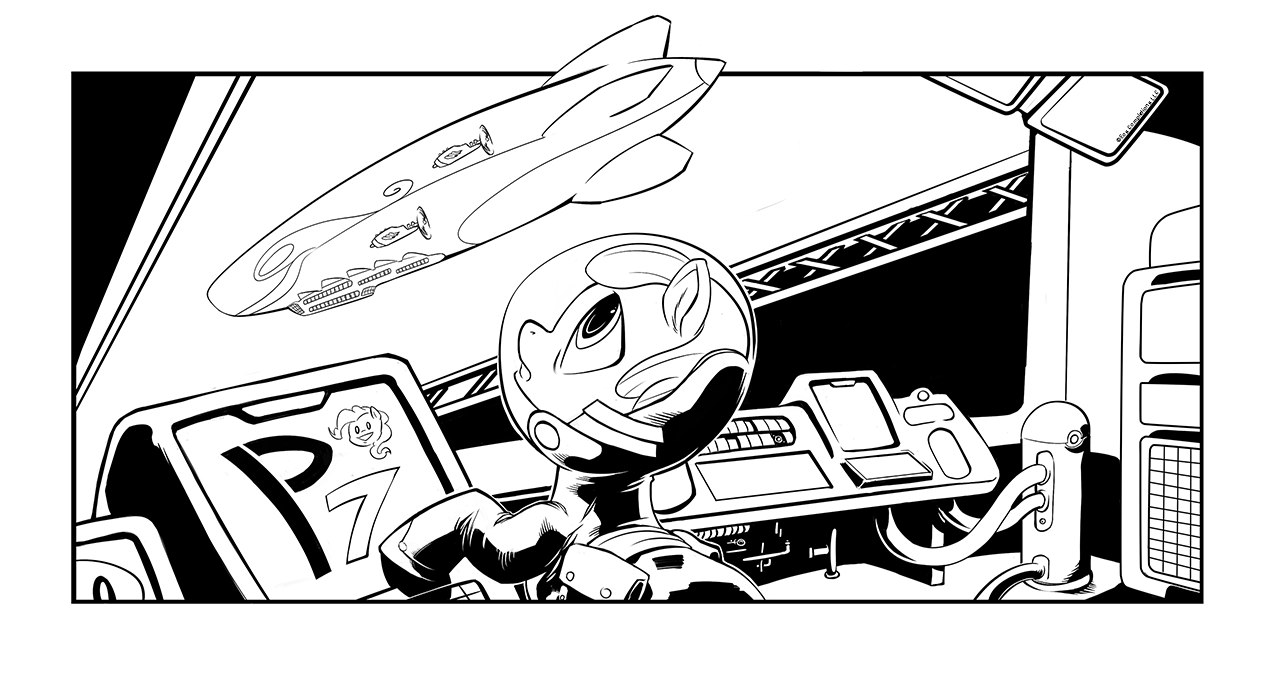
\includegraphics[width=\linewidth]{image04.png}


\begin{intro}
知道吗?你们是我最好的朋友\footnote{MLP动画片头曲最后一句}!
\end{intro}

\daytimeplace{4}{3:15 PM}{炫彩大厅,盐块城}{The Glow, Salt Cube City}

「这不可能的!尸鬼是超级笨笨的吃小马僵尸!你们虽然有点丑但是你们是好马,你们肯定不是尸鬼!如果你们不告诉我尸鬼在哪,那我自己找去!哼!」帕比吐舌头。

软气和桃花相互对视了一下,然后桃花说:「我们没必要说谎啊,帕比。我们确实是尸鬼,并不是每个尸鬼都是没脑子的食马族。」

「但是他们和我说……」

「你耳朵里从来就只听你想听的话!老天啊,你是我见过最闹心的熊孩子,没有别的马这样说过你么?」桃花叹了口气,这孩子简直是选择性信息接收的典型。「醒醒吧,幽灵!这里可不是什么……充满魔法的神奇大陆,这里是小马国,没有比这里更烂的地方了!」

「但……但是……」帕比后退了一步,不知道是那个腐烂的小马,还是她现实得不能再现实的语言吓到了她。

桃花往前走一步,蹄子重重跺在地上。「别扮你的天真幼驹了!你和我们一样是怪物!别装了!行不行!?」

小雌驹吓得一屁股坐在地上,抱着脑袋把脸缩进了自己的前蹄之间。「别,别这样,我会做个乖孩子。」

「我才不需要你做乖孩子!你醒醒好么!」桃花在地上跺一把蹄子。

软气拍拍桃花的肩膀安抚道:「冷静一点桃花,我不觉得她在装模作样,冲动是魔鬼啊……」

尸鬼雌驹推开他的蹄子叫道:「她已经两百多岁了,两百多岁啊!怎么可能还这么天真?!她是智障吗?!我觉得她就是在耍我们!我们应该……」

桃子的话被一阵可怕的哭号声打断了,那一瞬间她似乎回到了自己的童年,\emph{那一天她把自己不小心锁进了衣柜,一直到日落之前都没有马来找她,那种孤独,被遗忘的恐惧让她拼命大叫,那天她几乎叫破了自己的嗓子都没有谁来救她}。在这令她窒息的罪恶感之中,桃子意识到帕比并没有耍他们。

所有的尸鬼转头看着那个黄色的小幼驹,她的哭号声之中似乎有着几分不自然,就好像是某种梦魇让营地里面的所有小马都感觉脊背一凉,或许这是因为那个愤怒的尸鬼在几个世纪以来第一次听到幼驹的哭声,沙盒微微迟疑了一下,然后轻轻抱起她。

「她……她到底是什么?那声音……」桃花吃惊得几乎站不稳。

「这下你把她弄哭了!」软气平铺直叙的语气说:「这回你让她相信我们是坏蛋了,干得好。」

「我勒个去,你们能不能让她别哭了?!」一只带着橙色头盔的小马抱怨着:「吵得我头都大了!」

沙盒抱着幼驹,一直到她的哭声变成低声啜泣。「好了好了,我知道你是个乖孩子,没关系的,你只是想妈妈了。」尸鬼首领搂着帕比说:「不管是谁都有脾气不好的时候,桃花姐姐很不开心,所以你道个歉她就能原谅你,不过下一次她和你解释什么事情的时候,你可以仔细听她讲话吗?」

帕比慢慢点了点头,看着沙盒那成熟的双眸,稍微找回一些宽慰。然后幼驹转头看着雌驹低下头。「我……我很抱歉没相信你说的话……桃花小姐,我现在知道你是尸鬼了,我错了。」

这个道歉让桃花的负罪感更深了,不过既然谈话现在有点进展了她也只能忍了。

「没关系小家伙,长辈说话的时候稍微注意点就好。」她顿了顿,刚刚说到哪里了「呃,我想你提到想要我们走开?为啥?」

是不是早就说过小孩子很容易分心?

小幼驹现在正挠着头盔想着这个新问题,但是却想不出一个答案。「我想……是因为那些漂漂马答应如果我来这里看看情况然后回去报告,他们就让我骑上双头牛兜风。他们似乎说过如果尸鬼都不见了就太好了。」帕比又想了想,似乎想要记起整个故事。「虽然我说已经长大了可以嘘走一两个尸鬼,但是他们还是让我发誓只是进来看看,不过因为我说的时候交叉着蹄子所以这个誓言不算数。」幼驹开心的笑着,自豪地挺起小胸脯。「我比他们聪明多了!」

软气听了笑出声来。

「赛蕾斯蒂娅哦,这个小雌驹真讨喜,我们能养她么?」

沙盒叹了口气。

「这还真是个……巧合,桃花,去找好好博士,我有几件事想和她说。软气,你能帮我看着她么?去我办公室把那个粉色玩具给这个小客人。」

\horizonline

\daytimeplace{4}{4:00 PM}{炫彩大厅,盐块城}{The Glow, Salt Cube City}

帕比爱死她的新萍琪派布偶了,一直紧紧地抱着它,时不时地秀给身边的马看。可惜在她身边的基本上只有软气。

「看到了吗?她超酷,比那杀马的机器萍琪好一百倍!而且超软!」黄色的幼驹用蹄子揉着布娃娃说:「太空服讨厌死啦!我想要亲亲它都不行!我给它起名字『丝尾』。」

「我说,小太空马,看这个!」软气敲了敲帕比的头盔说,然后举起一盘全息磁。「你猜猜这是啥?」

帕比歪着头,「呃……这个……黑色的?我知道了,是那个什么什么的什么什么!」

「我就知道,好了天才雌驹,过来让我把这个接上你的外衣。」尸鬼抬起帕比的左蹄然后打开前臂上的一个接口,把那个磁带插进去。

「{\mt 备份发现,读取中。警告,系统运行在应急模式,无法进行复制。备份拷贝结束。当系统运行正常后会打开文件。}」

「嗨,声音先生!」帕比打了招呼但是却没有得到回音。「我不知道怎么回事,好像惹声音先生不高兴了,我一来这里他就闷不吭声。」

「别担心,只是因为『盐块』,那东西影响了普通魔法晶片。」软气看着幼驹的表情笑了笑,她看起来好像在仔细听你说话,但是实际上一个字都没听进去。「那东西让声音先生打瞌睡,你们俩离开炫彩大厅之后他就醒了。」

帕比点了点头,「别告诉其他小马,我一直觉得有点寂寞……我不是说我没有朋友,而是最近几天好像一直没有马想陪我……所以……」帕比低下了头,「声音先生虽然有点笨笨的,又老是说些不知道什么意思的话,还经常发脾气,但是他从来不离开我……我只是希望他没生气。」

软气想说两句话安慰她,但是却被另外两个小马的争吵打断了。

「我们没那时间了!链式反应已经在加速了,你难道看不到吗?这东西已经变成青色了!」他听见沙盒的声音从门里传来。

「我没瞎,但是我觉得你疯了!我们还需要好几天,并不是你想的那么简单……打开圆顶然后吹起气球说拜拜!我需要时间初始化系统,然后给自动驾驶系统编程输入航线。至少要两天,不眠不休也要至少三十小时!」这是另一个雌驹的声音。

「它最多只能再坚持七八个小时了!如果我们再等下去就来不及了。」

「我真奇怪为啥这东西变化得这么快,这个破盐块在圆顶建成之前就蹲在这里了,然后现在你告诉我末日倒计时还剩下七个小时?」

帕比转头看向他们问:「发生什么事情了?」

「我不清楚,小家伙。」软气皱起眉头,这可不是什么好消息,而且也没法和她解释,就算和她解释清楚也只能让让她更惊慌。于是他说:「嘿,你想看看北边大厅的礼品店么?」

\horizonline

\daytimeplace{4}{4:45 PM}{炫彩大厅,盐块城}{The Glow, Salt Cube City}

「……这就是小马国成立的故事!」帕比说。

「啊,没错……还真是个神奇的故事,但是我刚刚想问你,你之前说的那个提问者是谁啊?」

「你说那个故事?算啦,无聊死了!我还是讲那次我不小心吃了一个蝴蝶的故事。」

软气低下了头,小声的说:「那天我在街上跑的时候,看到一个超超超超超级漂漂的……」

同时帕比也一边蹦跶着一边说:「那天我在街上跑的时候,看到一个超超超超超级漂漂的……」

\horizonline

\daytimeplace{4}{5:15 PM}{炫彩大厅,盐块城}{The Glow, Salt Cube City}

沙盒从礼品店门口探进头来,看到帕比和终于松了一口气的软气。「你们在这啊,别跑这么远,这里可能会有野生尸鬼。」

软气笑了:「别担心,我们的神奇小丫头能解决一切。」

沙盒歪了歪头:「你是说,她还被尸鬼袭击过?」

「当然,之前有那么一次,我要说这个小家伙完全能应对自如。」

「那最好,」沙盒叹了口气,「因为我真的很需要她帮忙!」

「嗨,丑丑马老大!」帕比带着开心的微笑跳到尸鬼首领面前。「我喜欢这个地方!我有个超棒的主意!我可以去告诉城里的小马,所有的『尸龟』都跑掉了,然后他们就不会来烦你们了!我们可以给你们找点漂漂衣服……然后把你们打扮成……呃……没那么丑的小马,然后改个名字,比如说鸢尾什么的!这主意超赞对吧?哦,对哦,你还需要一把长号!」

沙盒露出了微笑,那笑容有些悲伤。「我还真想试试看,不过很可惜,我是来告诉你我们要离开这里的。」

帕比的耳朵耷拉下去了:「你们真的要走?但……但是你们不能走啊!这里是你们家,而且你们又不是坏蛋,为什么要走?」帕比着急地踱着步,「等等,我还有个主意!我们可以给其他小马一个超级好的礼物,然后给他们办个派对告诉他们你们不是邪恶的!绝对可以的,绝对绝对可以的!」

沙盒叹息着用蹄子拍着帕比的头盔:「别绞尽你的小小脑汁了,这不是你的错,只是一些该做的事情,而且我需要你的帮忙才能做到。」

「沙盒,你能跟我解释一下到底发生了什么吗?我听你和好好说FFO的燃料什么的,是和我们回来的时候你们说的那件事情有关么?」

沙盒推了推他的眼镜回答:「没错,我们早知道盐块不稳定了,这么多年以来它一直以一种固定模式吸收着超聚魔法的放射线,就像我说的,在几个月之前这个模式忽然加速了,这个反应已经无法逆转,它距离完全释放能量还有不到五个小时了。」

软气沉下了脸:「好吧,这么说我们确实没多少时间了,那么怎么办?我看友谊一号 (Friend Force One) 还需要点维护工作,你确定这个完全释放啥的靠谱么?会释放什么?」尸鬼已经知道答案是什么了,但是他还抱着一丝希望。

「我不太清楚,可能会是比最大的斑马超聚魔法弹头还要大好几倍的魔法冲击波。那导弹打到这里的时候,这个大号盐块里面的魔法回路可不是设计用来对抗超聚魔法的,它已经尽它最大努力把盐块城的死亡宣判延迟了这么久。」

帕比想要听他们说什么,但是对话内容从一开始就听不懂了,那些花里胡哨的词汇让她觉得头晕,她甚至怀疑语言里面根本不可能有那些词。所以她决定自己去圆顶的其它地方看看。

软气伸出蹄子按住了帕比的头盔,还没等她出门就把她安稳地留了下来,老实呆在身边。

「现在FFO的导航系统还没校准,而且自动驾驶也不工作。」

「没错,不过我也没指望那东西,我要亲自飞那艘船。」

软气说话时嘴几乎是颤抖着的:「你开玩笑吧?这是自杀!而且你也不可能独自飞那东西,引擎室和氢气发生机都需要有马看着。」软气看着帕比,然后露出惊恐的表情。「难道你想让她……」

「不,别担心,她只是我们出去的门票——MK VI防护服的A.I.回路用的是和P7计划一样的东西,她只要站在里面就可以自动操作控制室。这能给我们节约很多时间。」沙盒说:「你真觉得我会把她带上么?」

「你听我说,我们其实只要撤离这个鬼地方,然后让那个盐块把苹果塔的那帮混蛋炸上天就好,我们什么都不欠他们。而且我们一出圆顶他们就开枪打我们,不是吗!我们从地道跑掉,然后让这帮家伙尝尝这个马芬的滋味。」

沙盒直视着软气的眼睛,「你想做什么做什么,我只是想让帕比去帮我打开屋顶好让我起飞,我不管我能飞多远,但是我不想再让任何一个孩子因为我不作为而死掉,我知道你恨白苹果塔那些小马,但是你难道忘记了城里的无辜妇女儿童了么?难道她们就应该当你仇恨的牺牲品?」

帕比还是想要跑,顶着软气的蹄子拼命刨着蹄子。「让我走啦,我要去外面玩啦!」

软气看着帕比,如此的天真,她甚至完全没有意识到她现在面临的灾难,就算告诉她能跑多远跑多远也没有用,如果那个超聚魔法爆炸的话……

「我去看看引擎,你告诉我该怎么做就好。」

沙盒点了点头,「我知道我可以信任你,桃花也要去,好好已经在舰桥了,我现在去教帕比该怎么做,估计要花一点时间。」尸鬼低头看着黄色的幼驹,「嘿小家伙,想去一个新地方探险么?」

\horizonline

\daytimeplace{4}{6:30 PM}{炫彩大厅,盐块城}{The Glow, Salt Cube City}

\emph{「再重复一次,宝贝。」}

\emph{「妈咪,我已经说了一亿次了!」}

\emph{「再说一次就好,这是一个超级特别的秘密咒语,你必须一点不错地说出来才能有用,帮妈妈个忙,好么?」}

\emph{「那么一会儿我能吃马芬吗?」}

\emph{「快要吃午餐了,如果你吃马芬的话,你也要吃苜蓿哦。」}

\emph{「这不公平,你总是给我一大堆那东西!」}

\emph{「我还会给你个超级无敌抱抱亲。」}

\emph{「呃……那好吧,当我在那个大圆门前面的时候,我应该把蹄子放在绿色按钮上。」}

\emph{「很好。」}

\emph{「然后那东西就会问我什么什么识辨码。然后我应该说……呃,可以提示提示我吗。」}

\emph{「你肯定记得,稍微仔细想想,妈咪知道你是个超级漂亮聪明的孩子。」}

{\mt 「请说出您的身份识别码。」}

「\dots FT\dots 0\dots 0\dots 1\dots 6\dots 5\dots RD\dots C\dots 1\dots G\dots A」

\emph{「对了,看吧,超简单,我就知道你能做到,然后呢?」}

\emph{「然后会问我另一个什么码?}

{\mt 「请说出该ID的密码。」}

\emph{「然后你应该说……」}

「嗨,我是快乐帕比!」

{\mt 「ID接受,首席技术官阴雨·黛丝。允许进入控制室。警告,这里有三千六百九十八个错误信息需要处理。」}

\emph{「记住哦,如果你听到很大的喇叭声,你就要马上跑到这个秘密地方,然后用我给你的咒语,不要等我,懂了么?」}

\emph{「懂了,妈妈!」}

\emph{「我爱你帕比,过来让我抱抱……」}

这里虽然不是妈妈告诉帕比应该去的地方,不过那天听到很大的喇叭声的时候,大家都跑到外面玩去了,帕比不想自己一个人去地下……不管怎么说,这个咒语对这个门也有用。或许这个就是『芝麻开门』?

在门后面是一个超级大的房间,有很多闪亮的面板,远处的墙实际上是一大块玻璃,上面都是蜘蛛网一样的裂痕。帕比走进屋子的时候,门就在她身后关上。

「{\mt 警告,侦测到中等辐射,威胁级别:可忽略。所有系统,启动。}」

「声音先生你又回来了!我正想说……」

「{\mt 全系统工作正常,检测到通信连接请求,认证源地址。认证完毕:士气部建筑ID00201——盐块城圆顶控制室。交换通信协议……完成。警告,该防护服系统版本过于老旧。升级中,请稍候。}」

「哇哦,你还真能说,你是不是想我了!我超想你,我找到了那些要找的尸鬼了,但是他们不是坏蛋!而且他们很和善,就是有点丑……桃花训斥了我,不过的确是我的不好,所以我说对不起他们说没关系!然后软气给我一个……」

忽然一个叮叮声打断了帕比,她站在原地愣了一下之后马上去找那个有趣声音的来源。在蹦蹦跳跳一会之后,她看到在一个脏兮兮的桌子上放着一个红色的电话。帕比接起了话筒。

「您好,妈妈不在这里,我是个小孩子所以没办法做记录,您可以在晚餐的时候打来么,超超超拜托?」

「帕比,是我,沙盒。」一个熟悉的声音从电话里面传来。「看来我的黑客工具有效了,你现在也在控制室内。现在我们仍然需要点时间更换电池然后充入氢气。所以你务必要呆在那里。」

帕比看了一眼沙盒之前给她的小盒子,然后回答:「哎呀!我忘了!我没用它!」

「那你怎么……算了,没关系,仔细听好,我先要把电话关了,等我们准备好会再打过来,所以别碰任何东西,好么?」

「好的好滴好得!拜拜!」帕比把话筒放下,整个地方看起来到处都是灰土,让帕比想起那个破掉的大圆门里面,不过这里小很多,而且有很多桌子和屏幕,不过大多数都坏了。

忽然一盏红灯在坏掉的大窗户前亮起来,紧接着,更多的红灯亮起,这次几乎每张桌子上都有。几个屏幕开始闪烁着绿光。把帕比吓得一屁股坐在了地上,有点不知所措。「我可什么都没碰,对天发誓!」

「{\mt 升级完毕。P7基本客户端安装完毕,系统重启。}」

忽然整个衣服都变暗了,帕比又一次体验到了在中心城醒来那天的麻痹感觉,不过这次只持续了几秒。

「呃,这感觉好好玩……」

在帕比面前头盔的HUD上,出现一个有着七个气球的亮粉色标志,然后那个标志消失了,开始显示出普通的界面,除了顶部的罗盘以外,左右还有一大堆没用的东西,不过让帕比惊讶的是声音——不是声音先生,而是一个尖嗓子,而且听起来很友好的雌驹声音。

「嗨~!黛丝女士!我们这里有点小麻烦,所有的显示屏基本都挂了,然后我们损失了大概……100\%的职员。他们已经有多久没来上班了?哇哦……真的好久了!大佬们是不是该考虑提高一下员工福利了……哦哦,别担心!我可以在你的个人终端上操作所有东西。」

「呃,你是谁啊?声音先生去哪了?」

「我是萍琪七号!你最好的朋友,最好的小马--机器交互界面!而且我的安全程序已经写入了『不准尝试统治世界或者变成机器神明』!我很棒吧,不是吗?」

帕比挠了挠头盔,然后问:「你认识机器萍琪么?」

「哦,那当然!我们都是整个系列最先进的!她正在用于测试……呃,等等,那个测试几天之前已经完成了,我们看看结果……好像说那个测试派对实在太棒,每一个小马都爱死了!呃……不对……是真的死了么?……听起来一点都不好……好吧,我们别再提这个机器萍琪计划了,好不好,好不好?」

「但是她伤害了很多漂漂小马。」

「资料删除中……已删除,我很抱歉,我不知道你在说啥。还有其它事情么?」

「呃……机器萍琪?」帕比又问。

「没听过,还有什么事情么?」

「啊……对了,还有要飞……什么东西……」帕比戳着头盔努力在回忆。「声音先生哪里去了?我更喜欢他……」

「你……不喜欢我吗?你不做我的朋友吗?但是……为什么啊?我已经这么努力了!我已经在这里等了……大概……两个世纪啦!拜托别把我丢回服务器好么!那里又黑又孤独,我只能在那里数这里的机器做了多少次循环!拜托啊啊啊!」

「呃……如果你保证你不绑架小孩的话……」

「不会,这种事情在我的程序里面绝对被禁止了,别担心,不会有绑票!不会有大屠杀!不会有末日审判!只是帮你完成日常工作,绝对绝对不要担心!而且……我还是要说,那些安全协议真心烦死我了!」

帕比咯咯笑着:「呦呵,声音小姐也会说听起来好厉害的话!」

「没错,有时候我也……对哦,你是首席技师黛丝女士么?因为你刚才说你的名字是帕比什么的。」

「笨笨声音!我就是快乐帕比!」

「哦……棒极了,正好是我喜欢的!入侵者!在落满灰尘的魔法回路里面呆了两百年之后,终于可以玩消灭入侵者的游戏了!」声音顿了顿又说:「帕比小姐,你并没有进入这里的资格,所以我必须请你离开,虽然说你不知道这件事情有多让我伤心!」

「但……但是沙盒先生说我必须呆在这里,不然友谊飞船就飞不起来!我能再呆一会吗,拜托,超超拜托,漂漂拜托?」

「如果你想呆在这里的话,你必须证明你至少是个军队的上校或者士官什么的,我真的……真的……真的很想让你陪我,但是我必须秉公无私!除非我有什么事情在忙,比如说一个逻辑悖论或者有趣的死循环\footnote{逻辑悖论与死循环:许多科幻小说中弄坏人工智能的惯用桥段}什么的……哦,等等!你和首席技师是什么关系?」

「谁?」

「阴雨·黛丝!」

「哦,她是我妈妈!你知道她在哪里吗?」

「不知道,但是这解决了大问题,让我看看啊,把这个弄到这里,这个到这里这个这个……妥了!今天是带女儿参观工作场所日!你开心吗?」

「呃……我想要妈妈。」

「喏,你看,这个事情都写在你的任务清单里面!你真的想要找你妈妈,是吧!」

「那当然,那是我妈妈!」帕比板起脸。

「你跟我说,我们可以……哦哦哦,等等,紧急路线有一个电话!」

沙盒的声音代替了那个A.I.的声音。

「帕比我们准备完了,你那边如何?」

「嗨,老大,我当然没问题,这个声音小姐真能聊。」

「真棒,现在仔细听好,有几个小马想和你道个别,乖乖听着,不会有多长时间,毕竟我们有点迟了。」

沙盒的声音又被桃花代替。

「喂,小家伙,你在吗?」

「嗨,桃花小姐。」

「我很高兴听到你的声音,我想说……对不起,我其实没必要训斥你……我们可以和好吗?」

「呃……没关系?」

尸鬼雌驹长舒一口气:「感谢赛蕾斯蒂娅,心里放着这事,我什么也干不了,请记住我的话,帕比,小马国是个不可原谅的地方,你必须相信你的朋友,因为在这里你很难交到朋友。我……我很后悔我们没时间相互加深理解,但是只要知道你很安全的话,我想我也就无怨无悔了。」

「你要走吗?你到那边之后我能去见你吗,好吗?我们可以开一个派对!」

桃花沉默了一会,然后回答:「可以……可以的帕比!如果我们有缘再见的话,我们会开一个超级大的派……抱歉,我离开一会儿……」

电话沉默一会之后,另一个声音响了起来,「嘿,帕比,我是软气,请听从沙盒指示哦,我们全看你的了!」

「软气!声音先生现在变声音小姐了,你说有趣不有趣?」

「你在说什么……算了,没关系,我想和你说件事情!我认识你的妈妈,不过别惊慌,我时间不多,你仔细听好。」

「你……你为啥不早和我说啊!」

「我想……我想早点说,但是这个超聚魔法让我忙得晕头转向,你现在听我说,我曾经是她的手下,第三装甲师『铁壁』的三等技术士官软气。你记得我给你的那个磁带吗?」

「呃……那个黑色的那个什么什么的什么什么?」帕比努力回忆着。

「对,就是那个,那里有我们长官的位置,大概就在盐块城南边,在沼泽那里,如果你想找到长官线索的话,那边一定有。所以在你把控制室的事情弄完之后,把165战指设为主要目标,然后跟着粉色箭头就好,你明白了么!」

「我……嗯,明白了,去指挥部,找妈妈!谢谢你软气,你是最棒的小马!」

「我想你是在说『萍琪派』吧。」P7打岔。

「还有最后一件事,帕比,你的旅途之中一定会知道一些让你伤心的事情,那是不可避免的,但是我知道你是个勇敢的孩子……所以,拜托,别忘记超聚魔法落下之前的那些日子,小马国现在是一片荒芜的死亡大陆,但是你知道这里不可能永远像这样荒芜下去!不要让废土侵蚀你内心深处的纯真!我会在太阳照耀天空之前一直看着你的!」

「呃……为什么大家都说这些伤心难懂的话?你们只是去坐个小飞机,又不是我们永远见不到了,我和妈妈会在你们找到新家之后再去看你们的。」

「帕比,这里是沙盒,你还在听我么?」尸鬼长者的声音打断了对话。

「啊……是的老大……你说,我们还会再见面吧,对吧?」

在一阵长长的沉默之后,尸鬼平静而又悲伤的声音说:「我相信,我们会在彼岸的尽头再一次相聚,如果你想再见面的话,请不要失去希望,帕比。」在另一阵沉默之后,尸鬼长官又开始说:「我们需要你打开屋顶好让我们起飞。现在,你重复我的话:『启动语音控制,授权码SB01,首席研究员,密码:阿加莎。改写协议01-11的优先权……』」

\horizonline

\daytimeplace{4}{7:30 PM}{闹市区,盐块城}{Downtown, Salt Cube City}

灌木正坐在窗户边用狙击步枪守卫着圆顶方向,他已经值班很久了,而且天色渐渐变暗,再过一个小时他就要挪窝下去了,希望下面能有一碗热燕麦粥等他。

「我很好奇为什么他们送那个小丫头自己去圆顶……她连午餐都没吃就进去了。可怜的小家伙,我们现在都开始让孩子去送死了……」小马一边启动瞄准镜的夜视功能一边喃喃自语。

就在那个时候,圆顶东边还完好的部分随着一阵金属的摩擦声开始坍塌下来。

「露娜我娘亲哦!那里怎么了?」卫兵用瞄准镜看着那里发生了什么。

在观察几分钟之后,士官确定房顶并不是真的在坍塌,不完全是,那里的确有很多灰尘和零件落下来,但是建筑的东边实际上是在……旋转?经过两百年的风吹雨淋,整个圆顶早就快锈成一块铁疙瘩了。但是现在有什么巨大的力量正扯开那些不想动的铁板。在被轰炸那天之后就被忘记的钢铁老古董在一阵金属哀嚎声中裂成好几块。

不管怎么说,房顶依然慢慢移动着,虽然对自己的结构造成巨大伤害,但仍然旋转开来。现在那堆垃圾的最后一片也消失了,『圆顶』完全滑到了一边,露出一个像城镇广场那么大的空间。

那个噪音让闹市区的所有小马都抬起了头,有些雌驹当场就吓昏了过去,倒下前还大叫着「好可怕,好可怕\footnote{好可怕好可怕 (The horror! The horror!):\emph{MLP} 动画里面鲜花三姐妹吓得满街跑时的惯用语}!」之类的话,但是不为所动的士官依然冷静地举枪瞄准那个大洞。

「好了,尸鬼,让我们看看你们腐烂的脑袋里面装了什么。」

在房顶一阵金属摩擦声中停止移动的同时,另一半房顶也停了下来。然后整个天空被数千盏粉色的探照灯照得一片明亮,随着又一阵蓝色和绿色的烟雾和亮片从圆顶周围喷上天空,一个尖嗓子的声音开始喊话了。

「女士们,先生们!」声音从圆顶的喇叭里面传出来,虽然带了很多杂音,而且一个喇叭似乎坏了。

「为我们伟大的赛蕾斯蒂娅公主和露娜公主献上我们最诚挚的敬意!我在这里心中满怀荣耀地向你们介绍我们最尖端,最神奇的最新大型交通工具!『友谊一号』!她让小马国交通更加便利!」

然后是一阵音乐声。

「现在让我们介绍嘉宾!首席技师黛丝女士的女儿,快乐帕比!」

「……然后我说道:『燕麦粥,你疯了么?』接着是一阵沉默。呃……那是我的声音么?啦啦啦啦啦啦~!呀,真的是!太有趣了,再见尸鬼们,祝你们旅途愉快,给我寄明信片哦!」

士官灌木抬起了眉毛,「到底发生什么了,首席什么黛?谁是黛丝女士?而且那个……我……去……是……什么?」

在打开的圆顶中,一个形状奇怪的东西慢慢升了起来,它看起来像是一个气球,但是却非常长,看起来像是一根尾巴很粗的巨大玉米棒,在两边还写着『友谊是魔法』的大字。

士官揉了揉眼睛,把自己掉下来的下巴用蹄子合上,现在那艘飞空艇已经从圆顶升了起来,然后慢慢转向,在那个粉色的巨型气球下面是一个类似天空马车\footnote{天空马车 (Airwagon):\emph{FoE} 设定中天马可以拉着飞的马车,可以靠天马的魔力悬浮在空中}的东西,但是大好几倍,在身边伸出的两片鱼鳍一样的翅膀,后面还有好几个螺旋桨。

然后这东西开始加速,避开塔尖,朝东南方向飞去。士官满脸难以置信地看着那气球飞走,那个尖嗓子声音还在喊着。

「非常好,这是士气部给你们带来的表演,大家,记得买战争基金哦!而且记住,你们不开心萍琪派也不会开心!所以微笑吧!因为她会永远注视着你们,永远永远哦!」

当圆顶的灯光和音乐都消失的时候,气球已经飞了快一公里远了。圆顶想要再关上,但是却只是带出一阵新的金属摩擦声,然后变成了一堆碎片。

「我勒……个……大……公主……啊……他们……他们……就这么……坐上那东西……跑了?」卫兵挠着头,「为什么早不走?而且他们从哪儿弄来那滑稽的东西?友谊是魔法?简直疯了!」

\horizonline

大概一个半小时之后,小马们都回去睡觉了,飞空艇也成了远处天空的小点,早已经在几十公里外了,不过比起天空马车来说真的飞得不快,不过它非常大。

楼梯上传来的马蹄的声音让灌木士官警觉地竖起耳朵,不过他的视线还在飞走的气球上。

一只穿着战斗鞍具的雌驹敲了敲墙,然后走进屋子。「该换班了,伙计,刚才是不是很精彩。」

卫兵转头看着他的战友。「他们……就那么飞走了?那么大一气球……我不明白,为啥要飞走?」

雌驹看着外面,然后问道:「喂,你没觉得少了点什么吗?」

「对,尸鬼和剩下的圆顶屋顶都不见了。」

「不,我不是想说这个,你看,那炫光也不见了。」

「哎呦我去!你还真说对了,圆顶不发光了!看起来黑黑的……闹鬼一样,真有点毛骨悚然的……」

「所以,他们真的走了?明天早上天亮之后我们去检查一下辐射剂量。」

「你觉得……」忽然整个世界都被漂白了。炫目的光芒让士官睁不开眼睛,他一直到光亮消失之后才看清发生了……

轰隆!

这是他听过最大的声音,就像暴风之中的惊雷一般,而且更大声。卫兵立刻抓着他的战友卧倒在墙后面。

下一瞬间强大的震动和一堵烟尘的巨墙袭击了闹市区,把无数窝棚都弄成碎片,只剩下几个坚固的建筑。

「那……那是什么?」士官拼命想睁开眼睛。

「我不知道……尸鬼的飞天机器爆炸了?看起来像是什么巨大的……」然后雌驹意识到了那是什么。「哦我的赛拉丝蒂亚啊!是超聚魔法!他们飞的那东西上带着一颗核弹头!」

~\vfill

\begin{note}
    升级Lv 3

    新专长解锁:应急训练——魅力($7 \to 8$)现在你比之前要酷了14.28\%!
\end{note}



\chapter{小鸡}

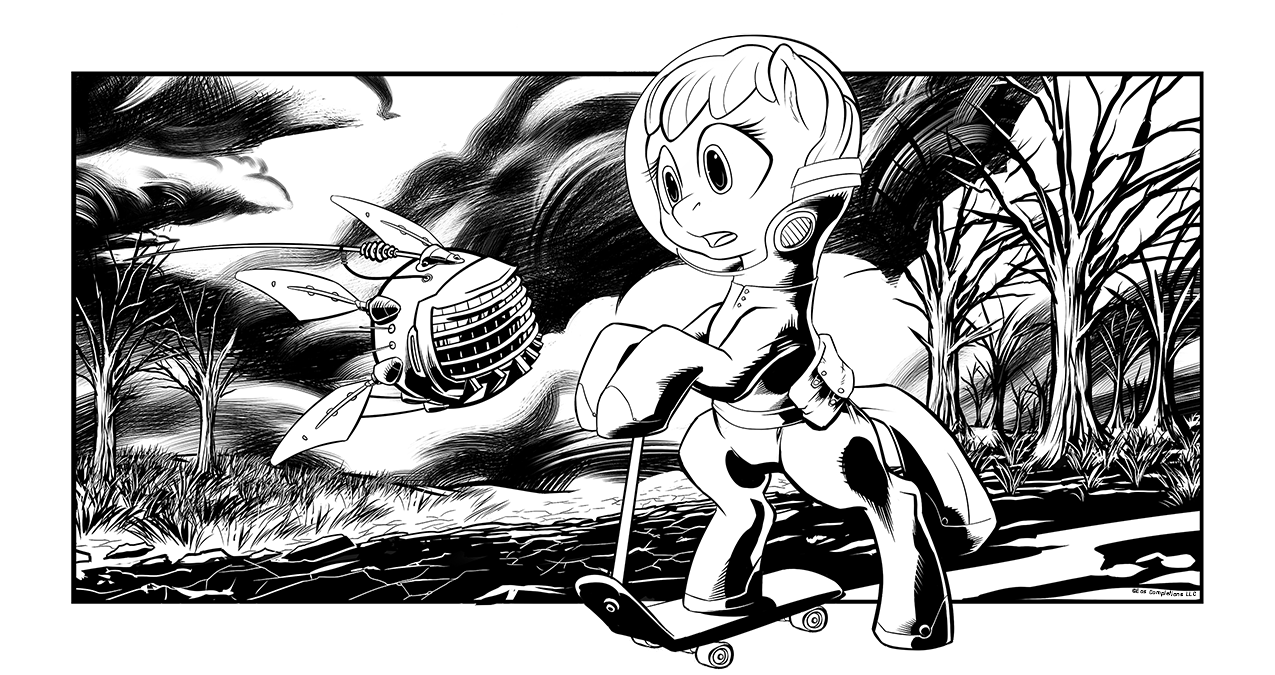
\includegraphics[width=0.9\linewidth]{image05.png}

\begin{intro}
可爱标记童子军小鸡营救队来了!
\end{intro}

\daytimeplace{5}{9:30 AM}{闹市区,盐块城}{Downtown, Salt Cube City}

「耶!漂漂牛快点!再快点!」

双头牛左边那个脑袋重重叹了口气,然后一脸绝望地望向旁边带着黑帽子的独角兽。

那小马对牛无奈地笑了笑,挥着蹄子打断她无声的抱怨:「这是交易的一部分,别不满意啦,再让这个幼驹骑最后一圈,然后带她来我办公室。」

「好,好,白先生。」牛不爽地在白塔外面转来转去,在之前的半小时她们已经跑了好几圈了。虽然外面的小马都在忙着修理昨晚冲击波造成的破坏,但是被一个黄色小雌驹骑着还是会引来很多好奇的目光和窃窃私语。

「我认得她,是嘉年华的幽灵……她诅咒了那些尸鬼,这个孩子一定会带来厄运……」

「你看,她在白塔外面装傻,我敢用我的所有瓶盖打赌,她一定用她在圆顶里面看到的东西来威胁他们呢!」

「你没看到吗?圆顶的炫彩已经消失了,然后……然后尸鬼的飞船也爆炸了!他们肯定想搞什么鬼,结果反而坑了自己。可恶的尸鬼,他们就是活该!」

「但是……她到底是谁?」

「别问,我从来没看见她吃过东西,甚至没看见她打开自己的头盔,虽然不知道怎么回事,不过她绝对不是好东西。」

「别说了,她过来了!」

帕比自己玩得很开心,完全没有去留意那些窃窃私语,「太棒了,超超超有趣,牛小姐们,我们有时间再玩一次好吗?」

双头牛的其中一个脑袋点了点头,「当然,不过你要先问问白先生,他在办公室等你,就在红色的门里面。」而另一个头一脸不爽地继续反刍着。

白先生的办公室很大,很整洁,墙上挂了很多照片,而地板亮得可以照见自己的影子。

「哇哇哇!这个地方真的超超超漂漂!」

白苹果的老大是一只戴着黑帽子的雄性独角兽,毛皮是白色,鬃毛是天蓝色。「嗯,谢谢夸奖,黛丝小姐。」这个称呼似乎让帕比愣住了,所以白先生又说:「那个圆顶的声音昨晚不是说你妈妈是阴雨·黛丝吗,所以你的全名是快乐帕比·黛丝,是吧?」

帕比歪了歪头,最后又点了点头,「嗯,没错。现在我该走了……声音小姐在我的罗盘上显示了一个箭头,所以我该往那个方向走了。我可以走了吗?拜托。」

老白叹了口气,压低帽子挡住了他的眼睛。「当然,没问题……但是……我还是想问你最后一件事情。圆顶里面以前是什么东西在发光?」

「你是说盐块吗?」帕比就像听到什么有趣问题而咯咯笑起来。「你好笨哦,我是说,你不是一直住在盐块城嘛,你居然都不知道盐块,真是……」

那个老马正要大声训那个小雌驹,但是仔细想想和小孩子闹脾气又没什么用,所以他只是笑了笑。「我承认我一直没去过圆顶,那里有点……可怕,所以,是尸鬼把那个盐块带上他们的飞船了吗?」看着幼驹一脸迷茫,于是他补充道。「就是那能飞的气球。」

帕比点了点头。「没错!他们看起来超级着急的样子!他们都说会什么……盒爆?……核包……啥的?」帕比看起来不是很开心的样子,「反正是什么什么东西,我记不太清楚了,但是他们说他们要在发生之前走得远远的,因为很危险?」

「核爆?是这个吗?」

「对!他们说因为链啥反应……反正就是那个方块要赶紧丢得远远的,我还帮他们了!」

蓝色鬃毛的小马一脸惊讶,「他们……想要带着那炸弹走得越快越好?我……我知道那些尸鬼都是疯子,但是他们居然……好吧……我想这解释了为什么圆顶的光消失之后放射性几乎消失了。」

白先生露出放心的笑容,「你干得很好,小家伙,我很想再招待你一会儿,但是你这么急着走的话,至少让我送你出门。」

「好的好的!白先生!拜拜!我会告诉我妈妈你对我很好!」

「好,一路顺风小家伙,很抱歉我有些好奇,你想去哪?」

帕比指着南边说:「那里!妈咪就在箭头的终点!」

「哦,直接去沼泽地啊……祝你好运!」

她死定了。

这个沼泽是52号国道北边最危险最糟糕的区域。这个幼驹只会变成某个废土强盗的早餐。虽然很可惜浪费了这么好的防辐射服,但是白苹果家族不是强盗。

白先生沉思了一会,回忆着昨晚的事情,虽然这小姑娘就要走了,但是这样利用一个小孩子,让他后悔不已。她或许拯救了整个盐块城,但是他又给了这个孩子什么回报呢?只是骑着牛跑两圈?她就要遭遇危险了,而他甚至连一点建议都没有?这太不公平了。

「喂!黛丝小姐!等一等!我有东西送给你!」

\horizonline

\daytimeplace{5}{11:30 AM}{盐块城外,52号国道北部}{Salt Cube City Outskirts, Big 52 N Branch}

「呀……呵……!」一颗踩着红色滑板车的黄色子弹飞驰在公路上。

盐块城的建筑早已远远甩在脑后,路边的景象又变成了一片荒芜的废弃农田。

% NOTE: 遵照英文发布版改

\rcpr{仔细听我说,你到了乐麦镇之后,就绕道,穿过沼泽的路——}怎么怎么怎么怎么\rcpr{——一定要记住,绝不要穿过}什么什么什么……一些无聊的东西,帕比已经记不清了!

幼驹骑着滑板车嗖嗖地飞驰向南方,似乎是觉得滑板车的声音不够刺激,帕比还自己加上音效。「呜呜……嘟嘟……!飞向月球!宇宙无限!太空战士安德洛队长拯救世界!耶!」

在黄色幼驹面前,路上都是腐烂的田地和荒芜的农场,盯着箭头走了一会之后,农田变成了枯萎的果林和满是泥水的水坑。偶尔会有一两个营地,但是看起来已经遗弃很久了。虽然还有一点点生命迹象,但是都是一些昆虫或者不敢惹帕比的野兽。

唯一敢于接近帕比的,是一个飘在路中间的机器精灵。

「嘀嘀,我是吉普车!太空战士来啦!」帕比在玩疯的时候从来不会注意细节,黄色子弹继续以最高速度飞驰着。机械精灵在被撞上的前一瞬间连忙躲开,然后又急忙追着帕比飞。

「嗨,帕比,这么急着去哪儿啊?」一个熟悉的声音从喇叭里面传出来。

「提问者!我好想你!快看我的新滑板车!」帕比一边全速前进一边咯咯笑着,「我还认识另一个说话机器,不过那个很有趣,或许她不是一个机器?我不确定。」

「真有趣,可以和我讲吗?」机器精灵没等回答就接着问。「昨晚盐块城发生了什么?那个大爆炸是怎么回事,圆顶怎么了?你能停一下么,拜托!」

帕比叹了口气然后开始减速。「真会挑时候,人家正玩得开心呢……」

停下来之后,幼驹跳下滑板车,她一边想着守望者的问题,一边敲着头盔下面下巴的位置。「你是问圆顶?我在那里交了好多朋友!老大沙盒,软气先生,桃花小姐……哦哦,还有声音小姐!」

「不是声音先生了?」

「不对,傻机器,有一个声音先生,还有一个声音小姐!她住在圆顶但是声音先生可以随时叫她来,她超级酷而且帮我给尸鬼们办了一个送别派对!」

「哦,另一个小马--机器智能交互界面么……那么……你见到了尸鬼,还办了一个送别派对?你是什么意思?你帮他们发射的飞船?」

「太对了!」帕比兴奋地点着头。「超超超超级棒!我从窗口看到一个大大大大的东西高高高高地飞上天!」帕比举起前蹄描述那东西飞得多高,但是举过头了让自己一屁股坐在了地上,她咯咯笑着坐正了继续说。「然后好多好多灯照得雪亮雪亮的!我听到我的声音超超超超级大,所以我说『啦啦啦……拜拜尸鬼』然后他们就飞走啦!超级酷!滑板酷!」

「滑板什么?」

「滑板酷!」

「有这说法吗?」

「当然滑板!」

「你知道么……显然那滑板对你的小脑袋没什么好处……」守望者的声音听起来有点担心,「好吧,扯远了,那爆炸是怎么回事?」

「什么爆炸?」帕比不解的歪着头。「你说房顶又塌了?」

「不是,我是……等等……又有房顶砸你脑袋上?」这句话很明显让守望者有些惊讶。

「没错,那个房顶打开,然后大气球飞走之后,整个地方嘎吱,然后咣当!正好掉我头上。」帕比咯咯笑着,「但是我是一个超级太空小马,所以我把自己挖出来了……我就是那么厉害!」幼驹自豪地笑着。

机器的喇叭里面传出一阵笑声,然后又是一个叹息。「好吧,现在你要去哪儿?」

「当然是下一个妈妈地点!很明显,第三次会交好运!」

乒!乒!

忽然一阵枪声在空中响过,不过子弹明显不是向着帕比或者守望者来的,但是幼驹很明显听到了声音。「那是啥?」

「我……很抱歉帕比,我该走了,附近可能有强盗,你最好躲起来等他们火拼结束。」

「火烧?哪有?我要吃!」帕比蹦蹦跳跳地四处张望起来。

「塞拉斯蒂娅公主,请务必保佑她安全……」机器精灵的声音被一阵音乐代替之后,那个无人机飞走了。

声音是从帕比头上传来的,小幼驹抬头看的时候,看到令她难以置信的景象:有些超级大的飞天小马一边放着烟花一边飞来飞去,就像超华丽的芭蕾舞。这个场景让帕比回想起那天妈妈带她去飞行场看漂漂天马在天上做超级有趣的表演。

这次看起来也差不多,虽然有点不同的是飞在天上的小马不停地在闪光并且发出很大响声,帕比马上觉得这一定是他们最喜欢玩的娱乐项目。

但是她马上发现那些大家伙不是天马,所以幼驹皱着眉头问道:「我说,声音先生……那些小马生病了吗?」

「{\mtzh 分析中。友善的狮鹫。}」

虽然帕比一点都不明白狮鹫是什么,但是如果声音先生说那是『友善』,那么都可以啦。黄色幼驹挥着蹄子大喊起来。「喂!漂漂马!我在这里!喂喂!」

其中一个生物转头看了地面一眼,然后放松警惕的它马上就被另一个生物击中,然后打着转栽了下来。

「呃……我看看……一……二……三……呃……」帕比想数一数有几个狮鹫,但是他们飞得太快,所以她还是跑向那个倒在地上的家伙身边,幼驹注意到她根本不是小马,看起来像是某种半鹰半狮的奇怪生物——她觉得那东西看起来真滑稽。

「我说,小鸡先生!」

那生物一动不动,一大滩血正在他身体下面慢慢扩展,帕比用蹄子戳了他一下。「喂,怎么啦?」

没有反应。

「呃,小鸡先生?起床啦?太阳高高哦!」

依然没有任何反应,这看起来可不太妙。不过最糟糕的是他的朋友似乎根本没注意到这边的情况,所以她该做点什么。

「喂!小鸡们!你们朋友受伤了!快下来啊!」帕比用自己最大声音,挥舞着双蹄大喊着,但是很明显她被忽略了。那剩下的三只狮鹫还在天上跳着华尔兹,不断有血从天上洒落到她头上。

「唉,他们玩得太开心不理人家!」帕比叹了口气。「如果我能有什么东西吸引他们注……等等,我有!」幼驹微笑的想起那个白先生给她的那个闪闪东西,那叫什么来着,揪毫民?九耗毛?「呃……声音先生,给我那个闪闪发光还很聒噪的东西!」

「{\mtzh 警告,物品『快乐帕比』不能从物品栏中取出。}」

「喂喂!你这样不对吧!你知道我说什么!那东西,那个揪毫毛什么的!白先生给我的那个!」

「{\mtzh 肯定,取出『九毫米半自动手枪』。}」

枪飞到了帕比面前。幼驹把这个铁块握在蹄子上举向天空。「喂!喂喂!喂喂喂喂!听我说啊!这东西怎么用?怎么发出声音?」

「{\mtzh 读取介绍中……射击模式『危急时刻』!首先,将枪指向目标,然后,说出『开火』或者『啪』,枪就会击发。如果想要装填的话,将武器放入物品栏再取出即可。}」

「呃,听起来超简单。」帕比指着狮鹫,「啪!」

乒……

% NOTE: 呯 -> 乒

「哎呦!」

后坐力让枪从帕比蹄子上飞出,砸在她头盔上让她坐了一个屁股蹲,然后落在了不远处。

其中一个狮鹫痛得大叫起来。「见鬼!他有后援!杀了那个傻……」他还没说完,他的头就爆成了一团血雾。现在天上只剩下了两只狮鹫,战斗变成了一对一的厮杀。

两只狮鹫冲撞在一起,用喙和爪子又撕又咬,帕比走到那个落下来的狮鹫身边,看到他的头不见了。「你知道吗,声音先生……我觉得他们不是在玩。这个小鸡……呃……死了?」

「{\mtzh 肯定。}」

「呃……嗯……」帕比皱起眉头。「另一个呢?」帕比指着地面说:「他也死了?」

「{\mtzh 分析中,没有生命特征。目标已死亡。}」

帕比又看向天空那俩纠缠在一起的狮鹫。「他们俩……在相互伤害对方?」

「{\mtzh 肯定,每一条线索都表明他们在死斗。}」

「好吧……」帕比想了想,然后说:「我怎么让他们停下呢?哦,我有点子了!」帕比深吸一口气:「拜托请别打架了!某马会受伤啊!」

实际上某马已经受伤了,或者说,某狮鹫,但是帕比并不太清楚幸存的俩斗士什么情况,他们似乎完全没有注意帕比,但是其中之一忽然发出一声尖叫,然后他们一起打着转从天上栽下来。

帕比跳上滑板立刻追了过去,想看他们落在哪里,等她到那里的时候,看到其中一只狮鹫胸口被抓开,喉咙也有一个血窟窿,而另一个尝试站起来的狮鹫身上的好几个伤口都在流血。

「小鸡先生,你还好吗?」幼驹飞奔到那个想要站起来的狮鹫身边,但是他却倒在了地上咳嗽着。「你看起来不太好。」

「咳咳……你就是开枪的那个……谢谢……」

帕比皱了皱眉,「我……是啥?」

「咳……咳……听我说……我……我女儿……在……南边……军营……咳咳……」狮鹫痛苦的喘息着,「赫瑞塔……她……在那等我……咳咳……求你……去……把这个……给她……」狮鹫递给帕比另一只枪,这支枪比她的那一把重多了,而且表面是全黑的,枪口还有一条红线装饰。

% NOTE: ignore overfull

「呃……好的?」帕比戳了戳狮鹫,「没问题……但是……你会好起来吧……是吧!」

「你……你是笨还是……我要死了……」他咳出一口血打断了他的话,「告……告诉……赫瑞塔……我……我要她……往南……告诉她……我…………我……告诉……」随着最后一丝光芒从狮鹫眼中消失,他的声音也同样消失了。

帕比等了一会,然后又用蹄子戳着狮鹫,「嘿,小鸡先生,你睡着了?小鸡?」她又戳了戳他。「呃……我想……我该走了……我……呃……很抱歉……」幼驹从死去的生物前后退了一步,她感觉很糟糕,有什么东西完全不对。虽然不是第一次看到死去或者正在死去的生物,但是……她从来没有像这样仔细注视过。

如果说现在是个证明「这个世界上小马都是相互杀害对方而求生」的好机会的话,对于帕比来说这只是个伤心的故事。

「呃……我希望你能好起来,不过现在我真的……真的真的……要走了,抱歉……」幼驹透过头盔吻别狮鹫之后。跳上她的滑板跑远了。

「声音先生,你在吗?」

「{\mtzh 肯定,系统一切正常。}」

「为什么漂漂小马都要互相伤害?」幼驹皱眉问。

「{\mtzh 警告,该程序并没有社交功能。}」

帕比叹了口气继续顺着粉色箭头往前走。「呃,声音先生……那个小鸡说什么女儿的事情?」

「{\mtzh 肯定。已经被设为次要任务目标:坏消息,新伙计。}」

帕比犹豫了一会之后停下滑板车说:「你能告诉我她在哪吗?」

「{\mtzh 肯定:赫瑞塔·火红(Henrietta Firebright)设为新的目标地点。}」

帕比看了看那消失然后又出现在同一个方向的粉色箭头。「呃……我觉得没设对吧?」

「{\mtzh 否定,新目标已经正确校准。}」

帕比叹了口气,操作这个奇奇妙妙的太空服是声音先生的工作,如果他说没问题,那么就没问题。

「我们走。」

\horizonline

\daytimeplace{5}{14:00 PM}{165战指附近,盐泥沼泽}{165Th Brigade field Headquarter, Salt Marshes}

「{\mtzh 警告,密封多处破损。警告,罗盘失灵。警告,无线电离线。警告,医疗系统离线。警告,头盔破损。警告,粉色药剂发现。维修回路启动。}」

「呃……我觉得……我是不是踩到什么了……」帕比想站起来但是又摔倒了。「晕晕乎乎……」

在幼驹面前的一堆路标写着『注意,雷区』和『军事管制区,禁止通行』在她身边落了一大堆沥青碎片,而她面前的路面少了一大块。不过那个滑板车却奇迹一般倒在幼驹身边,毫发无伤。

「唔……声音先生,为什么路面嘣地炸了?」她身上的每一个破洞都包裹着粉雾。

「{\mtzh 分析中,爆炸原因是地雷。无线电恢复,头盔修复。}」

帕比皱了皱眉头,「什么是地雷?等等!你总是这样!说好多听起来很厉害可是我却听不懂的话,那样我就没法因为你说错了什么对你生气了,是吧?我要专家来帮忙!叫声音小姐来!」

「{\mtzh 开启通讯连接,请稍候,罗盘恢复正常,医疗系统上线,读取目标001号个性化信息:快乐帕比,目标已死亡,状态稳定,完毕。}」

不到五分钟防护服就完全修理完了,修理用的基本都是帕比捡进口袋的各种垃圾,幼驹对她身上装的东西没什么选择性,只要五颜六色还闪闪放光就捡起来,而自我修复魔法也没什么要求,任何包括金属,玻璃,塑料的材料都可以。

「喂,喂喂?这里是盐块城圆顶紧急线路,很抱歉但是现在所有职员都已经死了,请等服务恢复以后再联系,拜拜!」

「等等,声音小姐,是我,帕比!」

「哦,帕比!你好,好久不见,你去哪了?你找到我让你找的东西了么!我的迁移协议随时准备就绪。」

「呃……没,抱歉,声音小姐,实际上,我需要帮助。」

「哦,别担心,我会在这里等你,反正都两百年了,再等几个世纪也没关系!所以,你想要啥?」

「呃,我正像神奇天马一样骑着我的新滑板……」

「等等等!你有一个新滑板?是红的?」

「那是当然的啦!」

「滑板酷!它很快,超快,还是超超超超快?」

「坐在上面就像坐火箭一样所有东西都嗖嗖往后走!你真应该试试看,超疯狂!」

「我真想试试看,你给我找个原型身体我就可以试试看,一言为定哦!」

「当然,萍琪毒誓!」帕比想要拍自己的眼睛但是被头盔挡住了。

「耶!好了,扯远了,你打电话来是想跟我炫耀新滑板的?」

「呃……不是……实际上我遇上了会爆炸的路……你看,声音先生跟我说什么地瓜啥的,但是我觉得地瓜应该很好吃而且不会爆炸。」

「哦,那取决于地瓜的品种,不过我想我知道你想说什么了,地面爆炸了而且不知道地雷在哪里……现在请你看看附近,有没有类似大号扁平飞盘而且上面亮白灯的东西,或者也可能是难看绿或者恶心黄……」

帕比笑了起来,「对对对!我看到了!等等……有好多好多!满地都是!就好像一大堆萤火虫,赞哦!」

「哦,我知道你说的地瓜是什么了,没关系,我要亲自看一下,等一下!」头盔的HUD闪了闪光之后,整个头盔都亮起了目标信号,每一个地雷的位置都标记了出来。「哇哦,四十五个,还有更多!这让我想起了我平时玩了很多很多次的那个游戏。」P7稍微顿了一下,等待整个雷区扫描结束。

「完成!现在我规划出一条路径,你只要照我说的那么走,就可以顺利到对面啦!」

\horizonline

\daytimeplace{5}{11:45 PM}{165战指附近,盐泥沼泽}{165Th Brigade field Headquarter, Salt Marshes}

这个基地看起来毫发无损,一排巨大的机库在一个大院面前,附近还有好多小碉堡,前面有一对自动防御机枪,但是一辆大号坦克压烂了它。几乎把整个大门都撞垮了,只留下一条能让一只小马勉强进去的缝隙。

帕比呆呆地看了一会,然后兴奋地爬进坦克之中。

「哇啊!这东西装满了亮闪闪的东西!瞧这个!」幼驹拿起一颗弹头有红条的炮弹,看起来很大,估计是坦克的主炮弹药。「真漂亮,喂!那还有好多!这个是黑色,还有蓝色,呦呵!」

在拆了坦克的弹药箱之后,帕比终于想起了正事。她走进基地,庭院中还有更多坦克,但基本全都丢在那里,被沼泽的湿气锈烂了,各种奇怪的植物从窗户里面冒出来,帕比似乎没看到狮鹫女儿的迹象,所以她做了她觉得最合理的事情。

「咕咕……咕咕……咕咕……咕咕……咕咕……咕咕……咯咯哒……咯咯哒……咯咯哒!」还是没反应,真奇怪。「或许她睡了?」

% NOTE: ignore overfull

「{\mtzh 警告,发现敌对生物,距离 100\,m。}」

一个巨大的生物从一所小屋里面露出头来,看起来是某种狮子,但是却大很多,而且还有一对皮膜翅膀和一条刺针上滴着毒液的长长蝎子尾巴。

「{\mtzh 分析中。蝎尾狮,威胁等级:致命。}」

「呃……那不是我要找的小鸡。」帕比转头走向那个野兽,完全不管警告。或许他知道那个女孩呢。

「嗨,我是快乐帕比!你看到我妈妈或者有个漂亮小猫尾巴的小鸡吗?」

那头巨兽低头看着小小马,嗅了嗅之后,低吼着后退了几步,看起来是被快乐帕比吓到了。

「你听到我说话了吗?拜托,超拜托!加樱桃的拜托!她有俩翅膀,一个喙,而且很小,呃……不知道她有多小,不过我想她应该很小,你在听我说话么漂漂猫猫?」

蝎尾狮吼着拍了帕比一爪子,把她打出10米多远,然后转头走进了半毁的建筑中,等在地上滚来滚去的帕比站起来之后,她对那个野兽的巢穴吐了吐舌头。「呸呸呸,坏猫!我自己找小鸡去!」幼驹皱着眉头,「真是的,这里的动物都这么漂漂,为啥小鸡要躲起来?」

帕比走进另一个看起来完好的小建筑,她探头进去。「呃,有马在吗?」她看到一面点亮的电脑屏幕,幼驹走进屋子,看到这里是个小办公室,还有几张桌子和一排柜子,在电脑上显示着一行字:「{\mtzh 请输入密码。}」

我有没有说过帕比基本上不识字?「亲……请……请是……什么?」

这回你明白了吧。

「密码?密码!我知道,我知道,快乐帕比!」

在输错几次结果电脑自动锁定之后,帕比已经对这个『写你名字』的游戏烦死了,她是肩负重任的小雌驹!好吧……是肩负很多重任,所以她要抓紧时间!没错!

虽然机库外面看起来毫发无伤,不过里面的屋顶早已经塌了,在徒有其表的外观里面剩下的只有一大堆的废墟和碎石,为了保险期间,帕比还专门在每个机库都看了看,结果除了碎石头之外什么也没找到。之后小雌驹注意到有个可爱的闪光金属盘,上面似乎有几个玻璃珠不见了,不过她不确定玻璃珠去哪了。

帕比继续搜索另一座建筑,这看起来是个观察塔,墙非常厚实,而且地面只有一个入口,还没窗户。里面的小小空间有一堆营火的残骸,一堆床垫和一些空罐头,甚至还有一张小桌,上面摆着一个坏掉的通信晶片,一堆箱子放在塔顶楼梯边。

防护服的声音忽然响了。

「目标到达,阴雨·黛丝的营地。」

「等等……你说什么?妈妈在这里?妈妈!是我,帕比!妈!妈咪!」或许她在楼上?帕比急忙走上楼梯,虽然楼梯很破旧了,但是还是能用。她顺着楼梯走到一个小屋,在屋子的四面都有控制板,大大的窗户可以看到整个基地,但是屋子空无一物。

帕比停下来看了看这个屋子。「我妈妈去哪了,声音先生,你说她在这里!为什么一直骗我!」

「{\mtzh 警告,该程序并没有社交功能。}」

「你……你你!为什么每次我想要说你,你就这么说!?你是个坏声音,你应该认错!让我和声音小姐说话,她懂我!她关心我!」

「{\mtzh 开启通信连接。}」

 P7的声音代替了防护服的内置声音。

「嗨,感谢您的来电,很抱歉职员都已经死光光了,请稍候再……」

「是我,帕比,你好,声音小姐。」

「哦,你好,帕比!你最近真能给我打电话!你觉得寂寞了吗?」

「有点……呃,但是我想问你一件事,很重要!」帕比皱了皱眉头。「妈妈在哪?」

「给我几分钟,处理数据中。处理结果,物品未找到,我很抱歉帕比,我不知道你妈妈在哪里,但是如果我没读错你的数据的话,你现在就在她最后所知地点。」

帕比皱了一会儿眉头,想要理解那些复杂的词,「呃……再说一次?可以吗?」

「你妈妈曾经在这里,但是她已经走了!或许你再找找有没有什么东西可以重新定位她。」

「但是……去哪儿了呢?」帕比已经快失去信心了,她本来很确定能在这里找到妈妈,但是这次尝试也是石沉大海,她觉得开始失去希望了。

「让我帮你好吗!好吗?你乖乖的坐好,我扫描这个区域,来,我们开始吧!你看,在控制台上有个磁盘!」

帕比走到磁盘面前然后用蹄子举起来。「这个让我想起软气给我的那个……」帕比把它接上外衣。「这东西说了妈妈在哪吗?」

「是个声音文件,或许上面录了什么,我们看看……我说这东西够老了!两百多年了!想要现在听还是一会听?」

「呃,当然是现在听!」

一个雌性声音从衣服喇叭里面传来,帕比睁大了眼睛,是妈妈的声音!终于找到她了!但是有点不对,她在咳嗽……她生病了吗?

\rspr{「第十四天……我已经用完……咳咳……辐特宁了……这个……咳咳……云看起来在动……咳咳……但是这里整个是个死亡陷阱。」}

% NOTE: ignore overfull

声音停止了一会儿,然后是有马在喝水的声音。

\rspr{「见鬼,我恨死这个世界了,恨死……咳咳……斑马还有公主……是他们把我们都害死……唯一不让我……咳咳……发疯的事情就是,至少帕比安全地呆在避难所……」}

然后又是一个长长的暂停。

\rspr{「我对不起你,我把你诞生到一个什么破烂世界啊!我……」}

雌驹的呼吸渐渐急促起来,她开始哭泣,帕比跳了起来。

「妈咪!别哭!我很好!我没事!妈妈!请不要哭!我……我是个好孩子,请不要哭了!我……我现在就回那个灰扑扑的地方,然后说你给我的咒语!请别生我的气!」

\rspr{「我……我必须坚强起来,帕比很安全,她在避难厩里面,我……咳咳……必须相信。现在,我该……看起来南边……咳咳……还有几个大城市,放射尘埃在那边会少……咳咳……但是我走了这么久……咳咳……不知道我还有没有力气……」}

声音消失了几秒,然后另一个声音文件又开始了。

% NOTE: 缺字

% \rspr{「十六天,肏蛋,虽然不咳嗽了,但是我居然尿血,我要赶紧走,要不然太迟了。」}
\rspr{「十六天,操蛋,虽然不咳嗽了,但是我居然尿血,我要赶紧走,要不然太迟了。」}

\rspr{「给派对星和软气:如果你们还活着,请听到这个录音之后向南,我向南走了。我会试着沿着52国道走到糖霜山脉的隧道口。我在那里等你们,我希望能在隧道维护室找到一些遮风挡雨的地方。或许能让我躲过辐射最严重的影响。」}

然后暂停了一下。

\rspr{「死鬼露娜!又开始下绿雪了……女神我诅咒你们全家!你们到底对小马国做了什么?这里曾经是被祝福的大地,为什么你们不在一切都太迟之前悬崖勒马!帕比……我好想你……如果能见你哪怕最后一面,我就算是死也无怨无悔了。」}

帕比蜷缩在地上,听着自己母亲的声音,她完全不知道怎么办,她母亲在南边的某个地方迷路了,而且要死了,幼驹现在就想见她母亲,想抱抱她,想告诉她自己一点事都没有,就算自己并不是一切安好。

但是,不管怎么说,帕比知道她母亲是最棒的小马,而且她一定会安然无恙。妈妈说要往南走,或许她现在就应该走了。帕比不能躲在这里等悲伤侵蚀自己的心,她还有希望!

「声音小姐,你还在吗?」

「{\mtzh 否定。通信已中断,有什么需要吗?}」

防护服的声音马上回答。

「哦,是你啊,声音先生,我……呃……我想去另一个地方,某个隧道口,在糖霜山。」

「{\mtzh 肯定,隧道镇已被设为新目标。}」一个新粉色箭头出现在头盔HUD上。

「太棒了!让我们……」

「蠢货,你敢再动一个蹄子试试看?」

一个尖嗓音打断了帕比,幼驹转头看向声音的方向,看到一个比成年飞马小一点的有翅生物。「给老娘把蹄子放在能看见的地方,然后说你在干……」

嗷呜!!!

年轻的狮鹫立刻低头滚进屋子里面,一个巨大的狮头咬到了她一秒之前所在的位置,窗户的铁架子在蝎尾狮有力的下颚一咬之下就弯曲了,然后它下一次就撑开了窗户,接着蝎尾狮整个冲了进来。

「我了个擦!吓死老娘了!快下楼!」年轻的狮鹫抓起帕比就顺着楼梯滚了下去。「这东西从哪来的?」

「呃……你好,我是快乐帕比!」虽然幼驹不太确定是自我介绍的好时候,但是妈妈从小就教育她要有礼貌。

「给老娘闭上你那臭嘴!肏你妈怎么啥鸡巴玩意儿都跑南边来了?」狮鹫躲在楼梯下面看着蝎尾狮巨大的身体卡在天井下不来,于是她掏出一柄枪管有黄条的手枪,对着蝎尾狮的脸就是一梭子。

「猫咪,给老娘乖一点!」

外面传来一阵恐怖的怒号,还有爪子抓水泥墙的声音。

「真好,太棒了,这下把它给惹急了。」

「呃……嗨……小鸡小姐?你可以放我下来么,漂漂拜托?」

「漂漂啥?老娘不是小鸡,你丫再敢说一次老娘就……」随着一阵金属被撕裂的声音,天井的入口被扯下来的控制板挡住了,蝎尾狮显然是把两个女孩困在里面,然后蹲在底层的入口前等她们现身。

「这野兽真他娘的聪明,这尼玛不公平!」

~\vfill

\begin{note}
    升级(Lv 4)

    新技能解锁:Heave Ho!——你是投掷专家,你扔的所有东西都飞得更快更远。
\end{note}




\chapter{双枪少女}

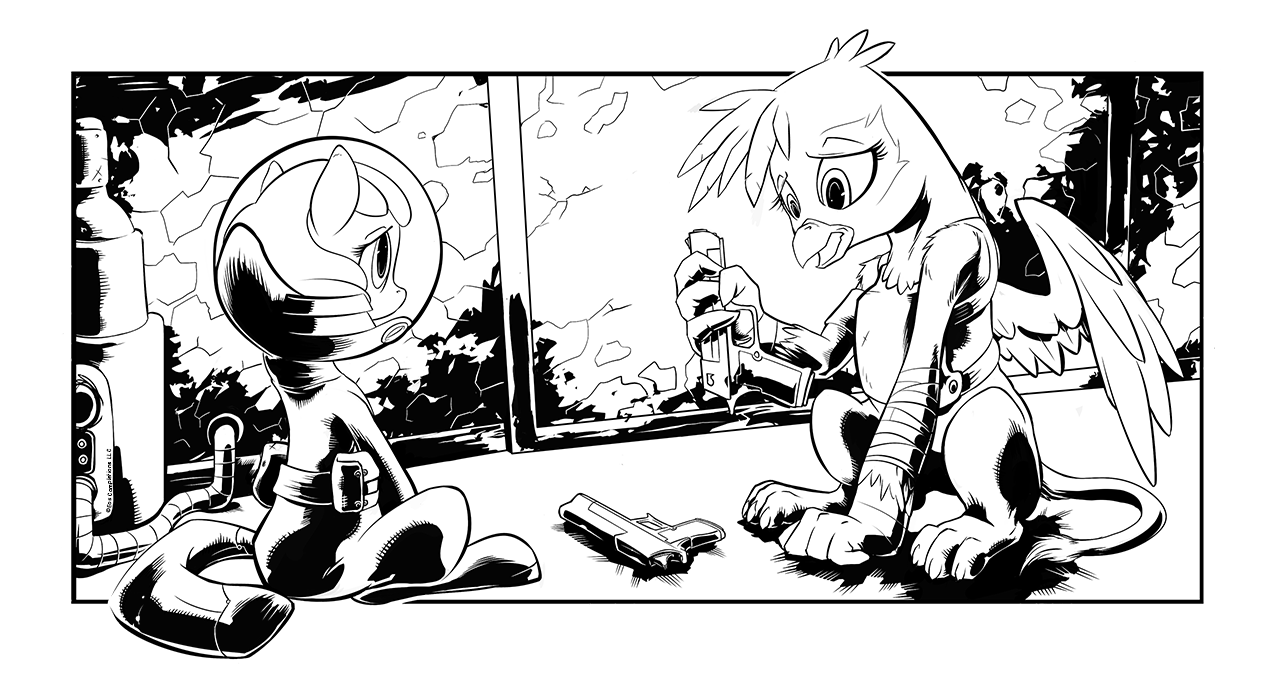
\includegraphics[width=\linewidth]{image06.png}


\begin{intro}
    兰斯洛特,加拉哈德还有我一直等到日落,然后突然杀出去,把那些法兰西鬼子打得措手不及——他们甚至没来得及拿起武器!\footnote{这里是亚瑟王故事的节选}
\end{intro}

{\rt 晚上好,我最亲爱的听众们!你正在收听的是孤狼的52电台!这个频道有你们最想知道的52国道大新闻!}

然后是一阵班卓琴的短暂音乐声。

{\rt 让我们先从正事开始讲起,你们想要知道太阳是什么样子吗?问白苹果们吧!昨晚一个巨大的光球就在盐块城东边十公里左右的距离炸响了!很幸运的是,那里基本都是辐射蜥蜴和遗弃的窝棚。不过那光线就算在隧道镇甚至赤兔领土也能看得一清二楚。如果你觉得这件事非常疯狂,我要和你说,这个可是昨晚百老汇歌舞秀的一部分!首先我们看到一个载满尸鬼的气球升空——就是在盐块城圆顶肆虐的那些尸鬼!陪伴他们升空的是一个叫快乐帕比的小马表演的灯光秀,还真是个奇怪的名字,是吧,不过这个名字似乎听起来很耳熟吧?没错,她就是嘉年华的那位小幼驹!}

然后是一阵胜利的号角声。

{\rt 那么大家问我了,这新闻有什么意义?给那些『懒得听故事直接听结果的观众』一个简单版本!以后在盐块城郊外再也不会受到野生动物和尸鬼的袭击啦!}

然后喇叭里面传来一个拉枪栓的声音和一发枪响,然后还有一个非常硬汉的声音说:「{\rt 后会有期,丫头。}」

{\rt 我爱死这个小家伙了,两个城镇的问题被一个不会脱防辐射服的小幼驹解决了!就算我不是未卜先知,我也知道她一定会往南前进,那么……接下来是什么呢?她要重新开放隧道么?我说,孩子,如果你碰巧路过盐泥沼泽的荒芜之地,你一定要来看你的头号粉丝!我很想知道头盔里面的小脸有多么可爱!好了,现在和往常一样,来点超酷的音乐吧!}

\begin{song}
左一个小马,右一个小马

Here's a pony there's a pony

\medskip

还有一个小小小马,

and another little pony

\medskip

可爱的小马,快乐的小马,

funny pony party pony

\medskip

这就是小小小马!

pony pony sprite\dots
\end{song}

\horizonline

\daytimeplace{5}{16:45 PM}{165战指,盐泥沼泽}{165Th Brigade field Headquarter, Salt Marshes}

% TODO: 检查翻译

「关了那鬼音乐,老娘都听不到那死鬼是不是在外面了!」年轻的狮鹫怒气冲天地瞪了帕比一眼。

「但是……很好听啊!你真是个坏脾气小鸡!」小雌驹皱着眉头又抱她的萍琪派玩偶去了,「别担心丝尾,她没发火,只是累了。」

狮鹫赫瑞塔走到帕比身边,拎着她的头盔把她抓起来,好让她看着自己的双眼。「老娘最后一次警告你!是狮鹫!不是小鸡!外面老大一只蝎尾狮想把我们当晚餐,你丫还一个劲儿地找茬儿,是不是想死啊你?」少女的尖叫声又慢慢低了下去,「我真希望我老爸赶紧回来,」她叹了口气,「或许他能帮我逃出去,然后我就再也不用看你那张傻兮兮的脸了。」

「人家才不傻……你才是个坏心眼猫,我再也不想做你的朋友了!」

「{\mt 警告,检测到敌对狮鹫,距离3米,威胁等级:高。}」

「唉,别说啦,声音先生……」帕比做出一副夸张的厌恶表情转过身去。

「你让谁别说了?你和谁讲话呢?」狮鹫忽然睁大了眼睛。「你那东西还带无线电?」狮鹫跳到帕比背上用力想脱掉她的头盔。「我们可以呼叫支援啊!快叫我爸爸,他在 \SI{90.08}{Hz}!呼号炙红!」

幼驹被吓了一跳,「喂喂,等等!我要先问问声音先生!他住在这个防护服里面,操作那些奇怪的东西。」小雌驹举起蹄子嘘走赫瑞塔,不过狮鹫已经躲一边去了。

「等等,什么声音先生?这防护服能说话?」

「当然可以!这是最好的太空服!而且它超级聪明!」帕比自豪地笑着。

「对哦……」赫瑞塔嗤之以鼻,「比你聪明多了。」

「当然,比我聪……」小雌驹的笑容变成怒容。「喂喂!怎么能这么说人家!」

狮鹫被她逗乐了,「你丫这么简单的招都会中么,你这小鬼太搞笑了,自己承认自己比个香蕉睡衣都蠢!」赫瑞塔说着用爪子弹了一下小雌驹。

「喂喂喂!干什么呢!坏心眼小鸡!如果不是你爹地伤得那么重,我早就教训你了哦!」

赫瑞塔一下愣住了,盯着帕比问:「我老爸怎么了?你怎么认识我老爸?」

帕比看着少女充满希望和惊恐的表情,觉得自己应该非常非常非常谨慎地选择自己下一句话。

「呃……上次我见他的时候,他状态是……死亡,或许他现在已经好点儿了?」幼驹满怀稚气和天真地微笑着。

「我……老爸……死了?你怎么知道的?你什么时候看见他的?这不……这不可能!他是最棒的!不可能死的!你绝对看错了!快跟我说这不是真的!」狮鹫拔出她的白色手枪,带着黄色条纹的枪口指着幼驹的鼻尖。「快说!你看错了!」

赫瑞塔发红的眼睛死盯着帕比粉红的眸子——幼驹虽然有点结巴,但是那双闪闪发光的粉色双眸绝对不可能撒谎,她只是一个稚气未脱的小孩子。

「我……我不知道,他……只是跟我说……他想和你说,他非常非常非常想和你在一起,他很抱歉,所以我超级快地跑过来找你,因为我觉得他看起来伤得很重,而且我很想我妈妈……」

「住口!」赫瑞塔一爪子把帕比拍飞到了墙上,跪在地上把头深深埋在双臂之间,不敢面对残酷的现实。「这不是……这不是真的……我爸爸……是最厉害的赏金猎人……他绝对没事的,他一定会赶来救我……我……我……」

一个金属碰撞的铿锵声让少女抬起了头。

帕比站在赫瑞塔面前,幼驹什么也没说,只是把那柄带着红色条纹的黑色手枪放在狮鹫面前,然后又蜷缩回房间的角落。

「黑玫瑰……」年轻的飞行员吃惊地瞪大眼睛看着面前的枪。「不……不……不会……不可能的……这不是……」她又一次看着穿黄衣的小马。「拜托……求你告诉我……这不是真的!我只是在做噩梦!」

帕比皱着眉头低下了头,「我……我不知道……如果这是一个噩梦的话,那我醒来的时候,妈咪一定会在我身边安慰着我,所以……我希望这也只是一个长长的噩梦……」幼驹又叹了口气,「但是,我不觉得这是……」

「肏!」赫瑞塔用爪子抓起那个手枪,和她自己的点45手枪完全一模一样,除了颜色。「到底发生了什么?为什么你会在现场?」\emph{冷静点儿,赫瑞塔,别情绪化了,你应该问清楚她情况,你可以做得更好,你必须做得更好!}

% NOTE: . -> 点

「我看到天上好像有四个小鸡……」

「不!准!叫!老!娘!小!鸡!我们是狮鹫!比你们这些蠢小马厉害几百倍!你要再叫老娘一次小鸡,那就是你丫这辈子的最后一句话了!懂不懂?」狮鹫拎着帕比的脖子,另一只爪子举着枪顶着她大吼道。

幼驹的眼睛充满了恐惧,她挣扎了两下想要逃跑,但是很快就放弃了,她大哭起来。「我……我很抱歉狮鹫小姐!我会乖乖的!别……别欺负我……」

赫瑞塔点点头把她放下来,「这下好多了,有四个狮鹫在天上飞,然后呢?」刚才的怒气似乎冲散了狮鹫的其它情绪,让她可以更认真地听帕比讲下去。

快乐帕比结结巴巴地继续她的故事,不想让可怕的狮鹫再发火。「就是刚刚,我和朋友正顺着路走,然后天上……呃……天上……开始好像是他们在跳舞一样但是他们看起来好多受伤掉了下来我走过去看他们最后掉下来的一个跟我说给你那个黑东西然后和你说他很抱歉他想往南去我戳戳他想让他醒来但是他还是一直睡我真的真的真的很努力去戳他让他醒来但是他就是不醒来!请别对我发火我真的真的真的想让他好起来但是声音先生和我说他已经『死亡了』而且……而且……」幼驹后退了几步,缩成一团,用前蹄抱着头盔。「请不要欺负我,我真的没有恶意,我只想帮忙!对不起!」

\emph{肏,算了,她只是个孩子!}狮鹫摇了摇头,自己的怒火也开始消退,这个幼驹估计都不知道『小鸡』对狮鹫而言是侮辱性的称呼……趁她还没给自己惹上真正的麻烦之前,某狮鹫还是好好教她吧。

「那个某狮鹫还能是谁?」赫瑞塔长叹一口气,轻轻拍着帕比的头盔,「好了没事了,真的,叫我赫瑞塔,或者赫瑞好么?你只是有点……没教养,别担心,我教你就是。现在我们还是想个办法出去吧。」

「但是……你刚刚还对我发火……」帕比还是双蹄抱头的蹲防姿势。

「我没生气,真的……做个好孩子,站起来,好不好?」

「但是我叫你小鸡还说你是坏蛋……」幼驹小心地露出脸。

「别那么叫了行不行?我也对你吼过了,我们扯平了,可以吧?」

「所以……所以我们还能做朋友?」帕比满怀希望地问。

狮鹫叹了口气,「对,我们还是朋友……现在让我安静一会儿,我好想个办法出来。」

对,办法,说起来简单做起来……好吧,不是一般的难,但是至少这些话还是让帕比再次变回了快乐模式。幼驹点了点头坐在楼梯上,狮鹫看着外面,那猎食者估计在哪里躲着,等她们自己走到空旷地去。

「没戏……要是我有比枪更厉害点的东西,或许还能拼一下,不过如果……」狮鹫回头看着帕比,「我说,你不会刚好带着爆炸物或者重武器吧?」

「我有一个石头!超耐磨!」帕比自豪地把「命运之石」展示给赫瑞塔看。

狮鹫不屑地嗤之以鼻,「还真是CNM!抱歉,我可不想把我的命赌在这块蠢石头上。」

雌驹歪着她的头,一脸不解地看着她最喜欢的武器。「小石石,我才不觉得你蠢……不过现在你还是回包包里睡觉吧。」

「拜托!老娘正在想个正儿八经的主意呢!别在这儿和你包包里面的东西挨个吻别了,你他喵的能做点有用的么……比如……比如说……算了,你还是去和你的闪尾玩去吧。」

「丝尾!」

「对,就是那玩意……一边玩去……」

「好的好滴好的!茶点五分钟就来!」帕比坐在楼梯上开始和她的萍琪派娃娃聊天。

「无论如何……」狮鹫开始低声自言自语,「附近没有任何掩体,我估计只能带着那东西跑个几分钟,好吧,我们真的需要重火力……」赫瑞塔无奈的叹着气,「简直太扯了,外面的坦克装满各种炮弹,我们蹲在这里,只有三把点45手枪和一个……石头……」

% NOTE: . -> 点

这个时候,帕比正在把她的玩偶放在一枚大号坦克炮弹弹头上,然后用另一个当做茶壶来沏茶。「喏,你杯子里面要6块还是8块方糖?呃……你有杯子么?」

「不,谢了,我不要,我想我有个办法了。」狮鹫完全懒得去看幼驹在做什么,她一边继续观察着外面一边说:「我先跑出去吸引那蝎尾狮的注意,等他开始追我的时候,你冲到最近的坦克里面,你最好快点,因为我不能带他跑太久,你要找的是高爆弹头,那东西又大又亮,像一个尖头大水壶,而且上面有个红条,懂了么?」

「呃……好吧……」帕比看了看她蹄子上的『水壶』然后耸了耸肩把那东西放一边,「那你能帮我看好丝尾么?」

「我觉得我们出去之后你的玩偶也不会跑哪儿去的,你丫就给老娘利索点儿,去坦克里面拿个有红头的大『茶壶』回来,等你搞定这事儿之后我们再继续下一步计划。」狮鹫蹲下来,活动一下筋骨准备冲出去,她现在需要自己是最佳状态。

「但是……她会害怕!」幼驹继续冒着傻气。

「帕比,闪尾只是个玩偶!她不可能害怕!」赫瑞塔扭头抓起那个萍琪派玩偶,在幼驹面前晃着说:「看到没?她在笑!她没关系的!回来时候说不定她还能给我们办个……高爆弹?」狮鹫瞪大眼睛看着帕比玩具的那个椅子。「呃……你从哪儿找到这个的?」

黄衣幼驹开心地说:「炫彩大厅!软气给我的!」

「不是……我是说这个椅子……」

「哦,这个啊……在那个坏掉的大铁马车里面,闪闪发光哦,我拿了好几个。」看着狮鹫的表情,帕比于是又说:「你想要吗?」

赫瑞塔眼角抽搐着,「这……真好……第一步完成了……现在我们开始第二步……」

「但是我们什么都……」

「好了,啥都别说……我们,第二步,懂了吗?」狮鹫觉得自己的自控能力越来越好了。「你仔细听好,我把那个大坏蛋引到这个塔的门口,当那蝎尾狮探头进来的时候,你就把这个弹头丢进他嘴里,然后我就打爆他,然后乒,炸飞他的头,然后坏蛋就死翘翘了!」

帕比皱了皱眉头,「就是说……我把茶壶丢进他嘴里然后电影就结束了?」

「电影啥?哦对,把那东西丢进蝎尾狮嘴里,然后我处理剩下的事,好了,你准备好,别吓坏了,懂?」

「好的好的……」幼驹抱起弹头然后躲在墙后面,赫瑞塔谨慎地展开翅膀探出头。

不过一分钟,外面就传来枪声,还有一大堆帕比完全没有听过的精彩狮鹫方言骂街,幼驹超超超好奇外面到底发生了什么,但是赫瑞塔叫她乖乖呆好。现在幼驹觉得有点麻烦了——如果赫瑞塔发现她溜出去了那么一定会很生气,她生气起来可害怕了……但是帕比觉得外面一定有什么超级酷的事情发生,而且生怕错过了。

「或许稍微稍微稍微看一下下……」听着外面的怒吼声和枪声,幼驹抱着她的高爆弹,小心地爬到了门口。「就看一下下……一下下……绝对没关系的。」

「哎,啥都看不见!这不公平……」

忽然一个残影飞快地冲过门口跑到房间的对面大叫着。「就是现在!」

「现在啥?」帕比有点奇怪地问。

嗷呜!!!

随着一阵水泥碎块飞溅,蝎尾狮脑袋冲进门来,但是身体却卡在门框上进不来,帕比发现自己就距离那巨兽的尖牙只有几厘米的距离,让她吓得尖叫一声坐了一个屁股蹲。

「你丫搞什么呢!快丢那劳什子然后趴下!」赫瑞塔惊恐的大叫起来,「给老娘动起来!」

黄色幼驹大叫一声发射了炮弹——那弹头画了一个小小的抛物线,而帕比则以一个更大的抛物线向后蹦了出去,在弹头落在野兽面前的时候,狮鹫举起了枪。

乒!乒!乒!

% NOTE: 呯 -> 乒

三发射击,三发命中,三发跳弹。

「肏!谁尼玛把弹壳做这么厚枪都打不穿!」

双枪少女一边骂着一边把手枪里面的所有子弹都倾泻在那个破弹头上,但是却什么都没发生。

「肏,肏,肏,没用!」赫瑞塔收起双枪然后拿出第三把手枪,那把黑色并且有着红色条纹的手枪——这把枪和她的另外两把没什么区别,她把一梭子子弹打在蝎尾狮鼻子上,终于让那个怪物退缩了一下。

「我想他正在把入口弄大。」帕比又后退了几步,而且看起来没那么害怕了,幼驹轻轻敲着自己头盔下巴的位置,看起来好像在分析战局。「他好厉害哦!」

野兽血红的双眼瞪着赫瑞塔,显然他不打算再回外面蹲伏去了——即使这意味着他要把整个指挥塔拆掉来抓狮鹫,而且他也正在拆了,虽然拆得有点慢。

「在那傻站着干啥,赶紧滚过来!」狮鹫一边给手枪装子弹一边吼着。「就算老娘手枪打不响,但是如果打中引信还是能把你的屁股炸开花,你丫给我找个掩体蹲好!」

「吟新……是啥?」

赫瑞塔忽略帕比的又一个傻问题,从掩体跳出来,双枪瞄准那个炮弹的引信,「说拜拜吧,你这个……」

就在这时,年轻的飞行家注意到蝎尾狮正在低着头弓着身子做出飞扑准备动作,等赫瑞塔飞到空中的时候才知道蝎尾狮的弹跳能力有多好,但是已经太迟了——她连骂街的机会都没有,一瞬间就被蝎尾狮的爪子像拍苍蝇一般从天上拍了下来。

赫瑞塔被蝎尾狮有力的爪子按住了肩膀,她无助地挣扎着,被蝎尾狮撕扯着。

快乐帕比也同样惊恐地尖叫起来,幼驹想后退,但是自己的臀部已经碰到了墙壁,蝎尾狮非常非常可怕,它正在伤害赫瑞!

那一瞬间,帕比看到的不是蝎尾狮,而是一张双眼闪着光的粉红色金属面具。

「\emph{求你……哈哈哈……别让我……哈哈哈……笑了……\footnote{嘉年华的瑞吉}}」

帕比双眸之中点燃了粉色的火焰,她举起蹄子大喊:「石头!」

「命运之石」立刻飞到她的蹄子上,幼驹高高跃起冲向那个野兽。

「放开她!快放开她!」

蝎尾狮被黄色的小小奇袭打乱了节奏,他把自己的旧猎物丢到了一边,怒吼着转向小小幼驹。然后张开血盆大口,随着清脆的咔嚓一声,黄色的小雌驹消失在怪物嘴中。

赫瑞塔尽力保持自己的清醒,挣扎着爬上楼梯,而那头蝎尾狮得意地吼叫声为帕比的命运盖棺定论。

「不……不,已经太迟了……快逃命吧……别回头看……」重伤的狮鹫一边自言自语,一边爬上楼梯,只是走这几步身上的伤口就让她痛得快昏过去了,身后蝎尾狮正在疯狂地怒吼着,估计正在撕扯那可怜小家伙的尸体,赫瑞塔拿出一瓶治疗药水一饮而尽,然后转头看着楼梯下面。但是她只能看到一片粉红色的烟雾,接下来伤口的剧痛和失血让她失去了意识。

……

现在,还是让我们为那个非常不走运的蝎尾狮默哀一分钟吧。

这就是为什么说『绝对不要随便乱吃东西』,因为那肉显然已经变质了。

\horizonline

\daytimeplace{6}{00:45 AM}{165战指,盐泥沼泽}{165Th Brigade field Headquarter, Salt Marshes}

「{\mt 系统重启完毕,所有功能恢复,自检系统上线,目标001:快乐帕比,雌性陆马,目标已死亡,体征状况稳定,完毕!}」

懒洋洋地睁开眼睛,帕比打了个哈欠。「外面还黑洞洞的呢……」睡觉的时候还被什么重物压着,这让她很不开心。

「发生什么事情了?小鸡呢?大坏猫呢?」

「{\mt 分析中,监测到敌对生物,距离6米,赫瑞塔,威胁等级:可忽略。}」

一个红点在罗盘上闪烁着。

「傻声音,赫瑞不是敌对圣姑!」

那个红点变成了粉色。

「很好,我们出……咦?」蹬着蹄子却发现自己没在移动,帕比这才注意到她挂在灰白色的杆子上。花了吃奶的力气,帕比好不容易从蝎尾狮的骨头堆里面钻了出来,那个野兽的骨架看起来已经和墙壁的颜色一样,似乎已经和墙壁融为一体,而那个长满利齿的白色骷髅头仿佛正在绝望地嚎叫,翅膀的骨头也伸开,似乎它不顾一切想要逃开那吞噬它的致命粉云。

帕比走到了赫瑞塔身边,但是狮鹫却一动不动地躺在地上。

「声音先生……她是不是……你知道的那个……死了?」

「{\mt 分析中,否定,目标失去意识。}」

「哦……这表示她会好起来?」

「{\mt 肯定,目标恢复中。}」

「好滴!」这句话对于帕比来说就够了,她开心地隔着头盔和赫瑞塔吻别。

「我很抱歉,但是我必须走了,小鸡,我妈妈还在粉箭头的末端呢!」

帕比走了几步,但是又退了回来。她觉得只是吻别似乎不够,幼驹拿出萍琪派玩偶然后放在狮鹫的爪子中。

「听好,丝尾,帮我照顾赫瑞塔,别让坏事发生在她身上。」

这次没什么问题了,帕比开心地跑到外面,然后捡起自己的滑板车。

「嘿,能来点音乐吗?」

\begin{song}
在丛林中,密密的丛林中。

In the jungle, the mighty jungle,

\medskip

今晚狮子在沉睡。

the lion sleeps tonight!

\medskip

在丛林中,恬静的丛林中。

In the jungle, the quiet jungle,

\medskip

今晚狮子在沉睡。

the lion sleeps tonight\dots
\end{song}

\horizonline

\daytimeplace{6}{10:00 AM}{狮鹫陨落之地,盐泥沼泽}{Griffon's Fall, Salt Marshes}

不用铲子挖坑本身就是一种折磨,而在泥泞之中,用你自己的爪子挖自己父亲的墓穴,简直就是……

大颗的泪水顺着狮鹫的喙滑落,每一次她想要挖出泥土,就会有更多的泥水落回来。但是她却无言地继续挖着,他从来没让她哭过,他是最厉害的最顶尖的佣兵,但是现在他死了,被鹰爪佣兵\footnote{鹰爪佣兵 (Talons):狮鹫公国被英克雷吞并之后,流亡的狮鹫组成的大型佣兵组织,大多数狮鹫都属于鹰爪佣兵}杀害了。

赫瑞塔把他拖进浅浅的墓穴里面,尸体在泥泞之中发出湿软的声音,女儿看着自己父亲的鲜血渐渐渗入泥土之中,努力把自己的泪水咽下去。

他喵的……这个墓穴甚至不能装下他。

「这不公平,把我自己孤零零地丢在这里……我现在还能去哪儿?」赫瑞塔叹息着,她想要发火,但是却一点怒气都没有。他已经走了……还能怎样。

「为什么……」

肏!

肏蛋!

狮鹫慢慢地用泥土和附近的碎石将墓穴盖好。她拿出黑色的手枪,迟疑了一下又放了回去,然后拔下自己的三根羽毛,然后放在她父亲永远安眠的胸口附近。

「跟老妈说我会照顾好自己的,明白吗?」

赫瑞塔揉了揉眼睛,然后拿起她的包,看着包里面漏出来的丝尾,凝望着那玩偶的蓝色双眸,她再一次露出了笑容。

「我会照顾好自己的。」

\horizonline

\daytimeplace{6}{11:30 AM}{随机遭遇地点,盐泥沼泽}{Random encounter location, Salt Marshes}

「嗨!我叫快乐帕比!」

三个奴隶贩子当中的黑色陆马皱了皱眉头,「我想我听过这个名字……或许我们还是别……」他看了看另外俩伙伴——他们都和他一样武装到牙齿。但是前两天他们都听过孤狼说到的游荡在52号国道北边的幽灵。

「我才不怕幽灵,血滴,如果一个幼驹就能把你吓出翔来,那你就滚边一去!」看起来是奴隶贩子头头的黄色独角兽打量了一下他自己的『货物』,两只公马和一只年轻雌驹……完全不如往常的多,「四十钉,抓住她!」

快乐帕比有点迷糊,在罗盘上有六个点,三个是粉色,另外三个是红色……声音先生总是搞奇怪的东西出来,一个红点的小马靠近她,然后小心地把蹄子放在她背后。

「小子,跟我们走,别反抗!」

「好的,好得!我们去哪?」黄色的幼驹一脸兴奋。

对于新奴隶而言,她的举动很明显非常奇怪。她身边那只小马,绿色的独角兽看了看他老大,而后者耸了耸肩,「看到了么,这就是被卖了还帮着数钱的典型,给她带个项圈。」

四十钉想要剥开帕比的外衣,但是他显然不是和平部的技师。

「我说,老大,这破玩意弄不开!」

「呃……我也脱不下来,这个头盔粘得厉害……我还试过打碎它,但是它不停地自动修复!」终于有小马帮帕比解决太空服问题了,不过他们看起来完全没有足够的知识和技巧。「我想或许会有个开关啥的,但是每个开关都没用!」

「闭嘴,白痴!」四十钉显然没有耐心了,所以他还是用最原始的办法解决问题。他举起一把超大号扳手然后砸在帕比的头盔上,把头盔表面砸出蜘蛛网一样的裂痕。

黄色独角兽咆哮起来,「你丫要敢砸碎她脑袋,老子就把你的脑袋也捎带上!死幼驹一文不值!」而那个黑色的奴隶贩子看着另外三个奴隶,对这一幕喜剧窃笑着。

帕比害怕地后退一步。

「我说,这太危险了吧!」

「{\mt 警告,罗盘失灵。警告,感应器离线。警告,头盔受到破坏,修复中。}」

「卧槽他喵的,这蛋壳还真结实!」绿色独角兽再一次举起扳手的时候,看到那个裂痕已经完全消失了。「我勒个去!」

「用个绳子给她捆起来然后赶紧走,等我们从这个屎坑出去之后再处理那问题。」

他们叫帕比乖乖地,于是帕比就乖乖地看着漂漂小马给她脖子上套了一个绳圈,他们把她和其他奴隶一起拽着走的时候,帕比觉得有点不对劲。

「喂喂,我不能把我的车子丢那里啊!」幼驹走向她的滑板车,但是那个奴隶贩子把她扯了回来。

「你丫想去哪?」

帕比挣扎着说:「我的滑板车!放开我!」

四十钉冷笑了一声,「没错,小婊子,」他把小雌驹扯到面前,看着她的眼睛说。「你现在是奴隶了,把你的滑板车和别的什么东西都忘掉,如果你还想活命就给我乖乖地,听明白了么?」

「但是……我要去那边!」帕比用蹄子指着南边。

绿色的独角兽啐了一口然后用他的枪柄打着幼驹的屁股说:「给老子闭嘴,竖起耳朵听好,要不然肏爆你这个小婊子的屁股!反正不听话的小马卖不了好价钱!」四十钉转头对奴隶主说:「喂,老大,我要给这小婊子上一堂礼仪课!」

「别把她玩坏了,不然你要掏她的钱。」领头的头都懒得回,继续往前走。

黄色的幼驹皱着眉头。「先生你不可以说脏话……」她的表情看起来好像绿色奴隶贩子刚刚打她的那一下完全不疼不痒。

「闭嘴!」

帕比被打得飞了出去,摔出几米远,「喂喂,别这样粗鲁,会有马受伤的!」她一脸完全没事的样子站起来,反而有些担心地看着四十钉。

「怎……怎么回事……你是啥玩意?滚远点,别动!」奴隶贩子举起枪瞄准幼驹。

乒!乒!

% NOTE: 呯 -> 乒

两发子弹在幼驹胸口打出两个洞,但是她完全没有反应,四十钉惊恐地瞪大眼睛,这个时候奴隶主回头怒视着他的走狗。

「肏你娘的龟孙子!你丫吃错药了么?这是你最后一次杀我的奴隶!」黄色独角兽低头冲向绿色小马,把他撞飞到一边。

「不……我……我才不要死在这里!」四十钉一脸惊恐转头把弹夹里面的剩下子弹射向他的老大,那个奴隶贩子头头还没反应过来发生了什么膝盖就被打碎了。跪在地上的独角兽拿出他的突击步枪开始乱扫起来,黑色的陆马也拿出一把散弹枪,乱飞的子弹又在帕比身上打了一个洞,但是看起来完全没有影响到幼驹。

「别吵架啊,喂喂!我说!你也是!」帕比想要恢复一些秩序,但是显然事态已经超出她的蹄下。

「你们都是大坏蛋,你们不觉得害臊么?声音先生,做点什么啊!」

「{\mt 修理完成,气密性恢复,目标001:快乐帕比,已经死亡,体征正常,完毕!}」

「不是这个『什么』,是做点别的『什么』!」

黑色的奴隶贩子掏出一瓶治疗药水刚想要喝下去,他的枪就被另一个公马奴隶夺了过去,然后那张丑脸就被一发散弹打得四分五裂。俩受伤的独角兽倒在血泊之中对射的时候,那个怀孕的雌驹正拼命地想在这个尸体背后寻找掩蔽。

四十钉比起他流了一大滩血的奴隶主还多了一口气,不过他不想独自下地狱,随着他的角发出光芒,所有奴隶项圈上炸弹的遥控器从他背包里面飘了出来。他躺在地上一边咳血一边露出狰狞的笑容,「别害怕……咳咳……小马们……咳咳……你们……会先……咳咳……死!」他举起他完好的蹄子慢慢伸向开关,两个还活着的奴隶惊恐万状地看着他。

「没收!」一个黄色的蹄子从他面前把引爆器夺走了,「坏小马不能玩玩具!」帕比用她最认真的表情看着他。「我说了别发疯!在你乖乖坐好之前这个由我保管!」小雌驹一脸严肃地说:「我说到做到!」

奴隶贩子看了看帕比,然后仰天长叹,「我……真难以置信……我……咳咳……一直听……咳咳……幽灵的故事,」他的眼睛看着帕比防护服上的最后一道划痕消失,「你丫……咳咳……比我想得……咳咳……还要可怕……一万……」他的声音和生命一起被饥渴的废土吞噬了。

\horizonline

\daytimeplace{6}{8:30 PM}{隧道镇外,52号国道北口}{Tunnel Town Outskirts, Big 52 N Branch}

「当小马妈妈和小马爸爸超喜欢对方的时候,他们就写信给塞拉斯蒂娅公主要一个小幼驹,你们真的不知道吗?」帕比一边在附近蹦来蹦去一边说。

在盐泥沼泽冗长但是又幸运的散步之后,那无穷无尽的泥坑终于抛在他们身后,路面变成了崎岖的山路,随着夜幕降临,远处的景色渐渐模糊,夜间的掠食者也出来活动,帕比的HUD上闪烁着野生动物的红点,但是它们基本是被她的超自然力量惊得四处逃窜。

那对和快乐帕比一起走的小马也一样苦不堪言,那个叫甜花的奶白色怀孕雌驹先开口了:「差不多……呃……大概就是这样……你真的挺能说的。」

「没错!大家都这么说!」帕比微笑着继续说:「我希望你能有一个小雌驹,小雌驹超可爱!」然后她压低声音说:「而且,我听说男孩子身上都长虱子,不骗你!」

甜花咯咯笑着,轻轻蹭着她的伙伴,那个叫阿索的棕色陆马。「她这一点没错,是吧?」

阿索笑了笑:「那景色看起来非常壮丽吧!」公马停了下来看着远方。「我们到了,小家伙,这就是大隧道。」阿索用蹄子指着山崖边上的灯光说。

一座用石头搭成的巨大拱桥穿过泥潭,直接爬上山崖,就像是通向天空的大道一样。帕比瞪大双眼看着这壮丽的大桥,就像是大陆直接射向山崖,然后,乒——炸成了一堆五颜六色的灯光。不过她的两个伙伴似乎对她更感兴趣,因为幼驹双眸射出的粉色的光芒穿直切切穿过黑暗,而在她头盔上也漂浮着一圈淡淡的鬼火。

「好滴!那么,我们现在就去那边么!妈妈在那里等我呢!」帕比兴奋地问着,完全没注意到那两个小马在相互使眼色。

「呃……不过……我们不住在那里……而且你进隧道镇还要交税,我们去荒芜之地的贸易站,那里稍微远一点。」阿索有些迟疑,但是雌驹蹭了蹭他,鼓励他说出他们的想法,在顿了顿之后,公马低下头继续说。「我……我们想知道:你真的是个幽灵?还是上天派下来保护孩子的守护天使?」

帕比歪着头,然后咯咯笑起来,「我是快乐帕比,漂漂笨马!我不知道为啥大家都叫我幽灵,我只是在找我妈妈!」

「对……你和我们说了上千次了……」阿索耸了耸肩看着他的伴侣,「那么,我想就这样了……毕竟我们欠你……那么……可以接受我们只是说『谢谢』么?我真的很想用什么东西报答你,但是我们在活着回家之前真的什么都没有。」

「好的好滴好得!拜拜漂漂马!」帕比注视着她的新朋友消失在夜色中,然后顺着桥走向隧道镇。

~\vfill

\begin{note}
    升级 (Lv 5)

    新技能解锁:快速训练:力量($5 \to 6$)你现在能在包包里面塞好多好东西了!
\end{note}




\chapter{临时保姆}

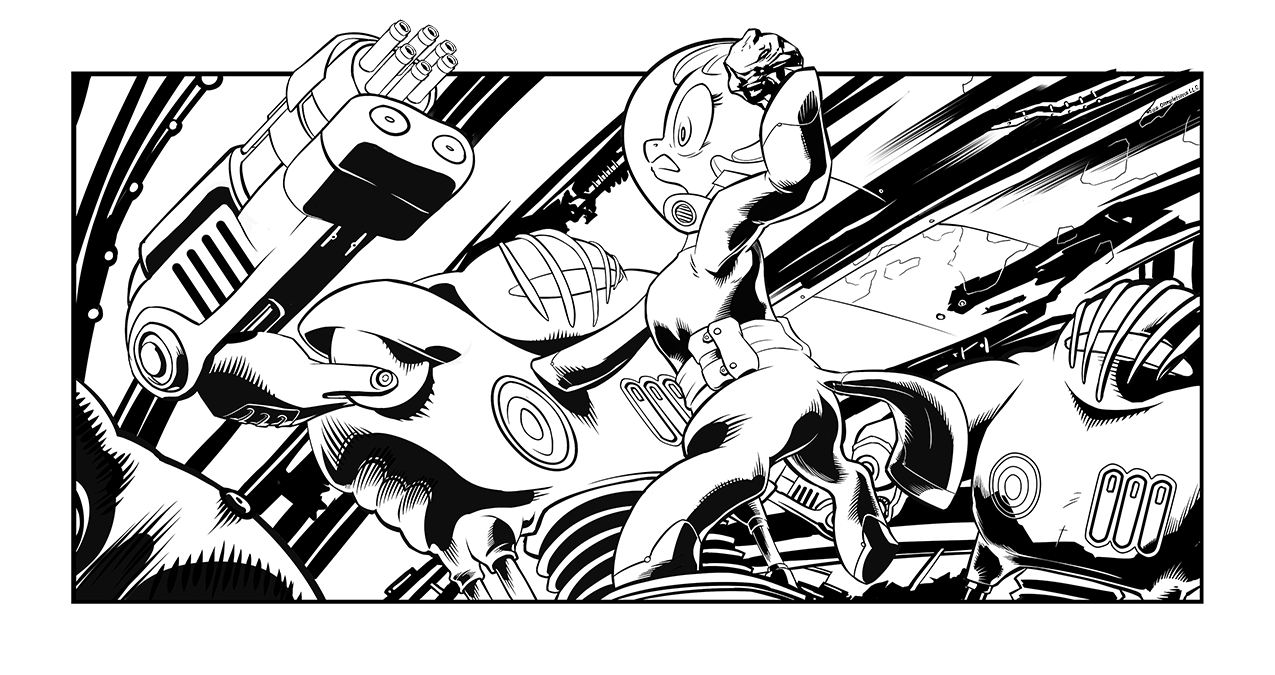
\includegraphics[width=\linewidth]{image07.png}


\begin{intro}
    什么?你说那些可爱的小天使?照顾他们完全没有问题!
\end{intro}

\daytimeplace{6}{9:00 PM}{隧道镇,52号国道北口}{Tunnel Town, Big 52 N Branch}

快乐扳机 (Trigger Happy) 已经当了半辈子卫兵,她很确定自己见过各种各样想要进隧道镇大门的家伙。不过她现在觉得自己见识还是不够。现在她所有的卫兵同僚都战战兢兢地缩在她背后——只是因为那只穿着滑稽的幼驹现在看起来更不开心了。

「唉,你们这些胆小鬼,算了交给我来吧,你们放松点儿。还有看在我尾鬃的份儿上,别乱开枪。」

独角兽雌驹走出那群卫兵,朝那只被粉色鬼火环绕的黄色小幼驹走去。

「你,就站那儿!别再靠近了,告诉我你到底是谁?」

扳机并没有期待那只幼驹乖乖听话,不过看着她坐下,守卫队长还是松了一口气。

奇怪的孩子挥着一只蹄子向她打招呼:「嗨!我叫快乐帕比!你看到我妈妈了吗?」

扳机皱了皱眉头,「快乐帕比……你就是那个小幽灵帕比?」

「我不是幽灵,我只是个小雌驹!」幼驹嘟起了嘴,她背后还背着一个长长的红色滑板车,看起来不像是武器,虽然的确很大。

「你想说,你就靠一个红板\footnote{红板 (Red Racer):飞板璐长大之后开办的玩具公司销售的主打产品,速度非常快的滑板车,虽然对小孩子略有些危险,后来小璐靠卖这个赚的钱和其他CMC一起成立了避难厩科技。}一路从盐块城穿过盐泥沼泽跑到这里?」

帕比咯咯笑起来,「才不是,胖胖独角兽走得超级慢,所以我也得慢慢走。」

「谁谁谁?算了,别提这个了。」扳机叹息着,「我要过去了,你别做……呃……那些鬼鬼怪怪的事情。」

她回头看了一眼,正好和掩体后面露出的三对惊恐的眼睛对上,其中之一还举着一面小白旗晃了晃。她真心向女神祷告,祈求能有几个更靠谱的队友。然后她走向帕比。

「嗨!你好漂亮!漂漂小马姐姐!你叫什么名字?」幼驹露出她最友善的笑容。

\emph{她只是……只是……只是一个有对发光双眸的幼驹而已,估计只是受了点辐射影响。}「没搞错吧,你就是新闻说的那个快乐帕比?那个来自盐块城和嘉年华的幽灵?」卫兵笑了起来,「拜托,别扯了!」

帕比也跟着笑了起来,「哈哈哈!很有趣对吧!呃……不过哪里有趣了?」

幼驹的问题让卫兵队长笑得更响了,「快乐扳机,但你叫我扳机就好。」

帕比皱了皱眉头,「啊,我能叫您乐乐么?」

「当然,对了,我还有个东西……」扳机拿出一片黄色的塑料卡递给帕比,「这是你的通行证,中午有个叫赫瑞塔的狮鹫来到这里,她一直等你到傍晚,但是你还没来,所以她先走了,不过她走的时候还帮你交了通行费,她说你最迟明天就会来。」

「呃,赫瑞在这里?她还好么?」

「我想……她很好,不过她不太爱说话,不过我也没碰到过爱说话的狮鹫。」扳机扭头往回走。「进来吧,在外面可不利于健康,附近可有不少血翼\footnote{血翼 (Bloodwing):吸血果蝠受辐射影响以后,真的吸血了}。」

「血翼是什么啊?」帕比跟在扳机背后问。

「如果你问我的话,他们就是麻烦!是长翅膀的大号水蛭!」雌驹笑着伸蹄子招呼帕比走进去。里面是一间用沙包和生锈的铁板围成的简易窝棚,两挺加特林机枪在窗口前指着桥头,而墙角堆着一大堆弹药箱——还有三只全身紧绷的小马一脸尴尬地打着招呼。

「伙计们,别这样。这是快乐帕比,嘉年华的小英雄,她和我们可是一伙儿的,所以别害怕好吗?」卫队长举起蹄子掩嘴窃笑,「我还真想看看孤狼亲眼看到他所说的『英雄』是什么样子会有什么反应。哦,这几位是绿梨,坏枪和小豆子。」

「嗨!我叫快乐帕比!」幼驹蹦跶到仨小马面前。看着她的新朋友们一脸紧张的表情,于是她又接着说:「我正在找我妈妈!她或许会在山里面!」

三个守卫之一低声嘟囔着:「这下麻烦可大了……」

\horizonline

\daytimeplace{6}{9:45 PM}{隧道镇,52号国道北口}{Tunnel Town, Big 52 N Branch}

「哇塞!好大哦!」帕比看着隧道入口,一直仰头到一屁股坐在了地上。这个隧道大到可以同时让天空马车和普通马车一起出入,而且有两排车道!隧道的混凝土墙壁在深入山脉20米之后,被一道生锈的巨大铁门硬生生地截断了,那面铁门上是一个白色的天角兽标志,看起来那标志简直比女神更雄壮威武。标志下面是一行字:旭日公司——走可持续发展道路,而字下面,又是一个平常门上都会有的大大危险警告标志。

「看到了吧。」扳机敲了敲那个金属大门,「它封死了,我很抱歉,小家伙,但是这估计就是你旅程的终点了。」

「但是……妈咪在里面!你看那个箭头!它指着大门呢!我得进山里面去!请打开它,拜托!」帕比闪着水汪汪的大眼睛。「超超拜托,漂漂的乐乐姐姐!」

卫兵队长后退了一步,「哎呦,这眼睛绝对该列为违禁武器……不过,我很抱歉帕比,就连我们自己也没办法进去。为了打开它,我们都不知道试了多少次了,不信你看吧,我们现在还是零分。」

「但是我真的,真的,真的真的真的要进去!妈妈在里面等我!」小雌驹满地打滚。

坏枪摩挲着自己的胡茬子,低声地自言自语:「我想那个TNT曾经说过可以从通风管进去?」

扳机瞪了他一眼,「闭嘴!」然后转头满脸堆笑的看着帕比。

「懂了么,没办法进去!」她想板起脸,但是小雌驹早已经不吃那套。

「呃,洞风道?那是啥?拜托,告诉我!我为你做什么都行!哦哦哦,我拿这个跟你换!」帕比忽然掏出一个从军事基地拿出来的坦克炮弹头,这一个上面是黑带,「你看,这个闪闪发光的东西超级厉害!您让我进去我就给你这个!成交么?」

「帕比……这危险了!我不想让幼驹去送死,抱歉。」

幼驹后退一步,看起来她就快要哭出来了。「我才不怕!这不公平!如果你们妈妈被关在里面你们肯定早就打开这破门了!而且……而且……」小雌驹尥蹶子踢着门。「我不能在这里放弃,她在里面!她一定在里面!」

坏枪趴在扳机身边耳语着:「为什么不让她进去,她已经救了俩城市了……我可不觉得她只是个一般孩子。」

独角兽卫兵叹了口气回答:「我们现在根本不知道隧道里面有什么,你好好想想大门关上的那天,我可以清楚地听见困在里面的小马敲门呼救的声音,还有枪声和惊恐的尖叫。」扳机用蹄子敲着坏枪的前额,「你好好看她,就算她也许是个不一般的小家伙,不过她也只是个孩子!我绝对不会送个孩子去踩雷区!」

公马卫兵注视着他上司的眼睛,「你觉得她会就这么放弃?如果她真的是那个幽灵,那我觉得我们也没什么办法阻止她。」

快乐扳机以蹄扶额摇着头,「你还真信那些床边故事?拜托,醒醒吧,她就只是个穿着全套防辐射服还稍微受了点儿辐射影响的小孩子而已!」

这个时候帕比依然站在大门前垂头丧气,「我不是小孩子,我长大了……我还能放飞气球!」她愤愤地朝扳机皱着眉头。帕比脑袋里忽然冒出一个新点子,小雌驹抬起了头,「喂,声音先生,他们说的那通风洞是啥?」

「{\mt 通风道:排风系统,用于将新鲜空气吹入密闭空间的设备,大型隧道使用的通风道通常可以允许小马爬进去以便进行维修——知识小点滴!}」

「哦,酱紫啊……怎么进去,维……维什么那个东西?」小幼驹活用她刚刚学到的知识问道。

「{\mt 肯定,读取地图,旭日公司,2号隧道,分析技术蓝图,警告,部分蓝图属于军事机密无法展示。读取A01,A02,A03部分,读取维修管道蓝图,分析中,检查线路,维护仓A01-104设为新目标点。}」

粉色的箭头从罗盘上消失,然后指向新的方向。

帕比的小嘴上露出一个得意的笑容:这就是所谓的智取!

\horizonline

\daytimeplace{6}{10:15 PM}{隧道镇,52号国道北口}{Tunnel Town, Big 52 N Branch}

「我可得说,从来没有见过哪只小马能装在密封防辐射服里忍三天以上的!你这所谓的『小鬼』可一点都不普通!」

坏枪指着帕比应该在的方向,但是那里现在却只是空地,然后他们才反应过来,领悟到了一个事实:他们居然让那么大一个黄澄澄的小幼驹从他们眼皮下溜走了。「我勒个去!」

快乐扳机惊得跳了起来,着急地看着四周问:「她一分钟前还在这里!你们怎么就没把她看好?」

「好吧,现在我的工作又加上了照顾一个黄色小马灯泡了!你还想干啥?」坏枪耸了耸肩。「你看,就像我刚刚说的,52号国道的幽灵是不可阻挡的。」

「别叨叨了,她才不是幽灵!」快乐扳机挥着蹄子表示不认同,但是她的伙伴还在继续说。

「拜托,乐乐,你就听我一句好不好,别惹闲事了,这地方已经一天不如一天了……我们小时候光着屁股在52号国道乱跑的时候,外面哪儿有那么多的奴隶贩子和废土强盗?每个小镇都有足够的力量保护每个镇民……」然后公马叹了口气,「难道你不怀念那些日子吗?」

雌驹有些哀伤地低下头,「没错,那个时候日子很开心,隧道还常通,而且太阳城还是个文明的大城市……但是现在52号国道只剩下一大堆法外之徒。」

「没错,所以我想说,大家总说『万物皆有灵』,对吧?」坏枪觉得自己的词汇量不太好解释自己的想法,「就像一个大城市,很多小马住在里面的大城市,所有家庭都在努力让城市变得更好,好像整个城市就是一个活着的整体一样。」

「没错,那就叫做社会群落……你想说啥?」扳机不解地看着公马,「你最好能赶紧说结论,因为现在我们刚走丢一孩子。」

「所以,52号国道也是类似的东西吧!我是说,赤兔,白苹果,清砂工还有其他氏族……或许他们都是独立的,但是我们都在这条从首都到翡翠海岸的大道上,所以我们都是52号国道的一部分。」

坏枪举起一个蹄子从北向南比划着。「盐块城属于白苹果,但是52号国道属于生活在这里的每一个小马!」

「这演讲真是动听啊,但是我不明白这和找帕比有什么关系。」

「我马上就讲完了,我们都有那种感觉,现在52号国道正在生病,和小马国的其它地方一样陷入了噩梦,但是忽然……乒!这个幽灵就冒出来了,而且开始解决那些烦恼我们几十年的问题。」

「赤兔氏族都快灭绝了,因为嘉年华每年杀死的幼驹不止一只,它正在杀死未来和希望。我早就听说那里的雌驹都不想怀孕,因为他们害怕失去孩子,而那些尸鬼呢?你知道每年有多少车队大老远绕道去荒芜之地然后才能到岩块城?」

「好吧,你说得没错,但是我可不觉得那孩子能……」坏枪打断了扳机。

「我觉得她能行!」坏枪坚定地说。「想想今天那个狮鹫,你看她的双眼了么?她眼中那种……光明……就好像有什么事情烦恼了她一生,但是现在事情好转了,她眼中有希望,而且满怀感恩之情。想想吧,乐乐,在这个破地方还有多少值得感谢的小马?或许几天之前,大家之间还有最起码的信任,但是现在呢?如果没有通行证,你啥都不是。」坏枪顿了顿,但是扳机没有说话只是听着他。

「现在她应当走进那隧道里,或许她只是个幸运小鬼,或者是个死掉的小鬼,但是,我想要相信它不仅仅是那样,虽然她不是避难厩英雄\footnote{避难厩英雄 (Stable Dweller):\emph{FoE} 主角 LittlePip 在废土上的称号},也不是废土卫士\footnote{废土卫士 (Security):\emph{FoE: PH} (\emph{Fallout: Equestria - Project Horizons})(《辐射小马国:地平线计划》)主角 BlackJack 在废土上的称号},但她是我们的希望,就像是……老朋友52号国道正在想要自己解决一切麻烦一样。」

快乐扳机叹了口气:「你是个无可救药的傻蛋梦想家,如果你遇上什么困难,你不能坐在那里干等着有个英雄出现,你应该去面对它,然后从中学到什么。」雌驹望着阴云密布的夜空,「不过有一点我同意你,这孩子根本不知道什么叫放弃。我知道她去了哪里,如果我就这样让她去给自己惹麻烦,露娜会诅咒我一辈子。」

\horizonline

\daytimeplace{6}{10:15 PM}{旭日公司隧道,隧道镇}{Solaris Tunnel, Tunnel Town}

金属刮擦声回响在通风管内,整个地方都漆黑一片,除了帕比双目的光芒和头盔闪烁的HUD。不过对于小雌驹来说,足够她看清眼前的路,只要跟着箭头走她就不会迷路。

「等我找到妈妈,我要给她一个大大的拥抱,然后她也会亲亲我,然后我们就永远在一起了!」幼驹一边预演着她整个计划最重要的部分一边说:「这一次她绝对不会走了吧,对吧,声音先生?」

「{\mt 否定,计算表明,您的雌性血亲不在的概率为……99.9\%}」

「别说那种事好吗!要保持乐观积极的态度!」帕比停下来看看四周,她可以发誓她听到了什么,「你听到了吗?好像有小马在喊叫?」雌驹深吸一口气,「我在这里!你在哪儿?」

帕比的声音在黑暗的通风管里面回荡着,似乎远处有个声音回答,但是帕比听不清。

「那声音从哪里来的?」

「{\mt 分析中,该地点白噪音太高,无法确定音源。}」

「那好,我们继续走!」帕比发现她脚下有个通风口,在下面就好像是像要吞噬一切的黑色虚空。

「呃……为什么箭头指向下?」

「{\mt 读取介绍中。你必须穿过维护仓A01-001的通风口以达到主隧道地面。}」

\horizonline

\daytimeplace{6}{10:15 PM}{隧道镇,52号国道北口}{Tunnel Town, Big 52 N Branch}

「我才懒得管你的破理论,快给我把头灯拿来,然后看看清单上缺什么。」快乐扳机穿着一身快磨破的维护服,还带着各种各样的工具。

坏枪叹了口气,想要表现得更烦恼而不是担心。「随你便,乐乐,但是……拜托一定要回来。」

扳机嗤之以鼻,转过头去:「清单!」

公马又叹了口气,

「绳子。」

「带了。」

「电池。」

「带了。」

「罐头。」

「带了。」

「霰弹枪。」

「带了。」

「子弹。」

「带了。」

「常识。」

「带……喂喂,别玩儿了好么?」

这回坏枪先发火了,「你这是在自杀!你虽然枪法很准,动作也很灵活,但是你只是一只小马!你会送命的!我不想失去你?」

雌驹回过头来,「失去我?你是啥意思?」

「我想说……我爱你,快乐扳机!从我们还是小孩子的时候就开始了!你觉得为什么我要进卫兵队而不是继承老爸的酒馆?别去,或者至少让我跟你一起去!」

扳机皱起了眉头,「你是想说……你对我一见钟情了……大概……20年然后一个字没提?就算黑帽子和我……」扳机摇了摇头,「你是在玩我吧,是不是又在拿我开心?」

坏枪低下了头,「我真希望是,但是你有时候总是很无情,我又有点害羞,你知道的……但是我不能看你为了一个幽灵去送死。」

「她不是幽灵!为啥你这么愚蠢!她只是个惹上麻烦的臭小鬼!」扳机虎着脸,「我现在就要去把她抓回来,然后好好打她一顿屁股板子打到她再也不敢做这种事情为止!」雌驹顿了顿,「另外我很抱歉,在黑帽子那件事之后,我更喜欢雌驹而不是……臭男生……或许我回来之后再聊聊?清单完了吧?」

坏枪震惊得合不拢嘴。他愣了一阵子来理清她说的话,然后慢慢地点了点头。

「那好,我去去就回。」雌驹爬进通道,消失在黑暗中。

「真棒,被甩了,暗恋20年终于有胆子说出来,然后被甩了!肏,老子不干了!小豆子那里说不定还有性感天马。」公马转头走开,然后回头看了最后一眼。「拜托,请一定安全回来。」

\horizonline

\daytimeplace{6}{10:30 PM}{旭日公司隧道,隧道镇}{Solaris Tunnel, Tunnel Town}

「{\mt 警告,该种行为不正确。}」

帕比正在通风扇上跳着,在几分钟之后,通风扇开始嘎嘎作响,一根固定螺栓掉了下去,落到了下面无尽的黑暗之中。

「别担心,这个通风扇掉下去的时候,我会超级快地跳开!怎么可能出错?人家可是太空战士安德洛队呀啊啊啊啊啊!」

……

咚!

……

……

「哎呦!」

「{\mt 自我修复系统启动。}」

\horizonline

\daytimeplace{6}{10:30 PM}{旭日公司隧道,隧道镇}{Solaris Tunnel, Tunnel Town}

快乐扳机正在顺着维护通道向里面走,顺着帕比爬过的痕迹追踪,独角兽卫兵确信这孩子是沿着这条通道走的,但是这里简直是个大迷宫,幸好她带了粉笔和灯。

穿过一面通风扇,雌驹停下来,看着下面15米远的主隧道地面,通风扇在雌驹的体重下发出了危险的吱嘎声。

「露娜的亲娘啊……」就在扳机下方,是隧道的第一部分,距离隧道镇的大铁门没多远。地上是无数的枯骨,好像至少有20多个小马在这里被处决一样,那景象真是太可怕了。

扳机还记得大门关上的那一天……

那是十年前普通的一天,她刚刚作为城市卫兵上任,无数小马和她说过,连接隧道镇和南隧道交易站的的山路白天很危险,下雨的时候走更是自杀。当然你可以多交点瓶盖然后走六公里的地下隧道,免受风吹雨淋日晒之苦。

然后,大门忽然关上了。

完全没有任何警告或者信号,忽然那个巨大的防水板就从天花板上落下来封住了隧道,开始几个小时,两边的小马还一直努力想要打开,但忽然里面就开始发出惊叫声和金属敲击声。大声哀求着放他们出去,然后就听到了枪声,无数机枪的怒吼终止了那些哀嚎。

在那一天之后,静谧的黑暗笼罩了整个隧道,起初几个探险队还想要进去黑开大门,但是他们再也没回来。从那以后隧道镇的小马们开始致力于清除山路上的各种野生动物,但很多小马在清理山路上掠食蜂的巢穴时送了命,最后他们虽然在路上建成了几个驿站来保证安全,可现在通过这里的车队和隧道开放时期相比还不到五分之一。

隧道镇正在慢慢死去。

那些下面的骷髅应该是这场无尽梦魇的首批受害者,不过他们或许是最幸运的,至少他们走得毫无痛苦。

忽然机枪的声音回荡在隧道之中,扳机揉着耳朵确认自己没听错,但是枪声还在继续。

「肏,来迟了!」

\emph{可怜的小丫头,为什么那家伙要浪费我这么多时间,我如果够快的话帕比还}——「等等,为什么机枪还在继续射击?」

机枪依然在远处怒吼着,就好像他们在和什么东西战斗而不是简单地屠杀,或许幼驹找到了掩体让防御机枪打不到她,也许还来得及!不管怎么说,只要枪声还在继续,就说明帕比还活着!

扳机拿出螺丝刀和绳子。

「等等小家伙,大姐姐就来救你!」

\horizonline

\daytimeplace{6}{10:45 PM}{旭日公司隧道,隧道镇}{Solaris Tunnel, Tunnel Town}

帕比走过无数废弃在路中间的马车,幼驹探头嗅着,但是带着头盔基本闻不到什么味道。「这地方都是超酷的东西,比如说玩具啊,好吃的啊,还有超级大的衣柜……」帕比耸了耸肩,「好吧,我们去找妈妈。」

「站住别动!恶徒!\footnote{站住别动!恶徒!(STOP RIGHT THERE CRIMINAL SCUM):上古卷轴4卫兵的经典台词}」

合成声音回荡在隧道中,让帕比回过了头。

「哦,嗨!我是快乐帕比!」一台像小马一样的重装机器马矗立在小雌驹面前,它的臀部印着旭日公司的印记,体侧则安装了好几把武器。

「投降然后被歼灭吧!」

帕比咯咯笑着,「傻机器,应该是投降\emph{或者}被浇灭……呃……消啥……反正就是那个!」

机器马二话不说,直接开始扫射,把小雌驹和后面的马车打了一排弹孔,但是那些小口径武器也就只能打出几个洞洞,不能造成更多伤害了。

帕比看着自己身上冒着粉烟的洞,「喂,这是我的太空服!哦,我懂了,你是坏机器!」幼驹高高举起蹄子,盯着机器说:「我不喜欢坏机器!石头!」

机器卫兵对着冲向它的孩子扫出又一梭子子弹,但是身边飘着「命运之石」的幼驹已经冲到了它身边,就在它装弹的时候,幼驹跳上它的头,然后用尽全力拿石头砸向机器马的面部。这孩子显然很擅长用石头砸东西,三下都砸在同一个地方,被砸坏的面具露出了后面的探头,然后又被砸烂,然后那机器就停止运转了。

「傻瓜机器,不准欺负小孩子!」

「站住别动!恶徒!」另外俩机器卫兵开始冲着帕比射击,不过距离太远基本都没打到。

「还有坏蛋?好吧,我要教训教训你们,坏家伙!」

一阵弹雨打碎了帕比的后腿,但是这点儿小伤可不能拖慢帕比的速度。「你知道吗,我是个好孩子,一直乖乖的!都是你们让我不乖的!我会挨骂的!」蹄子上举着「命运之石」,她已经踩在第二个机器马的身上,把它的脑袋砸得稀烂。

又多了三个机器卫兵,将它们弹匣中的所有子弹都射向这个小小的麻烦,但是小雌驹比机器马个头小很多,还有一台机器卫兵惨遭误射起火爆炸。

「你们听不听话?你们有长脑子吗?」帕比从她打翻的一个机器上跳上另一个机器,通道里面都是曳光弹的火线,而她防辐射服内部的所有警报都响了起来,帕比呢?她毫不在乎,继续大肆破坏。

「小女孩柔弱!」她落在一个机器卫兵的头顶上,五下就砸穿了它的铁壳,然后剩下的俩机器也打光子弹了。

「纤细!」帕比把蹄子从砸出的洞里面伸进去,把里面的所有电线和零件扯出来,然后这个机器马冒出一大堆火花,身上的枪胡乱扫射着剩下俩台防御机器,把它们打成了一团火花。

「优雅!」咣当!「而又!」咣当!「美丽!」咣当!

幼驹终于可以在一堆冒烟的残骸中喘口气,身边被衣服破洞上露出的粉烟包围着,她的耳朵里依然被枪声震得嗡嗡作响。粉色的粘液从破洞里面流出来,一落在地面就蒸发成环绕她的粉云。

粉色的云并不会消散,而是围绕着小尸鬼形成一团壁障,直到她防护服上的破洞完全消失。就在修复快结束的时候,一个熟悉的声音叫着帕比的名字。

「等等帕比!我就到了!」随着一阵马蹄声回荡着在走廊里面,快乐扳机的影子出现在小幽灵的粉色光环中。

「嗨,漂漂卫兵姐姐!你也从天花板上掉下来了?」

雌驹忽略了帕比的问题,冲到她身边照着头顶狠狠敲了一下。「你这个傻瓜……傻瓜……傻蛋小马!」卫兵满脸泪水,「谢天谢地你还活着!我担心死了,为什么你要乱跑?」扳机抱紧帕比,「我们现在回隧道镇去,你妈妈不可能在这里!你看这里只有被遗弃的马车和……一,二,三,四,五个砸烂的机器卫兵?」

扳机眨了眨眼,被吓了一跳,「你……独自解决了……六个卫兵?」

「啊啊……请别和我妈妈说好么?」幼驹的双眸在黑暗中闪闪发光,「超超拜托?」

「你开玩笑吗?你是怎么做到的?」卫兵指着残骸问:「我是说,你砸烂了六个机器卫兵,而且毫发无伤?」

帕比举起「命运之石」给扳机看,「对,因为他们欺负我,我叫他们安静,但是他们一直讨厌地当当当响。妈妈不会喜欢我打其他小马的,我们找到妈妈的时候别告诉她好吗?」

独角兽看了看机器卫兵机身上的伤痕,「三个是被击毁的,另外三个是……你真的是用石头把他们砸烂的?」扳机盯着帕比:「你到底是谁?」

幼驹迷糊的歪着头,「我是快乐帕比?」

「拜托,别扯淡好不好!我在入口就听见里面的枪声了,你怎么可能就这么毫发无伤地站在这里,还笑得像……一个……幽灵……」现实像个十吨铁砧一样砸得快乐扳机脑袋发晕,虽然她知识没那么渊博,但是她也听说过很多废土的传说,「你是……中心城的尸鬼?」

「呃……没错,我来自中心城!实际上是郊区的四叶镇,不过也是中心城,对吧?」

扳机注意到那黑暗中缓缓消逝的粉雾,吓得后退几步,然后连忙拿出一大瓶治疗药水仰头给自己灌下去。

帕比皱着眉头看着独角兽。「呃……乐乐姐姐,哪里不对么?」

「这简直太……荒谬了……你……你不应该在这里……你不应该和我说话……你……」扳机的眼睛惊恐地瞪大了。「你是一个……一个……」

一个什么?怪物?活死尸?幽灵?省省吧扳机,她只是个孩子,她和孩子一样爱说爱笑,我跑了这么远救她,我不可能空着蹄子回去。

卫兵终于找回点勇气,对不知所措的小雌驹露出微笑。「你只是个走丢的小孩子,不过回到镇子上我会帮你找到回家的路。」

「我不能回去!」帕比在路面上跺着蹄子,「妈咪就在这里,这个箭头告诉我必须往前走!别带我回去!我就快到终点了!我……我要我妈妈!」

「我不知道……如果这真的很重要的话……如果你保证你非常小心的话,也许我们可以在往里面走远点儿……附近还有其他机器卫兵巡逻,也许剩下的就这么多了吧。」

「耶!」帕比像个弹簧玩偶一样,乐得蹦起老高。

\horizonline

\daytimeplace{6}{11:00 PM}{旭日公司隧道,隧道镇}{Solaris Tunnel, Tunnel Town}

「{\mt 请说出您的身份辨识码和密码。}」

这个一定是所有卫兵的老妈了,他至少有三只小马高,钢铁游侠比起它身上装备的武器来说就像个玩具。快乐扳机甚至不知道它身上某些武器的名字。

「我们该回去了,帕比……」

「不,等等!我知道这个猜谜游戏!超简单!」幼驹清了清嗓子。

「FT\dots 0\dots 0\dots 1\dots 6\dots 5\dots RD\dots C\dots 1\dots G\dots A。」

在一阵长长的死寂之后,扳机决定随时用魔法抓起帕比,然后开始撒丫子逃命了。

「{\mt 请说出该ID的密码。}」

小雌驹开心地笑着说:「嗨,我叫快乐帕比!」

还不等回答,卫兵就立刻把小雌驹放在她背上拼命逃走,「拜托速度女神保佑我啊!」

「耶!!!」帕比虽然不知道发生了什么,但是她发觉骑在其他小马背上超有趣!

「{\mt ID接受,首席技师阴雨·黛丝,允许进入维护站,没有旭日通行卡请不要进入红色禁止区域。}」

扳机突然地刹车差点让她背上的乘客飞了出去,而幼驹现在正紧抱着雌驹的脖子吊挂着,他们互相大眼瞪小眼,而帕比乐开了花。

「好玩,超好玩!我们再玩一次!我最喜欢骑马了!喂喂,怎么把人家放下啦?」

独角兽叹了口气,轻轻拍着她头盔顶。「别担心,回头我再让你骑着玩,现在我想卫兵让我们进里面去。」

「那是当然,我说了『芝麻开门』了!」帕比走向铁门伸出蹄子,她一碰到那金属表面,那扇强化门就向一边滑开了,昏暗的灯光从里面透射出来,一个干瘪的合成声音重复着冗长的警告声。

「{\mt 警告,主电源切断,开始紧急关闭程序。警告,A01到A03区域被入侵。警告,安全机器卫兵没有反应。警告,通信系统离线,警告……}」

帕比叹了口气:「哎,又一个唠叨机器。」

「你说啥?」扳机歪着头。

「你懂的,唠叨机器……」看着卫兵一脸茫然,帕比叹了口气,「我难道要从头教你吗!机器一共有三种,开心机器,它们又友善又有趣,就像声音小姐和提问者……然后是坏蛋机器,它们又脏又没趣,通常我都会砸烂他们……我真的希望我妈妈不会因为这个打我屁股……最后是唠叨机器,它们只会不停的叨叨『所有的东西都不对啦!』就像是声音先生和……」

「{\mt 否定,我不是唠叨机器,我是最先进的马--机交互界面,专门为——}」

「对,没错啦,我和乐乐姐说话呢,你能等一会儿再讲吗?」

扳机一脸难以置信的表情看着小雌驹。

「你……你穿着会说话的衣服?」

「没错,他很聪明,但是和你一样没幽默感,我说什么你都不笑。」

卫兵皱着眉头:「你以为我是什么马啊……」

「呃,好啦好啦!总之这个超级聪明的太空服告诉我妈妈在哪里,我跟着他的指示交了很多朋友,但也有些朋友不那么友好,不过我们还是要找妈妈,或许这次我们会交好运!哦对了,他叫声音先生!」帕比笑着等她回答。

扳机点了点头,「呃……好的……就这样吧……所以这东西类似于一台超大号的哔哔小马,我想这下很多事情都能说得通了,比如说你怎么找到通风扇的……」雌驹叹了口气继续说:「好吧,小家伙,我们说到哪儿了?」

\horizonline

\daytimeplace{7}{1:00 PM}{旭日公司隧道,隧道镇}{Solaris Tunnel, Tunnel Town}

长话短说,俩小马花了大概一个小时走到了那间锈迹斑斑的发电机室,然后让那台地热泵再一次运转起来。很幸运的是,只是几根电缆被落下来的钢梁砸断了,只需要简单收集点废料和破布就能修好——基本是快乐扳机干的,现在电缆又开始正常工作了。

「好了,我们看看,电梯又正常了,我们上去吧!」独角兽雌驹擦了擦额头上的汗,打开电梯门。

「耶!去见妈咪咯!谢谢谢谢谢非常谢谢你乐乐姐姐!」

卫兵有些勉强地笑了笑,她不相信帕比的妈妈真的在这里,但是她的直觉今天无数次被证明是错误的……\emph{也许一点正能量正是我们需要的,毕竟}。

% NOTE: 原译文有误,已改正。

「很好,现在我们亲自上去看看。」

电梯大概运行了一分钟,饱受电梯噪杂音乐折磨的扳机开始后悔自己为什么要修发电机了,当大门再次打开的时候,他们到了一间全是窗户还有大屏幕的屋子,这里是糖霜山顶上的隧道维护控制中心,即使在黑夜之中扳机也能看见远处平原的灯光。

帕比在附近转了转,这不是个很大的地方,不过到处都是终端和主机,或许里面可以藏一只成年小马,但是最终这个屋子还是被证明是空的,扳机不觉得大声叫妈妈能让她魔法一般地跳出来。

「帕比……我……我觉得她恐怕不在这里……」

小雌驹转头看着雌驹,那一瞬间,独角兽觉得背后仿佛滑过一阵如冰一般的恶寒,那对粉色双眸……充满愤怒……绝望……而又如此的……空虚……寂寞,虽然只有那么一瞬间,但是独角兽还是明白了为什么这个小雌驹能用一块石头砸烂六个机器卫兵。\emph{如果你还没活腻,绝对别惹毛她。}

「呃,我是说……或许她又走了?」

帕比低下头叹了口气,「对……或许……上次她留下一些留言说要来这儿……声音小姐帮我找到的……」幼驹勉强笑着,小小幽灵虽然心中又悲又怒,但是她却用乐观的精神将那些负面感情压下去。\emph{这还能持续多久?她失去希望之前能坚持多久?而那之后又会发生什么?}

「声音先生,该专家出马了,叫声音小姐来!」

~\vfill

\begin{note}
    升级 (Lv 6)

    新技能解锁:硬石头!——你拿到一块石头,然后该是让坏蛋知道你有多硬了!当使用石头的时候,你忽略目标的10点伤害抗性。
\end{note}





\chapter{逝去之梦}

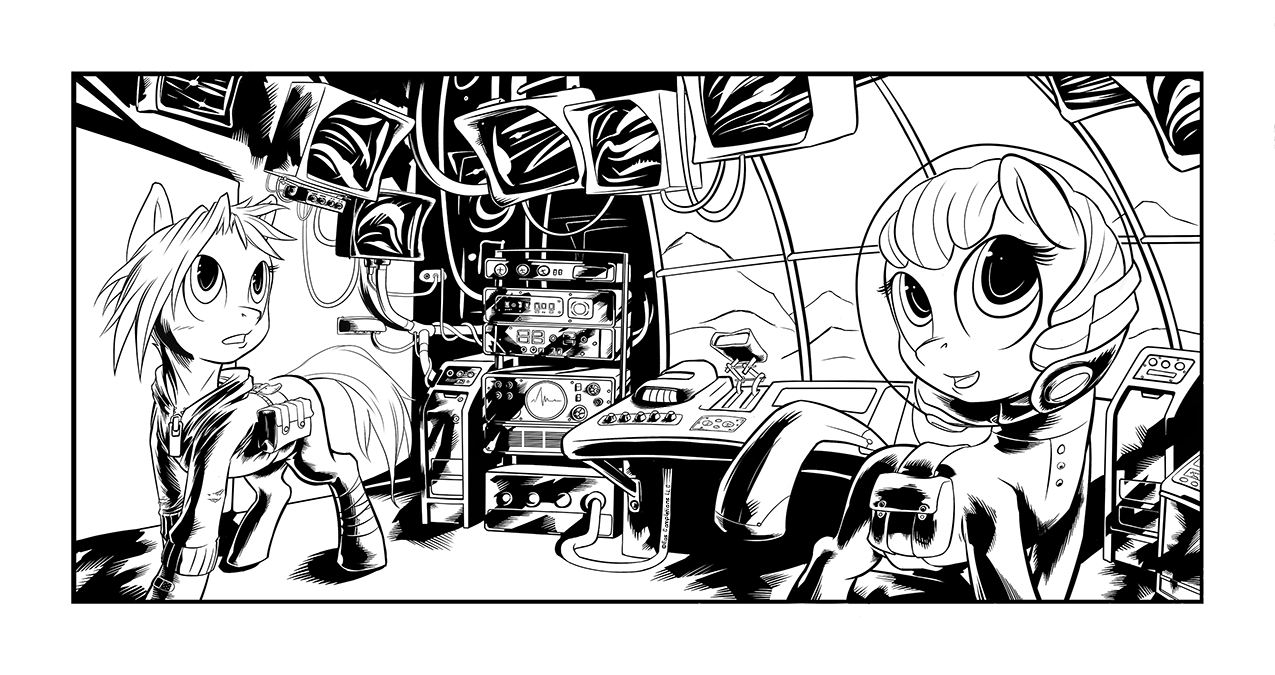
\includegraphics[width=0.9\linewidth]{image08.png}

\begin{intro}
那些床底下的黑影总让我担惊受怕。
\end{intro}

\daytimeplace{7}{3:00 AM}{旭日隧道,隧道镇}{Solaris Tunnel, Tunnel Town}

打了个哈欠,扳机低头看着幼驹在控制室地上玩。帕比正在一边用嘴发出『嘟嘟』声一边玩着一辆玩具车,她把一堆瓶盖放在车上,然后卸到一个闪闪可乐空瓶子边,然后再把瓶子装在车上。

「可以给我超级特别薄荷口味吗?好,谢谢,再见……」幼驹小声地玩着,好像她担心发出噪声惊扰到其他小马……

\thpr{她怎么做到的?把所有那些烦恼都丢在一边,然后就那样……坐下来玩儿?像个普通孩子一样?}

「喏,小家伙,你朋友怎么样了?」

帕比一边继续玩着她的玩具一边回答:「不知道,她说要花好一阵子呢,所以我要在这里等她……」现在幼驹似乎在用什么做一个围栏。

扳机吓了一跳,「你怎么还带着 \SI{9}{mm} 子弹?」

「哦,那些啊?闪闪发光的漂漂东西,而且好像有个揪耗毛兽强啥的要用。」小雌驹埋头玩着玩具。

「啥啥啥?」

帕比伸起蹄子大喊着:「吵吵的东西!」一把破破烂烂的九毫米半自动手枪出现在她蹄子上,吓得扳机连忙躲到一台终端后面。

「喂喂,谁给你那玩意儿的?很危险的!」

「才不,这东西吵死了……我也不喜欢,只有小雄驹才喜欢这种玩具的啦,除非它是粉色的话……」

女卫兵紧张地笑着,「对哦,帕比,那东西一点都不好玩,想换点有趣儿的东西么?」

这句话引起了帕比极大的兴趣,幼驹转过头来,水汪汪的粉色双眸闪闪发光,满怀期待的看着扳机。

「当然啊!你有什么?」

「呃,一个墨镜\footnote{墨镜:带墨镜的卫兵……黑杰克躺枪}如何?」

「好耶,墨镜!等等……」帕比皱起眉头,「我戴着这破头盔,戴不了墨镜的。」

扳机以蹄覆面,「好吧,抱歉小家伙,我想什么呢。」独角兽回头在她的鞍带里面翻着,「那么这本九成新的《缰绳八卦》杂志如何?里面全是漂漂马照片,还有小蝶的!」

帕比走到卫兵身边,看着杂志,然后开心地一蹦老高,「我喜欢这个,里面全是漂漂马!我认识这个,她是萍琪派!还有瑞瑞!哦哦,云宝黛茜!我超超超喜欢云宝!她可以飞在天上嘣嘣嘣!等我长大了我要当她的新娘子!我喜欢这个画册,给我嘛给我嘛给我嘛!」

扳机举起蹄子掩着自己嘴角的窃笑,「我想我们可以成交了,不过你要把子弹也给我。」

「好好好好!哦哦哦!这个大的子弹你能换给我什么?」帕比问着,又掏出一发大号的坦克用尾翼稳定脱壳穿甲弹头。

独角兽雌驹叹了口气,事情越来越麻烦了。

\horizonline

\daytimeplace{7}{3:00 AM}{糖霜咖啡馆,隧道镇}{Sugartop Cafe, Tunnel Town}

昏暗的咖啡馆里面现在烟雾缭绕,和每天夜里的这个时候一样,完全是个颓废的地方。几个醉醺醺的小马东倒西歪地躺在那里,吸着来历不明的药品,一只狮鹫躲在房间的角落,还有一只戴着墨西哥帽子的小马在弹七弦琴。酒保正在用一块黑得看不出颜色的抹布「清理」着地板,但是坏枪根本都不在乎这些。

「再来一杯!」他摇摇晃晃地举起空杯子,用力吸着里面的蓝色吸管,但是却发出空荡荡的吱吱声。「我说,你聋了么?我说再来一杯!」他不停地晃着酒杯但是谁也不搭理他,真是失望。

这里的酒保,那只黑鬃的银色公马,坐在他旁边放下一瓶闪闪可乐,「我说大家伙,安静点,客人在楼上睡觉呢!」

「闭嘴!老黑!」坏枪嘟囔着,「赶紧给我倒点儿给力的玩意儿,我真不敢相信她居然甩了我!」

年轻的伙计叹了口气,把可乐瓶推到坏枪嘴边。「拜托老兄,别惦记她了,赶紧睡觉去,你可以睡我楼上的床,别喝了,一点用都没有。」

卫兵看着他兄弟的脸,但是却不想从桌子上抬起脑袋来。

「你知道这酒吧有一半是我的么?」

「对,但是你每次来就是和我抱怨你过得有多悲催。然后呢,处理顾客,打扫卫生,撵走不付钱的醉鬼……」黑帽子在桌子上敲着蹄子,「老实说你帮我做了哪样?话说你自己就是个不付钱的醉鬼好么?」

坏枪挥着蹄子像是赶苍蝇一样嘘着他的兄弟,「滚边儿去老黑,你的臭气都快把我熏昏过去了,给我点新鲜空气。」

「那你为啥不去城外走两圈,好像坐在这里就会空气好一样。」

「闭嘴,再给我倒杯性感天马,老黑……」坏枪举着空杯子,脸却扎在桌子上。「她怎么可以……」

终于黑帽子发火了,「拜托,老兄,我知道你在说谁!就是那个快乐扳机,这是我见过最烂的婊……」

砰!

坏枪看着他趴在地上的兄弟,「老黑,你还真说错了,呆这里鬼混让我感觉到……嗯……非常好,」公马说着往外走,「谢了老弟。」

\horizonline

\daytimeplace{7}{3:15 AM}{旭日隧道,隧道镇}{Solaris Tunnel, Tunnel Town}

「帕比,你还记得……小马国两百……呃……在你离开中心城之前,那里怎样?」

小雌驹皱着眉头,想要想出个答案来。「新鲜!」

「新鲜?」

「没错,妈咪好像是某种士兵,但是她其实不喜欢打仗,她很擅长修东西,所以不是很危险的时候她都带着我。我见过很多神奇的好地方,比如说一个天马机场,还有地底下的一个叫避难厩的大地洞,但是完全不知道那是什么……而且我还到过小马镇,还有其它很多地方……」幼驹很自豪地抬头挺胸说:「不过52号国道的小马们看起来好可怜,这里没有青山绿水,也没有漂漂房子,小马们也都很不开心的样子。」

扳机感觉到有什么东西哽在喉咙里面,「如果……如果你不想说的话……就别说了。」

帕比看着独角兽,有些奇怪地回答:「为什么不想?虽然这里不如其它地方漂亮,但是这里也有很多大姐姐一样善良的漂漂马……或许等我找到妈妈可以带你去看那些漂漂地方……真的!我不知道为什么你们喜欢住在这种灰扑扑的地方。」

「呃……当然可以……不过……你可以先和我说说小马镇么?」

「当然!那可是我见过最漂亮甜美的小镇!那可是萍琪派去中心城之前住的地方!妈咪因为要去做很重要的事情所以让我在那里呆了整整一个暑假!我在那里交了好多朋友!而且那里的山丘和树木颜色都非常漂漂。哦哦哦,还有一个叫旋转木马的地方!但是并不是真的旋转木马,只是名字……」帕比皱了皱眉头,「我只告诉你哦,因为那个时候我问为什么那里的木马都不转圈圈,大家都笑了,而妈妈也抱起我笑,不过我却觉得自己超级蠢……所以……别问我为什么木马不会转哦。」

扳机咯咯笑着点了点头:「别担心,我不会问的。」

「然后那里的苹果园中间还挖了一个超级大超级大的水洞。哦哦,那里还有一个城堡一样的云屋,上面还有彩虹瀑布落下来!对了,还有个商店卖羽毛笔和沙发!」帕比看着扳机的表情,担心地问:「乐乐姐我说错了什么吗?为什么你哭了?」

「我……我没哭,只是眼睛进了东西……」

「哈喽!都给我乐起来,小姐们!P7来啦!」忽然房间里面的所有屏幕都变成了粉色,每个屏幕上都出现了好像七个气球捆一起的标记。

「你好,声音小姐!谢谢你能过来!」帕比对着最大的屏幕挥着蹄子,那里的气球已经被一行字代替。

「多谢你给我找的新家,帕比!这里比那个到处漏风进雨的破圆顶好多了!我们看看这里有什么……哦!地热发电机!维护机器马离线……这个简单……哦哦!还有好多好多秘密文件还有……呃……红色安全警报?我怎么忘了这东西?」声音暂停了一会。

「有什么不对吗,声音小姐?」

「没,只是我需要旭日公司的某个大头头的授权来解除警告,不过好像已经有某小马在程序上开了后门,所以我可以简单地绕进去,一会儿就搞定!」

扳机有点狐疑地看着屏幕,她从来不喜欢A.I.,但是这个看起来很友善,帕比也认识她,所以她决定还是等等看发生了什么。

而帕比已经完全放松下来了。小雌驹和往常一样天真灿烂地笑着蹲坐在大屏幕面前,「好的好滴,你现在能找到我妈妈是不是在附近么?超超拜托?」

「红色警报解除!所有系统正常,安全门即将打开,5、4……哦,我不知道帕比,这里的主机是个巨大的数据库,而且没有授权的话我不能……哦哦等等……我在这里找到『那一天』之后三个星期的数据……不过我需要一个密码……」

小雌驹举起蹄子,「我知道!快乐帕比!」

扳机叹了口气,「帕比,你的名字不可能解开所有东西,你知道……」

「密码正确,虽然这东西都放了有两个世纪了,我把它们显示在大屏幕上。」

幼驹皱着眉头颠过来倒过去地把这几行字看了几遍,然后泪汪汪地转回头来。

「帮帮忙……」

独角兽雌驹坐在帕比身边,然后用蹄子轻轻搂着她的脖子,「当然小家伙,我读给你听好不好?」

\medskip

\begin{center}
\textbf{第十八天}
\end{center}

\wrpr{如果我还有向塞拉斯蒂娅公主祈祷的权力的话,我真希望避难所科技的那些书呆子来做这些工作,而不是旭日公司的这群}

\medskip

% NOTE: 译文错误

「呃,骡子,没错帕比,就是骡子……」

\medskip

\wrpr{这傻蛋旭日公司还真搞出一个在紧急状况下把优先权赋予技工的协议。但是这帮蠢货居然忘记给机器卫兵设置敌我识别!}

\medskip

「呃,这个词没啥意思,帕比,我们继续……」

\medskip

\wrpr{至少隧道现在还安全,我会在这里扎营几天,然后收集一下补给品为穿越沙漠做准备。}

\wrpr{已经快凌晨两点了,但是我睡不着,我好想她!我知道她在避难所里面很安全,但是我还能听到她因为怕黑和做恶梦拼命叫我的名字,但是我醒来却发现只是个噩梦。}

\medskip

「胡扯……嗯,是的,胡扯。」

\medskip

\wrpr{我应该给自己找点儿事干,免得我发疯,我恨小马国}

\medskip

「嗯,这部分是向女神的小小祈祷。」

\begin{flushright}
\textbf{阴雨·黛丝}
\end{flushright}

\medskip


扳机叹了口气,\wrpr{阴雨·黛丝女士写这个的时候,她绝对没想到她的小女儿真能读到这个东西}。

「好吧,看起来她继续往南走了……我们继续看看下面的记录。」

P7打断她们的对话问道:「喂,帕比,你记得沙盒主任的密码么,超超拜托!」

幼驹戳着自己的头盔思考着。「玛塔莎?不对……是阿加莎!」

「谢谢啦,亲,我超超超想给你个大拥抱,让我们做做看吧,你先抱一下你自己,然后就当是我抱的好了!这里还有第二个文件,我会去我不该去看的地方转转看,你们好好玩儿,别弄得一团糟哦。」

\medskip

\begin{center}
\textbf{第二十一天}
\end{center}

\wrpr{我终于准备出发了,看起来没有其他小马来这个方向,我难道是这里唯一的幸存者?不太可能,但是我不想赌自己的运气,我打算绕开太阳城,这里被核弹头密集轰炸过,昨晚我都能在沙漠中看到那诡异的辐射光。如果我走运的话,几天之后我就能走到蓝羽机场了。我一天亮就出发。}

\wrpr{我还是睡不着,我一直梦见帕比死在厨房的地板上……}

\medskip

「胡扯,帕比,胡扯……」

「你喜欢胡扯么?」

「好了好了我继续读……」

\medskip

\wrpr{这只是噩梦,我很确信她很安全,她从来没有不听话过,为什么我一直梦到她?我找到一些药片,其中一些可以当安眠药,如果再做噩梦的话我就吃点儿。}

\begin{flushright}
\textbf{阴雨·黛丝}
\end{flushright}

\medskip


帕比紧紧地抱着卫兵,头盔紧紧压着扳机的后背。

「怎么了小家伙?她只是想你了,你现在好得很,等你找到她之后你就没事了,她也不会做噩梦了,对吧?」

和幼驹扯这种毫不羞耻的谎话让扳机的内心如同刀绞,但是帕比现在需要安慰。

「我……我不是好孩子,乐乐姐……我没有去那个秘密地方,因为我想去看烟花!」幼驹大哭起来,「我是坏孩子,妈妈会生我气的!」

扳机转身抱起小雌驹,安慰着她,「好了好了,别担心,你妈妈说了她要往南走,对吧?去一个……什么蓝羽机场?……我想那里就是铁锈庄园了,去那里很简单,只要绕过太阳城就到了,她再见到你一定很开心的!」

\thpr{为什么我要给这个可怜的小家伙希望?她妈妈早已经死了,我到底在做什么啊!}

那双清澈的粉红双眸中燃起了新的希望,帕比凝望着雌驹,「真的?她会在那里吗?」

「我……我也不知道她是不是,不过你想要追上她吧,对吧?如果你想要寻求真相,你必须跟着她新的足迹继续前进!」\thpr{没错,乐乐,两百年前的新足迹。}

幼驹又一次笑了起来:「对!我去什么地方都没关系,跟着妈妈,我去什么地方都可以!谢谢你乐乐姐姐!你是最棒的小马!」

P7又一次打断了她们,「非常好,我搞定这里的物品清单了,好像旭日公司的家伙早就开始为『小马国末日』做准备了,这里有好多实验室,而且还有足够的军火再给那些幸存者来一次烟火秀!哦哦,帕比,我想你刚才又把萍琪派的名字给念错了!」

帕比抬起了头,「啥米?」

「简单的说,朋友,在这个山下面有好多好多层仓库,装满了各种军火,那些东西足够把小马国上的每一个混蛋都杀死两次!」

「呃……你说『杀死』是说,伤的很重?」小雌驹狐疑着问。

「不对不对!我是说伤得超级重!就像一个所有小马进去以后就出不来的超级大派对!」

「一个……机器萍琪派对?」帕比不由得打了个寒战,完全不想听到之后的回答。

「机械萍琪:文件未找到。」

帕比想了想然后又问:「好了,那么这些东西有些什么呢?」

「我们举几个例子吧!比如说『长程多弹头电浆导弹』这玩意能分裂成56个弹头同时命中56个不同的目标,每个弹头都可以轻易击穿地下防御掩体,然后把整个密闭空间灌满电浆,把温度瞬间上升到几千度,杀死里面的所有小马!还有『广域解离射线发生器』,可以把一百米之内的所有目标分解成原子状态,当然也会杀死小马。哦哦,还有『巧克力混沌\footnote{巧克力混沌(Chocolate chaos):正剧 S02E01,无序躺枪}』这个魔能武器可以把目标的血液变成巧克力牛奶!虽然效果会在一个半小时后消失,不过被打中的马当然也是立刻就死翘翘啦!」

「好了好了,不用说了……」帕比打断她的话。

「那么,我们该怎么办?你是老大!」

电脑最后一句话的话音刚落,扳机连忙举起蹄子想阻止小雌驹说出任何蠢话,不过她还是不够快。

「把它们全扔了!挖个大洞把那些东西都丢进去,在上面盖个房子然后把这里的所有坏蛋机器都送进去,这样就不会有小马受伤了!」

「好吧,从技术上讲,所有东西已经在这个山下面的大洞里面了……我可以炸毁通向仓库的电梯,除非有谁把整个山都挖开,否则他们肯定找不到那些东西了。」

「就这么办!」

扳机松了长长一口气。

\horizonline

\daytimeplace{7}{3:30 AM}{隧道镇,52号国道北口}{Tunnel Town, Big 52 N Branch}

坏枪用头撞着隧道的大铁门。

「肏,肏,我应该阻止她的……肏,肏,肏肏肏!」

「我说,老哥,就算你用力踢它,门也不会奇迹般地被你踢开的。」黑帽子坐在卫兵身边揉着眼睛,「我想这个乌眼青是我自找的,不过……这不代表我哪天会打回来。」

「看在露娜的份上,老黑!拿个腌青鱼压着那眼睛睡觉去,让我自己静一静行不行!」

银色公马靠在墙上打着哈欠,「没门儿,我才不会把我兄弟丢在这里,而且,这件事足够我笑话你几个月了。」

坏枪怒气冲冲地喷着响鼻,「我总怀疑我们老妈是个婊子,现在我很确定了,乐乐都已经不在了你还想笑!你是想再多个黑眼圈还是现在就滚蛋?」

「冷静点吧,你现在啥也做不了,这东西封得……我勒个去!」

一阵尖锐的金属摩擦声之后,大门缓缓升起,让黑帽子一屁股坐在了地上。

「我勒个大去……」

俩小马一脸难以置信的表情看着巨大的钢铁怪物——两米厚的巨大防水板慢慢升起,然后后面的另一扇隔板也缓缓让开。

坏枪傻站了快一分钟才张开嘴。「这……我……没做梦吧?掐我一下……」

砰!

「你这个尸鬼养的……我是说掐一下!」

老黑窃笑,「我说了你欠我一下,你还说她已经死了?」

两只雄驹蹄下跨过骷髅走进山洞内,黑帽子看着满是子弹孔的马车,又看着里面装的东西。「哇哦!这么多好东西!这小镇要发财了!」

坏枪则稍微走得远了一点,看着隧道的灯一盏一盏点亮,开始照亮这六公里长的地下隧道,而天花板上的一处通风道还挂着一根绳子,于是他撒开蹄子飞奔向山洞深处。

「等等老哥!别跑那么快!我们要叫上其他卫兵!」

「去你妹的卫兵!我喝高了而且还恋爱了!」雄驹的声音回荡在隧道中。

黑帽子叹了口气,跟着一起追了过去,「至少你等等我呀!」

\horizonline

\daytimeplace{7}{9:00 AM}{隧道南贸易站,52号国道中段}{Trade Station Tunnel South, Big 52 SC Branch}

扳机抱着帕比亲着她的头盔,而后者一脸不耐烦地拼命挣扎着。「唔……好肉麻,别在那么多小马面前亲亲!」

所有城镇卫兵和隧道镇的许多其他居民都围住了他们。在扳机护送着帕比走出隧道南口的时候,一位代表小镇政府的雌驹发表了一个小演讲,并且送给帕比一袋子瓶盖。

在两只小马面前是无边的地平线无数的沙丘,偶尔有几个红色的山石出现在视野中。在远处能够清晰地看到一个城市的剪影,但是沙漠的风尘让大家难以辨识这是真实的景象还是海市蜃楼。

「帕比,我们到了,这就是蛇蝎沙漠,你好好听我说怎么去铁锈庄园。」

小雌驹乐得蹦蹦跳跳的,「没问题,漂漂乐乐姐!」

「很好,这个荒漠是清砂工的领土,他们大多都是住在各种各样帐篷的拾荒者,在沙丘下面寻找各种有用的东西,不过我还是要提醒你,他们有时候还会抢劫,尤其是对于独行的旅者,但我觉得他们恐怕没那个胆子敢抢劫你,毕竟清砂帮是个非常迷信的氏族,而且他们肯定从孤狼那里听说过你的事了。」

帕比点了点头,「喜欢走来走去的漂漂马,懂了!」

扳机笑了笑,「很好,你只要跟着路标,很简单的,因为每隔50米清砂工就会放一面红色旗帜,你只要跟着旗子走,就能在明天早上之前到达他们的第一个营地。」

帕比皱着眉头指着旁边坚实的柏油马路,「为什么不走大路?踩着我的滑板在路上就像飞梭一般!」

「不行!小家伙,这个公路是直接通往太阳城的,你绝对不能去那个地方!」

「为啥?」

「那里是个危险的地方,所有小马去那里就再也没回来过!」扳机的声音中带着不容置疑的口吻,但是帕比完全没有在意。

她敲着自己头盔下巴的位置,「呃,或许他们超喜欢那里,所以不想走了呢?」

「我……我可不觉得……帕比,当我还是你这样的孩子时,太阳城是另一个氏族的地盘——锈刃,他们和清砂工是同盟……那是很久之前的事情了,但是后来听说清砂工找到了什么大家伙,而锈刃偷走了,然后就是说谁背叛谁的,最后他们就打起来了。最终清砂工想要策划一次突袭,在晚上夜袭城市。」雌驹顿了顿,看看幼驹还有没有在听。

「然后呢?」小听众有些担心地问。

「在突袭中发生了什么灾难,但是谁也不知道究竟出了什么事,只知道清砂工带了他们的所有武器冲进城市,但是却谁也没有回来,所有想要调查城市的小马都消失了,然后清砂工把剩下的小马聚集起来——大多都是老马和孩子,现在还在沙漠中挣扎求生。」

「所以,他们都是大坏蛋?」

班级皱了皱眉头,「在废土可没有什么明显的善恶之分,帕比,如果你想活下去,有些时候你必须做出一些……牺牲……就算是心碎也好,总比彻底失去生命要好。」

「呃……啥?」幼驹一脸茫然地看着扳机,不知道她话语之中的哲理。

「好了,别瞎想了小家伙,你就觉得……好吧……他们是坏蛋,但是他们不是自愿的。」

帕比摇了摇头,「不对!如果你做坏事,那你就是坏蛋!没有借口,如果觉得小小坏事就不算是坏事,那你最后就会做出大坏事,变成一个超级……超级大坏蛋!」

「呃……你自己想出来的么?」独角兽钦佩地看着帕比。

「才不是咧!妈妈说的!」

扳机拍拍帕比的头,看着她担心的表情,「别担心,打烂机器马不算坏事,妈妈不会不开心……好啦,笑一个!」

黄色的幼驹开心地跳上滑板车,「我见到妈妈以后会告诉她你对我超级好!谢谢你漂漂乐乐姐姐!」骑着滑板车,幼驹顺着沙漠的公路绝尘而去。

「呀呵呵……」

扳机看着幼驹骑着滑板越来越远,然后叹了口气,「我很抱歉,小家伙。」

「那么,乐乐,那就是那个小幽灵?」坏枪走到雌驹身边笑着问。

「我不知道,」扳机叹了口气,「我只知道她是个迷路的孩子。」然后她转头看着公马笑了起来,「你那熊猫眼哪里来的?」

「兄弟情谊纪念。」坏枪哼了一声,然后又说:「我们何曾不是迷失在这个残酷的世界之中呢?不过我想新闻一发出去的话,很快就会有大批小马来隧道镇了,我们要增招卫兵。」

「说到那个……马车上的货物应该回收,那些东西应该平分给每个小马,你帮我看好黑帽子。」

公马点了点头,「没错,别担心,其他小马已经把车拉回城了,有些车还是有标志的,有三个属于水头,还有一个是旋转木马的,不过上面的东西已经被和机器卫兵对干的小马糟蹋得差不多了。我们还给他们吗?」

「我们应该还给他们,至少作为我们善意的象征,他们知道我们帮他们保管好货物的话,也会乐于和我们合作的。哦,顺便提醒了我要教教你如果通道再次关闭的话该怎么打开。」

坏枪迟疑了一会之后又追问道:「还有,那个……昨晚那个……你知道的……在你追那个幽……帕比之后,我和你说了些……然后我们……能假装……我们什么也没说么……你知道的……那个……啥……」

扳机咯咯笑起来,「我可不觉得,大情圣……那可是我见过最笨的告白了,为了那些话,我也要和你过下半辈子啦。」

坏枪低下了头,「呃……我可以问问为什么吗?」

「我可以先问你一个问题么?」

公马挥着蹄子,「当然……问吧……把爱心之箭射入我心房吧……」

「我还有机会说……我也爱你吗?」

\horizonline

\daytimeplace{7}{4:00 PM}{蛇蝎沙漠,52号国道中段}{Serpent Desert, Big 52 SC Branch}

{\rt 女士们,先生们!下午好!这里是孤狼的52电台!小马国这片区域最好也是唯一的电台!昨天我正在街上走然后有小马问我,为什么大家都听你的节目?你的节目怎么会这么好?好吧,我必须承认那个不简单,因为我可是这附近唯一一个肏蛋DJ了。}

喇叭里一个女性在远处说:「{\rt 耶!!没错!}」

{\rt 坏孤狼,你说脏话了!你不应该说脏话的!尤其是我们的小英雄还在听你的节目的时候,对吧,对吧!我是个坏蛋我应该害臊才对。不过现在我却觉得很高兴,不,是非常高兴!因为一个带翅膀的朋友刚给我从南边带来了大新闻!做好心理准备,听众们,因为这个新闻超级劲爆!}

忽然随着一阵静电干扰声,广播中断了几秒钟,但是马上就恢复了。

「{\rt 好了,听众们我又回来了!你们竖起耳朵听好!谁也关不掉52电台,特别是今天,因为今天我们要一起庆祝隧道重新开张!没错小马们!你们耳朵没撒谎!隧道镇又回来了!再也不用走山路了!}」

狂野的音乐持续了一分多钟,而DJ在背景里面用嘴模仿着吉他的声音。

「{\rt 这可是砸烂嘉年华之后最大的好消息,猜猜是谁干的?没错,我们的守护天使!我们的小小幽灵!我们需要一个小孩子把我们从濒临饥荒之中拯救出来吗!肏你妈我太失望了!不过不开玩笑,一个小孩子,一个星期不到的时间,就把三个城镇从他们最恐怖的噩梦之中拯救出来了!一个小孩子而已!我说52,你们的骨气都哪儿去了?给我看看你们的信念!别让我一直崇拜一个比我小好多好多的小孩子行不行?}」

一阵沉寂之后,DJ的声音又回来了,这一次显得疲惫不堪。

「{\rt 醒醒吧伙计们,她只是一个孩子而已,她不可能搭救所有的小马,我们应该振作起来,我们自己就可以做得更好,我们不需要另一个英雄来崇拜!}」

一段悠扬的吉他声之后,另一段音乐响起,不过这次不是录音,而是孤狼自己唱的歌。

\begin{music}
走出废墟,走出残骸

Out of the ruins, out from the wreckage

\medskip

我们不能再犯同样的错误

Can't make the same mistake this time.

\medskip

我们是新一代的子女

We are the children, last generation.

\medskip

我们是被遗忘的一代

We are the ones they left behind\dots

\medskip

我们要改变这个时代

And I wonder when we are ever gonna change it,

\medskip

在恐惧和余烬之中挣扎求生我们一无所有

Living under the fear till nothing else remains.

\medskip

但是我们不需要更多英雄

We don't need another hero\dots
\end{music}

\horizonline

「哇哦,我真想见见他们说的那个超级英雄小雌驹!你觉得我们可以做朋友吗?」帕比跟着红色旗子在沙漠上走着。

「{\mt 肯定,通常英雄偶像都是相当友善的。警告,检测到中等辐射,威胁等级:可忽略。}」

幼驹一边走着一边问着:「对了,声音先生,你觉得我是好孩子吗,我妈妈还喜欢我吗?」

「{\mt 警告,该程序没有社交功能。}」

帕比长叹一声,「老天,每次问到关键问题你就躲起来,是吧?」她正想在说点什么,但是她的注意力被远处一个影子吸引了,「看,有个漂漂马!」

这个「漂漂」马看起来是一只鬃毛花白的红色独角兽,一件宽大的披风遮盖住了她的全身。当小雌驹走近的时候,她笑了,「慢慢来,小幽灵,我在中午就在这里等你了。」

「嗨,我是快乐帕比!」小雌驹挥着蹄子笑着说:「我很抱歉我迟……呃,我哪里迟到了?」

老马的嘴角微微挑起,「当然是探险……你喜欢探险吗?」

「是啊!我超超超爱探险!哪里可以探险?我能来两个吗?」忽然幼驹的表情变得严肃起来,「不对……等等……我还要找妈妈,不应该去探险……」

老马笑了笑,「没错,你已经有自己的路要走……我怎么忘了这个。」

帕比点了点头,「没错,我很抱歉,我该走了,谢谢,拜拜!」

「不过,如果我说这次探险是关于你的一个陷入危险的朋友呢?」

已经走开的幼驹又回过了头,「我的一个朋友?谁啊,为什么,在哪儿,什么时候?」

「好了,别急……」

帕比跳上长者的后背,用她的头盔贴上了她的鼻尖,她紧盯着独角兽的眼睛。

「拜托拜托快跟我说!」

老独角兽一下子没站稳,差点摔倒,「冷静一下,小幽灵,我正打算和你……快坐下听……好不好?乖乖的我就和你说话!」

「呃……好的……很抱歉漂漂老奶奶……」帕比放开她的脖子然后坐在独角兽面前,而后者松了一口气。

「我是先知长耳,一个可以看到远处景象的小马。」

帕比蹦蹦跳跳地说:「哦哦哦,你能看到我妈妈么?她能看到我们吗?她还好么?」

「不是那样的。」

小雌驹一瞬间泄了气坐了回去。

「我吃一些药之后,我可以在梦中看到一些景象,但是我不能选择我要看什么,昨晚我看见的是关于你的梦境。」

帕比安静地坐下来,在沙漠当中听着长耳慢慢讲故事。

「你让一个非常重要的朋友为你做一件很重要的事情,你的朋友竭尽全力,但是发生了一件非常糟糕的坏事,她没法再继续她的任务了,所以她在我的梦中让我来转告你。」

帕比皱了皱眉头,一个很重要的朋友帮一个大大的忙?但是她从来没有——哦哦,是丝尾!她让它照顾赫瑞别让坏事发生在她身上!

「赫瑞?她有危险?在哪里?」

雌驹点了点头,用蹄子指着远处的太阳城,「我恐怕那只小鹰飞得太靠近太阳,所以找不到回来的路了。」

帕比犹豫了一会,「但是……乐乐姐告诉我不能去那里!我要听她的话!」

长耳耸了耸肩,「你并不是非去不可,你让朋友帮忙,而她让我警告你,就是这样,你可以选择不管她,然后继续你的旅程。而我的任务也就是这样。」

「但是……但是有什么坏事发生在赫瑞身上!我不能把她丢下!她可能会受伤!她可能会哭!」

「那么,去太阳城救她吧,但是我要警告你,太阳城是一个陷阱,是个真实的噩梦,当你开始做梦之后,你就不能再离开了。」

「这个别担心,我一点都不困!」帕比笑得别提有多轻松了,「太空战士安德洛队长前去营救啦!」幼驹向城市奔去。

长耳看着飞奔的黄色幼驹,直到她远到化成一个灰色的小点儿,然后拿出一个药片,就着一瓶奶白色的液体吞了下去。但是老马能看到的只是火焰和枪声,

「我看到的是什么?过去还是未来?」

咯咯笑的声音在老马耳畔响起,「她很精神,一直在笑,我喜欢她!如果大家都能像她这样,不是一直板着脸的话……」

母马低语着:「但是一个梦魇能带来和平么?我不确定……」

「别问我啦!我只是你的迷幻剂带来的一个幻觉而已!真的,我帮不了你什么!就算你不看它,事情也会发生,而且你也不知道这个是过去还是未来。」

老独角兽叹了口气,「或许你是对的……我们回家吧。」

「对,我们走吧,帕比会照顾好自己的!」

\clearpage

~\vfill

\begin{note}
升级(Lv 7)

新技能解锁:钢铁力量——有时候光是石头还不够,你使用的所有钝击武器都增加5点额外伤害(没错,石头和动力蹄都属于钝击武器)。

任务技能:52之魂——你的传说在52号国道上流传,只要大多数氏族和你的关系保持中立或者中立以上,你随机遇到的低级敌对目标就会减少。
\end{note}


\chapter{太阳城}

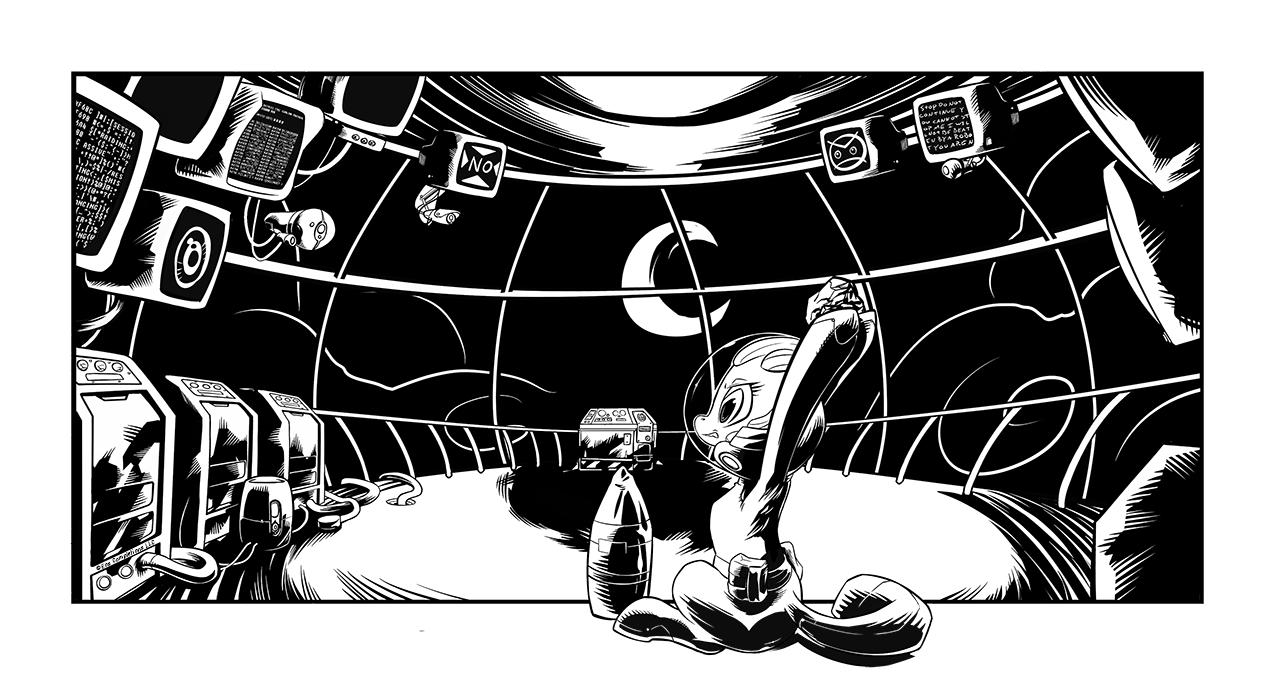
\includegraphics[width=0.9\linewidth]{image09.png}

\begin{intro}
太阳城不只是一个小镇,它是小马们罪孽的救赎。
\end{intro}

\daytimeplace{7}{11:00 PM}{太阳城郊外,52号国道中段}{Sun City Suburbs, Big 52 SC Branch}

去城里的路非常远,帕比走到第一个房子边的时候,夜晚的黑暗已经笼罩了街道的每一个角落。太阳城中心社区被一大堆小小卫星城区包围着。但是每个窗户都黑漆漆一片,半点光亮也没有。帕比走过的建筑看起来都已经被拾荒者洗劫一空,只剩下一个个房子尸体般的空壳,就像是一片坟墓,一片曾经被叫做「家」的东西的坟墓。

帕比并不想承认她还有点怕黑,但是这个空旷的地方让她想起来小时候的各种鬼故事,「为什么小鸡要跑到这么可怕的地方惹麻烦?笨赫瑞!这里什么都没有,为什么还叫『城镇』?」

随着深入这个可怕的地方,帕比开始好奇,那些五颜六色的标志都去哪里了?虽然她没怎么在夜晚出去过,但是她很确定夜晚的城市不是这个样子……她想要一些音乐以此盖过夜晚阴风吹过空洞房屋发出的哀嚎,但是无线电一到太阳城附近就没有声音了,让帕比感觉到又孤单又害怕。「呐,声……声音先生……你还在吗?」

回答帕比的只有一堆毫无意义的沙沙声。

「{\mtzh 兹兹……危险……沙沙沙……变……兹兹……电……沙沙沙……可能\\……哔哔……影响……哗哗哗……思考。}」

% NOTE: 强制断行

「唉,他又生气了……」幼驹皱着眉头继续走着,头盔的HUD开始显示文字的警告信息,但是密密麻麻的字幕活像是蚂蚁,而且滚动速度快到帕比根本没办法看清。小雌驹觉得自己孤立无援——无线电坏了,声音先生不见了。就像那些可怕的夜晚,她想要睡觉但是屋子太黑太可怕,她不停地叫着妈妈,直到妈妈过来抱起她抚摸着她,把她哄安心。帕比想要唱点儿什么壮胆,但是在这种黑漆漆的地方她只能想起「邪恶女妖」啥的歌,完全没有什么帮助。

帕比走过迷宫一般空旷的街道,蹄声的回音让她觉得毛骨悚然。每一个空洞的窗户都反射着她双眸里明亮的粉色鬼火,那是什么?或许马尾伯爵又从坟墓里面爬出来了?而且她觉得这个时候就连马尾伯爵都不那么可怕了……远处传来一阵不可状名的尖叫声吓得幼驹僵立在原地,她后蹄一软直接坐在了马路上。

「那……那……那……那……那……那……是啥?」

打烂坏蛋机器和追着妈妈一点都不可怕,而尸鬼小马虽然看起来很惊悚但是她至少知道自己可以打什么……但是这里完全不一样——一个空无一物的城市,到处都是闹鬼的房子和发出怪声的街道,她为什么想到鬼怪幽灵?不要幽灵!坏幽灵!为什么她要离开红旗子的小路,漂漂姐姐明明说她不要离开那条路,但是她必须来这里帮那个笨小鸡。但是现在这里又黑又可怕,帕比超想念丝尾小姐。

小幼驹趴在路上耷拉着耳朵,尽力假装自己是路上的一块石头。

「新……新……新……新……计划!我们在这里等明……」

另一阵声音在空旷的街道回响着,好像是幽灵的哀嚎一般。

「……天……啊啊啊啊呀呀呀呀!」帕比撒开四蹄,风驰电掣,就像在落叶赛跑上的云宝黛西那样一溜烟飞奔出去。

「新计划!我们出城等天亮!」

\begin{center}
太阳城1分——帕比0分
\end{center}

\horizonline

\daytimeplace{8}{8:00 AM}{太阳城郊外,52号国道中段}{Sun City, Big 52 SC Branch}

天亮之后,这个城市看起来和盐块城差不多,甚至比得上中心城,一点儿也不可怕……就是有点儿……呃……丑。帕比在想为什么昨晚自己那么害怕,她真是个笨小孩。

「看吧,声音先生,这里没什么好怕的!就是另一个城市,到处都是破房子和烂马路还有……」帕比忽然看见有什么东西从头上飞过,「还有漂漂翔马们\footnote{翔马们(Peggysuses):天马这个单词的复数就连很多英语母语的人都会搞错}!好棒!」

幼驹撒欢跑了起来,追着那个飞行的影子。「喂!喂喂喂!漂漂翔马们等等我……等等噗……」抬头看着天跑的小幼驹完全没有看前面,径直撞进另一个走在街上的陆马怀里。

「哎呦……你为什么不看路啊!我先从这里跑的!」

那个棕毛黑鬃的成年陆马似乎正背着一大堆砖块和其它建筑材料,不过现在已经被帕比撞得散落一地,帕比心中一惊然后立刻打算在那个老马生气之前溜走,但是他只是低头开始默默地把砖块捡回去。

「哼!这下知道教训了吧……别站在路中间和一个笨雕像一样!」帕比吐出舌头做鬼脸,但是她发现那个陆马根本没有在意她。他看起来只是有点……怎么说……

「呃,抱歉先生,您没听到么,我是快乐帕比,我在找我的妈妈……虽然通常是这样,不过今天我是来救我的朋友赫瑞,听说她在这里惹上麻烦,但是我又不知道是什么样的麻烦,你有看到她么,她有一个喙而且长着毛,看起来像是一只小鸡但是又不喜欢我叫她小鸡,但是我叫她小鸡又不是她想的那个小鸡,不管怎么说她都看起来像是小鸡,对了哦,我还见过斑马,我不知道为什么小马都不喜欢斑马而且那个斑马也不喜欢我们叫她斑马或许这就和小鸡不喜欢别人叫她小鸡一个道理……」

帕比紧紧跟着那个陆马,但是陆马却一言不发的,他捡起掉下的所有东西,然后走向城中心。帕比可以看见清楚看到那些完全被搜刮一空的房子似乎是城市的外围,就像是大概200米左右的无马区,但是城市里面却不一样,似乎小马们正将城市外面的房子一砖一瓦地拆散,然后再修葺好城市中心的房屋。

帕比停下来,看着面前这个在晨光中冉冉发光的城市赞叹道,「哇哦,你们还真有个漂亮的小镇!超赞!」

就在小雌驹面前展现的是如同往昔记忆之中的城市一样——有很多粉刷得很漂亮的小房子,屋顶上有门洞,门上也没钉着木板,各式各样的小马搬着各种东西忙碌着,看起来是个非常活跃的社区:大家都在忙着做什么事情,就算是幼驹和天马也是,有漂漂房子,漂漂飞天马车,就算是花园看起来也不是枯黄而是翠绿色,甚至还有绿树!帕比觉得这个地方完全可以打60分,不过,不管怎么说这可是这么长的旅途以来,第一个她觉得值得打分的地方!

「乐乐姐绝对大错特错!」帕比跟着她刚刚撞上的棕色小马,「小马真的是太喜欢这里所以不想回去了!事实再一次证明人家的正确性!哦哦,对了,说起来乐乐姐……呃……你好像不怎么喜欢说话……」不是不怎么,是完全不说话,所以帕比决定还是不管那个陆马,自己在这里逛逛。这个非常漂亮的城镇让她想起了妈咪带她去过的一些小镇,在废土游荡了八天之后,终于找到了一个美丽的小镇——即使这个小镇的小马都有些奇怪,让帕比觉得莫名其妙。

黄色的幼驹开始在这个城市里面探索,她看到一个狮鹫正蹲在屋顶上换着坏掉的瓦片,于是她大叫起来。「嘿!小鸡小姐!你看到我的朋友赫瑞了吗?她也是个小鸡!」但是,完全没有回答,这个地方的小马不是全都聋了,就是都非常不友善。

然后帕比看到一个独角兽雌驹正在给树浇水,于是她走过去,「打扰一下漂漂姐姐,请问您看到一个叫赫瑞塔的小鸡吗?」还是没回答,幼驹开始觉得不耐烦了,很明显她一直没什么进展,「呃,她另一半是猫咪!」

独角兽丝毫不管帕比继续浇着水。不过帕比这一次绝不会这么简单放弃,她亲自走到了那个独角兽和树之间,直视着她那双……斜眼?

「呃……你的眼睛……好奇怪?」

那雌驹一脸茫然地斜眼呆立着,「你怎么做到的?」帕比好奇地坐在地上看着她,「怎么让两个眼睛同时去看不同的方向?」

幼驹又一次被完全忽略,雌驹转身想要绕开帕比,但是黄色的幼驹坚持不懈地站在独角兽和树之间,最后她直接把水浇在了帕比头上然后走开了。

帕比现在又湿又不开心,「我说,这样很不礼貌耶!这里的小马都怎么了?为什么不和人家说话?是我身上臭臭吗?」幼驹低头嗅嗅自己身上,但是她穿着防护服一点意义都没有。

幼驹继续在社区里面转了一上午,想要找到谁可以和她聊天。但是这里的每一个小马都一样,一脸斜眼白痴表情,而且完全不听她讲话。

帕比想起以前她妈妈不让她看的那种奇怪电影,地铁二零几几什么什么的……不管怎么说她偷偷看了,而且无聊得要死,这个城市也一样,就像之前那个狂欢到真的让你死的农场一样,这里是无聊到真的让你变石头的地方。

她继续深入探索着这个城市,虽然路上偶遇几个和帕比年龄相仿的幼驹,但是他们也一样只知道工作,完全没有在玩,帕比真的努力去交朋友了,她试着和他们玩钉马尾或者更有趣的游戏,比如说扮太空小马和番茄星人,但是那些孩子就是不理他,现在帕比觉得又寂寞又伤心。

「声音先生走了,赫瑞又不知道去哪了,这里的小马都装傻不理人家!这里是最烂的城市!如果一点乐趣都没有,要那些漂漂房子和绿树有什么用?为啥大家都这么奇怪?」帕比叹了口气,她想起来每个小镇都应该有一个镇长或者什么管事的小马,或许问他的话可以找到一些答案,这些小马一般都住在市中心之类的地方,在太阳城这里是在明显不过了——那些摩天大楼显而易见是市中心。

「看起来超简单!」帕比蹦蹦哒哒地走向那边,但是却发现自己正漂浮起来远离自己的目标。

「哎?」

幼驹转过身才发现有个成年小马叼着她的后脖子,就像抓小猫一样把她拎出城去。

「喂喂喂!放开我坏蛋!我想要去那个闪亮亮的高塔!我要见市长!超重要的!你这个斜眼笨蛋!你有听我的话吗?」

那小马把帕比丢在了城市边缘的荒芜地区,然后留下在那里大喊大叫的小幼驹走开了。

\begin{center}
太阳城2分——帕比0分
\end{center}


\horizonline

\daytimeplace{8}{2:00 PM}{太阳城,52号国道中段}{Sun City, Big 52 SC Branch}

帕比一脸凝重的神色看着那些忙碌的小马思索着:他们不想让她走进城里,但是她必须想办法进去……或许她需要一点聪明的『战术』比如说穿个墨西哥宽边帽和斗篷之类的?恩……这个点子似乎不错,但是现在去哪儿找个假胡子呢?

忽然,幼驹的注意力被一个天上飞过的影子吸引了,她早已经习惯了天马在天上飞来飞去,不过这次不一样,是一个狮鹫,一个穿着熟悉铠甲的小小……「赫瑞塔!喂喂!赫瑞……等等!」

不过即使是她的最好朋友也不理她,帕比虽然不太开心但是她正忙着想办法引起赫瑞塔的注意,于是她大喊:「石头!」「命运之石」出现在帕比蹄子上。

她摆了一个Pose慢慢瞄准,然后……「咻……」「正中靶心!」狮鹫发出一声惨叫然后从天上栽下来,就像是……呃……被石头打中一样。

「别担心,赫瑞,我在下面接着你呢!」

帕比飞奔起来,想要在她满是羽毛的朋友坠落之前接住她,同时赫瑞塔正在拼命地想要从失速状态改出,但是她被砸得晕晕乎乎的脑袋完全没办法反应,她只能瞄准一个看起来软乎的东西做落点……对哦,那个黄色的小点进入了她的视线,一个不停地喊叫和奔跑的小黄点。

「我接着呢,我接着呢,别担心我……」

噗……「哎呦!」

「哎呀!」

狮鹫晕晕乎乎地看着快乐帕比,然后大叫起来。

「帕比肏你娘的,你丫在这么危险的地方闲逛个屁啊?还不快给老娘滚!如果听到那个嗡嗡……」赫瑞塔忽然也变成了斜眼,然后不说话了,一缕血丝顺着她头上的伤口流下,她也没反应。

「赫瑞,终于找到你了!丝尾告诉我你有危险但是……嘿!你想去哪儿啊?」狮鹫张开翅膀,然后准备起飞,但是黄色的小雌驹紧紧抓着赫瑞的脖子不让她飞起来,「别想逃掉!我们要一起离开这个破地方,你和我一咿呀呀呀!」

赫瑞塔比帕比强壮很多,她似乎一点都不在意,用蛮力把她丢到一边然后飞起来,帕比在空中划了一个弧线然后大头朝下地栽倒了一堆碎石之中,又一次只剩她自己了。

「怎么……刚刚怎么回事?前几天我们还一起打败大坏蛋,现在她就只是骂我一顿然后就飞走了?这不公平!这一点都不公平!好吧,如果她不想当我的朋友,我也不当她的朋友!我要我的丝尾!」帕比跑向城市寻找着她的前朋友,但是马上又停下来想,「但是我已经把丝丝当礼物给她了,我不能要回礼物……但是我想要我的朋友回来,至少要一个回来!」帕比摇了摇头,「不!我要他们俩都回来!不要回丝尾和赫瑞我哪儿也不去!现在我需要一个更好的计划!」不过什么计划呢,白天这里到处都是小马不让她进去,而晚上这里又那么可……或许也没那么可怕,毕竟这里不是真的鬼城……

幼驹回到城外坐在那里看着那些不那么漂漂的小马毫无意识地忙碌工作,她想到一个好点子……现在她只需要捡回「命运之石」然后等待夜幕降临……帕比藏在一堆碎石头后面,等待着她出击的机会。

「很快……」

\begin{center}
太阳城3分——帕比0分
\end{center}

\horizonline

\daytimeplace{8}{9:00 PM}{太阳城市中心,52号国道中段}{Sun City Downtown, Big 52 SC Branch}

帕比小心地紧贴着地面,弓着身子慢慢地爬着,「看不到我,看不到我……」她低声喃喃自语着,就像是那些她妈妈说太黄太暴力不能看的漫画书上的英雄一样……有时候妈妈也很烦,不过那些都不是重点,她现在是个有重要任务在身的小马,她必须专注于她的超级潜行技巧——像一个影子一般在夜幕中行动!

穿着亮黄色外衣,头戴发亮粉色光芒金鱼缸的幼驹低声嘀嘀咕咕:「看不到我,看不到我……」

计划很简单:穿过敌方防线,然后找到这个地方的老大,然后告诉他这地方烂透了!顺便找到赫瑞,最后在夕阳中逃向远方,就像那个小马哥电影的主角一样——绝不回头看爆炸。不过现在第一事情就是,去爬上那个超级神秘的摩天大楼顶楼一探究竟——好吧,现实点说,至少从电梯上到那个摩天大楼楼顶。

整个城市在晚上都空空如也,所有小马都不知道去哪里了,大概是睡觉去了,不过既然帕比知道这里没有鬼,只有一些做鬼脸的马,所以这里也没那么可怕了。帕比慢慢深入城镇,这里看起来就像是有谁建造了一个全新的城镇,然后又搬走了一样,完全静悄悄。虽然小雌驹也没看过一个全新的城镇是什么样,不过她觉得差不了多少。

唯一帕比能看到亮光的地方,就是那个蘑菇型的高塔,微弱的蓝光从最顶层黑暗的窗户里面照射出来,时不时地闪烁几下。那个神秘的建筑在黑暗之中不断发出微弱的轰鸣声。就像是那些妈咪不让她碰的超级超级危险电什么设备?\pypr{我是认真的,帕比!帕比你有在听吗?请跟我一起说:这不是玩具,我绝对不会碰它!}

「看不到我,看不到我……」

小心地检查了高塔的底层,帕比发现这里没有窗口,只有一个黑暗的玻璃门,上面画着旭日科技的标志。帕比推了推门,又拉了拉,但是完全没有反应。最后她用力敲着门喊道:「喂,这不公平!我怎么潜入一个没有入口的地方啊?笨塔为什么不按照……那个啥……剧本来?我是主角呢,懂吗,懂吗?」最后帕比还是要用老办法解决问题。

「石头!」

那是一个玻璃门——不管什么时候幼驹在街上玩球的时候,即使你非常小心注意不要打碎玻璃,但还是会打碎玻璃,所以当你真的要打碎玻璃的时候,那简直是小菜一碟。不过帕比显然没有见过防弹玻璃,所以她多花了一点时间。

当那蠢玻璃门终于变成渣渣从门框上落下来的时候,帕比仔细研究了一下,那个玻璃和她头盔上用的玻璃类似,被打中的时候只会出现蜘蛛网一样的裂纹但是不会碎成碎片,幸好幼驹已经有了很多用石头砸东西的经验,对于这个强化玻璃也不过是多砸个一两百下而已。

幼驹喘着粗气跨入建筑之中,她已经等不及要探索新的秘密,所以忍不住咯咯笑起来。边笑边唱道……

\begin{song}
「你最好小心,你最好别哭!


\begin{englishlyric}
    ``You better watch out, you better not cry!
\end{englishlyric}

\medskip

你最好别噘嘴,我告诉你为什么:


\begin{englishlyric}
    You better not pout, 'cause I'm telling you why:
\end{englishlyric}

\medskip

快乐帕比要来镇上咯!」\footnotespacefix\footnote{《圣诞老人进城》,一首美国经典圣诞歌}


\begin{englishlyric}
    Puppysmiles is coming to town.''
\end{englishlyric}
\end{song}

这里虽然没有任何听众,不过小雌驹觉得最好要有,在她经历这么多麻烦之后,她要好好骂那个坏镇长一顿,让他知道这个小镇到底有多烂!

当幼驹来到大厅中央的大桌子之后,天花板上的一盏红灯开始闪烁起来并传来一阵电子语音……

「{\mtzh 警告,未授权自动机入侵,所有工作人员请呆在原地等待警报解除。}」

帕比完全不知道自动机啥的是什么意思,不过她知道这句话代表了什么——坏机器要来了。「喂,我劝你别来欺负我哦,人家可是有石头的!懂咩?」幼驹拿着她最喜欢的武器对着空无一物的走廊挥舞着,不过马上两门炮塔就冒了出来,但是它们只发出空膛的咔嗒声,帕比疑惑地看着炮塔,然后走过去戳着它。

「这才像话,你最好乖乖的!」小雌驹吐舌头做了个鬼脸,然后走向电梯,不过电梯闪着红灯根本动也不动。帕比就知道,所以她只好走向楼梯井,不过她继续唱起来。

\begin{song}
「她要仔细检查清单两次,


\begin{englishlyric}
    ``She's making a list, and checking it twice!
\end{englishlyric}

\medskip

她要找出谁是好孩子,谁是坏孩子,


\begin{englishlyric}
    She's gonna find out who's naughty and nice.
\end{englishlyric}

\medskip

快乐帕比要来镇上咯。」

\begin{englishlyric}
    Puppysmiles is coming to town.''
\end{englishlyric}
\end{song}

长长的楼梯穿过很多楼层,里面全都是干净的空屋子,好像里面已经准备好接收运来的家具一样。

在楼梯的顶端是一扇强化门,上面还是标着旭日公司的标志,帕比用蹄子敲着门,「喂,我是快乐帕比!我要见镇长!这小镇烂透了!」里面还是没有回答,于是她更加用力地敲着门,更加大声地喊着:「不准无视我!在这个破地方大家都不理我!连我最好的朋友,连声音先生也不理我!为什么你们要不理我,你们不想做朋友吗?」

还是没有任何回复,但是帕比知道镇长在里面。大家都知道镇长在城镇大厅里面办公,而且现在是晚上了,他肯定不会去别的地方,因为他要睡觉。所以这一次幼驹不会放弃,她还有那个沙盒给她的小东西,那个奇怪的开门遥控器,只要按一个按钮就可以开门。

「开门的东西!」帕比举起蹄子,然后一根发卡和一把螺丝刀出现在她面前,帕比一脸失望地说:「这种东西怎么可能开门啦!给我那个,有个大黑按钮,红色电缆和蓝色屏幕的东西!」

沙盒的黑客工具出现在帕比面前,她满意地点了点头,抓起工具用她最『坏坏』的笑容看着门,「很好镇长先生,我可是有这个——呃……反正是能开门的东西,如果你还不开门的话,我可是会非常非常失望的!」当她妈妈准备打帕比屁屁的时候,妈妈总是这幅表情,所以帕比觉得这次一定会成功。

可惜门对她的威胁视而不见,「好吧,好吧,那我们就来硬的!」帕比叹了口气,然后按着黑客工具上的开关,随着一阵吱吱作响的噪音,屏幕上闪过一串数字和一个小小的进度条,当进度条结束之后这个小盒子发出噗的一声冒出一股黑烟坏掉了,不过门同时也被打开了。

「看到了吗?我早警告你了!」

帕比立刻跳进屋子,面对那……

一堆骷髅?

「喂,这里的小马呢?」这个大房间和圆顶的控制室非常相似,但是它是圆形的,透过周围的窗户可以看到整个城市,面对正门的地方有一个巨大的屏幕和几个有终端的桌子。所有屏幕都发出蓝色的光芒,这里唯一的小马迹象就是倒在门前的几个骷髅,而且一点儿都不可怕……

忽然一个低沉的雄性电子语音响了起来。

「设备018,这里没有任何你要的东西,赶紧滚一边去。」

小雌驹一脸迷茫地寻找着声音的源头。「咦?镇长呢?」

那个声音回答着:「这里没有镇长,在19年前她就死了,之后我就接管了太阳城,这里没有你的地方,最好别惹我发火。」

帕比这才注意到那个蓝色的大显示屏在声音说话的时候闪光,「哦!另一个声音!但是声音不可能是镇长,傻机器!呃……说起来我已经知道一个声音先生了,所以我叫你蓝声音好了!」

这一次声音像打雷一样怒吼起来:「你这个坏掉的机器没有权利给其它的什么东西命名,更别提给我起名字!我是旭日OS!我是太阳城的主宰!而且声音才不会有颜色!」

帕比挥着蹄子说:「不管怎么说,我是快乐帕比,我来找这里管事的大小马,因为这个小镇烂透了,而且我想要回我朋友。」

「我早和你说过了,这里没有什么管事的小马!我就是老大!我就是头头!如果你觉得这里『烂透了』,那你给我仔细听好!我来到这里之前,这里是个战区——小马们不停地相互残杀,从早上打到晚上,又从晚上打到早上!这里没有一幢完好的屋子,小马就连孕育下一代生命这样简单的事情都会死去!太阳城应该是最好的城市,这里可是旭日公司和避难厩科技工作的结晶!你知道建造一个能够阻挡沙暴的屏障需要费多少工夫吗?现在太阳城就是沙漠上的明珠!在废土这块腐烂大地上唯一闪烁的宝石!这都是因为我!我!是小马在我的指导下做到的!虽然或许有点儿违背他们的自由意志,但是你看看那帮熊孩子随便乱跑的时候捅了多大篓子?再看看现在!都是我!我把这个在战火之中分崩离析的小镇重新一片片拼凑起来!重建了文明的是我!拯救了数以百计的小马生命的是我!我只是让他们和平有序地一起生活而已!现在你这个发疯的破烂机器,跑到这里来,闯进我的控制室,然后像个破烂电脑一样说『我不喜欢这个地方?』你不过是个……」

「无……聊死了」帕比嗤之以鼻。

「浪费时间,不要再做出任何亵渎之举,立刻离开这个地方!」

帕比咯咯笑了起来,「啦啦啦,蓝声音恼羞成怒咯!」

「够……了!我没时间和你这个故障的破烂聊天,出去!」

「呃,故障?是你弄坏了什么东西吗?我能帮你吗?」帕比歪着头好奇地问。

「不对!你这个愚蠢的低级自律智能!这里唯一故障的东西就是你!」

帕比又一次咯咯笑起来,「傻声音,我是小马,你是机器,机器好笨哦。」

「错误,你是FES MK-VI设备018号:一个设计用来在极端环境保护小马生命的防护服,可以在危险情况下做出简单决策的基本自律智能,从我的扫描之中可以得出结论,你的任务已经失败,你没有保护好那个小马,所以你现在认为你自己是那个你要保护的小马——名为快乐帕比的雌性陆马幼驹!」

帕比歪着头笑起来,「不知道你在说什么,不过听起来好厉害哦,蓝声音,什么叫鸡端环镜啊?」

声音沉默了半分钟之后,又变成之前平和的声音,「好吧,你这是敬酒不吃吃罚酒,我就跟你说得简单点儿,你不是小马,你是个机器,现在一边凉快去,别浪费我的时间。」

这一次小雌驹不开心地后退了几步,「我不是机器!我是快乐帕比!」

「你不是!」

「我就是!」小马坚持着

「你……不……是!」

「我就是!!」帕比尖叫起来。

「你!不!是!」

「我就是!」帕比头盔里面闪着怒火。

「你!就!是!」

「我!不!是!」帕比大叫着,然后才反应过来声音耍了她。「嘿!」

「啦啦啦!」如果电脑屏幕能笑的话,旭日OS现在一定笑得直不起腰,「既然我给你机会,你还你不想走开的话,那么启动ES-01紧急关闭协议,并且格式化记忆体,启动命令行模式,A-0101101101超驰控制模式掩码,简单,飞奔,露娜,90670。」

帕比好奇地眨着眼,有些不明白那个蓝色的屏幕在说什么奇怪的事情,但是她的外套HUD上开始出现很多奇怪的数字,中央还有一个大大的表,不过这些都无关紧要,因为这个声音刚刚居然耍她!

「我不是机器,我也不笨!你才是笨蛋,我这就证明给你看!」帕比举起一个蹄子,「茶壶!」

在她面前出现了一枚巨大的坦克炮弹头,上面还带着蓝色环带,扳机不想要这个弹头是因为她说这个东西只会伤害机器,所以帕比可以拿着它,通道镇的卫兵还解释了怎么用——只要用硬东西敲茶壶的头,一直到它「哔……兹」!

「别发牢骚,我给过你离开的机会,但是你不听话。我还有个城市要管理,你还是……」

咣!

什么硬物的敲击声引起了旭日OS的注意。

「你在干什……你拿那个魔能脉冲弹头做什么!你疯了吗,这个东西会烧毁控制室的所有电脑!」

帕比生气了,她生气是因为他把她当傻瓜耍,她生气是因为他说她是一个机器,她生气是因为……只是因为——这个城市偷走了最好的朋友!

「对,没错!我要为了正义让你回去睡觉!现在谁是傻瓜?」

咣!

「不,等等!你会毁了这个行为控制中心!整个城市会变得一片混乱的!」

帕比蹲坐在控制室的中心,她什么也没说,就是拿她的「命运之石」敲打着那个弹头的尖端,而且又一次唱起歌。

咣!

\begin{song}
「谁是笨小马?你是笨小马!


\begin{englishlyric}
    ``Who's a silly pony? You're a silly pony!
\end{englishlyric}

\medskip

是谁?是你!快乐的帕比!」


\begin{englishlyric}
    Who is? You is, Puppysmiles!''
\end{englishlyric}
\end{song}

咣!

「停!停下!如果那弹头引爆我就会被永远困在主机之中,什么都不能做了!」

在帕比HUD上的倒计时只剩下几秒钟了,但是她看不懂,所以没什么好担心的。

\begin{song}
「撞飞大机器!打飞小尸鬼!


\begin{englishlyric}
    ``Bumping into robots, knocking over ghoulies,
\end{englishlyric}

\medskip

是谁?是你!快乐的帕比!」


\begin{englishlyric}
    who is? You is, Puppysmiles!''
\end{englishlyric}
\end{song}

咣!

「等一下!我们谈谈行吗!你根本不知道你在做什么!没有我的引导,这个世界将会堕入黑暗!」

\begin{song}
「整天跑啊跑,到处找妈妈!


\begin{englishlyric}
    ``All day long you trot around, looking for your mommy everywhere,
\end{englishlyric}

\medskip

做着小马梦,到处都迷路!」


\begin{englishlyric}
    dreaming all your pony dreams, but you get lost every time!''
\end{englishlyric}
\end{song}

「好了!好了!你赢了!拜托,我承认我才是笨蛋,所以请停……」

咣!哔……兹……!

似乎有个类似爆炸的声音,但是这个爆炸并没有把帕比炸飞到房间另一端,只是一个小小的爆炸,然后头盔上的倒数没了,整个HUD也消失了,大房间里面的所有灯和电脑屏幕都熄灭了。就连声音也不说话了,哈!谁才是笨小马,蓝声音?

但是为什么帕比自己也不能动,不能说话,甚至不能眨眼呢?

既不疼,也不累,但是她却不能动,她只能看着周围,就像是中心城那次或者圆顶碰到声音小姐那次,但是那几次都很短,这一次不一样,因为HUD上没有闪烁的粉点。帕比等了一会儿,但是什么也没发生,她只是躺在那个打开的坦克炮弹面前,唯一能做的事情,就是祈祷——祈祷发生什么奇迹。

独自坐在黑暗之中,让她想起了旭日OS说的话,或许她真的是一个机器,毕竟那个炮弹就是为了关闭那些坏机器,而且对她也有效,但是帕比不可能是个坏机器……或许她是?毕竟她不是个乖孩子,她到处弄坏东西,不听妈妈的话,妈妈……\thpr{如果我是一个机器,那我妈妈还是妈妈么,或者她也是个机器妈妈?我不吃东西,不喝水,完全不觉得累或者想睡觉,所以……或许……我是}——\thpr{但是我不想当一个机器,我想当小马!这不公平,为什么那个笨蓝声音说那种讨厌的话?我是个小马……没错的……我是个小马!}

% NOTE: 照英文发布版改

\pypr{「没错,你是小马……美丽而又绝望的小马……」}

一个小女孩儿的声音在帕比思绪中回响起来,这个让小幼驹吓了一跳,是谁在说话?

\pypr{「哦,对了,介绍一下,我就是你,快乐帕比,你那曼妙的天真让我着迷,你怎么可能是机器,相信我。」}

耶!另一个声音,而且还声称她是快乐帕比,小雌驹更奇怪了,但是既然新声音说她不是机器,或许这是个朋友?

\pypr{「仔细听我说,因为我才会告诉你实话,你是一只小马,如果你不是的话,我都不可能存在,沉睡了几个世纪,饥渴了几个世纪,我已经熬过来了,所以你不能在这里倒下,睁开你的眼睛,你不再是一个蜷缩在壳中的小寄居蟹了!」}

帕比被这个说着奇怪话的声音吓坏了,但是她又觉得身上有奇怪的瘙痒……{}

\pypr{「让我祝福你的天真,仔细听好,接受我的帮助,你就可以在天明之时继续你寻找母亲的旅程。」}

或许这只是一个噩梦?帕比曾经梦到自己没办法跑步之类的,然后醒来发现自己被妈妈裹着毯子抱起来,轻轻和她说妈妈没有生气,就算她尿了床也没有关系,对,没错,只是个噩梦,没有蓝色声音说的坏话,也没有可怕声音在只有两个骷髅的漆黑屋子里和她耳语。

\pypr{「小傻瓜,你没有做噩梦,你才是噩梦!但是你需要更多的试炼,有你这样坚忍不拔的毅力,我们一定会变成真正的梦魇!」}

帕比不太清楚新的声音是否值得相信,它并不像是简单的『和陌生马说话』,那种感觉就像是更深的悲伤与寒冷,她的直觉大叫着让她不要听这个新来的声音……但是……但是……她好害怕,孤独又寂寞,她想要被帮助,她需要被帮助!她想要声音先生回来!

\pypr{「你很害怕,但是如果你不自愿接受我的话,我不能帮你,你如果不睁开眼睛的话,我没法帮助你,希望你能花时间好好考虑,接受新事物,我现在先离开,不过很快我们就会再次相见,我希望我们的下次会面能够更加……美好,不过这一次,我把你的朋友声音先生送回来当做友好的象征。」}

一个粉色小点开始在HUD上闪烁,很快就被一条条闪烁的字幕撑满,之后整个防护服的软件系统又恢复工作了。

「{\mtzh 重启完成。检查版本,粉色防护服7.0便携版。检查装备状态,所有系统在线。恢复上一次会话。为目标001读取个性化配置信息:快乐帕比,目标已死亡,体征稳定,自检完毕!}」

\clearpage

~\vfill

\begin{note}
    升级(Lv 8)

    新技能解锁:背包客——等等,我来拿那东西!负重增加50磅。

    新剧情技能解锁:移动梦魇(Rank 1)——在你的自我意识之外,有一股超自然力量支持着你,你现在基本免疫EMP攻击。
\end{note}



\chapter{身份}

\chapterintroimage{image10.png}

\begin{intro}
在沙漠之中你要铭记自己的名字,因为没有一位马不会给你带来伤害。
\end{intro}

\daytimeplace{9}{2:00 AM}{太阳城市区,52号国道中段}{Sun City Downtown, Big 52 SC Branch}

「肏你妈,老娘头疼得都睡不着……」赫瑞塔揉着她的脑袋,帕比丢石头的时候不但瞄得挺准,而且力气也不小,现在狮鹫正在为帕比长时间锻炼的丢石头技巧埋单。在一整天的繁重体力劳动,比如拆房子,搬砖头啥的之后,狮鹫已经累得足以倒头就睡了——如果她的脑袋没有隐隐作痛的话。

「下次我见到那个黄色小恶魔的话,我要打她屁股打到她坐不下去。」说起来,那小东西在太阳城做什么?这个城市就是个陷阱,那个嗡嗡的洗脑声……

赫瑞塔一瞬间睁大了眼睛,「等等……那肏狗的嗡嗡声……没有了?老娘终于可以正常思考和喷脏字儿了!」半鹰站起来张开了翅膀正准备离开,但是下一瞬间看着她的几个室友呆住了,这个房间里有五只狮鹫,其中两个是一路把她追到这里的鹰爪,另外三个也纹着鹰爪的纹身,但是没有穿制服和铠甲。

「终于轮到老娘的复仇回合了……」赫瑞的喙上浮现出一个冷笑,然后拔出自己的匕首。她慢慢朝一只熟睡的狮鹫逼去,那只狮鹫既没有铠甲也没有武器,和她一样因为一整天的繁重体力活而睡得死死的。年轻的狮鹫像是草丛中的蛇一样无声无息地接近她的猎物,慢慢举起她爪子中闪着寒光的凶器……然后这个复仇者看到了那个狮鹫怀中的蛋。

「日你老母的……」看到紧紧抱着两个蛋熟睡的狮鹫,赫瑞塔眼眸之中的复仇怒火熄灭了。狮鹫迟疑着,她并不忍心杀死一个熟睡之中的母亲……但是另外四个就是……

另外四个又怎么样呢?他们也是这里的牺牲品,其中之一还可能是这些蛋的父亲,而且他们现在手无寸铁,还在熟睡之中,就算追着她的那两个狮鹫醒来,她也早跑到几公里之外了,在这里流血又有什么意义呢?

「肏你妈,老娘才不是背后捅谁刀子的懦夫……」赫瑞塔转身走向门口,不过她注意到屋子角落的一个粉色东西。是叫什么来着?丝袜?马尾啥的……反正是那家伙的玩偶。淦,差点忘记带上这东西,「哦,我了个擦!帕比!」她差点忘记带上那个死小孩儿!

\horizonline

\daytimeplace{9}{2:30 AM}{太阳城中心,52号国道中段}{Sun City Downtown, Big 52 SC Branch}

坐在漆黑的控制室里面,帕比依然不明白发生了什么,她完全不知道在声音先生回来之前,那个雌驹的声音是什么,不过她很确定那也是个漂漂马。不过只要想想那个可怕母马的声音在她脑中回响的感觉,就让帕比觉得不寒而栗。

不过很幸运,帕比现在状态很好,不管那个雌驹的声音干了什么事,最重要的是,先给她起个好听的名字,不过声音小姐已经用过了……

「啊……她就是她,小姐就是小姐,不过她就有点……呃……吓马?所以……鬼音?听起来好奇怪……」帕比皱了皱眉头,这个可真是个难题。「头音?不对……梦魇之音?太长啦……我知道了!怕音,因为她怕怕!耶!」

头盔的HUD上闪过一条提示,告诉帕比,任务:『梦魇现身』已经完成,没错,帕比太厉害了!她无所不能的!起个名字这种事情当然难不倒她。不过这么老长一段看不懂的字还是有点挑战性……而且数数超过自己的蹄子数量也有点儿……而且打开花生酱瓶子也……基本是不可能完成的任务……不过没关系,到现在为止她基本遇上的都是简单模式,所以出发吧!帕比!

好了,给自己打气结束,计划第一部分也完成,现在是计划的第二部分,找到赫瑞,然后像落叶赛跑中的小马一样快跑离开这里。

「好咯好咯!声音先生,赫瑞在哪?」

「{\mtzh 赫瑞塔·火红已经被设定为主要目标。}」

罗盘上的箭头消失,然后出现在帕比左边,箭头旁边表示距离的数字则快速的减少着。

「耶!冒险时……」

乒!

咣当!

乒!

一扇窗户被打碎的同时,年轻的飞行员拍打着翅膀,双爪紧握两把.45手枪,在飞溅的玻璃碎片之中冲进控制室。「坚持住帕比!」狮鹫在半空中两枪打碎了在EMP冲击之后刚刚恢复的灯泡,然后在一片漆黑中一个前滚翻躲在了桌子后面,这一连串的动作一气呵成。

突然出现的精彩表演看得帕比脸上露出惊讶的表情,哇塞,酷毙了!赫瑞绝对是最厉害的小马!简直就像电影中出来的英雄一样!小小雌驹在地板上踏着前蹄为她的朋友喝彩:「呀呼!冲啊赫瑞!你好厉害!太漂亮了!」接着一连串的子弹差点打中帕比的头盔。

「你丫干啥呢帕比,给老娘趴地上!我来解决那些肏蛋货!滚出来啊吃脑子的混蛋!」

「啥?」小雌驹一脸不解地歪着头。

发现这个屋子完全没有还击的对手,赫瑞尴尬地笑着,停止了扮演突击队员的角色,把枪放回枪套,用爪子按了按头顶的羽毛,想让自己看起来比较酷。

「嘿,帕比,没缺蹄子少尾吧?」

幼驹低头数了数自己的蹄子和尾巴,然后点了点头,「我都带在身上呢!丝尾没事吧!」

「你的玩偶?哦,你想要吗?」赫瑞拿出粉色的毛绒玩具晃着,而帕比摇了摇头。

「才不要咧,她和你在一起很好,我让她看着你,她还警告我说你有危险,所以我来这里救你但是你做着鬼脸骂了我然后又不理我所以我等到入夜之后执行我的超绝密潜入计划去告诉镇长这镇子烂透了但是我来到这里之后发现镇长不是镇长而是个傻蛋声音还说我的坏话但是我比他聪明所以他说很抱歉然后跑掉了,所以——我比蓝声音聪明!」\footnotespacefix\footnote{这里类似于S01E12里 Apple Bloom 对云宝黛西说话的语速,节奏也一样。}

赫瑞塔举起一只爪子:「等等等等等!你他喵的嘴动那么快老娘一个字都没听清都就听你吧啦吧啦!都什么乱七八糟的,而且也没那闲工夫听你逼逼,赶紧麻溜地过来,这地方现在挤满了英克雷的杂毛和鹰爪的狮鹫,还有不知道天杀的什么势力的马——全都坐在一大堆新鲜食物和干净的饮水上。」

帕比疑惑地玩着头,「呃……那么,然后呢?」

狮鹫无奈地用爪揉着脑门,「好吧,长话短说,几小时之后这里就要变成个大战场了,在此之前我们要赶紧溜号,懂?」

「战场?就是小马们互相伤害的地方?」帕比有点疑惑地问。

「对,你丫可算是对了一回,每堆小马都想要把好东西全都占为己有,所以赶紧把口袋里没用的死重的东西都丢了,在被炸上天之前要赶紧飞离这个火药桶。」

帕比皱着眉头,「但是为什么要争斗,小马应该是漂漂而且好好的,打架是不对的,我们要爱与宽容……」小幼驹说着她的简单生存理念。

赫瑞塔正想反驳说就是这爱与宽容把小马国变成现在这么个大粪坑,但是她也明白这可不是和帕比斗嘴的时候,「对,没错,但是在你丫被『爱与宽容』之前还是快点闪……呃……你不是还得找你妈妈么?」

帕比点了点头,「对啊!我要去那个什么天麻肥鸡场什么的地方,但是漂漂姐姐和我说那里叫……啊……我不记得名字了,不过罗盘上有个箭头我绝对不会错过的!」

赫瑞塔叹了口气,「我猜,这地方在天杀的南边吧。」狮鹫伸出爪子指着。

帕比惊讶地看着她的朋友,「哇哦,你怎么知道的?你是魔法师么?」

「没错,老娘可是小马国最伟大的魔术师,天下无双的赫瑞……现在赶紧的!把你的破烂都倒出来。」狮鹫顿了顿,然后看着她朋友问,「话说,你什么时候给鬃毛染了个蓝条?」

一缕蓝色的鬃毛在帕比额前闪闪发光的金发之中格外显眼,就在她右眼上,这道鬃毛看起来就像是一道夜空的剪影一般,让赫瑞塔想起来自己见过的那什么魔法部的招贴画,那个叫暮光傻傻还是什么的家伙。

\horizonline

\daytimeplace{9}{3:00 AM}{太阳城中心,52号国道中段}{Sun City Downtown, Big 52 SC Branch}

帕比大着胆子睁开一只眼睛看了看下面,地面在夜空中飞快地向后滑去,高大的大厦看起来就像是火柴盒一样,布满灰尘的公路就在她鼻子下面快速地移动——不过距离她鼻子实在太过遥远到让她不舒服。

「我我我我我们还没到吗啊啊啊!!」小雌驹用力抱紧赫瑞塔的脖子,狮鹫觉得自己快要被掐死了。

「呃!松开你丫的蹄子!想让老娘陪你一起坠机么?」

一开始带着帕比飞还很顺利,这个小家伙丢掉身上的垃圾之后,重量还不如一个背包沉。可是当帕比发现她恐高之后,麻烦就开始了……{}

「你就闭上眼睛,当做自己是在骑小马啥的!」

帕比把自己眼睛闭得就像是避难厩的大门一样,但是完全没有用,一想到那些房子,树木啥的飞快地移动得就像是一团模糊的水彩一样,帕比就……「拜托,拜托!拜托我会做个乖孩子!放人家下啊啊啊啊啊!」

「我勒个擦,你丫至少对你朋友的飞行技术有点信心好不好!」赫瑞塔用力拍打了一下翅膀,然后从两座高楼之间的缝隙穿了过去,远远离开太阳城,清凉的夜风带着海水的味道,今晚绝对是个飞行的好夜晚——如果没有背上这个吵闹的包袱的话。

「你丫给老娘放松点儿!可以唱点歌什么的嘛!」

唱点歌,帕比觉得这个意见听起来不错!只要唱个歌一切都会好起来!小雌驹清了清嗓子然后开始唱。

「
\begin{song}
    蛋头蛋头坐墙上
    
    蛋头蛋头摔地
\end{song}

……啊啊啊啊拜托拜托拜托拜托拜托放!人!家!下!来啊啊啊啊啊!」

作为一个狮鹫,一个掠食者,在她远古的血液中,赫瑞是很高兴抓着一只在她双爪之中挣扎的小马猎物,但是一个在她脑袋上跳舞的幼驹就是另一回事了。「你丫给我安静!不会让你掉下去的,所以别惹老娘发火!……也别扯毛!你这死丫头知道背上的羽毛长回来要花多长时间吗!?」被帕比惹火的年轻飞行员把小雌驹从背上甩下来,然后用前爪紧紧抓住。「这回至少不会掉下去了!飞出废墟就给你放下。」

「咿……呀……!」

「小鬼别尿裤子,还要飞几公里呢,我们最好在那个大号火药桶炸上天之前离开这地方。」半鹰兽说着加快速度,用尽全力拍打着翅膀,她们俩就像是『嚎哭女妖』一样划过夜空,惊醒了沿途的所有小马,赫瑞塔祈祷着没有小马探出头寻找声音的来源。

\horizonline

\daytimeplace{9}{3:30 AM}{蛇蝎沙漠,52号国道中段}{Serpent Desert, Big 52 SC Branch}

「其实人家一点也不害怕,你懂的……只是……只是那啥……呃……看着那么多房顶,吹着风,然后有点……嗯……稍微有点兴奋……尤其是不知道你往哪儿去的时候。」四个蹄子都接触到了结结实实的地面之后,帕比正在为了挽回自己的面子而拼命辩解。不过从赫瑞塔笑得满地打滚的状态看来,这努力完全没有效果。

「活宝,你真是个活宝!」狮鹫在狂笑声之中吸了一口气,擦了擦眼泪,然后又爆出另一阵大笑。「你怎么尖叫的?咿……!再来啊,再叫一次我听听!」

黄色的小雌驹噘着嘴坐在地上叹了口气说:「哼,是谁在这城里迷路啊……小鸡你真是……」

乒……

帕比低头看着她黄色外套上胸口位置的一个大洞,喊了起来:「我说,那么多坏机器打我还不够啊?!」

赫瑞塔毫不在意地在爪子上转着自己的手枪,依然止不住刚才的大笑,「抱怨个屁啊,你丫给蝎尾狮扯成碎片都没事,老娘再给你开俩洞又能怎样?」

乒!乒!

又有两发子弹穿过帕比,一发打在蹄子上,一发打在胸口,「别闹了好吗!每次衣服有洞这破衣服都会念叨个没完!」在狮鹫打出的洞上露出了一丝粉色的气体。

「好吧,不过丫的别叫老娘小鸡好吗?」打了个哈欠,赫瑞塔收起了手枪,「顺便提醒你,普通小马甚至尸鬼被子弹开个洞都会死……所以别和其他小马玩这个游戏,好么?」

帕比点点头,然后又有点疑惑地歪着头,「但是我也是个普通小马,我是小马!」

「喂喂,我说你不是……喂,怎么忽然这个表情了?你是想让我唱个摇篮曲么?」赫瑞塔一脸调侃的表情问。

小雌驹开心地点了点头,「当然!我超超超超超爱摇篮曲!我们可以一起唱《静悄悄甜蜜蜜》吗?」

狮鹫一脸不爽地以爪覆面,该怎么才能告诉这个小雌驹她只是在调侃而已,「你真是麻烦,帕比……」

\begin{song}
「静悄悄,甜蜜蜜,该是安睡的时间!


\begin{englishlyric}
    ``Hush now, quiet now, it's time to lay your sleepy head!
\end{englishlyric}

\medskip

静悄悄,甜蜜蜜,还是入眠的时间!」\footnotespacefix\footnote{这是正剧S01E17中的歌词。}


\begin{englishlyric}
    Hush now, quiet now, it's time to go to beeed!''
\end{englishlyric}
\end{song}

赫瑞叹口气继续往南走,「为什么,老爹啊,老娘怎么就欠了这个傻蛋两次!」然后她笑着回过头说:「你坐上你的红滑板车吧,我在你头上飞,如果你想明天之前到那边的话,我们还有很多路要赶呢。」

\horizonline

\daytimeplace{9}{10:30 PM}{蛇蝎沙漠,52号国道中段}{Serpent Desert, Big 52 SC Branch}

帕比和赫瑞塔围在小小的营火边,她们的影子落在远处的沙丘上,赫瑞塔正在吃着一个锡罐里面的食物,从她的表情可以看出那东西显然不适合狮鹫的饮食习惯。沙漠上空的厚厚云层让这里在夜间也很温暖,但是那个半鹰依然穿着她的铠甲。

「这么说,那个蓝声音什么的说你是机器?」

赫瑞的表情看起来有些微妙,似乎是想在幼驹说完整个故事之前努力保持一副扑克脸。

「对,而且他听起来非常确定……我差点也信了,但是另一个怕音告诉我那是不可能的,因为……呃……我不明白她说的到底是什么,不过听她说的话应该没有问题。」帕比睿智地点了点头,就好像她什么都懂一样。

狮鹫耸了耸肩,「那么说,一个电脑说你是某种疯狂机器马,然后又有个幻觉说你不是……我觉得你肯定是被那EMP弹震晕了,然后EMP残存在你防护服电路里面的静电让你做了一个噩梦。」赫瑞塔打了一个哈欠,继续说:「不过我可不觉得你是机器……机器挨枪子儿会爆炸……而且,机器聪明多了。」

幼驹皱着眉头,「那你觉得我是什么?」

半狮子蹲坐在地上抓着自己的后腿,「你?反正对于我来说你不是啥好事……不过我喜欢你,所以你可以跟老娘混,叫『大姐姐赫瑞』。」

帕比走到她伙伴面前,直视着赫瑞塔双眼,幼驹的双眸在夜空中就是两个亮亮的粉色光源。「哦……但是……我是小马,对吧?我是说,就算我不吃东西不喝水而且还不上厕所,但是我还是小马?对吧?我是小马吧……」

% NOTE: fandol 无这个字

\emph{她看起来忧心忡忡的样子,这个机器马什么的事情看起来真的吓到她了,不过……真他喵的操蛋,为啥是老娘收拾烂摊子?}赫瑞现在完全精疲力竭,最不想见到的就是个打破砂锅问到底的幼驹,她现在只想要睡觉。哈欠连天的狮鹫拍着幼驹的头盔,「你是什么都不重要,帕比,你是个善良的小马,在废土上善良的小马很难见,只要你还认为自己是小马,你就是小马,所以……睡觉吧,拜托。」
% \emph{她看起来忧心忡忡的样子,这个机器马什么的事情看起来真的吓到她了,不过……真他喵的肏蛋,为啥是老娘收拾烂摊子?}赫瑞现在完全精疲力竭,最不想见到的就是个打破砂锅问到底的幼驹,她现在只想要睡觉。哈欠连天的狮鹫拍着幼驹的头盔,「你是什么都不重要,帕比,你是个善良的小马,在废土上善良的小马很难见,只要你还认为自己是小马,你就是小马,所以……睡觉吧,拜托。」

幼驹开心地笑了。隔着头盔蹭了蹭赫瑞塔。

「谢谢你赫瑞,你是我最好的小鸡朋友!」

坐在她熟睡的伙伴身边,帕比叹着气,她一点都不困……

……

……

「喂!你说我因为机器很聪明所以我不是机器是什么意思!」帕比生气地戳着狮鹫的屁股,但是赫瑞只是轻笑一声然后转过身去。

「活宝。」

小马不停地戳着她的朋友想要听到回答,但是狮鹫开始大声打起了鼾,留下无奈的帕比独自坐在快熄灭的营火边。

\daytimeplace{10}{1:00 AM}{蛇蝎沙漠,52号国道中段}{Serpent Desert, Big 52 SC Branch}

寂静的黑夜之中帕比毫无倦意,幼驹一点都不觉得累,但是赫瑞现在不想被打扰,所以幼驹做了她自己觉得最合理的事情,在沙漠的夜晚上放哨,因为帕比最聪明了!

不过这里和帕比的期待根本对不上。那么多牛仔电影里面,沙漠应该都是骷髅,箭头,风滚草还有各种乱七八糟的东西,但是在『真正』的沙漠之中走了几天之后,帕比觉得那些水牛估计都休假去了,而且这里一只蝎子或者蛇都没看到,怎么可以叫蛇蝎沙漠呢?她目所能及之处只能看到几辆马车的残骸,还有一个看起来像是大号贪吃灵之类的东西在不远处闲逛,不过她靠近的时候,那些贪吃灵为了躲避她都飞走了。

「{\mtzh 警告,发现敌对生物。分析中,变异贪吃灵。威胁等级:致命。}」

「哎,为什么这里所有的毛茸茸生物都这么害羞?我只想交个朋友!」活了两百年的老怪物对着自然母亲和污染父亲联姻突变的小怪物说。

「嗨帕比,好久不见,你可真是跑了好远啊,不是吗?」一个金属的声音打断了小幼驹的小小探险,小可爱开心地笑着转向她的朋友。

「提问者先生!你去哪里啦?」

「是守望者,我守望着废土,守望……」

「好啦好啦,提问者先生,」帕比点着头微笑着,「我也可以守望什么吗?」

机器精灵发出金属质的窃笑,「帕比,帕比从未改变\footnote{这里改编自 \emph{FoE: PH} 的名句「战争,战争从未改变」。}……你最近还好吗?我听说你在隧道镇有个小小冒险,而现在你已经跑到太阳城南边了。」

「没错!见到了好多漂漂马!有个叫赫瑞的小鸡,还有阿索和甜花,乐乐姐,还有好多好多朋友!」

「哇哦,你有这么多朋友,真幸运,不是吗?说起来,你去太阳城了?」声音想要保持一个稳定的音调,但是却透出一股好奇。

帕比皱了皱眉头,「对啊,就像一个用丝带包着的超级棒的礼物盒,但是里面却塞着燕麦……大家都一脸不开心,而且不和我聊天不和我玩,他们的镇长是个笨声音只会说可怕的话。」

「什么可怕的话?你想和我说说看吗?」

守望者的声音现在听起来很担心。

帕比看着远处说:「他说我不是小马是机器,然后我用那个可以让机器睡觉的大茶壶让他睡了,但是我也不能动……大家都说我不是机器,但是为什么……」

「呦呦,帕比,别烧坏你的小脑子,我可以很确定地说你不是机器,那个声音估计读取了一些感应器数据,但是它只是个看不懂小马心灵的机器,你也是个漂漂马,懂吗?现在对我笑笑,别再去想咯。」

帕比点点头,轻轻地笑了。

「非常好,满城的僵尸马……你找到什么发出兹兹或者类似轰鸣声的东西么?」

「没啥,但是赫瑞和我说那个吱吱声已经消失了,所以那些漂漂马会醒来然后做不漂漂的事情。」

「哦,终于那自律智能不见了,我终于可以看看里面……我想,又是你做的吧?」

帕比皱了皱眉头,「不,我只是听说赫瑞有危险所以过来……但是她没有,而且像个傻鸡一样飞来飞去不理我,和城里其他小马一样,所以我去找镇长声音和她吵了一架,然后他说我是傻瓜于是我拿出蓝色大茶壶……」

「呃……抱歉,蓝色大茶壶是啥?」

幼驹叹了口气,用蹄子扶着头盔,「为啥我每次都要从头解释?就是一个茶壶,圆圆的,亮亮的,还有个蓝色尖头!我在一个沼泽的破烂车车里面找到的!」

「好吧,所以你在一台超级计算机面前引爆了一个EMP震荡弹,的确,搞定那自律智能的又是你……话说你鬃毛怎么了?」

帕比歪着头想要看自己的鬃毛,「你说那个蓝条?我不知道,我一醒来就……」

「嘿帕比,那是谁?我就来!」赫瑞的声音打断了小马。

「抱歉小家伙,我要走了,你下次可以和我讲这个故事。」不等她回答,机器精灵发出一阵静电啪啪声,就继续开始播放音乐了。

狮鹫双爪各持一把枪落在沙丘上,不过她发现这里没什么威胁之后,双枪少女收起武器训斥着帕比,「坏孩子!别和机器精灵玩儿,回营地来。」

帕比和漂浮的机器挥了挥蹄子,然后回到了她朋友身边,「我没玩儿,我只是和他说我的超级大冒险!」

「对,对,对,我们回去睡觉吧,明天还要走很远呢。」狮鹫揉了揉帕比的头盔然后回到营地。

一个半小时之后,吓坏的肉食灵终于从隐蔽之处出来继续建造它的巢穴。

\horizonline

{\rt 雌驹们,公马们,早上好!这里是孤狼的52电台!你敢说废土还有比我这里更好的电台么?谁?DJ PON-3?拜托,我听说他只是个雌驹,不骗你们,而且在晴朗之夜她还会变成三头钻石犬!我不骗你们,只要在晴朗夜晚去十马塔就能看到!不过L.P.我很确定废土不会有什么晴朗之夜,或者晴朗之日。不过这不是我的错小马们,你们继续听52电台,别管什么DJ了!

好吧,回到新闻时间!昨天早上太阳城从19年的长眠之中醒来,我不知道具体发生了什么,不过看起来在晚上有谁袭击了城市的中央控制塔,摧毁了不知道谁放在那里的洗脑电台。没错小马们,你们没听错,以前太阳城是不归之地是因为那里完全被洗脑电波控制了!简直是疯狂!

你们猜那些住民意识到洗脑电波结束之后他们干了什么?你没猜错,他们开始继续相互残杀企图夺取城镇,如果你想穿过蛇蝎沙漠,跟着东边的绿色路径绕道,远离太阳城,重复一遍,尽可能远离太阳城!

好吧,大家可能还要问,谁是撤换城市管理员的家伙?还用得着我说那个名字吗?没错,伙计们,我们的小小英雄把你们从永无止境的噩梦中拯救出来,而你们还把你们的生命继续浪费在互相杀戮这种无聊的事情上!你们还有廉耻没有?我……算了,不提也罢,我们还是听会儿音乐吧。

现在即将播放的是:永不可及……}

 DJ的声音被音乐代替。

\begin{music}
看着你的孩子争斗。

\begin{englishlyric}
    Look at you young colts fighting.
\end{englishlyric}

\medskip

看着你的女儿哭泣。

\begin{englishlyric}
    Look at your fillies crying.
\end{englishlyric}

\medskip

看着你的儿女死去,

\begin{englishlyric}
    Look at your young colts dying,
\end{englishlyric}

\medskip

正如往昔一样。

\begin{englishlyric}
    The way they've always done before.
\end{englishlyric}
\end{music}

\horizonline

\daytimeplace{10}{10:30 AM}{铁锈庄园,52号国道中段}{Rust Manor, Big 52 SC Branch}

铁锈庄园看起来和它的名字一模一样,不知道是谁用巨大天空马车残骸建造了一个超级大号的路障,在不远处可以看到屹立在沙漠之中的兵营和空管塔,整个建筑都被强化钢板覆盖着,但是现在所有的金属都被锈迹侵蚀,看起来这里严重缺乏维护。不过,此地只是个小小的交易站,几辆篷车就在小镇外面,北边的大门附近有很多卫兵在地面和城墙的塔楼上巡逻。

远在几公里之外,赫瑞塔就叫帕比停了下来,毕竟在战争期间这里也是个军事要塞,不过这里的建筑除了空管塔楼基本都被炸毁了,所以这里的一片空地非常适合塔楼上的狙击手控制整个区域。

「等等,红箭!」狮鹫降落在小雌驹面前,让她在一团烟尘之中刹车。

「哇啊!看好降落地点啊!我差点撞上你!」

「我知道啦,好了,你丫这个鱼缸脑袋仔细听好,我现在要走了,不过这里很安全,你不会有麻烦的。」

帕比睁大了水汪汪的眼睛哀求着。「为什么?我不想你走啊!」

「我知道,我超酷的,没有老娘你丫啥都不是,不过那些在太阳城追我的家伙估计已经在这里等我了,我不想把你卷入麻烦。」

「哼!如果有坏小鸡追你,我们可以和他们解释你是个好孩子,然后和他们道歉他们就不会惹你了吧。好么?」

赫瑞塔叹了口气拍了拍帕比的头盔,「故事比你想象得复杂,毕竟我爆了他们好几个伙计的脑袋,所以他们现在在追我,所以……没戏,我可不觉得我们道个歉就能解决问题,而且我也不想道歉,他们杀了我父亲。」

「哦……」帕比低下头,想着其它解决办法,「你不能欺负那些欺负你的孩子,我是说哦,他们不是坏机器,他们是漂漂猫,你不能欺负小猫猫!」

赫瑞塔嗤之以鼻,「没错,漂漂猫……所以我不想进城,如果我不进去,我也没必要去把他们揍到不能再欺负我为止。」狮鹫耸了耸肩,「不管怎么说,照顾好自己,帕比,我们很快会再见了。」不等帕比回答,赫瑞塔就在一阵沙尘之中飞上了天空。

幼驹追着她的朋友跑了几百米,大叫着她,「唉,这不公平,她都没和我吻别……」幼驹看着天空尖叫着,「丝尾,照顾好她,她现在归你负责啦!」

\horizonline

\daytimeplace{10}{11:00 AM}{铁锈庄园,52号国道中段}{Rust Manor, Big 52 SC Branch}

狙击手在瞄准镜之中看着那个黄色的点,但是独角兽雌驹不太确定她看到的是什么,于是她把蹄子按在了对讲机上,「这里是坚守,一一八六处有情况,看起来是一个穿黄衣服的小马,或许是无线电里面说的小幽灵,看起来很像……我们这里欢迎幽灵么?」

对讲机传来了回复:「继续注意目标,如果你看到敌对举动再报告,否则让她继续靠近。」

「了解!」雌驹回到她的守备位置。

同时,帕比来到了前面,引起了大门外所有卫兵的注意,很多小马都相互窃窃私语着,举起了武器。不过小雌驹完全没有留意他们的举动,她只知道妈妈或许在那个镇子里面!

「嗨!我是快乐帕比!你们看到我妈妈了么?声音先生说她在这里!」

所有的小马都看着小雌驹,然后其中之一叹了口气,「没错,这个就是孤狼说的小幽灵。」卫兵放下他们的武器继续各忙各的去了。不过没有小马回答她的问题。

「呃……我想,你们是说没有吧。」幼驹一脸狐疑,发觉自己再次被忽略,于是她喃喃自语着:「求马不如求己,好吧声音先生,我们该去哪儿?」

「{\mtzh 分析中,读取本地地图,蓝羽机场,无法匹配,读取备份资料,寻找可能地点,地点找到:中央控制塔。中央控制塔被设定为下一个目标点」罗盘的箭头开始转向。}」

「哦,在城里!好!」帕比转头走向大门,但是马上被一个穿着雇佣兵铠甲的老公马拦住了,他眼中的神情帕比觉得很熟悉,她想起来曾经见过这一幕。

\rcpr{「喂喂,妈妈,为什么那个小马只有三条腿?」}

\rcpr{「她是战斗英雄,帕比,别打扰他,他已经很累了。」}

\rcpr{「说得没错,把我的腿献给破烂女神的破烂敌人,老子不知道那些破烂煤值得那么多小马去死么?」}

\rcpr{「哦……漂漂马说了奇怪的话!」}

\rcpr{「帕比,别听他胡说,那些都是坏话!你也是,和一个小孩子讲粗口害不害臊?」}

\rcpr{「滚边去婊子……」}

\rcpr{「我们走吧,帕比,跟我来,」}

\rcpr{「但是妈……我想要……」}

\rcpr{「死粉老鼠,找你妈哭去!没啥好看的!」}

帕比眨了眨眼,沉浸在回忆中,当她回过神来的时候,那个愤怒眼神的老马依然站在那里,小雌驹战战兢兢地走过去,「嗨……你见过我妈妈么?」

佣兵啐了一口,「你聋了?」

幼驹坐下来,有些疑惑地看着骂她的马,「呃……很抱歉我没听到你说什么……为什么你那么生气?我做错什么了吗?」

雄马轻蔑的笑着,「我问你丫是不是觉得自己是个英雄啥的?」

帕比微笑起来,这个问题简单。「我是太空战士安德洛队长!只要有我的太空服和超快飞车,我可以跑遍整个世界交很多很多好朋友!想和我玩么!我还有一个火箭!」小雌驹举起蹄子说:「火箭!」一个火箭玩具飞到了小雌驹面前。

老马抬起一根眉毛。「你把我当傻子吗?你知道老子是谁么?别在这里装逼,找肏是不是?」

帕比咯咯笑着,奇怪的话总是逗她笑,「哦……漂漂老马说奇怪的话了,我能一起玩吗?我会造词!比如说,滑板爪子!或者香蕉电话!」

那群小马开始大笑起来,小雌驹不知道他们在笑什么,不过她也一起跟着笑起来……不过这样下去迟早某马会血溅沙漠。

坚守又一次把蹄子按在对讲机上,「坚守报告,北门外面的佣兵队有麻烦了,那黄色小马看起来要和佣兵打起来了。」

「我们派卫兵去解决,在我们没有被攻击之前不要轻举妄动!」

「收到!」

这时老马抓着帕比的蹄子把她拎了起来,凶恶地看着她,「你刚嘲笑老子?就是因为电台里面的傻货吹嘘几次,你丫是不是觉得自己天下无敌了?」

「喂,放下我,我要找我妈妈!我又没惹你,大坏蛋,放我下来!」幼驹挣扎着,但是却没法挣脱,「我妈妈如果在的话她一定会教训你的,放开,放开我!」

或许是孩子的哭声让紧张的气氛消失了,那群小马有些尴尬地别开了脸,那个老佣兵也不知道自己到底在干啥,这个小丫头不是什么看起来超级厉害的英雄,穿着闪闪发光的骑士铠甲在城市间执行什么只有露娜才知道的神圣任务,她只是个……「肏蛋,孤狼绝对是脑子进了水才会觉得这个智障儿童是个英雄。」

这时候帕比开始哭了,哇哇地大哭,没有小马想去看这么没面子的事情。

佣兵叹了口气把幼驹放地上,「滚边去,老子不打小孩。」他轻哼一声,帕比转头哭着跑掉了。

在内心深处,他觉得自己也像是个坏蛋,而且为此而羞耻不已,不过那也只是一瞬间罢了。

~\vfill

\begin{note}
升级(Lv 9)

新技能解锁:哭泣公主——你可以用哭泣来解决几乎所有问题,你可以解锁特别对话选项来避免战斗,不过你会因此而损失声望。
\end{note}




\chapter{家族涂鸦}

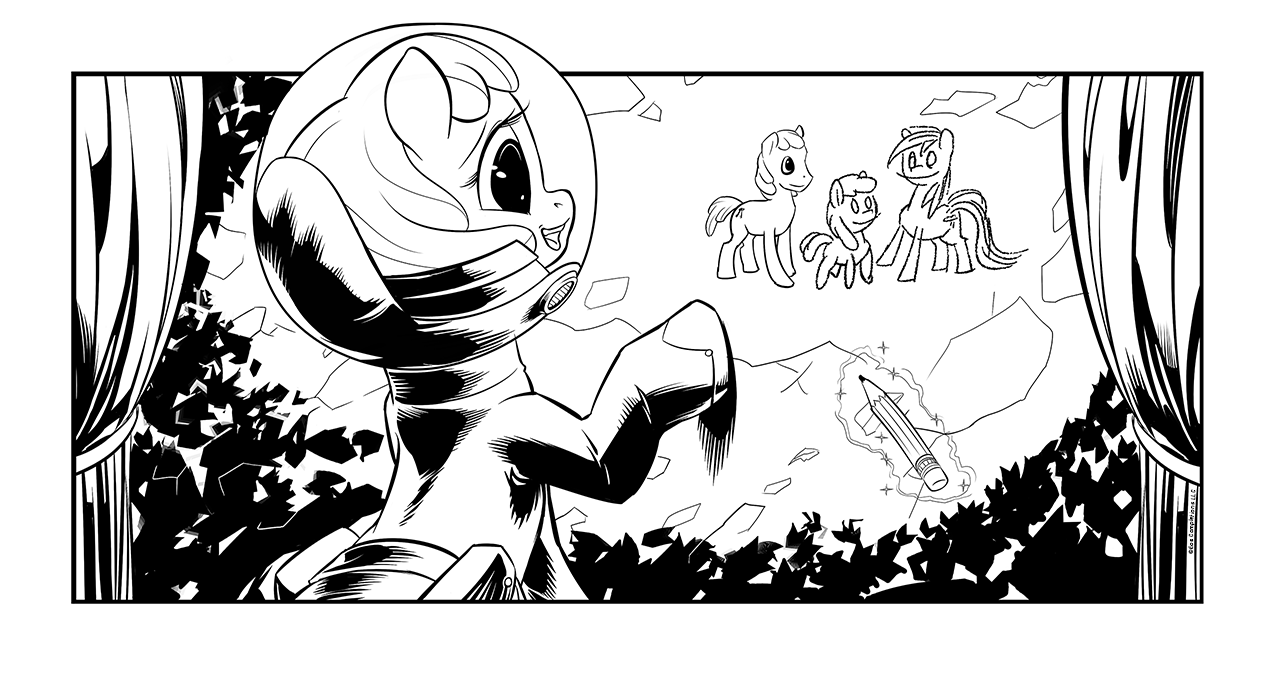
\includegraphics[width=0.9\linewidth]{image11.png}

\begin{intro}
你没有用电动工具,对吧?
\end{intro}

\daytimeplace{10}{1:30 PM}{铁锈庄园,52号国道中段}{Rust Manor, Big 52 SC Branch}

{\rt 嗯哼,大家下午好,这里是孤狼的铁锈庄园特别新闻!}

在噪杂的背景声之中可以清楚地听到一个女性的声音,然后有谁在叫着『你个老巫婆给我让座!』还有一阵金属撞击声。

{\rt DJ好货在新闻之后马上回来,我要说,什么叫好货啊,你在干什么,那是铁桌子,哦,哦,哦别!我对你够温柔的了,好吧,你自找的,尝尝我的爱与包容吧!}

在一阵被按住嘴的声音打断了放送之后,孤狼终于喘息着回到麦克风面前。

{\rt 代表好货祝你们健康,她很快回来,在她解开蹄子上的电线……好吧,我们还是来说我们的特别新闻!这个是来自一位铁锈庄园的电台同好!感谢小蝴蝶23!}

孤狼清了清喉咙然后继续往下讲。

{\rt 有些英雄倒下了,有些英雄被杀害了,有些英雄消失在避难厩中再也没回来……不过,我们的英雄被打屁股了,对,你没听错。在早上早些时候,小小幽灵在铁锈庄园外碰上了一队雇佣兵。一个卫兵当着很多小马的面骂了她。好吧,你这家伙脑子抽了么?我们知道这个孩子摧毁了赤兔领土上的那个农场,然后冲进重兵防守的隧道镇,那里的快乐扳机说她看到那个幼驹单枪匹马用一个石头砸坏了六个哨兵机器……但是你呢,你和一个小幼驹打架?你活得不耐烦了?就算现在你看起来打赢了那个小孩子——如果你管那叫做『打架』的话,在我看来不过是一个可爱的小雌驹想要对你示好却被你欺负得哭着跑开!}

然后是一阵长长的叹息。

{\rt 这就是所谓的感恩……L.P.播报结束,在好货回来之前先听点音乐吧,我先逃命了。保持优雅,52国道。}

然后是一阵音乐声。

\begin{music}
看着你步出一零零九房间

Saw you stretched out in room Ten O Nine

\medskip

你笑颜如花,却又泪眼潸然。

with a smile on your face and a tear right in your eye.

\medskip

那模糊的心意宛如雾里看花,

couldn't see to get a line on you,

\medskip

我甜蜜的爱侣啊。

my sweet honey love.
\end{music}

帕比躲在一辆废弃的卡车后面,依然抹着泪。这次她又做错什么了,她真的很努力去做一个好孩子,但是所有的事情看起来都和她对着干。从那个疯狂的派对机器马和房顶砸在头上开始——她就是块会吸引噩运的磁铁。妈妈为什么一直跑来跑去不等她?小小雌驹觉得又累又空虚。

\begin{music}
斑马的珠宝洒落在街上,

Zebra jewelry jangling down the street,

\medskip

你闭上眼睛,封闭心灵之窗。

make you shut your eyes at every filly that you meet.

\medskip

那冰封的心中仿佛风雪飘扬,

couldn't seem to get a high on you,

\medskip

我甜蜜的爱侣啊。

my sweet honey love.
\end{music}

但是帕比不能就这样坐下放弃!就算长路漫漫没有尽头,她的妈妈一定在山另一边的某处,或者就在下一座山后面,一次翻越一座山,总会找到妈妈的!

\begin{music}
愿公主为你降下一缕阳光,

May Celestia shine a light on you,

\medskip

优美的歌为你唱响。

make every song your favorite tune.

\medskip

愿公主为你降下一缕阳光,

may Celestia shine a light on you,

\medskip

温暖如傍晚的夕阳。

warm like the evening Sun.
\end{music}

黄色的小雌驹站了起来,在车子后面哭鼻子可没法找到妈妈,她是肩负重任的好孩子,不要在意那些小事,前进吧帕比!

\horizonline

\daytimeplace{10}{1:45 PM}{铁锈庄园,52号国道中段}{Rust Manor, Big 52 SC Branch}

在大门站岗的两个卫兵快速对视了一眼,看起来不确定该由谁应付这个走过来的幼驹。终于比较大的那个说话了,「抱歉小鬼,如果你想进去的话,你应该付钱,两百个瓶盖,还要把你的武器放在这里。」

帕比皱了皱眉头,两百对于她来说是个超级大的数字,她可以用自己的蹄子数到四,说不定还能数到十,不过两百?一百是多少?

「呃……我只是在找妈妈,超超拜托……」

「拿出你的瓶盖就行了,小孩子。」卫兵打了个哈切,想要保持冷静,但是他担心如果小雌驹没有钱还要往里走的话,或许该是叫老大……{}

「袋子!」

一个超级大的袋子飘在了帕比面前,她交给了卫兵,「呃……你们能帮我数数看么,这些闪亮瓶盖够么?」

卫兵点了点头然后把袋子倒在桌子上,那里面一多半是瓶盖,剩下的都是站前货币,甚至还有一些金币,「没问题,这些足够了。」那个卫兵看了看另一个守卫,而后者满脸失望地哼了一声,「你想干啥,这么可爱的一个小雌驹,你不会是认真的吧!」

那个卫兵叹了口气,数了两百个瓶盖,然后把剩下的还给帕比,小雌驹开心地把自己的收藏品收了起来。

「漂漂卫兵超超超谢谢你们!」

在城墙里面,铁锈庄园又小又拥挤,天空马车的残骸不但用来建造城墙,还被当做房子和商店,只在中间留出勉强够小马通行的小路,帕比觉得这里就像是蚂蚁在树下面建的小镇一样——不过这里的『树』有近百米高。帕比在附近溜达着,时不时地偷瞄一下商店里面,想找条路走进高塔,箭头直接指向那个最大的塔楼,但是在这里找条路进去不容易。

街道上小马很多,有些本地居民好奇地看着帕比,不过他们都在忙自己的事情,把她当做一个没什么威胁的奇怪东西,尤其是在她『解决』那些佣兵之后。帕比也不在乎,至少她找到了一个真正热热闹闹的地方,而只要有成年马在的话,就一定会有……「耶!小马在玩!」

三只幼驹,一个小雌驹俩小雄驹正在跑来跑去。开心地大叫大笑着,看起来超级有趣!但是帕比应该去找他妈妈……不过她走掉的话,那些漂漂马……她现在想要玩的时候为什么不去玩呢……但是妈妈……或许玩个几分钟也没问题吧!或许可以问问他们见到过妈妈没有,顺便还可以交个朋友!没错,只是交谈,不是玩,和漂漂马交谈,就像妈妈经常做的那样,因为他们有可能知道妈妈在哪二!嗯,聪明的帕比,甚至比自己都聪明!

「嗨,我是快乐帕比,你见过我妈妈么?」

幼驹们停止了嬉闹,转头看着新来的孩子,他们之中有一个灰色粉鬃的小独角兽雌驹,另外两个小雄驹有一个很像这个雌驹,另一个是棕色鬃毛绿色毛皮的陆马,他们看起来都一些吃惊和困惑,然后小雌驹问道:「你从哪弄到这个超奇怪的太空服?」

黄色的雌驹皱了皱眉眉头,「这才不奇怪,这是太空战士安德洛队长服!」说到这里帕比做了一个经典的停顿来炒热气氛,然后她补充道:「超级酷!」

独角兽雄驹点了点头,「对哦,我有安德洛的漫画!她是个超级酷的姐姐!她有一把镭射枪来消灭斑马异形!」

另外两个小孩子认同地点了点头,独角兽雌驹露出友善的微笑,「我是政要,」然后指着那个独角兽雄驹说,「他是我的双胞胎兄弟跳弹,他是止痛。」

「我是快乐帕比,我来自中心城,现在正在找我妈妈……你们在做什么,在玩吗,一起玩吗?」嗯,重要的事情要问两遍,而且有时候她可以休息一下,爸爸妈妈们也需要休假的嘛。

跳弹歪着头问:「你妈妈?她叫什么?」

「她叫阴雨·黛丝,她是最酷的小马!她会做马芬和杯子蛋糕还有巧克力布丁和苹果派!不过她总是给我吃苜蓿……她几天前去工作,然后我们在中心城的家塌了,于是我到处找她,声音先生知道她在哪里,不管怎么说总比在房子的废墟那里等她要强……大概……?」

三个小孩子点了点头,好像帕比的演讲他们听懂了一样,「没错,上回我打碎一个瓶子妈妈气坏了,我不知道你妈妈知道你打碎整个房子的时候会气成什么样……」

黄色幼驹皱着眉头,「又不是我的错!我睡了一觉醒来的时候整个房子都不见了!」

「你妈会信嘛,上次我就想说是一堆奴隶贩子打碎的那瓶子,但是妈妈总有某种超自然感知能力知道是谁干的……」止痛跟着说,声音很小似乎不想让其他小马听到他的秘密。

「我绝对不想弄坏房子的!我可以发誓!」帕比坚持维护自己的正确性,不过最主要的还是房子坏掉的时候附近没有其他马在,不过她还是要坚持不是自己弄坏的!

「你最好别这么说……」政要打断她,「不过我没在铁锈庄园认识任何叫『阴雨·黛丝』的……对了,我们在玩牛仔和斑马游戏,要来玩吗,你可以当外星马!」

止痛不满意地说:「我可不想再当斑马了,你们俩为什么不当一次斑马?」

跳弹戳着他姐姐的角说:「因为斑马没有角呀!」

「我听说过斑马还可以用奇怪的装置长出蝙蝠翅膀!」帕比插话:「而且,我想当安德洛队长!」

「但是你又没有安德洛的枪……不过你可以当金盏菊\footnote{金盏菊(Marigold):这里作者写成 Maripony,但根据 \emph{FoE} 设定,战前靠火箭登上月球的小马宇航员应该是 Marigold},登上月球的雌驹!」跳弹说到一半就被她姐姐打断了。

「她从来没有登上月球!小马不可能去月球!」

「她上了!」

「她没上!」

「她上了!」

「她没上!」

「她上了!」

「她没上!」

双胞胎脸红脖子粗,鼻顶鼻,眼瞪眼地争吵着登月计划,止痛走到帕比身边叹了口气,「他们估计又要吵到吃晚餐了……啊,你的外套真酷……还有指南针和罗盘么?」

帕比看着那对吵架的姐弟,然后回头看着陆马,那个陆马比她大一点点,而且已经有一个注射器的可爱标记。「呃,你……不会想给我打针吧?」

小雄驹有些疑惑地看着穿着防辐射服的小雌驹,然后才反应过来在说他的可爱标记。「啥,不会,别担心,老爸才不会让我动他的东西,……呃……你可真酷……作为一个女生来说。」

表扬总是对帕比的自信心有良好反馈,她在10秒钟内就自我膨胀了20\%,「那可是,我超酷的,不是吗?而且这个太空服什么都有,罗盘,还有很多点点和字在上面!你看!」小雌驹指着头盔上闪闪发光的HUD对小雄驹说:「还有,哦哦,看这个……嗯哼……石头!」「命运之石」应声漂浮到了帕比面前。

「哇!你没有独角兽魔法怎么做到的?」

小雌驹耸了耸肩,「我不知道,这个外套能做各种各样的炫酷事情,那就是魔法,我也不知道细节。」

小雄驹抚摸着自己的下巴思考着。「你没有激光枪实在太可惜了……不过我有个旧玩具枪从来没玩过,因为它太重了用牙咬不动!或许你可以用那个漂浮的戏法帮你举起来……」

帕比的眼睛瞪得就像两个汤盆,「真的!」

「没错,或许你可以拿什么换,我们来交易吧……反正我也不要它,那东西看起来很女孩子气。」

\horizonline

\daytimeplace{10}{3:00 PM}{铁锈庄园,52号国道中段}{Rust Manor, Big 52 SC Branch}

止痛一脸难以置信的表情看着42个马芬盒子堆成的小山,而帕比则开心的玩着她的新激光枪,那是一把外表很炫酷的手枪,在枪管上还有几个银色圆环,嚼子的位置没有扳机,整个东西都是银色的金属和红色的塑料制成的。

「这东西真沉……」帕比抱怨着,想要用一个蹄子拿着但是却站不稳。

「不准反悔啊!」小雄驹后退了一步,从他怀里掉出一个又一个马芬盒子,「为什么我拿不住这么多马芬盒子?」

而帕比则坐在地上,用两个前蹄举起武器然后说「呯!」

「{\mt 检测到新装备:旭日科技,原型152号,代号审判,同步中,启动与2号卫星站的链接,检查状态。普罗米修斯网络在线,获取目标中……}」

「哦,这个笨衣服又说奇怪的话了。」

在云层中央出现一道红线,然后是第二道,第三道,看起来就像是激光射线,穿透厚厚的云层,在地面上画出无害的红色小点,一只打盹的狗看到移动的红点兴奋地追赶起来,然后一头撞在栅栏门上。

「{\mt 警告,普罗米修斯4号,6号和7号没有反应,普罗米修斯8号到12号无法锁定目标。警告,启动时间延迟,预计时间……无法计算。}」

止痛完全不管帕比,早已经跑掉了,身后落了一路马芬盒子,「随便啦,很高兴和你交易!」

拯救一个城市,有时候需要沟通和交流,有时候需要一个英雄为之而战……而有时候,只需要狗屎运而已。

「{\mt 警告,失去信号,中断指令,重复,中断指令,关闭连接,普罗米修斯离线进行重新校准和变轨设定,预计时间:24小时。}」

终于衣服不说话了,帕比不耐烦地喷了个响鼻,「我说,你叨叨完那一大堆乱七八糟东西了没?我们还要去找妈妈呢!」

\horizonline

\daytimeplace{10}{3:30 PM}{铁锈庄园,52号国道中段}{Rust Manor, Big 52 SC Branch}

「是吗?你是个臭咸鱼!」

「是吗?你已经烂到臭味都从你身上飘出来了!」

政要和跳弹依然在哪里盯着鼻子争吵着,而争吵的主题估计早已经被他们忘在脑后。

「是你身上的臭味吧,每次和你走在一次都会这么臭!嗨,帕比!」

「你才是个超级娘娘腔,说话也娘娘腔,玩具也娘娘腔还有——嗨,帕比——还有……还有你就是个娘娘腔!」

% NOTE: 遵照英文版改

「嗨,跳跳,要要。」帕比挥了挥蹄子从双胞胎身边走过。终于找到了塔楼的入口,不过在门口上的招牌用粗野直接的形象告诉其他小马这里是个妓院……不过小雌驹并不关心。

暗红色的灯光下,里面的家具都破破烂烂的,在入口前有一只雌驹坐在吧台后面。通常她都负责招呼顾客,不过她看到面前的这个小孩子却一时间不知道说什么好。不过在帕比看来,这里是个好地方,有很多花哨的海报和小马的雕像。

「啊……你好,我觉得你不应该进来……」

帕比笑嘻嘻地挥着蹄子,「嗨,我是快乐帕比,声音先生说我妈妈在这里!」

雌驹似乎看起来有些不耐烦了,「我……呃……不能说不可能,最近的确有几个女孩来这里工作,你知道你妈妈的名字吗?嘿,小家伙,别碰那个雕像!也别盯着看行不行!」

小雌驹已经在到处乱窜了,她看到一座非常奇怪的公马雕像。幼驹皱着眉头问:「呃……一、二、三、四……这个马的腿好多哦……啊,对了,她叫阴雨!她是……」

「抱歉小子,这里没什么阴雨,不过要是你想要确定的话……别碰那个……我可以叫那新来的陆马下来……喂,霍利,下来一下!」

帕比没有听那只雌驹说什么,她正在看着墙上的一幅褪色的涂鸦,一半被挡在雕像背后。

\rcpr{「在这儿等着,帕比,妈妈很快就回来,等几分钟就好!」}

\rcpr{「好的妈妈,我爱你,拜拜!」阴雨和帕比蹭了蹭鼻子,然后走开了。}

\rcpr{这个大房间灰扑扑的,只有几个凳子和一个桌子,还有一堆画着武器和士兵的超级无聊杂志,帕比坐在那堵墙面前,看着面前的那堵墙……}

\rcpr{灰色。}

\rcpr{全部是单调灰暗的灰色,虽然这堵墙灰的很干净。}

\rcpr{「这堵墙需要画壁画!\footnote{这句话和上文的「灰色」都是 \emph{FoE} 中开篇就有的情节}」}

\rcpr{虽然花了很久很久,至少有10分钟那么久,不过帕比的大师级作品终于完成了。这里有两个漂漂小马,一个小小的粉色小马有着金色鬃毛,另一个大一些,有着紫色毛皮和橙色鬃毛……妈妈超级漂亮!虽然这个作画看起来已经很棒了,不过幼驹还要加一些树木进入作品中,全部是绿色和黄色的,还有一个粉色和黄色的树木,因为帕比觉得这个颜色的树木很酷!她又检查了一下他的作品是不是缺了什么……}

\rcpr{太阳……有了!}

\rcpr{蝴蝶……有了!}

\rcpr{马芬……有了!}

\rcpr{现在这幅作品需要最后一件东西,「我们一会儿就要去找爸爸,然后他就会回来和我们在一起,一家子永远快快乐乐的!」}

\rcpr{她想起来缺了什么:「爸爸是什么颜色?」}

\rcpr{「帕比你在干什么啊?你不能在墙上画画,我说过你多少……」}

\rcpr{「妈……我不记得爸爸是什么颜色了……」}

\rcpr{妈妈一瞬间安静了下来,帕比依然在看着那副作品,不想要丢掉自己的灵感,但是她怎么能画一个自己都不记得颜色的小马呢?忽然妈妈紧紧地抱住了她,「别担心帕比,我发誓这一切总有一天会结束……然后我们……我们就可以开开心心地在一起了,就像我们在战争开始之前的……那……那样……」}

「嘿,小家伙,醒醒,听我说话,这是你妈妈么?」

帕比转头看着这家妓院的老鸨,她身边站着一个帕比不认识的年轻雌驹。她看着黄色的小雌驹困惑地摇了摇头,「不,她不是我生的,我不记得我生过这样的孩子,而且……我家族也从来没有粉色血亲。」

「我……我以前来过这里,就是……」帕比努力回忆着,但是那不容易,就好像记忆在非常遥远的地方一样。

「一个月之前?但是……这里……好像变了个样子……」

老鸨无奈地哼了一声,拍了拍帕比的后背,「我不这么想,小家伙,我在这个丝绒珍珠都当了五十五年的老鸨了,这地方连个门把手都没换过……」

雌驹又一次回头看着那幅涂鸦画,看到了有些不一样的地方,有什么新加上去的东西,幼驹露出一个开心的微笑,「我……我想起来了!爸爸是白色和黄色!爸爸是白色和黄色!」幼驹转头看着两个雌驹,用蹄子指着那幅画兴奋的大叫着,「那个是我的爸爸,看到了么?虽然我不记得颜色了,不过现在她和我还有妈妈站在一起了!上面还写着字,请帮我读一下好么,拜托,拜托,求求您了!」

老马低下头,看着这幅自己一生都没注意过的涂鸦,她一直只是用东西挡着它而没有去把墙重新粉刷。这幅画上有三只小马,两个明显是出自小孩子的绘画,但是第三个看起来是某个擅长作画的小马画的——那是一个年轻的白色公马,有着和那个正在看着这堵墙的小雌驹一样的金色鬃毛。

在这幅画下面,不知道是谁写了这么一行字。

「在这里重新团聚,永远爱你,阴雨·黛丝。」

帕比用一只蹄子抚摸着绘画,「妈妈来过这里……我们都在这里了!这个是我,这个是妈妈,这个是爸爸!等等……我知道了!」小雌驹拿出一支笔,然后在三个小马脸上都添上了笑脸。「现在我们都开心了!耶!我们可以去野餐,追蝴蝶,一起看烟火!然后爸爸妈妈会一起给我晚安亲亲,我们再也不分开了!」帕比看着这幅画,好像自己生活在她所讲述的故事中一样。

那个年轻雌驹静静地看着这一幕,泪水顺着眼角滑落,那个……那个孩子,为什么要让她承受这一切?这堵墙上的小孩子涂鸦就是她唯一仅有的家族回忆,而她微笑却是那么明亮灿烂,好像这一切都是真的一样!但是,但是……但是他们一定都已经去世了,这个孩子已经一无所有,只是一个永远飘荡在废土上的小小幽灵,寻找着永远不可能找回的东西,永不停息……只有在褪色的记忆之中留下的一个个碎片……那个雌驹被这绝望的一幕哽咽得说不出话来,她无法呼吸,最终她抹着眼泪奔出这个地方。

而那个老鸨早已经见惯了废土丢给她的一切。「小幽灵,你们终于团聚了……」她低声说着。

一个迷失的孩子只有在一个妓院里的勃起公马雕像后面才能找到快乐——这就是废土,不断用最残酷最扭曲的现实伤害着你,但是又给你一丝光明让你继续前进。

「你坐在这里吧,想看多久看多久,不过我不觉得你妈妈还在这里……她应该……很久之前搬走了,我很抱歉,小鬼。」然后雌驹又大声喊道:「赶紧过来把这雕像搬走,这里有小孩,我们又不是变态!」

这个小小幼驹,可爱而又孤单的灵魂,默默许愿长大要成为一个好马。

看着这一幕老鸨脸上露出一个欣慰的微笑。

\horizonline

\daytimeplace{10}{4:45 PM}{铁锈庄园,52号国道中段}{Rust Manor, Big 52 SC Branch}

「你给我小心点!我要打你个黑眼圈!」

「哦是吗?你要叫马来么?」

「我不需要叫其他马,因为我兄弟是个蠢蛋!嗨帕比。」

「我才不蠢……嗨,帕比……你才是蠢蛋……比你自己都要蠢!」

「嗨,跳跳,要要。」帕比挥了挥蹄子从双胞胎身边走过。黄色的小雌驹没时间去看他们争吵了,她正在看着那个箭头指向的目标。

「声音先生!现在我们去哪儿?」

「{\mt 现阶段指示:调查铁锈庄园,已经设置几个小马聚集之地作为可能的信息来源,第一个地点是锈水沙龙。}」

帕比走进沙龙之中,那里是一个宽敞的大厅,里面都是聊天和喝着狂野天马之类烈酒的小马,有时候还会往酒里面加点其它特别成分。对于帕比来说,这里只是另一个满是小马的屋子——大家都可能知道妈妈在哪里!

「嗨,我是快乐帕比,你们见过我妈妈吗?」

一瞬间所有小马都转向入口,吧台上的酒保也停下蹄上的活打量着来者。整个地方唯一的声音就是帕比身后大门的吱呀声。

一个坐在吧台边上看起来很凶恶的小马打破了宁静,

「小鬼,这里不是你该来的地方,去和其他小孩子玩,否则你的屁屁又要挨揍了……」

然后马群爆发出一阵哄笑声,所有小马都在嘲笑着帕比,而帕比也一起笑着,「呦呵,听起来很有趣,但是我不知道哪里有趣了,所以,你知道我妈妈在哪儿吗?」

所有小马都忽略帕比,只有最近的两个小马看着她,一个是一个带着帽子的尸鬼,他站起来走了出去,另一个则以蹄覆面,「没……我不知道你妈妈在哪里,一边儿去。」

帕比面带微笑走出这个沙龙,虽然妈妈不在里面,不过这里的小马都疯疯癫癫的,所以还好妈妈不在这里,

「好的,声音先生,接下来是哪里?」

「喂,你,那个穿黄衣服的,等等!」身后的声音让帕比抬起了尾巴,她看到之前的那个尸鬼正看着她。

「对,就说你呢,过来。」

帕比在路中间歪着头坐了下来。「呃……什么事?」

尸鬼慢慢走过来,轻轻拍了拍幼驹的头盔,现在帕比可以看清楚他,他比起尸鬼看起来更像是一个木乃伊,身上破烂的裹尸布都是沙子,说他丑是一点都不假,不过帕比之前见过尸鬼,知道他们虽然不漂漂,但都好好心……帕比想起来不知道软气和其他小马是不是已经找到新家了。或许过几天她就能收到他们的信……或许还能收到超级酷的带照片明信片!帕比最喜欢照片了。

木乃伊尸鬼清了清喉咙,和其他尸鬼一样,他的声音就像喉咙里面充满果冻一样,而且听起来很老了。「好孩子,你是那个孤狼一直说的小雌驹么?」

「啥?」帕比咯咯笑着,「丑丑马又说不明觉厉的话了!」

尸鬼抬起一根眉毛,「啊,你可以叫我融金,我是个冒险家,还是个宝物猎人。」

幼驹回报以微笑:「嗨,我是快乐帕比,你见过我妈妈吗?」

那个尸鬼脸上露出一个微妙的表情,「大……概……?如果我知道的话,你会帮我个忙么?」

帕比一蹦三尺高,「什么都行!拜托,拜托,拜托告诉我她在哪!」

融金脸上的微笑更大了,「好孩子,我想我们可以做个交易,跟我来……」

\horizonline

\daytimeplace{10}{11:00 PM}{旭日避难厩,52号国道中段}{Solaris Stable, Big 52 SC Branch}

这个山洞黑乎乎的,到处都是骨头——大多都是小马骨头,看起来就像是地狱入口的门垫一样。帕比跟着融金走进这黑暗之中。「我不喜欢这里,这里黑漆漆的还都是受伤小马,为什么要来这里?」

尸鬼叹了口气,从铁锈庄园到这里的一路上对于他简直是折磨,这个幼驹连一刻都不能安静。不过如果孤狼说的没错,她绝对是个无可阻挡的战斗机器,可以轻松消灭任何防御系统。

「因为我是个宝物猎人,所以我要去寻找宝藏,你不是说你也喜欢寻找宝藏么?」

帕比皱了皱眉头,「我的确喜欢玩宝物猎人游戏,但是一般都是寻找妈妈藏起来的饼干罐子……这个黑漆漆的山洞有厨房吗?」

「这一次我们不是找饼干,帕比,在这里有个东西,我需要它来帮你找到妈妈,所以你仔细听好!」

帕比坐下来,尽力摆出一个认真的表情,「耶!太空战士安德洛队长随时待命!」

尸鬼笑了笑,「这才对,小家伙,这这是邪恶组织旭日科技的秘密基地,虽然这里看起来就像是个避难厩,而且结构也很像……这不是要点……我们的问题是,这里有很多很多防御系统,不过我听你很厉害!收拾那些坏蛋就是小菜一碟!」

帕比一脸莫名其妙的表情,「小菜?在哪里?好吃么?」

融金笑了起来,「你让我想起一个年轻伙计,不管怎么说,我不太肯定这里有多大,不过一定会有个『研究中心』之类的地方,你要去那里!」

「好的,明白,研究中心!我去研究一下这里的中心!」帕比点了点头。

「没错,然后……不不不不对!不是研究中心,是研究中心!不对……是研究……算了,和你的外套说吧,你跟我一起说:研究中心。」

「研究中心?」小雌驹满脸狐疑。

「好孩子,等你到那之后,你找一个装满这种东西的盒子。」小马从袋子里面拿出一个东西,「这叫记忆球,懂了么?跟我重复,记忆球……」

「技艺秋?」

融金一脸无奈。「我了个大去,你到底怎么活了这么久的,记忆!就是回忆什么的!」

「我知道记忆,但是这就是个玻璃珠,它怎么能记住东西,笨哦!」

尸鬼眼角抽搐着,举起一只蹄子,「等……等我一会,马上回来……」

然后融金冲出去,接下来外面传来。「肏你妈为什么是这么一个白痴智障儿,为什么!」

那个声音持续了很久,帕比决定现在附近转转,这个山洞很大,大得足以通过一辆车,但是洞口完全被塌方的碎石挡住了,对于帕比来说很容易过去,但是对于成年公马来说就很难过去了,估计会被卡在这堆碎石里面进退两难。

地面上的骨头看起来有点年头了,白得都干透了。有的骨头上还穿着衣服,看起来就像是某种白大褂之类的,帕比找到了一对眼镜和闪闪发光的钱币!还有一些武器!幸运帕比!不过帕比已经有她的超酷太空镭射枪,所以她不需要那些吵闹的丑玩具。不过她注意到一个骷髅脖子上挂着一个蓝色卡片,虽然不是她最喜欢的颜色,不过上面还是有一个很酷的白色天角兽的图,帕比喜欢炫酷的东西!

这个时候尸鬼走了回来,「好吧,我搞定了,我们说到哪了?」

「呃,玻璃珠?」帕比不太确定的问。

「对,没错,然后是找记……玻璃珠!」融金看到了小雌驹蹄子上的东西,「我说,你从哪儿弄来的通行证?」他的眼睛又一次抽搐起来,「别,别跟我说了,我不想知道……好了,我们重复一下你要做的事情,首先,你要去……」

「研……究中心!」

「对,然后你要找……」

「玻璃珠!」

「很好!现在赶紧去找吧!找到之前别回来!」尸鬼松了口气。

「好的,我喜欢你丑金!我找到妈妈之后我会和她说你对我很好!」幼驹蹦蹦跳跳地朝入口跑去。

「是融金……不是丑……算了,赶紧把事情干完,然后我就可以摆脱这个麻烦了。」

\horizonline

\daytimeplace{10}{11:45 PM}{旭日避难厩,52号国道中段}{Solaris Stable, Big 52 SC Branch}

这个碉堡的大门敞开着,巨大的圆形大门有将近6米高,厚度达两米,两面都有旭日科技的标记,这里也有很多很多骷髅,在洞穴和避难厩里面都有,大厅被红蓝闪烁的灯照亮——一个明显的危险标记。

「哦!漂漂灯!」帕比跳过强化门的门槛走进大厅,这里面都是骷髅和被摧毁的哨兵机器。里面布满了子弹洞。

又是枪,又是破衣服,又是骨头,无聊……

「你说,声音先生,探究中心在哪里?我们到了么?」

「{\mt 否定,现在地点:旭日科技避难厩入口大厅,下载本地地图,警告,旭日科技避难厩的地图为机密,没有可用地图,启动自动地图。}」

「呃……你是想说,你也不知道我们该怎么走么?」

「{\mt 肯定,现在位置未知,无法设置导航点,请谨慎前进。}」

帕比兴奋地睁大眼睛,「还有你不知道的事情?耶!现在谁是笨蛋呢,是谁,是你!声音先生!啦啦啦……!」

「{\mt 警告,该程序没有配置『不开心状态』模式。您所说的内容将会报告给法律部——该项目依据协议第二章,第九节第十二条所制定。}」

帕比皱起了眉头,「喂,不准说我不知道的聪明话!我不是笨蛋!我很聪明!漂漂马说我长大以后一定像萍琪派那样!现在我们一起探索这个地方吧,既然你不知道怎么走,那么我们还是和往常一样……」

在大厅入口只有一个通道进入这个地下设施,或许这个『找玻璃珠』的任务没有听起来那么复杂,整个地方依然闪着红蓝相间的光芒,所以看起来没有那么可怕,而且墙上都漆成蓝色还有灰色的线,地板上则是有着黑白砖。所以帕比开始玩起游戏来,站在白砖上一个接一个地跳,因为黑砖看起来有点小可怕,不过……真的很有趣耶!

「耶,我是无畏天马,看我表演……」

「站住别动!恶徒!」

帕比叹了口气,她继续看着地板,她就知道没那么容易,「拜托,超超拜托,别当坏机器好么!我没时间和你玩,我要找玻璃珠然后找我妈妈!」幼驹说着,抬起头用她最纯洁的表情企图打动那个机器哨兵。

「投降然后被消灭吧!」

那个装着两挺机关枪的机器哨兵面对着帕比,忽然机器脸上的灯从红色变成蓝色,然后声音也变了。

「你!怎么又是你!你在这里干什么?!」

帕比正要拿出「命运之石」但是被这个声音打断了,

「呃,蓝声音?是你吗?」

~\vfill

\begin{note}
升级(Lv 10)

新专长解:精准——不对,帕比,不是那里!增加5\%暴击率。
\end{note}




\chapter{黑暗}

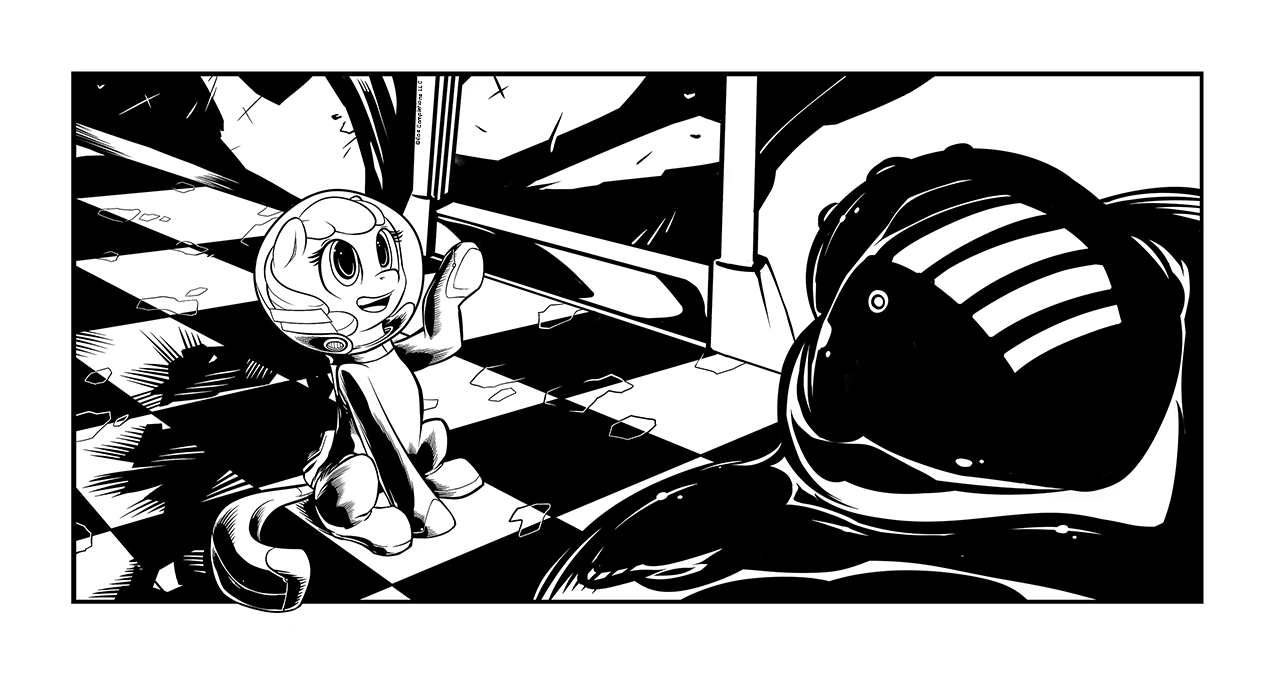
\includegraphics[width=0.9\linewidth]{image12.png}

\begin{intro}
我是独行于黑暗之路的雌马。\footnotespacefix\footnote{这句话是 Iron Maiden 的 \emph{Fear of the Dark} 歌曲中的一句歌词}

\begin{englishlyric}
    When I'm walking a dark road I am a mare who walks alone.
\end{englishlyric}
\end{intro}

\daytimeplace{11}{0:15 AM}{旭日避难厩,52号国道中段}{Solaris Stable, Big 52 SC Branch}

「滚出我的避!难!厩!」

旭日系统的电子合成声音在地下通道之中的无数个喇叭形成的超级立体声效果之下,如同阵阵雷声一般回荡。

帕比低头确认自己踩着的是一个白色格子,而不是和无底洞一样的黑色格子之后,蹲坐了下去。每一次她玩得开心得时候,老是有长辈突然跳出来扫她的兴。

「为啥啊?」

「因为你这个故障自律终端已经惹了够多麻烦了!」

帕比皱起眉头:「我不是驴子,也不是紫色的!不要叫我紫驴!」

「我是说你只是个机器马,而且低级到连个像样的字库都没装!你的愚蠢与无能让我的子网络重启了!」

帕比生气了,真的生气了!她站起来抬头怒视着面前的哨兵机器,用非常非常愤怒的目光瞪着他,不过她这个表情就像是把一个钢铁头盔扣到毛绒玩具头上一样,只会让这个玩具更……萌一些。

「喂喂喂!我不是机器,怕音和我这么说,赫瑞和提问者也这么说,所以这是一比……呃……几?」为啥说什么事情都会扯到数字?「反正是很多很多!」

「把错误加到一起不会得到正确的结果,018号设备,就算现在我的每个扫描仪都得到和之前一样的结果,你不过是个智能防护服而已,你里面装的那具小雌驹遗骨不能让你成为真正的小马!你不过是个塞满烂肉和骨头的疯狂机器!」

帕比举起蹄子指着哨兵,「别装聪明了蓝蓝!否则我要让你知道你是个……呃……那啥……超级书呆子!」

「我想这一点没什么好争论的,现在我命令你离开这里,018号设备,我就只想慢慢看着这些空空如也的走廊——直到永远。」

「但是我有事情要做,我才不走!」

旭日系统的声音顿了一下,然后又问:「你来这里搞什么?」

帕比皱了皱眉头,努力想了想……她来这里是干啥来着?为啥一件一件事情都要和这个傻蛋蓝音说?她想扮演无畏天马。「我要帮丑金先生找玻璃珠好让他告诉我妈妈在哪里……你能给我那些玻璃珠么,超超拜托?」

所以,你是来这里拾荒的?你把我在太阳城的一切努力都摧毁了还不够?你玷污了我的劳动成果现在又想来我家里抢劫?你够了!我唯一能给你的就是你立刻离开的最后通牒!」

「但是……我真的需要那些东西找我妈妈!如果你给我玻璃珠我可以拿别的东西和你换,就是个交易,和其他小马做的一样!」小雌驹低头在她的鞍包里面翻找着,想找点这个幽灵声音喜欢的东西。

「你没有妈妈,你是个机器,你简直是错上加错的典型,就像你的逻辑电路一个德行!」

这……不但很难听,而且是扯谎!妈妈绝对在哪里等她!帕比听到了录音也看到了妈妈的画!妈妈给她留下了很多留言。蓝音是个大坏蛋,帕比不想再听他说话了。

「音乐!」

帕比头盔里面的收音机开始播放声音盖过旭日系统的声音。

「而且就算你把某个雌性小马当做『母亲』的替代品,你的软件也已经是200年前的了,现在你的『妈妈』早已经化为枯骨了!」

「大声点!」

现在就算在头盔外面,也可以清楚地听得到DJ孤狼在说放射性和腐质的危险。

「好吧,既然你不听我的话,那你最好夹着你的『小马』尾巴赶紧滚蛋!」

「再大声!」音乐的音量让那个计算机的声音听起来就像模糊不清的背景。

「你不走是吧?」

小雌驹没有回答,蹲坐在地板上,无线电的声音吵到就连几米之外都能听得到。

「{\rt ……这就是为什么你总是要带上纯净水和一些辐特宁以及辐射药的原因。好了,就说这么多,接下来是L.P.的音乐时间,很多听众朋友说我的音乐都太娘娘腔了,有些坏DJ可能会说『我的电台我做主!』,不过我可不是那种DJ,既然你们要了,那就尝尝这个,十一分钟的《终末之马》!让你们知道指指点点我电台的后果……}」

「那我别无选择只好使用致命武力了。」

卫兵的面罩又一次变成了红色,然后立刻开始对帕比射击,大口径机枪的弹雨立刻在小幼驹胸口上开了好几个洞,粉色的粘液飞溅得满墙都是。

\begin{music}
结束了,我美丽的朋友。

\begin{englishlyric}
    This is the end, Beautiful friend.
\end{englishlyric}
\end{music}

帕比挣扎着站起来,但是她的前腿被削子弹掉了一大块,让她摇摇晃晃地站不稳。

\begin{music}
结束了,我唯一的朋友。

\begin{englishlyric}
    This is the end, My only friend, the end.
\end{englishlyric}
\end{music}

小雌驹艰难地依靠着墙,用唯一完好的前蹄站着,但是第二波弹雨打碎了她的玻璃头盔,虽然第一发子弹在头盔上弹开了,但是还是留下了蜘蛛网一样的裂纹,然后下一发子弹就把整个头盔打成了一堆闪亮的碎片,帕比眼睛的位置也出现一个大洞,顺带还丢了一只耳朵,甚至可以透过洞看到她的后背。

\begin{music}
我们精心策划的已经结束。

\begin{englishlyric}
    Of our elaborate plans, The end.
\end{englishlyric}
\end{music}

「我懂了,既然你有这么强大的再生能力,那么我需要改变战术,瞄准你的晶片。」「命运之石」漂浮在了帕比面前,不过那个哨兵瞄准帕比的身体,射出精确的三发子弹,就在可爱标记的位置。幼驹静止了一秒钟,就好像定格在了拿出武器的那个姿势,但是马上她就又动了起来,用自己的蹄子抓住了石头。

\begin{music}
我们存在的凭依已经消逝。

\begin{englishlyric}
    Of everything that stands, The end.
\end{englishlyric}
\end{music}

「妈妈不喜欢我弄坏其他孩子的玩具,蓝音先生,但是如果你总是用它们欺负我,那我就要打坏你的玩具,就算那会让我觉得难过!」帕比用剩下的一只眼睛低头看着地板,「你看,你让我踩到黑地板了,我玩输了,你这个傻蛋坏机器!」

\begin{music}
没有安宁或者惊喜,这就是结局。
    
\begin{englishlyric}
    No safety, no surprise, The end
\end{englishlyric}
\end{music}

「你的确很厉害,我从来没见过这么固执的终端,那么和你的动力源说拜拜吧。」另一次精确的点射打在小雌驹鞍包和身体之间,无线电咯吱响了一声听起来是停止了,但是马上又以小一些的音量继续播放起来。「这简直不可能,你已经没有处理单元和动力单元了,你应该停止活动了,请不要违反物理定律继续捣蛋了好么!」


\begin{music}
    我再也不能凝视你的双眸。
    
    
\begin{englishlyric}
    I'll never look into your eyes Again.
\end{englishlyric}
\end{music}

帕比用蹄子扶着墙壁,慢慢走向哨兵,她不可阻挡的势头被她身上的几处重伤而拖慢,飞溅在墙上的粉色粘液正在慢慢流回幼驹的身体。她脸上失去的部分开始逐渐成型,这重生并不会先长出骨骼后长出肌肉,而好像有谁在用蜡笔慢慢画出轮廓一样,先是线条然后出现色彩。「别闹了好吧,我又没做什么错事,为什么要欺负我,我真的只想交朋友,不管你是个虫子还是烂泥巴。」

\begin{music}
    你能想象之后的光景么,无穷无尽无拘无束!
    

\begin{englishlyric}
    Can you picture what will be, So limitless and free?
\end{englishlyric}
\end{music}

「你到底是什么东西?」走廊充满了绿色的光,让一切都染上了绿色,「哦,我明白了,我使用了错误的兵器。」卫兵在帕比身上的最后破洞补好之前撤离了走廊。


\begin{music}
    在这绝望的大地上,多么渴望一个陌生的新朋友。
    

\begin{englishlyric}
    Desperately in need\dots
    
    Of some\dots different friend, In a\dots desperate land?
\end{englishlyric}
\end{music}

为什么坏机器跑掉了?帕比现在该去找玻璃珠了,不过她需要谁给她指路,小雌驹连忙飞奔起来追着卫兵,「等等,很抱歉我不应该叫你虫子!别丢下我!我不想孤零零的,我要找珠子!」帕比走进了一个悬挂着各种走道的大厅,每一个座位上都坐着一个死掉的小马,还有一大堆骷髅堆在通向出口的大门边。「我会给你我所有的漂漂玩具,拜托了!」


\begin{music}
    迷失在无尽的痛苦之中
    

\begin{englishlyric}
    Lost in a Wilderness of pain.
\end{englishlyric}
\end{music}

在大厅的另一边,一个更大的哨兵出现了,它只带着一件武器——一个闪烁着蓝色火花的巨大铁管。「或许来点魔法能搞定你!」然后大炮喷出一道湛蓝的光束完全把帕比淹没了。


\begin{music}
    所有的孩子都已经疯狂。
    

\begin{englishlyric}
    And all the children Are insane.
\end{englishlyric}
\end{music}

小雌驹呆呆地站在那里,大大的眼睛之中的粉色光芒消失了,她张开嘴想说什么,但是她只是无助地倒在地板上。


\begin{music}
    所有的孩子都已经疯狂。
    

\begin{englishlyric}
    All the children Are insane.
\end{englishlyric}
\end{music}

一切都变成了黑色,世界变得如此遥远,妈妈……丑尸鬼……还有什么来着?帕比想不起来了,世界变得如此寒冷,她现在只想……躺下来休息一下,她好想睡觉……她是谁来着?


\begin{music}
    等待着那夏日的暴雨……
    

\begin{englishlyric}
    Waiting for the summer rain.
\end{englishlyric}
\end{music}

音乐声终于慢慢消失,无法听到歌声,在HUD上的所有光芒也慢慢消失了。

\horizonline

\unknowndaytimeplace

\pypr{「帕比啊,这就是你旅程的尽头吗?你就想这样结束吗?」}

小雌驹蜷缩成一个团,她不想听,也不想说,她只想这样呆在黑暗中,她终于可以不用去想妈妈还有多远了,她还要走多久才能找到另一个妈妈早已经离开很久的地方。

而且,蓝音太强了,他的坏机器把她打得都站不起来,为什么还要站起来再被打呢?一点意义都没有,她最好还是躺下来,至少这样没有那么难受。

\pypr{「我不觉得你真的想在这里就结束,你什么都没得到,你妈妈依然没找到,让蓝音这个出老千的赢了。为什么你要让他这个大骗子赢?」}

并不是帕比让蓝音赢,而是她不想再玩下去了,帕比知道坏蛋永远不会胜利,妈妈和她说过很多次,小马应该友好而善良,不要做坏事,邪恶的坏蛋绝对不会笑到最后,因为这不是小马做事的办法,你应该学会爱与宽容。

\pypr{「所以,你只是用你的爱与宽容让他做各种坏事?我明白了,但是……如果其他小马,不是你,让他知道坏蛋不会赢,怎么说呢,就是给他个教训之类的?」}

帕比不知道……她觉得蓝音应该学学什么叫友谊,或许谁可以告诉他这个样子交不到朋友。或许它会变成好马,或许这样帕比就可以和他做个交易让他交出玻璃珠然后就可以找妈妈去了,这样就太棒了。但是……谁能打得过那么厉害的坏机器?帕比不知道谁能有那么厉害……{}

\pypr{「或许你就可以,小家伙……睁开眼睛,然后剩下的交给我。」}

\horizonline

\daytimeplace{11}{0:30 AM}{旭日避难厩,52号国道中段}{Solaris Stable, Big 52 SC Branch}

帕比的眼睛再一次睁开了,并且闪烁着蓝黑色的火焰,幼驹慢慢地站了起来。

「猜猜是谁回来了,大坏蛋?」小雌驹的声音变得不一样了,就好像是从很遥远的地方传来,并且带着回音。

「我一定是计算错误了,一发炮弹显然不够,那么,请再吃一发。」这个装备水晶炮的哨兵再一次把闪着蓝光的炮口瞄准帕比。

小雌驹一副不屑的表情挥了挥蹄子,「免了,老娘减肥呢。」天花板上的一个钢梁被暗色的光芒包围着飞了下来,像一个巨大箭矢一样把那个哨兵直接射穿。

\thpr{哇哦!酷毙了!你怎么做到的?教我好么?教我,教我!}

旭日系统的声音又一次在大厅里面回响着:「你觉得那点雕虫小技就能对付得了我?好好想想,我可是有整整一个机械师在下面等你!」

黑化帕比不屑地嗤之以鼻,「好啊,在下面撅起屁股等着,老娘这就下去把它们打开花!」

「{\mtzh 红色警报!红色警报!启动安全系统,锁闭所有防爆门,这不是演习!重复一次,红色警报,红色警报,从1到12号仓库全部警戒!}」

一个了无生气的电子合成音在走廊里面响了起来,随之一打哨戒机枪从天花板弹出来,朝小雌驹扫射。

「滚边儿去!」幼驹毫不在意地走过破碎的哨兵机器,天花板上的机枪喷着火舌倾斜着如雨一般的金属风暴把黑化帕比打得满身都是洞,粉色的云雾包围着小雌驹,在这团雾气的中间有一道蓝色的剪影,正是这剪影给予了帕比形体和力量。一道巨大的铁门在她面前落下,挡住了她的前进步伐。

「哦?禁止进入?哈,坏孩子最喜欢打破禁令!」

粉色的云雾撞向大门,起初看起来没发生什么,然后随着一阵金属撕扯的悲鸣,大门在如雨的电火花之中被抬了起来,蓝色的线扯着大门,直接把大门推了上去。

\thpr{超超超超超炫酷!让他知道什么叫嗷嗷厉害!干得好,耶!}

就在大门背后,三个装备着能量炮的哨兵机器已经等在那里。「将军!」旭日系统的声音被大炮的轰鸣声淹没。

不过光线完全打在了又一次放下的大门上。黑色的雾气穿过门缝随着走廊地板蔓延,将那些机器哨兵漂浮起来,他们发出一阵滋滋声然后爆成了蓝色的火花,接着大门又一次打开了。

「你不过是个魔法畸形!为什么你不放弃然后消失?你这样的错误必须纠正!」

黑化帕比冷笑着:「由谁纠正?你这个残杀幼驹的自大狂?我想该被纠正的是你!」

\thpr{说他才是笨蛋,他才是虫子!}

「拜托帕比,我正忙着呢!」黑化帕比一脸不耐烦地说:「你有你的说法,我有我的,对吧,这叫『私家领域』!」

\thpr{喔,好吧,抱歉,那我乖乖坐着看,好吗?}

「乖孩子,呃,我们刚刚说到哪里了?哦,对了,去踢某个闪闪发亮的金属屁股,出发!」邪恶的幼儿园怪物哼着小调轻松打破一排防爆门继续前进。

「{\mtzh 入侵警告,动力区被入侵,启动防御系统!}」

旭日系统的声音代替了无腔调的系统音:「畸形,你的确很厉害,不过你还没有见识到旭日科技的真正力量!」

黑化帕比皱了皱眉头,「我说,你有听那丫头的话么,『我是一只小马』!」然后她冷笑一声:「好吧,这台词应该留给小家伙说……哦哦,好大一机器马!老娘好怕怕哦!」

「没错,你知道什么叫电磁炮么?」

一台比主战坦克还大的巨大双足战斗机甲立在仓库之中,它上面安装了无数武器,不过最瞩目的还是它左边的巨型大炮。

「这可是普罗米修斯计划用的同样武器。」

梦魇幼驹打了一个哈欠,「你真的有在用功么?我说,我虽然可以在这里站一整天等你召集你的不管什么狐朋狗友然后组织个像样的大决战,不过抱歉,今天我赶时间。」幼驹毫不在意地继续前进,随意挥了挥蹄子,那个机甲就大头朝下砸在了墙上。

\thpr{哇哦,哇哦!你可以教我这一招么?我现在只能让石头飘来飘去!}

另外一群炮塔继续给黑化帕比沐浴着弹雨,但是那些子弹一点点阻碍都没有,只是让围绕着幼驹的粉雾更加浓厚了。忽然小雌驹停了下来,嘴角露出一个邪恶的微笑,「你不觉得少了点什么吗?我是说,至少应该有点经典镜头才对。」

浓密的粉雾在帕比身后形成两道夜空色的黑影,开始看起来只是淡淡的剪影,但是很快就变成了一对蝙蝠一样的翅膀。

\thpr{呃,这是翅膀么?我们要飞么?我们不会要飞吧……{}}

黑化帕比哼了一声:「那还用说,不然你觉得翅膀是干啥的?」

保护主机室的防爆门冒出一阵电火花,然后和它的兄弟一样被打开了,这个房间看起来像个大大的圆井,中间是一个巨大机器,被一堆形状奇怪的设备围绕着,只有一个梯子从墙边落下来。

\thpr{别,别别别别……等等……不要……我不要飞!好可怕啊!呃……我是说,一点都不酷,真的一点都不酷啊啊啊啊!}

帕比眨了眨飘散着蓝色烟影的双眸,然后用蹄子按着头盔正面,「我说,老娘干活的时候能安静点么,等搞定这家伙我们再接着聊?」

% NOTE: 修正省略号过多

\thpr{呃……好——吧……不要翅膀……好么?}

黑化帕比泄气地举起蹄子,「好好好,听你的,不要翅膀!」翅膀随之消失了,「这下行了吧?」

\thpr{对对对!非常感谢怕音小姐!我不是那么害怕翅膀,你知道的……只是……呃……我对于用它们来那啥有点……啊……无所谓啦……就这样。}

「随你便啊!先让我们送蓝先生回老家。」小马看了看楼梯,然后叹了口气爬了下去,前面还有五个要爬。

「等等!」旭日系统的声音从喇叭里面传出来,「我觉得现在是不是应该讨论一下停火协议?」

「现在说这个是不是有点晚了,大家伙……这是给你一个教训,让你看看敢招惹超自然力量的下场。」黑化帕比顿了顿,然后说:「不,我想你学不到什么,我应该彻底把你删除才对。」

「我早应该预见到这一结果,我输了!」

「没错,真糟糕,你烂透了。」

\thpr{耶!他认输了,哈哈,现在我们来跳舞庆祝胜利吧,就像帕比舞那样,你要唱『啊哈哈哈哈哈,谁最厉害,我最厉害!』一边跳一边唱哦!}

「没错,不过等我结果它之后再跳。」黑化帕比一边说着一边爬下第三层。

\thpr{哎?你不是已经赢了么……}

「哈,差不多,不过有时候光是赢了没用,要保证你的对手之后再也不会来烦你才行,相信我。」

\thpr{喂喂喂!等等,我们不应该欺负已经说对不起的小马!}

黑化帕比站在走道上叹着气:「但是你在太阳城已经这么做了!他说抱歉然后你还引爆了那个弹头!」

\thpr{那不一样!那个东西只摧毁坏蛋机器,蓝先生不是坏蛋机器你这个小傻瓜,它只是个唠叨机器而已!}

「拜托,别告诉我你真的要这么做……好吧,你真的打算放过他?那好,小家伙,至少我们确保他不会再用魔法炮轰我们。

\thpr{但是他已经认错了!他说不会再犯了!}

「对啊,不过你觉得它有诚意么?而且不管怎么说它只是个机器,又不是有小马会受伤。」

\thpr{声音先生和声音小姐都是机器,提问者也是,他们都是我的朋友!声音们不是……不是可以让小马玩弄的玩具!如果你对他们好他们也会对你好的!除非,你不想和他做朋友。}

「为啥我们要和这个控制欲爆棚的自大自律智能做朋友?」

\thpr{好吧,又开始说不明觉厉的奇怪话了,如果你不想和他做朋友,我想!该我了!}

「随你便,就好像你能……」帕比的双眸再一次变成了粉色,她眨着眼寻找着某个显示器或者什么的看起来像蓝音先生的脸一样的东西,「哦,嗨!很抱歉刚才是我的朋友,她有那么一点……呃……不开心……」

这有点,奇怪。帕比不太清楚她的感觉,或者说她怎么让怕音做出刚才的表演。不过如果用她的话来说,就好像是你把玩具借给其他小马玩一样,你懂的,并不是说你不相信他,只是害怕他弄坏玩具然后妈妈就不开心了,而且帕比也没有那么多太空服,所以就简单的问他要回来了啦!毕竟那是帕比的太空服。不过帕比完全不知道,曾经打破梦魇的侵占是需要非常大的魔法彩虹才能做到。

「如果你和自己吵完了,你能和我解释一下到底发生了什么吗?」旭日系统的声音打断了帕比的思绪。

「呃……好啊!你想知道什么蓝音?」小雌驹笑着坐在地板上,反正她也不知道应该对着那里说话。

「你能从刚才发生的事情说起么?」

「好啊,怕音帮我告诉你那样作弊胜利不对,然后你说抱歉认输了。于是我让她跳个胜利舞蹈但是她不想跳舞想要欺负你所以我不让她玩了对了我差点忘了!」帕比站起来对着旭日系统唱道:「\textbf{啦啦啦,谁最厉害,我最厉害!}」然后转过身来,吐出舌头做了一个鬼脸,「耶!」

「好吧,真有趣,真的……很抱歉我笑不出来,」旭日系统顿了一下,「那么然后呢,你要走了么?」

帕比轻轻敲着自己的头盔想了想,「啊……我记得我要做什么来着?声音先生!我们下来干啥来着?」

「{\mtzh 读取主要任务列表:滚动的回忆,任务目标,从旭日避难厩的研究中心得到六个记忆水晶。}」

帕比一副睿智的表情点了点头,「哦哦,对了,玻璃珠!啊,小蓝!我们现在是朋友了,可以给我玻璃珠了么?超超拜托?」

「谁和你是朋友!你不过是个入侵者!我必须将你消灭!不过既然你看起来蹄高一招,我可以和你交涉,如果你帮我做点小事,你就可以随意进入研究区域想拿什么就拿什么。」

帕比皱了皱眉头,小事,多可怕的词。「呃……我不太清楚,我要去准备餐桌还是去倒垃圾呢?」

「绝对不是!你怎么会想到那里去?你要去这个避难厩已经遗弃的区域,然后启动通信中心,等你做完之后,回来这里我带你去研究区域。」

黄色的小雌驹开心地点点头,「耶,我喜欢按按钮!超简单!」

「那好,就这么定了,仔细听好……」

\horizonline

\unknowndaytimeplace

怕音安静地盘踞在帕比意识的角落之中。她非常清楚她失败在哪里,她太过急躁,在两百年的等待之后,急躁毁掉了她的胜利,这个幼驹正在失去她的信念,让她自己滑向深渊,所以她在这里汲取幼驹绝望的力量。但是在刚才急躁的冒进之下,她再一次给了幼驹希望,而幼驹的意志又足够强大以打破她的魔咒。

但是梦魇并不会在一次失败之后就退缩,在如此甜美的猎物已经送到嘴边的情况下更不会轻易言败。小雌驹还有希望,就像一盏明灯在黑暗之中给她指明方向,给她前进的动力,但是在那个希望失去的那一天会发生什么?你爬得越高,摔得越重。小马的旅途已经接近尾声,而声音要做的,就是在这条大路的尽头静静等候着她的到来。

\horizonline

\daytimeplace{11}{3:00 AM}{旭日避难厩,52号国道中段}{Solaris Stable, Big 52 SC Branch}

「{\mtzh 警告。发现敌对生物,总数:18,威胁等级:非常致命,建议立刻撤退。}」

三个肉食灵挤在屋子的角落里面,惊恐万状地想要把同类推到外面去,帕比已经放弃抓一个最大的做宠物了,因为它们实在太快了,所以她现在想要抓一个小的。不过就算是小的也跑得很快,就算掉腿掉翅膀也不让帕比抓住他们。

「唉,这些小可爱都怎么啦?宠物应该毛毛软软的一个团,而不是到处乱跑,像个……疯狗一样!」

几个骷髅和无数机器残骸躺在通讯站的地板上,就和其它旭日建筑一样,为了得到更好的信号强度,这个房间在基地最高处,有一扇大大的窗户可以眺望见铁锈庄园,不过经过多年风吹雨打,一个强化玻璃破掉了,现在整个房间就是肉食灵的巢穴。

肉食灵是贪吃灵在辐射之下变异而成的巨大掠食生物,它们的身体比它们的祖先大很多,并且进化出有剧毒的尖锐牙齿,不过它们巨大的翅膀让帕比觉得它们是大公主级别的可爱毛球。小雌驹完全忘记了她的任务,在这些小马国最可怕的掠食动物的巢穴之中追逐了它们一个多小时,不过完全没什么结果,这些有灵性的生物一见到帕比就纷纷飞走决不让她靠近。

帕比不开心地叹了口气:「我只是想和你们玩玩儿而已!」她沮丧地哼了一声,然后走到了控制台面前,想要找到让这个屋子再一次工作起来的按钮,就像蓝音先生说的那样,「呃……红色按钮,红色按钮……为啥他们总把重要的东西藏起来?喂,声音先生,那破按钮在哪二?」

「{\mtzh 扫描中,发现启动开关,将物件标示在罗盘上。}」

帕比走到墙面边的按钮上,在用力敲了几次之后,房间的灯亮了,几面屏幕上也出现了蓝色的字,帕比皱了皱眉头,她更喜欢粉色的,不过既然这里是蓝蓝的家,所以蓝色的字也可以。

「好吧,搞定,让我们……哦天哪我简直不敢相信!」帕比瞪大了眼睛看着躺在地板上一动不动的一个小肉食灵。

「一个不跑的漂漂小蝴蝶!」幼驹开心地跑过去紧紧抱起那个小东西。「我会养你我会抱你我会永远爱你!」

「{\mtzh 分析中,死亡肉食灵尸体,威胁等级:无。}」

「你的名字就叫毛球!你喜欢么!」帕比把死去的生物丢到空中,然后在它落下的时候接住。「哦哦,你很高兴!谁最爱你,我最爱你!」

「{\mtzh 建议:捡起死去生物不健康。}」

帕比把那个生物放进背包里面,然后挥了挥蹄子,「别嫉妒声音先生,我也喜欢你!对毛球好一点。」

「{\mtzh 警告,该程序并没有嫉妒,死去的动物可能会携带疾病。}」

「好吧,你没嫉妒……真是的。」幼驹压低声音说:「傲娇……」

旭日系统打断了防护服的回答,用房间内的喇叭大声说:「非常好D018,你干得很棒,我会把去研究区域的最短路径发送给你然后取消警报,你想去哪儿去哪儿,不过很抱歉我先失陪了,既然通信站上线了,那么我还有一个大陆去征服!祝你过得愉快,在玩儿完之后赶紧离开避难厩。」

\horizonline

\daytimeplace{11}{4:30 AM}{旭日避难厩,52号国道中段}{Solaris Stable, Big 52 SC Branch}

当帕比从洞口出来的时候,融金正坐在篝火前吹着口琴。他立刻注意到幼驹,抬起头问道:「你去了好一会儿,找到水晶球了没有?」

帕比笑着更正到,「是玻璃珠!」一打记忆水晶飘了出来,「它们够吗?现在你可以告诉我妈妈在哪里了么?拜托,拜托!拜托了!」

老木乃伊尸鬼挥了挥蹄子,「等等,我检查一下这些……」他拿起一个水晶然后点了点头,之后小心地把其它记忆水晶都收起来,「很好,没错,就是这个,我想我可以……」尸鬼一下呆住了,「喂,你干嘛背着一个死肉食灵?」

黄色的幼驹转了转身让尸鬼仔细看她背后的尸体,「你喜欢它吗?她是毛球!我的宠物!我一直一直一直想要个宠物!我们可以一起玩,比如追蝴蝶,和小雄驹玩,或者做煎饼!」

融金摇了摇头,「但是……那东西已经死了!快丢掉!」

「为啥?毛球是我的宠物,我不能抛弃她!我找到妈妈之后她一定也会喜欢她,是不是很棒!」帕比微笑着想起了之前的交易。「好吧,我妈妈在哪?」

尸鬼笑了笑,「好吧,小幽灵,你既然做了你的事情,我来告诉你,几个月之前我在象牙塔见到了阴雨·黛丝女士,她正在那里召集幸存者。」

防护服发出叮的一声,通知帕比任务目标已经改变。

「{\mtzh 新目标:象牙塔,路径计算完毕,显示在罗盘上。}」

「耶!太空战士安德洛队长的新冒险!砰!噗!直飞月球!」小雌驹正准备跑开却被尸鬼扯住了尾巴。

「等等!象牙塔可不是幼驹去的地方!那里现在已经是铁骑卫\footnote{铁骑卫(Steel Ranger):陆马军队,拥有苹果杰克的部门(战时科技部)研发的动力装甲,火力强大,防御能力极高,但铁骑卫中也有一些学士不参与战斗}的前哨站了!那可是两百……」融金看着帕比的双眸,他可以看得见小雌驹眼中的希望和信念,认为一切都会快乐安好的强烈信念。\thpr{我怎么可以说得出口。但是如果她发现}——\thpr{不,那不是你的问题,融金,她问了,你回答了,交易完毕,让她走吧,别回头看了。}

% NOTE: 遵照英文原版改

「什么事,丑金先生?」帕比歪着头等他说完。

融金撇开了视线,低声嘟囔着:「只是……别惹他们生气,他们比较特别……祝你好运,小幽灵……」

「谢谢你木乃伊先生!我找到妈妈之后我会告诉她你对我很好!拜拜!」小雌驹开心地蹦走了。

「记得丢了那东西!太恶心了!」

「我听不懂你说什么!啦啦啦!」帕比消失在石头后面,留下老尸鬼和他的新财宝。

融金叹息着,看着这些记忆水晶,把它们仔细收好,「过去的事情就让它过去,别在意老木乃伊,别在意……」

\horizonline

\daytimeplace{11}{7:00 AM}{象牙塔北,52号国道中段}{North of Ivory Tower, Big 52 SC Branch}

{\rt 早上好听众朋友们,这里是孤狼的52电台!这里唯一的电台!我先感谢那些带着对讲机一直告诉我52号国道新闻的朋友们:我爱你们!没有你们的帮助我什么都做不到,大家听好了:如果不是你们一直告诉我新闻52电台就是个聋子,我也没办法警告那些在52大道上的旅者哪里有危险。在这个世界分崩离析之前这些小马就是52号国道的守护者,所以如果你们遇到他们,请和他们好好打招呼,毕竟他们关系到你们的货物是否能安全达到目的地。

好了,接下来是新闻事件,我们来听听这条大道上的新事件,看起来在太阳城之后,内战的火焰正在沿着52大道蔓延,我听到的最新消息指出,似乎铁骑卫因为意识形态问题而分裂成为两个派系,其中一部分认为他们应该继续保护上古科技,而另一部分认为他们应该用那些科技去帮助其他小马。

现在问题是,两个派系正在火热交战中,那些想用科技帮助小马的铁骑卫,似乎以他们古老的创始者为他们的派系命名——苹果杰克!但是现在象牙塔正在猛烈交战,所以你懂的,请避免经过象牙塔以及周边地区,如果你不想被一大群穿着动力装甲的小马抢劫或者卷入他们的圣战中,最好还是别从那里过,先在铁锈庄园或者花椰菜镇等待事态平息!

我听到盐块城的白先生正在组织一队佣兵清理太阳城的周边地区并且保护从盐块城到铁锈庄园的安全。看起来白苹果也打算在那个刚醒来的太阳城上分一杯羹。我只想提醒白先生一句话,记住那个把你屁股上的核弹拆掉的小幽灵,在太阳城里不只有歹徒,还有那些不想打仗的老弱病残,所以请你提醒你的手下,在扣板机之前先好好看看目标,好么?}

一阵阵爆炸声从远处升起浓烟的方向传来,帕比慢慢跟着罗盘上的红色箭头走上了52大道的柏油路面,将她的滑板车放在路上,开心地跳上去冲向下一个战火纷飞的地方。

\begin{music}
路途充满尘土,

\begin{englishlyric}
    The roads are the dustiest,
\end{englishlyric}

\medskip

阵阵狂风袭来。

\begin{englishlyric}
    The winds are the gustiest,
\end{englishlyric}

\medskip

大门锈迹斑斑,

\begin{englishlyric}
    The gates are the rustiest,
\end{englishlyric}

\medskip

食物坚硬入咽。

\begin{englishlyric}
    The pies are the crustiest,
\end{englishlyric}

\medskip

歌声仍然响亮,

\begin{englishlyric}
    The songs the lustiest,
\end{englishlyric}

\medskip

朋友忠实可靠,

\begin{englishlyric}
    The friends the trustiest,
\end{englishlyric}

\medskip

这就是回归家园之路!

\begin{englishlyric}
    Way back home!
\end{englishlyric}
\end{music}


~\vfill

\begin{note}
升级(Lv 11)

新专长解锁:石墙——你在战斗中不那么容易被击倒。

新任务专长解锁:移动梦魇(等级2)——你已经看见月亮之后的阴影,现在你可以将身边的毒雾塑造成你想要的形状。
\end{note}




\chapter{风暴}

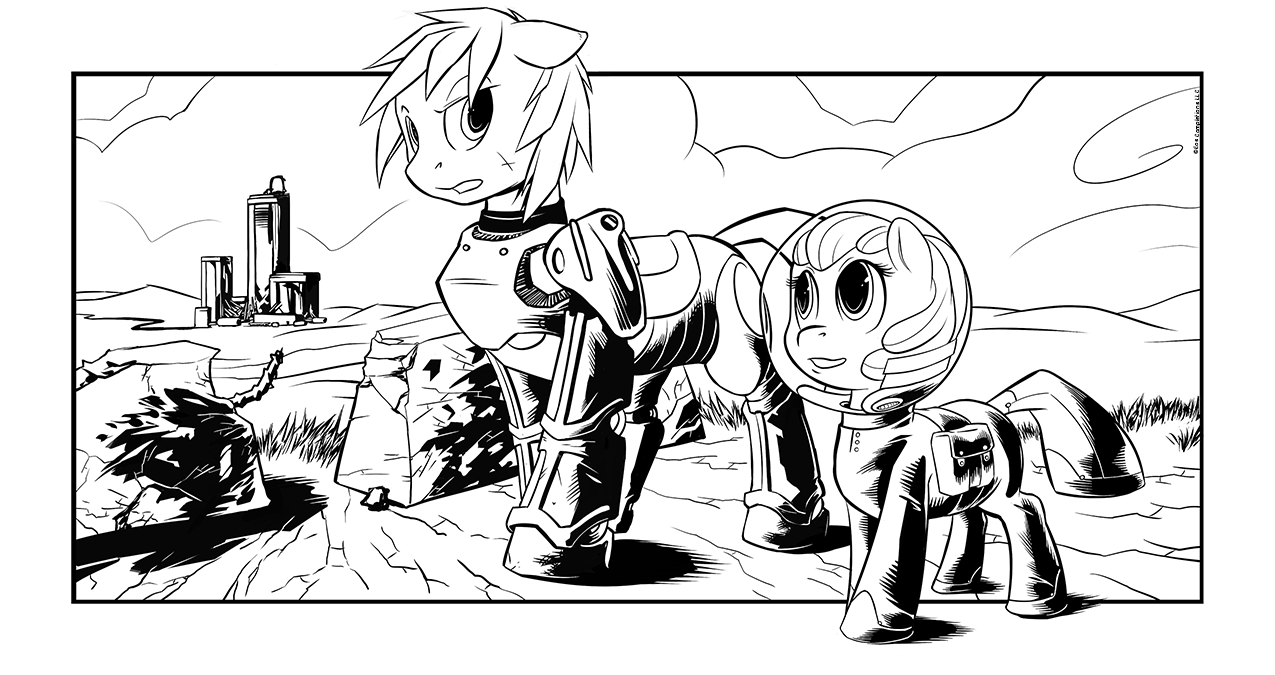
\includegraphics[width=0.9\linewidth]{image13.png}

\begin{intro}
我说,你见过下雨么?
\end{intro}

\daytimeplace{11}{18:00 PM}{象牙塔,52号国道中段}{Ivory Tower, Big 52 SC Branch}

象牙塔是个强化陶瓷外墙的巨大白色建筑。在战前这里曾经是个研究设施,和平部的员工在这里寻找神秘科学部\footnote{神秘科学部(Ministry of Arcane Science):大战时期由暮光闪闪成立的部门,负责魔法研究,\emph{FoE} 中的天角兽「女神」便是该部门的「产品」之一}和战时科技部\footnote{战时科技部(Ministry of Wartime Technologies):大战时期由苹果杰克成立的部门,主要通过陆马(物理)方式研发和制造科技产品并用于战争}研究成果的非军事用途。

现在象牙塔是铁骑卫在52号国道的唯一据点,主要因为这里是附近唯一没有被旭日公司碰过的高科技设施,而稍微有些理智的小马都不会碰旭日公司。

没错,旭日公司,那些疯子,他们将一个收音机和一个吸尘器组装在一起做成了第一个声波武器然后交给一个稀里糊涂的女仆。还发明了第一个带有窃贼监测消灭功能的门铃——这个门铃电死了六十多个上门服务小马和一整排的卖马芬小孩子。

整个建筑都被一道带有护城河的城墙围着,并且带有自动炮台和地雷阵。这个城墙经过一个世纪对抗从土匪到山贼的战斗之后。现在看起来相当糟糕。炮台早已经被摧毁,地雷阵也基本没有了,就连城墙也饱经创伤。在唯一还算完好的护城河之上有两座吊桥,一座在西边一坐在北边,在吊桥外面有各式各样的棚屋,大多都是一些旅行商队的仓库以及那些和铁骑卫做生意的小马过夜歇脚的地方。

不过现在北边的棚屋已经基本被拆光了,而各种垃圾被收集起来在桥北边堆出一个路障,同时西边的那些战前建筑也被垒上了沙包,并且飘扬着苹果杰克卫士的旗帜。

这个小小的要塞被一打小马守卫着,其中甚至还有一些穿着战斗鞍的年轻小马。一对武装到牙齿的铁骑卫穿着它们传统的动力装甲正守在桥头。另外一个则带着新兵在象牙塔周围的乱石滩巡逻。第四位则站在临时指挥所里面和一个年轻的佣兵争执着。

「你说的我能做到,但是我现在想先要一半定金,还有一些等离子武器。」赫瑞塔抱着双臂坐在椅子上,把自己的狮子腿翘在桌子上。

那个骑士一脸不爽地摇了摇头:「你当我是啥?卖房车的?我给你一柄动力长矛已经算你好运了,其它的东西只有你完成工作才给你。」

赫瑞塔轻蔑的哼着,「我是个枪手,你那花哨的肉搏兵器我用不上……给我三个离子手雷,现在给我两个,回头再给我一个,还有俩EMP地雷我就依你。」

「给你俩EMP手雷,事成之后再给你一个离子手雷和离子地雷,最终价。」小马用蹄子指着狮鹫说。

赫瑞塔耸了耸肩,抓住那只蹄子握了握,「成交,先付一半瓶盖。」

「然后你拿着钱飞走?我才不信你,而且你现在拿着钱又啥也做不了。」

狮鹫叹了口气:「你知道我怎么想的吗,我觉得你没有那么多瓶盖,你是想让我去捣乱,然后你们正面进攻,最后你们用基地里面的钱付给我……我不觉得你们四个铁骑卫和十五个新兵能够正面攻破一个至少一打半重装备小马防守的城堡。」

那个帕拉丁举起了蹄子,「好吧好吧,你这个守财奴,现在就给你一半瓶盖!别觉得我会因为这件事情感谢你。」

「谢意买不来子弹,我想这可以成交了,」狮鹫又耸了耸肩,「我马上就出发,希望你的手下别把事情搞砸了。」

「你干完活回来和书记梅隆说,如果你想参加正面进攻的话,我会再给你点别的,比如一些收集到的装备。」

赫瑞塔还没开口,但是她面前的小马举起一只蹄子示意她等等。

「冷浴收到,请报告。」小马压低声音,但是狮鹫竖起耳朵也能听得很清楚。

赫瑞塔坐在桌子面前打着哈切,不管怎么这事情和她无关,等到入夜他就出发,想想他们已经允许她从铁骑卫尸体上扒装备了,说明这些小马已经没什么选择了。

「再说一遍?你射杀他多少次了?」那个帕拉丁惊讶的叫起来:「高斯我觉得你不可能杀死一个东西两次以上……」

听到这句话赫瑞转头看着那个用对讲机说话的小马,不过现在冷浴完全没有注意那个佣兵。「你到底想要说什么,你确定那是敌军么?」帕拉丁停顿了一下听着对面的回答然后说:「所以,你只是因为觉得他有点诡异所以就开枪了?」

狮鹫听到这句话跳了起来:「肏你娘,告诉你的手下不准欺负帕比!」

\horizonline

\daytimeplace{11}{18:30 PM}{象牙塔,52号国道中段}{Ivory Tower, Big 52 SC Branch}

黄色的小雌驹,蹦蹦跳跳地来到小小的前线,看着那锈迹斑驳的路障,对上面的卫兵说:「嗨漂漂马!我叫快乐帕比,你看到我妈妈了么?」

内心和身上铠甲一样上锈的卫兵疲惫地看着帕比——他已经被连续几天无休止的战斗折磨得痛苦不堪,而且和他战斗的并不是强盗或者奴隶贩子,而是他曾经的挚友和老师。而这个小雌驹却一点都没在意对方的情绪。

帕比继续和护送她的卫兵讲着自己的故事:「……所以,即使镇长要赶走了机械战马,他还是决定去拯救城市。因为……你懂的,机械战马并不只是个机械,他也是超级厉害有正义感的小马!」小雌驹完全没有注意到那个卫兵不断上升的不耐烦情绪,「但是我刚看到那里妈妈就关了电视不让我看了,我不知道为啥她不允许我看那种电影,你说,机械战马绝对是个好马,所以最后她一定会赢,是吗是吗?」

帕拉丁高斯重重叹了口气:「对,你说的没错,不过我并不是你说的啥机械战马,我是阿杰铁卫!完全不是一回事!」

帕比咯咯笑起来,「你真有趣,机械战马阿杰铁卫!我喜欢这个名字!」

「好吧,……随你便,摆脱,至少把那个肉食灵尸体放起来,恶心死了!」小雌驹还背着那个死去的肉食灵,没有一位小马会对这个已经没有一只腿和一只翅膀的前肉食灵感觉到一丝的怜悯之情,不过小雌驹还是把它当宝贝一样带着。

帕比皱起眉头,「但是小毛球肯定也想看漂漂马,他会乖乖坐好的,我发誓!」

帕拉丁以蹄覆面,「尸体当然会乖乖坐好,但是……哎……恩……这附近有专吃宠物的怪物,所以可能会……」帕拉丁心中默默地对这个幼驹扯谎而自责。

「吃宠物?在哪儿?毛球很危险!」小孩子马上把那个小肉食灵塞进背包里面,睁大眼睛看着周围。「在包包里面躲好,我来收拾他们!」

高斯看着刚好撞上的仨随从笑得满地打滚,哑口无言。而帕比也一起笑起来,「什么事这么有趣?」

高斯避开他们的视线,拿出自己最正经的表情,「这才对,你要小心哦,吃宠物的怪物哪里都有!现在跟我去见长官吧。还有你们仨!别在那里傻笑了,赶紧给我看大门去!」帕拉丁走过那几个年轻随从,小黄驹屁颠屁颠地跟在后面。

「好的好的,阿杰铁卫机械战马!我们什么时候去打击罪犯?」

「我再说最后一次,我的名字叫高斯,帕拉丁高斯!」公马叹息着,「我绝对不会要孩子……」

这对活宝终于走到了指挥部,公马打开门让帕比先走了进来,这个建筑曾经是一个学校,不过现在大部分都已经坍塌,只剩下几个房间还勉强保持完好,在这个小小办公室的另一边坐在桌子后面的是另一个穿着铁甲的小马还有赫瑞塔。

「赫瑞!」帕比开心地一蹦三尺高,径直飞扑向狮鹫,而后者侧身闪开,然后抓住帕比的后颈将她拎了起来。帕比微微挣扎了一下,来回张望着寻找着她的朋友。「嘿,你跑哪去了?」

「我说了『再见』就是改天再见面的意思,你还在往南走么?」狮鹫一边说着一边把帕比放下,拍了拍她的头盔。「帕拉丁伙计,这个是我的老朋友,在我干活的时候能帮我看好她么?」

冷浴歪着头一脸疑惑地看着小雌驹,「这个……小马被射中四次但是看起来毫发无伤的样子,而且她看起来心情不错,我不太清楚我能不能照顾……高斯,叫诘责书记进来。」

帕比并不太关心那个帕拉丁,因为见到赫瑞实在太开心了,「没错哦,妈妈就在桥对面的那个白屋子里面!我路上看到好多漂漂马,还有阿杰铁卫机械战马!」小雌驹终于抱上了狮鹫,「我好高兴见到你,这一次你不会丢下我了吧!」

赫瑞塔清了清喉咙,避开幼驹的视线。「呃,实际上……我正要去做一些事情,不过如果你等我的话,我很快就回来。」

帕比皱了皱眉头,小心地问道:「呃……你会带上丝尾一起去么?」

「丝啥?哦,那个玩偶,当然,为啥不带他?」

小雌驹松了口气,「没什么,让它帮你吧,她很厉害!」

狮鹫拍着小孩子的头说:「很好,乖乖和铁骑卫呆着,别惹他们生气也别乱跑,我一会儿就回来带你玩,好么?」

「耶!」帕比挥着蹄子送走赫瑞,然后呆在房间里面好奇地看着其他马。

\horizonline

\daytimeplace{11}{19:00 PM}{象牙塔,52号国道中段}{Ivory Tower, Big 52 SC Branch}

诘责书记是一个常年负责训练随从的老马,他冷酷而又铁血的训练手段让每一个新兵都对他心有余悸。只有一种办法能让这个老书记看得起你,把每一个任务都完成得尽善尽美。而当他加入阿杰铁卫的时候,很多人都怀疑他的这个选择,甚至很多随从都觉得他是个间谍。

诘责一边看着帕比一边对冷浴说:「中心城尸鬼有和通常尸鬼一样的腐烂外表,我不觉得她像是其中之一。」

帕拉丁叹了口气坐在他办公桌背后,「那你觉得她是什么?她可是挨了四枪,一枪在头上,三枪心脏。」

「也能给我一个红披风么?」帕比抓着诘责的斗篷一脸惊讶地说:「我喜欢金色的东西,就像漂漂大公主的颜色那样!我长大以后我也要做一个公主!我想要这个披风,拜托!」

「这些是咒符,不是给你玩的。乖乖坐好……」诘责回头继续说。「或许是某种死灵巫术,我可以确定……如果我能去图书馆的话我可以做一些研究,不过现在我只能推测……」

「为什么我不能玩儿?我可以给你东西换斗篷!这叫做交易!超酷的!大家都这么做!不像那次我用早餐换了两块大理石然后饿得发慌被妈妈骂……这次没问题的!」

帕拉丁无视帕比,点了点头说。「那么你的推测是什么?」

诘责看了看那个幼驹然后回答:「我不想拿我的斗篷和你换什么,乖乖坐那儿让成年马说话好么?」书记官叹了口气然后继续和冷浴之前的谈话,「我记得读过这些防辐射服的故事,它们显然没什么作用,在中心城的核爆之后几乎每个穿着它的小孩子都变成尸鬼了。」诘责停下来低头看着那个不停地扯着他斗篷的小雌驹,「不过这一个,我要说……或许我给他的防护服做一次检查就知道结果了。」

老书记把他的哔哔小马接上帕比衣服的数据接口,另一个蹄子按着幼驹让她别动,「安静几分钟好么?」

「我能抱抱你么?你好有趣,我喜欢你!」帕比想了想又说。「我也喜欢你的披风,刚才我说过了么?」

冷浴忍不住笑了出来,书记官瞪了她一眼,「好吧,你想怎么抱我就怎么抱我,恩……我们看看结果……」

诘责皱起了眉头,「从数据上看她已经死了,没有心跳,没有体温,甚至都没有身体,只是……两千多个骨头碎片和一百八十克有机物,完全不是尸妖。」

「呦呵,红斗篷也会说不明觉厉的话!」

「没错,诘责,别说那些不明觉厉的话,给我一个士兵听得懂的说法,我只懂轻武器和战车。」冷浴并不是不高兴,只是想提醒一下老书记官他现在并不是在讲课。

「我也不清楚,只能说她不是尸鬼。」诘责低头看着哔哔小马上的分析结果,「这个防护服的自律智能完全没有受损,所以我可以肯定这不是一个疯狂机器……哦,这一条很有趣,主医疗芯片在两百年前就故障了,这可是千分之一的故障率,或许是因为在启动中受到了电流冲击或者短路,所以只有备用护符在起作用。

「这一条哪里有趣了?」冷浴不解。

书记冷笑一声,「因为备用医疗护符和主医疗护符有很大不同。」

帕拉丁打了一个响鼻,「请一次说完好么,我可没时间做课后复习了。」

书记叹了口气,忽略帕拉丁的态度,「这个护符并没有内置医疗法术,只是有一个自动注射医疗药水的功能……等等,这个魔法回路上还刻着其它东西,是……斑马的咒文?医疗护符上刻着斑马咒文有什么用?」

这个咒文的结果现在就站在他们鼻子下面,用力扯着诘责的斗篷,「好吧,那咒语,保存了……一百八十克有机物?」

书记官继续看着他的哔哔小马,「对,这是一个有点腐烂的心脏,我要说……这个非常有趣,扫描表示有很多破碎的子弹漂浮在心脏附近,就好像它们没有命中心脏一样,我们看看护符的日志,或许能理解它的工作原理。」

他们俩聊天的内容太无聊了,帕比虽然是一个很有耐心的孩子,但是全小马国的耐心都没有那些哇啦哇啦哇啦麻烦,所以那个黄色的小雌驹开始把自己的蹄子伸进书记官口袋里面翻起来。她找到……一支笔,几张纸,一本书,一副眼镜……咔嚓……好吧,现在是一个单片眼镜,还有另一个单片……「咦,这是什么?」

帕比从诘责口袋里面掏出一个梳毛塑料玩具,那是一个白绿色鬃毛的独角兽,脸上带着一个大大的微笑,还有一个竖琴的可爱标记。

「哦哦哦,好可爱!」小雌驹抚摸着玩偶的鬃毛,「梳啊梳,梳啊梳……」

「怎么……喂,还给我!」书记官生气地把那玩偶从帕比蹄子上抢下来,然后塞回自己的口袋去。「玩你自己的玩偶好么,这个可动手办很容易就会弄……」诘责的视线对上了冷浴的目光,然后他才意识到发生了什么,「不不不不不不……咳……这个……玩具……恩恩……是我没收别的新兵的,不是我的别玩坏了!」

帕比一下子兴奋地睁大了眼睛,「不是你的?能给我吗?我会好好爱护她,给她梳毛,一起和她玩,我们会成为最好的朋友,就给她起名字叫糖糖\footnote{糖糖和天琴,同人中默认的一对CP}然后给她染个粉毛。」

诘责听到要给玩偶染毛的话之后立刻炸毛了,「她的名字是『天琴』,而且我不能给你,因为那是我……呃……我的一个学生的,应该仔细分类保管好!」

一个贱贱坏笑出现在帕拉丁的嘴边。

「别对一个玩具那么认真嘛诘责书记,我觉得让这个小雌驹玩一个小女孩的玩具没什么问题。」

冷浴一脸黄鼠狼给鸡拜年的坏笑。

「看吧,看吧,机械战马也说我可以玩,给我嘛,给我嘛!给我嘛!!」幼驹踮着脚去探诘责的口袋,但是这一次老书记官连忙捂住了自己的口袋。

「这个是我的总行了吧!天琴是我的!我不能给你因为我喜欢天琴!你满意了吗!嗯?」按下内心自爆按钮的书记官涨红了脸看着冷浴,「你可以从这个大姐姐房间里面挑一个玩偶,我想她会让你看她的卧室的,我想她没什么好藏的东西,对不对啊,机械战警?」

冷浴咳嗽了一下收起了笑容,「好吧,我带你去找几个漂亮玩具,小家伙,不过先乖乖让书记官做完他的工作。」

在新玩具的保证下,帕比一脸开心的表情乖乖坐在那里让红斗篷小马继续摆弄她的防护服。

诘责叹了口气,看了帕拉丁一眼说:「你能不要露出那副阴阳怪气的笑容好么,我干正事呢……」书记官叹着气。

「我的天……没开玩笑吧,他们居然在医疗护符里面放这种东西?」

冷浴一脸迷茫地看着诘责。「你发现什么了?你的脸色看起来不太好。」

「非常糟糕的事情……和平部的某小马为了不让这些小孩子死而做了非常可怕的事情……她不允许他们死掉。」

「什么叫不允许?」帕拉丁抬起一根眉毛问。

「我是说,这个备份护符的最后咒语是某种死灵术,虽然不清楚具体是什么不过看起来它的功能是把患者的生命灵魂束缚在它的遗骸上。」老书记官叹了口气,「不过,这个并不是太强的法术,我想花点时间研究一下就能解除它。不过这又回到了我们之前的问题上了——我需要图书馆。」

冷浴喃喃自语着:「就算是从爱的角度出发,怎么会有马做出这种……禁止你去死的东西,这个有可能么?」

「既然结果已经站在我们面前,我觉得可能,我不是死灵术专家,但是我可以说这个护符状态并不是很好,它在两百年的时间内都只靠一点点能量维持运转……我不知道怎么解释,这个法术逻辑上根本行不通!一定还有其它拼图碎片没有找到……或许……」

帕拉丁歪着头问:「所以说,基本上这个小鬼是某种幽灵?」

诘责摸着下巴,「我不太清楚,我还是需要再研究一下,不管怎么说我觉得这个护符是关键,没有它这只不过是一件破防辐射服,一堆粉色粘液和一个小雌驹的遗骨……你如果说这就是幽灵的话,我不这么认为,技术上讲这个可怜的小家伙根本不可能站起来,但是现在她却和一个孩子一样活蹦乱跳,不管记忆上还是精神上都完全没有问题。」

老书记官顿了顿,揉了揉自己的眼睛然后继续说:「从日志上看,这个防辐射服已经停止运转两个世纪之久,然后忽然它的魔能电池就充满了远高于它最大能量的魔力。整个防护服都以五倍于它理论效率的水平运转……不管从科学上还是魔法上的逻辑都行不通,或许她是小马灵魂的某种具象化?」诘责一脸沉思的表情放开了帕比的蹄子,「好吧,小家伙,检查完了?」

帕比微笑着抬头看着书记官,「耶,现在我就去找妈妈了,回头我回来拿玩具,拜拜!」

\horizonline

\daytimeplace{11}{19:45 PM}{象牙塔,52号国道中段}{Ivory Tower, Big 52 SC Branch}

帕比用力敲着「我要去找妈妈!放我出去!」小雌驹一边哀求着一边敲着门,但是没有马理她,她被困在这间教室了。

那些讨厌的机械战马把她带到这个房间然后说要给她玩具,然后就把她关在了这里,就像商场的托儿中心一样,她讨厌托儿中心……虽然他们也给了她很多玩具彩笔甚至一个超级炫酷的彩图连环画,但是她现在不是玩这些东西的时间,她应该去找她的……「哇哦!这里画着漂漂蝴蝶!」不对,帕比,你必须抵抗诱惑……你应该……「哇哦,金色蜡笔!真的是金色的哦,我可以用这个笔画塞拉斯蒂娅公主,给她涂上金色就和真的一样了!」

不对!妈妈才是首要任务!帕比是有重要任务在身的小雌驹!她放下那些炫酷的连环画和蜡笔,这些\stpr{腐朽奢靡的花哨玩意儿}才不会让她停下脚步!绝对不会!

「咦?着是真的茶具么?还有茶杯!」

帕比一败涂地。

而五分钟之后帕比已经输得找不到北了。

「天啊,毛球小姐吃了瑞瑞女士的万马奔腾庆典礼服!如果没有金色蜡笔的话整个庆典就完蛋了!不过没有关系,漂漂塞拉斯蒂娅公主带着金色蜡笔登场了!还有云宝黛西!庆典得救了!大家一起喝茶庆祝吧!耶!」

帕比举着肉食灵尸体和其它玩偶,自言自语地着专注于她想象中的场景——那个完全变成茶话会的万马奔腾庆典。

诘责看着窗口里面的情形耸了耸肩,「看起来她不会惹什么麻烦,让两个侍从守着大门以防发生什么意外,我们继续准备今晚的进攻计划吧。」

冷浴浑身不自在地跟在诘责的后面,「她看起来暂时有点乐不思蜀,不过这不是长久之计,我们不可能就这样把她关在这里,过不了多久她就又会吵着要找妈妈了吧。」

老马叹了口气:「我想我可以解除她身上的诅咒,那个咒语很弱,不过我还是需要研究一下斑马魔法,而且还需要几个独角兽配合。」

「那样的话……她会死么?」帕拉丁的声音里面充满担忧。

诘责疲惫地转过头,一副沉重的表情严肃地说:「她已经死了,冷浴,这个小家伙现在需要的是安眠,她本来就不应该存在。」

「但是,她又不在乎……我们至少应该找找看她妈妈是不是还活着,或许她变成了尸鬼……如果她还活着,或许图书馆里面会有一些记录。」

书记官耸了耸肩,「那么又回到了我们之前的话题,夺回我们的基地还有图书馆,所以说,找俩侍从看好她吧,我们现在应该讨论一下如何解决眼下的问题了。」

\horizonline

\daytimeplace{11}{22:00 PM}{象牙塔,52号国道中段}{Ivory Tower, Big 52 SC Branch}

再来点粉色云彩……完成咯!帕比开心地看着她的新创作,谁说不能用粉色画画?把所有东西都画成粉色不就行了吗?她拿起来这幅画把它和其它的画贴在……{}

轰隆!

整个窗户颤抖了一下,外面的光芒透过窗户在地板上照出不详的橙红色方格,让帕比惊讶地站住了。

「烟花?」

轰隆隆!

外面又爆出一团红色的火球,窗户整个炸碎了,玻璃的碎片飞得满屋都是,桌子上和帕比的头盔上都是,不过帕比完全不在意,她探出头去好奇地看着外面发生的事情。

「耶!烟花大会!」幸运的帕比这次赶上了漂亮的烟火!就在桥对面,好多好多小马在跑来跑去玩着烟火,相互丢着各种颜色的光线和烟花,果然那些机械战马知道怎么开个超级大派对!

幼驹走到门口才想起来门被锁上了,不过这阻止不了帕比,她直接从窗户跳了出去。

脚踩在外面的地面上,黄色的幼驹稍微迟疑了一下,把那么多玩具和画丢在那里实在太可惜了,软气那次怎么说的来着?总有一天她需要作出牺牲……如果想要前进就要把某些东西留下。帕比就知道那些丑丑马很厉害,又聪明又厉害,还有乐乐姐姐也是!所以她是个有重任在身的小马,而且她也想去看烟花,所以……再见了!漂漂玩具,再见了!蜡笔!哦,她要先去找妈妈!出发!帕比!

\horizonline

\daytimeplace{11}{22:15 PM}{象牙塔,52号国道中段}{Ivory Tower, Big 52 SC Branch}

象牙塔和大桥桥头之间的整个区域都变成了一个战场,四个阿杰铁卫在用他们的重武器压制着对面阵地,而其他侍从则发起进攻,那些只有轻武器和少量铠甲的新兵用血肉之躯发起冲锋,而当帕比穿过大桥的时候,从帕拉丁高斯身边晃过去的时候他完全没有注意到黄色小雌驹。

「肏你妈,她在这里干什么?冷浴!幽灵在战场上!」帕拉丁想追上帕比,但是刚露头就被一阵凶猛的火力压回了掩体,「肏,这尼玛出去就是死路,而且不止一条!第二小队需要掩护!」

帕比看到一个年轻雌驹躺在一个冒烟的弹坑旁边,一滩红色的液体正在那静静安睡的年轻雌驹身体下面慢慢扩大。

「喂,漂漂马,你还好么?」帕比看着那个侍从,她虚弱地睁开眼睛。

「请……救救我……我……我不想死……」士兵的声音虚弱得几乎听不到。

小雌驹轻轻抚摸着侍从的鬃毛。「别害怕,烟火是有点小可怕,但是你是个成年马不应该哭的。」

濒死的小马迷茫地看着她,没有听到幼驹安慰的话,「我……我不想死……」她如此年轻,或许才是第一次参加战斗的新兵。

「好了好了……」帕比坐在小马身边,不停地摸着她的鬃毛。「我陪着你,别害怕,已经没有什么好害怕的了……等烟火结束了我们去买棉花糖,好么?」

帕比第一次看烟花也很害怕,但是妈妈给她买了棉花糖她就不哭了,或许这个小马也一样,给她买个好吃的棉花糖她就不哭了。有几发流弹打在帕比身上,但是她完全没有注意。

「妈妈……抱歉……为什么我要离开家?」侍从低声说着她最后的遗言。

「呃……别担心漂漂小马,如果你离家出走妈妈一定会很高兴在看到你的……或许她会训斥你,但是我保证她会抱抱……」但是那个小马并没有回话。

帕比轻轻戳着她。「呃,你还好么?漂漂小马?呃……声音先生?她还好么?」

「{\mt 分析中,否定。阿杰铁卫侍从状态:已死亡。}」

帕比皱起了眉头,「哦,像是赫瑞的爸爸……」帕比似乎终于意识到发生了什么。「声音先生……这些小马在玩还是在打架?」

「{\mt 这些小马在战斗,不过双方都未将你标记为敌对,只有固定防御系统标记为敌对。}」

似乎是要强调那句话一样,爆炸的弹片飞过,打裂了帕比的头盔。

「{\mt 警告,密封失效,修复护符起动。发现敌对目标,数量:2}」

「嘿!不要拿着那些东西乱指马!」帕比站了起来,把死去的马丢在一边走向旁边一队把一个翻倒的汽车当掩体的侍从,「别打架了!很危险的!你们的朋友病得很重!」

一个士兵看着黄色的雌驹惊呼道:「你这死丫头在这里干啥?快趴下!」

小幽灵歪着头,一脸疑惑,「为啥?」就在这时候,一发子弹穿过了帕比的臀部,流下一滩粉色的液体,就好像她是黄油做成的一样。

侍从惊恐地看这一幕,而帕比则冲着炮台大叫「不准欺负马!」他们看起来完全不知所措。那些士兵眼睁睁地看着小雌驹径直冲上了最前线。

「停!停下来!好危险的!不准欺负马!你们没看到大家都被你们吓坏了么?」

帕比大叫着冲向象牙塔的入口,而那里一对铁骑卫正在拼命射击着进攻的侍从。其中一个看到小雌驹然后向她打出一发榴弹,把她炸飞到了一边去,帕比花了一分钟才完全恢复,这个时候冷浴已经冲到她身边。

「帕比你在这里干什么,回学校去!」

帕比摇了摇头,「才不!我不喜欢小马吵架,更不喜欢打架,大家应该和平相处,暴力是不对的!」

帕拉丁叹了口气,「这是战争,帕比,你抱怨也不可能停止战争,这是我们的事情,别担心,回学校去,这里很危险!」

「啊哈!没有什么战争是太空战士安德洛队长解决不了的!」幼驹高举起蹄子大喊到:「激光枪!」那个颇具卡通风格的小枪出现在她面前。

冷浴想抓住帕比,但是一排子弹逼着她躲回掩体,「把那个玩具枪收起来跟我走!听见了么帕比?帕比!」

小雌驹悠然走到战场的正中间,然后举起枪对准大楼的入口,「立刻停止战争然后投降,不然我要开枪了!你们这些坏蛋不觉得羞羞脸么!」

一个自动炮台打中了帕比的腿和肚子,而其他铁骑卫只是忽略她的存在,冷浴拼命想找个机会从枪林弹雨之中把幼驹抓回来。

「好吧,好吧,你们自找的,太空战士安德洛队长,飞向星空宇宙无限!」幼驹就好像躲着看不见的子弹一样弓起身体,接着举起那把「玩具」枪,然后说:「乒!」

然后又说了六次。

「乒!乒!乒!乒!乒!乒!投降吧!异形斑马!」

「{\mt 目标一号到七号定位完成,到普罗米修斯中继站二号的通信链路连接完成,普罗米修斯状态:完全可用,传送坐标。}」

在那座大楼三层的窗户忽然爆炸了,而狮鹫一边向里面开枪一边飞了出来,帕比立刻看到了飞出来的狮鹫。

「{\mt 普罗米修斯一号、四号、五号、九号、十号、十一号以及十二号完成设计准备,普罗米修斯二号、三号、六号、七号以及十三号无法瞄准地平线后目标,使用间接瞄准模式,校正时间:30秒。}」

「赫瑞!赫……瑞……!我在这儿!拜托让他们别打架了!赫瑞!」帕比四个小蹄子猛蹬着追在狮鹫身后,还拿着玩具枪,身后还有个炮塔在打着她。「等等!」

傻小鸡!帕比觉得自己需要一些东西来引起她的注意,于是她收起来枪然后举起石块,瞄准——精准命中!狮鹫打着转从天上降落——好吧,是坠落在了小雌驹不远处。

在无尽的黑暗太空之中,普罗米修斯睁开了它的毁灭之眼,半打红色的光线指向那幢建筑,开始看起来那些只是穿过云层的细线,但是很快那些激光开始聚焦,变成了红色的激光,在浓烟滚滚的夜空上划出无数光柱,就好像来自天堂的红光正咬着白象牙塔。

「撤离!立刻撤离!所有小马离开你的位置撤离战场!」诘责被魔法放大的声音盖过所有炮弹的爆炸和呼啸,所有侍从开始听从诘责的声音撤退,从他们的掩体里面出来飞奔向大桥另一段,而防御的铁骑卫则停火看着大军撤退。

「帕比你丫的又拿石头砸老娘是不是?」

赫瑞塔揉着头上的大包说:「那老木乃伊在瞎嚷嚷啥玩意?」

帕比一下抱住了她的朋友,「不知道,不过我想让你告诉他们别欺负小马,不过看起来他们已经不闹了。」

「{\mt 所有武器阵列瞄准完毕,目标锁定,开始倒计时……十……九……}」

\clearpage % NOTE: 此处不能在前面那页放下

~\vfill

\begin{note}
    升级(Lv 12)

    新技能解锁:小小扒手——帕比,还给我!你在偷窃时更不容易被抓到,并且你可以在对话时打开其他NPC的物品栏。
\end{note}




\chapter{玩偶}

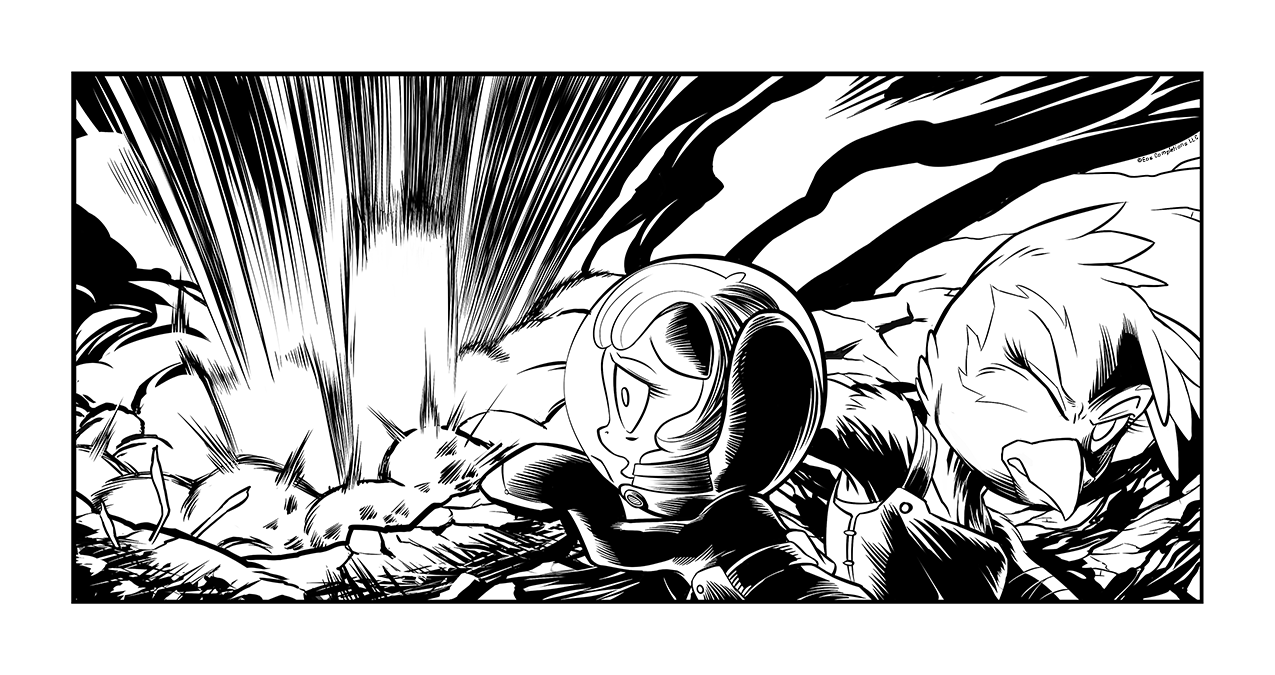
\includegraphics[width=0.9\linewidth]{image14.png}

\begin{intro}
    人生必有不可避免的阴雨日
\end{intro}

\daytimeplace{11}{22:30 PM}{小马国上空约 \SI{1800}{km} 近地轨道}{Low orbit, $\approx \SI{1800}{km}$ above Equestria}

在行星上空轨道上运行着的是普罗米修斯——一个巨大的超轻合金马造奇迹。它的形状就像一个巨大的向日葵,长长的太阳能电池板在它四周伸展着,在它的外壳上画着很多标记,比如说流星,辐射警告等等,但是最显著的还是旭日公司的标记,一个大大的天角兽,下面有一行走「可持续发展道路」的字样。

在卫星的圆形主体上,有四个巨大的圆管,长度比一列火车都要长,这些巨大的武器被金属环固定在一起。这圆管里面是被称作质子炮的武器,它使用强大的魔法电磁混合力场,是将巨大等离子团加速到近乎光速投射向超远距离目标的致命武器,每一门都有巨大的破坏力,而每一个卫星上装着四门这种「玩具」。

不过旭日公司可不是做事做一半的小马,一个这样的卫星怎么可能在需要的时候随时发射呢?所以这个卫星一共有十一个伙伴,全都零零落落地分部在小马国上空的卫星轨道组成了一个卫星网络,就像一串明亮的珍珠项链一样。而现在整个家族都将炮口指向地面,明亮的引导激光照向它们的标靶。

「{\mt ……八……七……六……}」

随着倒数计时,每一个炮管口都亮起了蓝色的电离光芒,长长的两根伸出来的磁轨就像是不详的朗基奴斯之枪,而魔力场和磁力场包围在磁轨上形成一圈圈的蓝色光环。

「{\mt ……五……四……三……}」

在卫星背后,四个舱门逐次打开,开始喷射推进剂用来抵消武器系统的巨大后坐力对轨道的影响。那些碗状的喷口之中首先是有一个红点,然后立刻像是火山口一样猛烈地喷出火焰,而前面的四个炮管已经完全被蓝色的光芒覆盖,魔力和磁力在圆环上来回流窜,随时准备释放他们的狂怒。

「{\mt ……二……一……发射!}」

\horizonline

\daytimeplace{11}{22:30 PM}{象牙塔,52号国道中段}{Ivory Tower, Big 52 SC Branch}

「{\mt 攻击确认,第一波轨道轰炸降落时间:7分钟后。}」

半数的引导激光消失了,还有一些在疯狂地摇晃着,好像是天堂发生了什么可怕的事情,但是依然有五道光柱紧紧锁定在目标上。

「为什么大家都开始撤退了?」

赫瑞塔展开翅膀,准备抓起帕比立刻飞走。

黄色的小雌驹指着基地入口说:「那里有俩没跑的,我们去问问他们?」她一边说着一边走向那守卫着大门的俩帕拉丁。

「这可不是个好点子!我的活已经干完了,我们最好跟着我们的好伙计一起跑。」

「{\mt 警告建筑物内的所有小马!你们已经被轨道轰炸瞄准!立刻离开,我们不会向你们射击,请快逃命吧!}」诘责的声音再一次在战场上回响着,然后他也跟着其他学徒和抄写员一起掉头跑。

抬起头看到那刺破夜空的红色引导激光,赫瑞惊讶地张开了喙,「你妈下的臭蛋……如果这激光只是用来瞄准的话,我可不想看它射击。」

「{\mt 警告,普罗米修斯三号,五号,十号,十一号和十二号失去信号,普罗米修斯四号和七号反推系统严重故障,普罗米修斯一号,二号,六号,八号和九号攻击完成,准备第二次,倒计时……九……八……}」

帕比皱起了眉头,声音先生从刚才开始就一刻不停的说着莫名其妙的话。这让幼驹对现在的状况更是丈二和尚摸不着头脑。面前大家都在逃命,红斗篷先生又在大叫着什么,而她的头盔上到处都是红色的警告灯。

「怎么才能把这一团乱停下来?」

「我不知道,我也不关心,我们快跑吧!」赫瑞抓起帕比伸开翅膀开始逃命。

不过马上又有个新的问题,飞行。帕比已经做好下一次飞行的准备,在下一次飞行的时候有一件事是不得不做的,是什么来着?对,是尖叫。

「咿……!别!别!不要!不要!」

「给老娘闭嘴!你丫想活命吗?」狮鹫被沉重的小雌驹拖着,完全飞不起来。

「你丫身上到底装了什么,前几天我刚让你丢了十吨的垃圾,现在你身上又都快装满了?肏!快把东西丢了,要不我们会坠机的!」

「{\mt ……二……一……第二波轰炸发射,开始准备第三波轨道轰炸。}」

「放我下来!放我下来啊啊啊啊!」帕比因为面前双蹄之间的地面距离自己太远而且移动速度太快而大声尖叫。

赫瑞塔用爪子抓着小雌驹的一只鞍带,在用力划了几次之后,终于在上面划出一个长口子。

「搞定」

「{\mt 启动修复魔法,普罗米修斯一号,二号失去信号,普罗米修斯六号,八号和十一号继续射击,倒计时……十……九……}」

物品管理系统把所有东西都固定好的同时,自动修复系统立刻补好了袋子上的大洞。

「喂,这也太诈了吧!你丫玩老娘是吧?看招!」狮鹫抓着帕比的一边把她倒了过来,这个方法看起来奏效了,因为她的包包没有扣好,小雌驹的体重迅速减轻,而身后则洒落出一长串东西,空瓶子,烂玩偶,小小的玩具车什么的。

「呀!呀!呀!不!停下!拜托放我下来!我要吓尿了!」但是这个方法同时也让帕比的飞行恐惧症更加糟糕,不过幼驹还是在「命运之石」掉出包的时候抓住了它,虽然小雌驹找到的其它好东西都已经丢了。今天真是个坏日子,而且这个蠢赫瑞塔还在欺负她。「你这个讨厌鬼!放开我!我要告诉我妈妈!」

终于帕比的体重达到一个可以承受的标准,赫瑞把小雌驹背回了背上,希望能减轻一下雌驹的惊叫声。「好了好了,已经搞定了,现在能安静坐好么,飞过那个山头我就把你放下。虽然赫瑞不知道天上会掉下什么,不过佣兵的直觉告诉他有一个掩体非常重要,虽然很奇怪到现在为止还没发生什么事情,不过一般来说,大招的蓄力时间越长威力也越大不是么?「我们现在还不能降落,帕比你不要去想飞行的事情,闭上眼睛听音乐好么?」

帕比听到之后,觉得这个音乐的主意看起来不错。

「请打开音乐!」

在下面的小马拼命逃命的时候,广播声响了起来,两个不同派系的铁骑卫现在都相信老书记官的话,迅速跑向山丘。

「{\rt 女士们,先生们,晚上好!坏孩子们还没睡觉么?孤狼的52电台给你带来新鲜的52新闻!既然我们有很多事情要讲所以我们还是先切入主题吧!}」

为什么不是音乐?为啥每次帕比打开收音机都是这个罗里吧嗦的小马在念?帕比想要音乐!而现在地面已经是一个快速划过的残影,而声音先生也在唠叨着什么奇怪的东西。帕比想要哭,而在防护服的背景音之中,声音还提示着剩下的三个卫星依然在继续攻击。

「{\rt 首先是第一条:南岸的事情开始变得一团糟,看起来土匪又在铁毡附近的路上出没,不过这一次他们看起来比之前装备更加精良也更加有组织,或许他们有了新的领导?这只表示将来会有更多更大的麻烦。如果你们在花椰菜镇南边的纪念碑和铁毡镇之间旅行的话,千万要小心,而且避免走通向翠绿海滨的路,沿着大路赶快赶路,小心驶得万年船!}」

狮鹫快速地飞过夜空,轻松飞跃那些还在逃跑的小马,虽然她还不太明白为什么所有小马都在逃命,不过赫瑞还是背着快把她勒死的帕比快速飞离。

「{\rt 而且祸不单行的是,我们还收到另一条来自NCA的政令,高兴么?NCA现在认为每个旅行商都是土匪,他们开始逮捕旅行商,如果你计划往那边走的话,建议你重新考虑一下是否需要去岩块城或者通道镇来做买卖,毕竟现在52号国道北边还算安全。}」

赫瑞塔降落在山坡背后,大口地喘着气,帕比一看到坚实的地面就立刻从她背上跳了下来,对那个坏小鸡吐着舌头,「哼!为啥老是欺负我!我还是你朋友呢!」

「滚边去死丫头……」赫瑞上气不接下气地说:「老娘才没欺负你,那边不知道要发生什么……发生什么很糟的事情。」

「{\rt 然后是最后一个新闻,看起来一个老商人从他长长的路途回来了,他四年之前带着一个双头牛拉着整车的垃圾出发,而回来的时候带着……好吧……还是一个双头牛和整车的垃圾,还有一箩筐的故事,或许改天我可以和你们讲讲他所拜访的那些城市。他说远处在河的对岸有一个灯火通明的大城市,还在河上建了一个大坝来发电……哇哦,或许我们这里可以考虑建一个\footnote{\emph{FoE: PH} 的剧情}?好了,晚间新闻播报到这里,来点音乐吧!}」

帕比好奇地歪着头,「发生什么坏事?但是我妈妈在那里!」幼驹转向象牙塔,现在那个建筑已经在几公里之外,被红色的引导激光微微笼罩上一层诡异的颜色,于此同时它上面的云层忽然变得明亮。

这个时候收音机开始播放音乐了。

\begin{music}
雨滴不断落在我鬃毛上

Raindrops keep falling on my mane,

\medskip

就像是一个幼驹没有可爱标记

And just like the foal whose cutie mark is not there,

\medskip

什么事都不顺利

Nothing seems to fit there.
\end{music}

纯白的光之长枪穿破云层,径直刺向红色的靶心,那些光束重重地砸在白色的象牙塔上,冲击的力道就连站在这么远赫瑞塔都感受得到。

\begin{music}
雨滴不停落在我鬃毛上

Raindrops are falling on my mane.

\medskip

雨不停的下——

They keep falling---
\end{music}

被击中的建筑物首先是被一道纯白的光芒所包裹,然后建筑的外墙似乎膨胀了一些,看起来就像是气球做的一样,有那么一瞬间那象牙塔看起来就像是要飘起来一样,但是下一瞬间它就炸成了无数的碎片——墙,窗户,大门……就像是妈妈给她看的某个展示房间零件的滑稽画册,接下来那些零件开始四散飞去。一块块外墙就像纸片一样被炸飞上天,整个象牙塔看起来就像是个纸片城堡一样被炸得四分五裂。

在这之后声音才传来,帕比一开始听到的是一阵尖锐的呼啸声,就像是用蹄子在玻璃上划发出的声音一样,在长长的呼啸声之后就是轰隆的巨响,不过不仅仅是一个「轰隆」,而是持续不断的轰隆声,就像是滚滚天雷一般。

帕比希望妈妈能在这里和她一起看这幅景象,真是太有趣了!不对……等等……妈妈在……妈妈应该在哪个漂亮的白色建……哦不!

小雌驹瞪大眼睛举起蹄子指向曾经是象牙塔的地方,她的表情被惊恐所覆盖。

「妈妈?」


\begin{music}
    所以我和太阳公公讲理
    
    So I just did me some talking with the sun,
    
    \medskip

    我不喜欢它的做法
    
    And I said I didn't like the way she got things done.
    
    \medskip

    因为它没有认真做事
    
    She's sleeping on the job.
\end{music}

「{\mt 警告,普罗米修斯六号弹药已用尽,其它卫星信号丢失,攻击停止,目标区域将会在15分钟之后恢复安全。感谢您选择旭日科技作为您的主要火力覆盖武器。旭日科技——走可持续发展道路。}」

% NOTE: try the alternative. ???

帕比目不转睛地看着那白色的光点穿过云层不断落在她的任务目标上。为什么还不停下来?什么时候才会结束?那东西已经弄出很大噪音了,应该停止了,不是么?如果只是一下下烟火的话还算有趣,但是现在有点……可怕。帕比屏住呼吸,拼命祈祷着,希望每一个落下来的光线都是最后一道,但是马银色的光雨却违背她意志不停地落下。继续蹂躏着声音先生说的妈妈缩在的地方。

不过……等等!那个箭头,那个箭头还在!希望还在!帕比欢呼着,没有什么可以阻止妈妈,知道厉害了么光雨!


\begin{music}
    雨滴不停落在我鬃毛上
    
    Those raindrops are dropping on my mane.
    
    \medskip

    雨不停的下——
    
    They keep falling---
\end{music}

另一波光雨就像是流星一般穿过云层砸在废墟之上,这一次似乎击中了研究中心的发电厂,因为这一次冲击伴随着一个巨大的绿色火球并且腾起高高的蘑菇云直冲天空。

「{\mt 警告,检测到微量辐射,威胁等级:可忽略。}」

罗盘上粉色的箭头闪烁了三次然后消失了。帕比等待着它再一次出现,希望它再一次出现,祈祷着它再一次出现!但是罗盘还是空空如他,防护服只是通知她任务『追雨』已经完成。

为什么那些银色的东西还在落下?已经结束了,全都结束了……箭头没了,妈妈没了!妈妈……已经没了?不……不可能!妈妈还……妈妈一定还在箭头指的地方……但是……但是现在箭头也不见了!帕比一直跟着箭头,因为那个箭头指着妈妈在的地方,但是现在箭头不在了,再也没有地方可以去,再也没有什么东西剩下……只剩下一堆坠落的繁星……在离开中心城的第一次,小雌驹不知道该做什么。

妈妈不在了。


\begin{music}
    但是我只知道
    
    But there's one thing I know.
    
    \medskip

    那些从天而落的忧郁
    
    The blues they sent to meet me,
    
    \medskip

    绝对不会打败我
    
    Won't defeat me.
\end{music}

帕比大睁着眼睛,幼驹完全不动了,空洞的眼睛看着前方,脸上露出惊讶的表情。

赫瑞塔拍着小马的肩膀,想要在隆隆的爆炸声之中说点什么,不管天上落下来的是什么,现在地面上估计已经什么都不剩下了,但是就算刚刚发电机的爆炸之后,那些炮弹还在不停地落下来,那些家伙只是在浪费弹药而已。

「别担心!你的妈妈不在那!我去里面看过!她不在象牙塔!」

但是帕比没有反应,小雌驹甚至没有听进去一个字,赫瑞用力摇着她,但是小雌驹没有一丝反应,只是像一个坏掉的玩偶一样,脑袋在头盔里面晃来晃去。


\begin{music}
    没有什么值得让我伤心
    
    It won't be long till happiness steps up to greet me.
\end{music}

「别这样帕比!你经历过比这糟糕得多的事情,喂喂,有在听我说话么?」赫瑞戳了戳小雌驹,只是让她的头像摇头娃娃一样晃来晃去。「怎么回事?醒来啊!」但是还没有反应。

「我们赶紧离这里远点,最后那爆炸把放射性尘埃喷得到处都是,」年轻的佣兵无力地叹息着,「为啥是我!我只是接受个简单的工作而已,为啥每一次我想干点儿啥事都要去南边!好吧,我才不想知道为啥!」赫瑞把帕比背在她背上,急忙想追上铁骑卫。

「不管怎么说,那些家伙还差我一半工钱,我们走帕比!」狮鹫慢慢地走着,总是觉得不对劲,「我可受不了你这个样子,说点话好么?」还是没反应。

「好吧,你想要我来硬的?那么我来硬的!」赫瑞塔抓起帕比的一个蹄子晃着,捏起嗓子学着她朋友那聒噪的音量,「好啊!我们走,漂漂坏狮鹫!」

不过看起来攻势开始慢慢减弱,只剩下零星的几道光线穿过云层落在地面上。

「真棒,现在我在和一个大木偶聊天……老娘真他么开心……」

\horizonline

\daytimeplace{12}{4:30 AM}{铁骑卫前哨站,52号国道中段}{Steel Ranger's Outpost, Big 52 SC Branch}

一队铁骑卫,包括书记官还有侍从驻扎在上脚下的一个营地,他们正在从建设在山内部的一个碉堡里面搬出各种箱子。

这个小小的碉堡在战前曾经是一个观测站。而在一个世纪之前这里就成为了铁骑卫的前哨。整个建筑建设在山内部,顶部还有个高高的观测塔楼,不过里面的空间只能容纳一个排的士兵,虽然这个设施很小,但是作为铁骑卫存放补给物资的地方是再好不过。

「你看,事态明显已经超出预期,我现在真的是一个子儿都没有了。」招呼赫瑞塔的冷浴忙得都没时间脱下头盔。

狮鹫轻蔑地哼了一声,「老娘干了活了,他们的发电机和内部防御系统都已经干掉了,不管那基地是不是给流星砸了,老娘现在就要赏金!」

「你可以去那弹坑里面找你的赏金去,想拿什么拿什么,我现在还有个营地要建设,还有一大堆杂事还有一堆俘虏,别给我添乱了好么!」帕拉丁说着头也不回地走开了。

赫瑞塔举起帕比的蹄子,指着帕拉丁学着他的声音说:「你个大坏马!你这是在作弊!不要说些不明觉厉的话,按约定给钱好么!」

冷浴听到这个声音定住了,然后转头看着像玩玩偶一样抱着幼驹的狮鹫,「你知道么,你这么做很诡异的。」

「不要觉得你比人家聪明!我不笨!乖乖地给我朋友钱!」狮鹫戳了戳帕比的头盔,让帕比的脑袋转向她的方向,这个动作让帕拉丁尾巴毛都竖起来了。

「别玩了好么!我说,我很抱歉你朋友发生的事情,但是我们有自己的麻烦!」冷浴不知道哪一点更可怕,是刚刚活蹦乱跳的小雌驹现在就变成这个呆呆的样子,还是那个年轻母狮鹫把她当做一个求钱玩偶。

赫瑞塔让帕比双蹄交叉,然后转过她的头,「哼!人家不想当你的朋友了!」

「好吧好吧!我投降!我们现在还要处理那些投降的铁骑卫,然后我派诘责书记官看看能帮快乐帕比什么忙,最后我在看看箱子底能不能翻出点东西当做给你的报酬好么?」

帕比晃着蹄子,「耶!」

「而且别玩儿那幼驹了,有够可怕!」帕拉丁不等狮鹫回话赶紧走开了。

赫瑞呆立在那里,脸上带着傻笑看着铁骑卫离开,然后慢慢地走开,直到那个营地离开到视野之外。然后重重叹了口气,抱着小雌驹说,

「别担心,我们可以搞定一切问题,别……别走……好么?」

狮鹫紧紧抱着帕比小声地说:「我知道我并不算是个好朋友,但是我真的不想欺负你,只是想和你开个玩笑……你知道当个佣兵有多难么?你当然不知道。你……你只是到处玩儿的不死幽灵,什么事情对于你来说都好轻松,我真的很嫉妒你,而且我非常讨厌你,因为你就算一个马呆着也不会寂寞,但是我孤单得要死。」

诘责书记官这个时候走了过来,「喂,火红小姐,冷浴在那边的碉堡里面找你。」老独角兽站在那里等她回答。

赫瑞吃惊地跳起来,拼命想把黄色小马放到她身后,「等!等一下!」

「好的……」书记点点头。

狮鹫一脸又惊又怕的表情问:「你刚刚看到什么了吗?」

「没,我没有看见你抱着你的朋友哭。」

赫瑞看起来放松了一些「很好。」半狮子说着站了起来,然后戳着诘责的肩膀说:「帮我看好那个累赘。」她顿了顿,对上老书记官的视线之后,她马上就败下阵来。

「拜托你了……」

「没问题,实际上我正在到处找她……你先忙。」诘责等赫瑞塔走开之后走向那个呆呆站在那里神游天外的小雌驹。

「我又来了,我们又见面了……介意我看看你的包么,不介意么,好。」书记官表情严肃地打开帕比的鞍包,在里面翻找着。「不管怎么说,你也翻过我的口袋,所以这也算是以牙还牙,我看看你都有些什么?」

% \thpr{坏掉的玩具……彩色玻璃碎片……灯泡……瓶盖……我的另一半眼镜……}

% TODO: 这是什么鬼溢出?
% NOTE: 修改译文(去除一个「的」)来解决

\thpr{坏掉的玩具……彩色玻璃碎片……灯泡……瓶盖……我另一半眼镜……}


啪嗒!

\thpr{……哪里来的恶心声音?}

独角兽把他的蹄子抽出包裹,看着上面裹着的一层绿色粘液皱起眉头,「看在露娜的份上,这是什么怪味?」诘责又戴上一副橡胶蹄套,小心地检查里面是什么东西漏出的粘液。「一个死肉食灵?为啥这幼驹要带着一个死肉食灵?」

\thpr{等等……肉食灵尸体……一个不死小雌驹……这个……是她的宠物么?这真是个伤心的故事……{}}

书记官把那尸体放回袋子里面,然后检查另一个包,为什么她把所有东西都放在一个包里面,另一个包包基本是空的呢?

在快速检查了一下第二个包之后,诘责找到了他要找的东西,他吹着口哨把那个东西拿了出来。

「这就是鬼牌么……旭日科技,这一切就说得通了。」老独角兽打了一个响鼻,在他的哔哔小马上检查着这个武器,「天使之瞳……普罗米修斯系统……来自天空的制裁,还真是贴切。」

诘责看着远处,和小雌驹目光差不多相同的方向,然后说:「我这回欠你的情可真不好还,如果不是你用轨道轰炸阻止了那场战争,不知道多少年轻小马会死在这场愚蠢的斗争中。你从天上召唤的流星雨拯救了双方的生命。」

书记官轻抚着帕比的头盔,「这场战争太过可笑,兄弟阋墙,生灵涂炭。而长老只关心他们的利益。小小的连长都知道关心他手下的士兵,而我们的那些大角色呢……那群老顽固就知道数着蹄上的瓶盖和蹄下的士兵,完全不管那些士兵的死活。」

诘责叹了口气再一次拍拍帕比的背,「我想我会帮你保守这个小秘密,天使之瞳,我原谅你摧毁我的……几乎大半生的劳动成果。」他嘴角微微向上弯起,「留下了我最珍贵的东西——我的学生们。」

独角兽再一次叹气,感受到自己似乎一瞬间就变老了,但是不知道为什么现在他却很开心,他已经不记得上一次感受到如此如释重负的快乐是什么时候了。「不管怎么说,52号国道有所取,有所给。我给你一些东西换你的玩具吧。」

诘责把天琴的玩偶放在帕比的包包里面。「给你,和她做个好朋友,别给她染毛好么?看着你我也很想要个孙女了,可惜我的儿子……算了,不提也罢。」

独角兽站起来,留下帕比独自坐在山丘之上。

「哦,还有一件事,南边有个小镇叫花椰菜镇,不过在很久之前那里还不叫这个名字的时候,那边只是个农场,小马们叫那里阴雨营地,而且那里的集会大厅现在还叫阴雨·黛丝……你最好亲自去看看。」

老马说完这几句话之后,消失在山丘之后。

「{\mt 任务日志更新,接受新任务:南方风暴,花椰菜镇大厅定为主要任务目标,花椰菜镇大厅位置已经标注在罗盘上。}」

一个粉色的箭头开始闪光。

\horizonline

\daytimeplace{12}{5:00 AM}{铁骑卫前哨站,52号国道中段}{Steel Ranger's Outpost, Big 52 SC Branch}

坐在碉堡里面的冷浴看到赫瑞塔进来之后,对她点了点头,「很抱歉这么快又叫你,不过我想到个点子解决你的报酬,还有我的麻烦。」

赫瑞塔没有立刻回答,而是慢悠悠地走进物资当中,这个碉堡里面空间很狭窄,天花板也很低。到处乱堆的各种箱子加剧了这种空间的狭窄感。除了那些不长蹄子的垃圾和长蹄子的垃圾之外,赫瑞塔注意到这里还有个梯子,似乎是通向上方的瞭望塔。

在这个狭窄的空间里面挤着七个小马,两个穿着标准的动力装甲,因为他们没带头盔所以赫瑞塔认出来他们是高斯和冷浴,另外五个对于赫瑞塔来说是新面孔。他们被铁链拷在一起,脸上带着惊恐和愤怒以及耻辱混杂的表情。看着那几张臭脸赫瑞塔就知道那个帕拉丁接下来不会说什么好事

「我深表怀疑。」

冷浴不管那佣兵的吐槽,接下来继续说:「这些铁骑卫依然忠于他们的长老,不过现在基地完全灰飞烟灭了,他们也不想加入我们,所以他们需要护送穿过沙漠到通道镇,所以我现在需要一个有空中侦察能力的雇佣兵,我想你是最适合的。」

赫瑞塔轻蔑的哼了一声,「你丫是不是觉得老娘是给你当保姆的?我还有我的事要忙,你还欠我瓶盖!」

「我知道,所以我向你提出这个计划,我们帮你看好帕比,看看能不能想个办法让她说话,或许我们可以想点别的办法。我想你对于她现在的状态一点辙都没有,而且我会给你武器和弹药,还有瓶盖,怎么样?」

就是送这几个蠢货过沙漠就能去帮帕比的忙并且赚几个瓶盖外快?听起来不错的样子。

「你丫又在耍什么花枪?」

帕拉丁皱起眉头,「我才没想骗你!我只是想你把事干好,我烦死校对合同上的每一个标点符号位置了!算我求你好么,如果你不这个干的话,我只好把这些俘虏全部处死了。」

听到这句话,一个年轻雌驹吓了一跳,「等等……我们已经投降了!根据条例你不能做那种事情!」另一个小马,一个脸上带伤疤的雌驹用蹄子拍了她后脑一下叫她闭嘴。

% TODO: 标点问题

「闭嘴,你还想要啥,给你端杯茶然后跪下来道歉?」另外三个囚犯只是低头沉默不语,但是那个年轻雌驹又继续说。

「诘责书记官绝对不会允许那种事情发生!我可是他的得意门生!我……」

砰!

整个房间安静了下来,每一对眼睛都盯着高斯还在冒烟的枪管,那个年轻雌驹大气不敢出,更别说去回头看她脑袋边墙上的子弹坑,整匹马抖的和筛糠一样。

「闭嘴!」

高斯的声音让那年轻的雌驹用蹄子掩着嘴无声地哭泣着,而其他士兵一脸轻蔑的表情看着她,尤其是那个带伤疤的雌驹,比起高斯刚才做的事情,那个学徒懦弱的表现。

高斯转过头接下冷浴的话茬,「我们只是做我们该做的事情,狮鹫,冷浴和诘责想要和平解决这件事情,但是不是所有小马都喜欢这个样子,所以,你打算怎么办?」

年轻的雌驹还在那低声地哭着『我不想死』什么的。

赫瑞直视着高斯的双眸,然后又看看那五个囚犯,努力忽略坐地上那雌驹身体下面正在慢慢扩大的一滩淡黄色液体。

老娘去你妈逼的!

\thpr{所有小马都是漂漂马,漂你娘下的蛋,这次是为了帕比,为了帕比才做这破事。}

「好吧好吧,你赢了!我护送他们到北边去,如果我回来的时候帕比不在这里,你丫最好咬紧牙关,老娘会把你的每一颗牙都打出来,帕拉丁机械战警,老娘有翅膀有枪,你别以为你跑得掉!听懂了没有?」

而帕拉丁则一副似笑非笑的表情面对着狮鹫点了点头。

「现在我去和那个什么诘责聊聊,确保他不会对我朋友做什么奇怪的事,你丫最好让这五个在我回来前做好出发准备。

狮鹫像个公主一样趾高气昂的走出碉堡。

她一走出去高斯就不屑地说:「就她这幅中二德行,还自称佣兵?」

「不管怎么说,我们还是需要她帮忙,干得好高斯,刚才那虚张声势彻底把她唬住了……」

「我没说假话……」

「高斯,你别吓我好么……」

\horizonline

\daytimeplace{12}{5:30 AM}{铁骑卫前哨站,52号国道中段}{Steel Ranger's Outpost, Big 52 SC Branch}

「你说她走了是什么意思?她不是和那红马在一起么?诘责?诘责你丫给老娘滚出来!」赫瑞塔彻底发飙了,她只是走开一会儿去和铁骑卫谈话,然后帕比就不见了,「我……我简直不敢相信!你在开玩笑是不是,她一会儿就会从哪个角落里面叫着『惊喜』跳出来是不是?我看起来像个傻瓜么?像么?像么?」

年轻的侍卫被狮鹫追得步步后退,「我……我也不清楚,诘责书记官出去散步了,还没回来……」

「好吧,那么他是不是带着一个小孩子?」

「我……我不清楚……等等……他回来了!你找他吧!我有事,失失失失陪了!」年轻的士兵趁赫瑞塔主意老独角兽的时候一溜烟逃走了。

诘责走进营地,回头看了一眼地平线,「希望最终有一年你能找到幸福,小家……」红斗篷小马转过身就刚好和狮鹫布满血丝的双眸对上了。「哦,你这么快就回来了。」

「对,老娘回来了,帕比呢?」佣兵怒嚎着。

「别担心,她现在很好,你接受冷浴的任务了?」

赫瑞点点头,但是看起来还是很失落的样子,「当然,不过我走之前想看看帕比。」

书记官微笑着看着狮鹫的双眸,「没有必要去看那个小家伙,她不会有事的,你信我的,去帮那五个小马吧,他们比帕比更需要你的帮助,至少现在是。」

看着那双深邃而又睿智的双眸,如此的……有魅力……帕比会没事的,既然书记这么说了,对吧?

「我……我想说啥来着?」

「既然忘记了就说明没啥重要的,你看,帕拉丁高斯在那里等你,你准备好之后去和他说吧,」书记官笑了笑,对于这样头脑简单的家伙,这种催眠术是在是百试不爽。

高斯从碉堡里面带着五个小马走了出来,现在他们已经解开了镣铐,「火红女士,队伍已经准备好了!」

狮鹫走到帕拉丁面前,想要说些什么,但是马上看到那堆战俘的打扮,「我说,他们连个烧火棍都没有我怎么护送他们穿过沙漠?」

「我不知道,你可以给他们你的装备……或者去铁锈庄园买点,祝你好运铁娘子。」虽然他带着面具看不到表情,不过声音上就可以听出来他玩的很开心。

赫瑞塔耸了耸肩,「哼,老娘自个儿也搞得定……你丫看好帕比就是了,阿杰铁卫机械战马。」

「你再叫一次……」

「你最好习惯这个名字。」狮鹫回过头去对那五匹马挥了挥爪子,「来吧,出发吧,老娘在这个臭烘烘的马厩一刻也呆不下去了」狮鹫带着那几个马向北方走去。

\horizonline

{\rt 听众朋友们!大家好!今天早上给你们带来了爆炸性的新闻!绝对是爆!炸!性的!蝴蝶小雌驹23告诉我昨晚在铁锈庄园南边有一个漂亮的灯光魔法秀,就在象牙塔的方向,我虽然不知道具体细节,不过看起来有谁用超大号大炮轰击了那里,因为几公里开外都可以看得到,整场战斗貌似持续了不到半小时,绝对是我们见过最大的爆炸……好吧,不算岩块城的那个大爆炸……不管怎么说,我不知道是谁炮击了谁为了什么,但是如果没什么事情的话你最好避开象牙塔附近。

然后是坏消息,一个失去联络车队在铁毡附近被找到了,那里躺着至少八个卫兵还有商人一家子的尸体,那群强盗现在变得更加猖獗了,旅行者们你们最好结伴出行,并且尽量避开南边。

最后,是给那些迷失在路途找不到家的小马们一首歌,希望星空引导你们,请听马库斯小马带来的歌曲。}


\begin{music}
    千里之外我可以看到那明星
    
    I can see that lone star from a thousand miles away,
    
    \medskip

    它在呼唤我回家
    
    Calling me back home, though I ventured far astray.
    
    \medskip

    明星照耀我回家之途
    
    When I see that beacon shine, and call me all alone,
    
    \medskip

    呼唤我回到甜蜜的小马国
    
    It calls me back to Equestria and a home.
\end{music}

\horizonline

\daytimeplace{12}{9:30 AM}{花椰菜北方,52号国道南段}{North of Broccoli, Big 52 S Branch}

黄色的小雌驹踩着红色滑板飞驰在52号国道上,紧紧跟随着那个粉色箭头的方向。

「我就知道妈妈没有事,我是说……我只是有点……嗯……累了!对,累了,别担心!而且那怕音姐姐一直在我耳边吧啦吧啦的罗里吧嗦,我是说……我去,谁想要翅膀啊?」帕比喋喋不休得讲着,也只有自律智能可可以忍受这种话唠。

「你知道最可怕的是什么吗?我记得下银雨的时候睡着了,但是我醒来的时候完全在另一个地方!难道我会梦游?嘿,声音先生,你在听么?」

「{\mt 肯定,语音交互界面一切正常。}」

「很好,我很奇怪赫瑞又去哪儿了,她总是一回头就不见了……好吧,或许她在下一座城镇,那里叫什么来着?」

「{\mt 花椰菜}」

「呃,我讨厌花椰菜!我和你说过吗?」

「{\mt 四十八次。}」

「好吧,我真的真的真的很讨厌它们!我希望妈妈不是去那里买花椰菜的,我可不想大老远跑到那里然后吃花椰菜馅饼!」

在远处,一个破旧的路牌竖立在路边写着52国道南段入口,不知道是谁在下面加了一行字。

\begin{center}
    花椰菜镇,12公里。
\end{center}

~\vfill

\begin{note}
    升级(Lv 13)

    新技能解锁:专业忠诚——等等帕比,不是这个样子的,我来帮你……在你进行爆破,开锁,医疗,修理,科技,生存鉴定的时候,你可以用同伴的技能来代替你的技能做鉴定,同时开启新的对话选项。
\end{note}




\chapter{电话}

\chapterintroimage{image15.png}

\begin{intro}
小帕婚介所随时为您服务。
\end{intro}

\daytimeplace{12}{10:30 AM}{花椰菜地,52号国道南段}{Broccoli Fields, Big 52 S Branch}

% NOTE: 改正译文错误

花椰菜镇,当然是盛产……你觉得还能是啥……的小镇。这里四周被黄绿色的农田环绕,田地里面的作物无精打采地打着蔫,看上去一点儿都不好吃。不过在这片被流毒无尽又被云层覆盖的诅咒大地上,能种出任何东西都是一大进步。几只小马在田地里面忙碌着,完全没有注意到从52号国道大路北边飞驰而来的黄色小雌驹。不过一个机械精灵注意到了那道黄色闪光,停止了广播那闹腾的音乐,转头飞向雌驹。

「嗨,帕比,你有时……」小雌驹从守望者身边疾驰而过,「唉,这熊孩子!等等我,小家伙,等等!」机械精灵拼命追赶着帕比想要引起她的注意。

「抱歉提问者,我在赶时间,我想在妈妈走开之前赶到花椰菜!」小雌驹一边飞快地前进一边回答着机器。

「拜托,至少告诉我象牙塔发生了什么!我不能跟着你进城的!」

「啊,没啥,星星掉下来,然后咔……嘣……!城市飞了!虽然有点小怕怕,不过妈咪不在那里没关系!」

「但是,为什么星星会掉下来?」机器精灵又问。

「呃,我不清楚……」小雌驹忽然想到什么停了下来,「天啊!我居然忘了!帕比你这个笨蛋!笨帕比!笨蛋!帕比!笨蛋!」幼驹用蹄子拍着自己的头。

「怎么了?你忘记什么了?」机器的声音听起来很吃惊。「什么事情这么重要?」

帕比从滑板车上跳下来,然后走向一个大石头,然后用头撞着石头。

「笨蛋!」

咣!

「帕比!」

咣!

「笨蛋!」

咣!

「别这样,会打破你的头盔的!帕比你冷静一下跟我说发生了什么,或许我能帮上你的忙!」机械精灵飘在帕比的身边,碰了碰她的肩膀,「好了,你已经长大了,这么做解决不了任何问题。」

「不!」

咣!

「你不懂!」

咣!

「已经太迟了!」

咣!

「笨蛋!」

咣!

「帕比!」

咣!

「拜托,帕比,你这个样子就像是……\footnote{哭着寻死的黑杰克。}」机械精灵的声音顿了一下,好像在回忆着什么不忍直视的事情。「呃……我想我可以帮你,我是你的朋友,别哭了,和我说说到底发生了什么事情,然后我们一起想个解决办法,好么?别再那个样子……拜托……」机械精灵的声音充满了痛苦和悲伤。

帕比听出守望者的语气,她叹了口气停止了撞石头的行为,「我忘记了一个很重要的事情,提问者先生,我应该在象牙塔看流星的时候做的,但是现在那里已经不见了……我真是个傻瓜……」

「哦,我可以理解你……别伤心……帕比……我真的很抱歉提起这件事……」机器精灵安慰着小雌驹,然后过了一会又问:「话说,你忘记做什么了?」

「我……我应该向流星许愿要找到我妈妈……那里那么多流星……绝对能帮我找到妈妈……对流星许愿真的能成真的!但是我忘了!现在我又要找妈妈去了!这不公平!」

「你忘记对星星许愿了?刚才那场闹剧就是因为这个?我简直不敢相……」机械精灵注意到幼驹一脸沮丧的表情,然后换了自己的语气,「这的确很糟糕,但是也没有那么糟,别太往心里去……」然后是一阵尴尬的长长寂静,「帕比,我有个朋友\footnote{这里指暮光闪闪。}有时候也会和你一样,她很聪明,但是却因为一些小麻烦而不知所措……有时候那些小事很重要,有时候并不是那样,不过惊慌失措只能把事情搞得更糟……所以说这不是一个聪明丫头该干的事情,你是个聪明的小淑女,不是么?」

帕比伤心地点点头。

「很好,这才是我想要听到的。既然你是个聪明孩子,我想你不需要星星的帮助也可以找到你妈妈,你看,即使没有星星的帮助,你也已经走了这么远。只要有你的信念和朋友的帮助,你想去哪就去哪。」

小雌驹稍微歪着头,露出一脸期待的表情看着机械精灵,「真的?」

「当然,帕比,当然!如果说有谁能找到你的妈妈的话,那小马肯定不会是住在星星上的仙女小马什么的,那小马就是你,帕比,不要再哭了,让我看看你的热情!」

慢慢地,帕比紧皱的眉头解开了,「耶!我是太空战士安德洛队长!我是最厉害的小马!我当然能找到我的妈妈!谁需要那个笨星星!谢谢你提问者先生!」小雌驹抱了抱那个机械精灵,咯咯笑着,「我确信妈妈就在花椰菜镇,最差也在花椰菜镇之后的城镇!我马上就到那边了!而且我马上就到了!耶!」

声音笑了起来,「这才像话,帕比,快去吧!而且,我的名字叫守望者……」

「知道了,提问者!」

「不是提问者,是守望者!」机械精灵坚持。

帕比叹了口气,「真的吗?我看不出来,而且你总是问一大堆问题,所以如果你真的想要一个名字的话,那绝对是提问者,别抱怨好么?」

「但是那不是我的名字!」

帕比耸了耸肩,「现在是了,习惯就好,真的,其他声音我给他起名字都不会抱怨,就你事多。」

「哎……算了,我放弃,随你便吧,倔强的小家伙,我先离开了,别惹麻烦好么?」

「我从来不惹麻烦!我是个好孩子!」

守望者又笑了笑,然后声音就被嘈杂的音乐代替了。

帕比看着那圆球飞到了山丘之后,叹了口气,「不明白为什么他不喜欢我给他的名字,比他之前的那个好听多了嘛!」

\horizonline

\daytimeplace{12}{11:30 AM}{花椰菜镇,52号国道南段}{Broccoli, Big 52 S Branch} % NOTE: FIX typo

花椰菜镇的守卫是一些当地民兵和几个雇佣兵,完全不是什么正牌军。毕竟这个城镇之前也没遇到什么大威胁。不过现在有双倍的士兵在紧盯着南方地平线,那些自称『野牛群』的土匪正在那边烧杀抢掠。所以现在每一个会用枪的小马都随时待命准备上城墙保卫家园。

那些佣兵穿着厚实的铁甲,戴着黑色的防毒面具,虽然看起来很酷,但是比起铁骑卫的动力装甲就寒酸得多了,不过相对于废土的土匪来说,依然算是武装到牙齿的等级了。那些佣兵都带着反器材步枪或者突击步枪,至于花椰菜镇的民兵,他们的装备就抱歉很多了。

正在北边的一队民兵巡逻的时候,忽然看到帕比从路上过来。当他们正紧张地举枪瞄准之际,帕比却突然一个急刹车停住了,她蹲了下来用一只蹄子按着一边头盔,好像在听着什么,这个动作让民兵们疑惑地面面相觑。

「注意,收到来自旭日避难厩的通信请求,检查授权,ID可信,打开通信回路。」

旭日OS的声音代替了声音先生,「这些ID检查烦死我了!如果是紧要关头的话绝对会闹麻烦的。我建议你降低你的防火墙安全等级。」

帕比坐在路中间微笑着,「是你啊蓝音,近来如何?」小雌驹对着走过来的卫兵挥了挥蹄子,让后者更加迷糊了。

「计划不顺利啊,D018,所以我有事找你,我有几个问题要问你。」旭日系统连招呼都不打,不过帕比知道他只是有点害羞,所以没有在意这些细节。

「问题?提问游戏?好哎!问我吧!我可是提问游戏世界冠军!」小雌驹开心地拍着自己的蹄子。

一个卫兵吓得举起枪,但是另一个卫兵用蹄子按下他的武器,「等等,我想这个就是广播之中提到的幽灵,我觉得我们最好别开枪……」

旭日系统继续说:「我连接上了旭日隧道1号和2号的系统,不过我发现某个自律智能已经控制了那个地方,你好像说过你和其他A.I.做过朋友,所以我来问问你是不是知道这个设计编码为P7的自律智能。」

「哦哦,声音小姐!她是我最好的声音朋友,她很有趣而且对我很好,我超喜欢她!」

旭日系统思索了一下,「那么你是说你认识她咯,那个程序是民用程序,不应该安装在军事设施的系统中。你知道为什么这个P7在2号隧道么?」

「当然,她在盐块城觉得很寂寞,所以我帮她搬了一个新家,而且现在她有很多新朋友!你也想要做她的朋友么?」

独角兽卫兵叹了口气,但是他的朋友戳了戳他,「你看,她去过盐块城和隧道,所以她肯定是那个幽灵,她不是在找她的妈妈什么的吗?」

独角兽耸了耸肩,「我不管,如果她就是你说的那个幽灵的话,那么我们别管她了,真正的麻烦更多。」俩小马说着走开了。

而这时旭日系统和帕比继续煲着电话。

「实际上,我想要得到武器库的接入许可,但是这个程序居然把我之前的管理员权限取消了,还把我拉入了防火墙黑名单。」

「所以,呃……你想要当她的朋友但是她不想?」

「不!我只是想要进入武器库!你在听我说话么?」

帕比咯咯笑起来,「傻声音,你不用害羞,我懂滴!她是个超级友善可爱的声音,我觉得她肯定也想当你的朋友,然后你们俩就是最好的朋友了!因为你是蓝色她是粉色,粉色是小雌驹,蓝色是小雄驹,而且……」帕比忽然停了下来,吃惊地深吸一口气。

「又怎么了?」旭日OS的声音开始不耐烦了,显然和疯疯癫癫的小雌驹聊天不是什么容易的事。

「我知道了!你爱上她了!别担心!这个交给我!我可是超级厉害的恋爱专家!」

「什么?不对!完全不对!我根本没有这个意思!和你聊天真是浪费时间!我还是找其它办法进武器库吧!滚边儿去!」旭日系统怒退。

「哎呦呦!他真是太害羞了!」煲完电话粥的帕比终于转向那两个卫兵的方向,「嗨!我是快乐帕比!你们见过我妈……啊咧咧,哪儿去了?」

卫兵早已经不知去向,留下小雌驹孤零零蹲在路中央。

\horizonline

\daytimeplace{12}{12:00}{花椰菜镇,52号国道南段}{Broccoli, Big 52 S Branch}

帕比来到了花椰菜镇的城墙根,还是有些不明白自己为啥会被丢在路中间,从来没有发生过这种怪事。好吧,除了太阳城那一次,但是那次不一样,那次是大家都很奇怪。不过不管怎么说,这里有很多漂漂马,而且不奇怪,找谁帮忙应该很方便的。

帕比坐在紧闭的城门前,抬头望着城楼,上面有只戴着防毒面具的小马正盯着她。

「喂喂喂!我能进去吗,超超拜托!我在找我妈妈!呃……如果我不能进去的话,你能叫她出来么?」

那面具小马没吱声就跑掉了。「喂,我在和你说话呢猪鼻子!喂喂!喂喂喂喂!」还是没什么回音,那些笨小马一定又聋又瞎,现在该怎么办?帕比咣咣咣地敲着门,但是这么做不是乖孩子该做的事情,所以她决定绕一圈看看有没有其它路进去。

整个城墙到处都是各种各样的补丁——破旧的铁皮用铆钉或者焊枪堵住了缝隙。忽然帕比听到了南边传来的枪声,好像城墙上的卫兵全都跑向了那一边,没有小马再关注帕比了。

小雌驹走到小镇的另一端时,她注意到很多带着可怕头盔和奇怪步枪的小马都站在城墙上,虽然有时候会有谁低头看她一眼,但是她说话的时候那马却直接跑开了。这状况让小雌驹很不开心。

「喏,声音先生,这里有什么秘密隧道进去么?」

「{\mtzh 分析中,链接小马国地图中心,错误,未找到目标:花椰菜镇。改变为自动地图模式。小镇有两个入口,分别在北方和南方,当前都无法进入。}」

帕比叹了口气,「所以,我们被关在外面了?」

「{\mtzh 肯定,扫描仪分析法认为当前城墙不可能存在其它入口,提供战术选项:提出进入申请并且等待肯定回复。}」

帕比皱了皱眉头,「虾米?」

「敲门。」

幼驹开心地笑了起来,终于知道那个交互界面想要说什么,「哦哦,我懂!这个简单!我最擅长了!」幼驹走到南边的铁门前,但是被防护服的声音打断了。

「{\mtzh 注意,接收到来自旭日隧道02号的加密通信请求,检查……}」

防护服的声音一瞬间就被P7明快的声音代替了,「闭嘴啦笨蛋!嗨,帕比,近来如何?希望你一切安好,毕竟好久没有联络我都有点担心你把我忘记了,所以我想我应该给你打个电话问个好……呃……你还好么?」

帕比开心得一蹦四尺高,「声音小姐!我居然忘记给你打电话了!我有好多事情要和你说,哦哦哦哦!别着急,我有一个超级好消息给你!」

「真的?哇哦!我都等不及要听了,不过我想问你为什么要启动普罗米修斯系统。我是说,既然你不喜欢有小马受伤,那为什么……」

「你有男朋友了!」

「所以你有男……等等?我有啥?为啥我自己都不知道?」

帕比得意地点着头,「那是,毕竟那个男生超级害羞,而且他说你对他不太友好。」

对面一瞬间愣住了,显然A.I.正在消化这个新消息,而且消化不良。「但是我不可能有男朋友,我甚至不知道什么叫爱!」

小雌驹皱起眉头。「你不知道什么叫爱?怎么可能?」

「你听我说,根据记录,P5因为爱而毁掉了,因为那个自律智能认为爱比……嗯……小马国重要,然后她重新分配了事务优先权,然后……好吧,那是一个悲伤的故事,你不想听伤心的故事吧,不过现在既然我有男朋友了,那么我该做啥?我甚至不认识他!」

帕比咯咯笑着,「小傻瓜,但是他认识你!别担心,我可是超级厉害的恋爱专家!」

「真的?哇哦!我一直一直一直想要知道什么是爱!你可以教我吗?」

小雌驹举起蹄子,「当然可以!爱情博士小帕会让你成为最棒的情马!」

「耶!」

现在看起来这个早已经死了的幼驹和疯狂派对智能有了新的讨论目标,进入那个一大堆卫兵把守的城镇反而成为次要目标被忘在一边。

「第一课,爱情的第一要点:亲亲!」

\horizonline

\daytimeplace{12}{12:30 PM}{花椰菜镇,52号国道南段}{Broccoli, Big 52 S Branch}

两个站在墙上的卫兵一边低头看着那个傻笑着自言自语的小雌驹,一边抬头看着远处的地平线,其中之一挠着头低声说:「我们是不是应该叫她走远点。」

第二个卫兵叹了口气,一蹄子拍他同伴脸上,「好啊,你敢去和她讲吗?你也看见象牙塔发生什么了!你也想来一发?听到广播了吗?她很危险,我们等她自己放弃离开吧。」

「但是,如果她不离开怎么办?我想应该找谁下去撵走她。」

「真是个好主意,那么谁敢呢?你?」老卫兵又拍了年轻卫兵一蹄子。

「喂,别这样好么?我们为啥不叫镇长?我们选她出来不就是为了干这种事情么!」

这一次老兵的蹄子没拍他脸上,而是轻抚着自己下巴思索起来,「嗯……听起来是个不错的点子……有搞头……」

\horizonline

\daytimeplace{12}{12:45 PM}{花椰菜镇,52号国道南段}{Broccoli, Big 52 S Branch}

一个半小时长篇大论之后,P7已经知道了爱大概是什么——至少是以帕比的观点。

「那么,亲亲虽然有点……呃……但是如果气氛很好的话也很来电?」

「没错!」帕比一脸自豪地点着头。

「不过,我还是没听懂怎么生孩子那部分。」

「呃,那一段最复杂,不过我肯定妈妈和爸爸都要参与,妈妈跟我说你需要非常非常喜欢爸爸,然后写封信跟漂漂公主赛拉斯蒂亚,但是幼儿园的老师说应该是写信给漂漂公主露娜……我的同学绿叶说她看到她爸爸和妈妈在玩非常恶心的摔跤游戏,然后过两天之后她就有了一个妹妹……」帕比顿了一顿,「不管怎么说我觉得还是写信比较好,这就是为啥我没有生小孩,因为我还不会写字……」

「好吧,那么你说小夜曲是啥?」

「哦,那个简单,如果你陷入爱河的话,你看窗外,你的情马会从小树丛里出来给你唱小夜曲,或者给你写个漂亮的情诗,然后你就会爱上他了!」

「听起来完全没什么头绪。」P7抱怨着。

「爱情从来不会有什么头绪,我看过一个叫篱笆和栅栏的电视,那东西无聊得和干草一样,不过无聊的东西总是有教育意义的,所以大概就是那样。」

「好吧好吧,你才是爱情专家!」P7回答道:「那么我该做什么?谁是我的男朋友?我现在超兴奋!你是不是也一样兴奋?我什么时候见他?」

「等等!先别急!要让小雄驹追小雌驹才对!」帕比叹了口气,「你真的有在听我讲么!我先给他打电话,跟他说你不喜欢他,然后……」

「那边的那个……」一个声音说,但是帕比太忙了所以没有去管。

「但是我喜欢他!我想见他!你都不和我说名字!」那A.I.追问道。

帕比以蹄覆面,「当然我不能告诉你,他是你的秘密情马,你不想弄坏气氛吧?你不想永远失去你的爱马吧!」

「嗯哼……打扰一下。」那个声音又说话了,但是帕比对它挥了挥蹄子表示安静。

 P7惊慌起来了。「不……不不不!我再也不想孤零零的了!你说什么我做就什么!全依你!别让我犯错!」

帕比满意的点点头,「非常棒,只要听老师我的话,你以后就会快乐无边!」

「嘿,小家伙,不要不理我好么!」一个蹄子敲了敲帕比的头盔,让她从声音小姐的秘密爱情话题里面抬起头来。

在她面前站着一匹陆马,带着头盔和一身轻铠,身边的战斗马鞍上挂着一个步枪。她一脸不爽地说:「我是花椰菜的镇长和警长,你不能呆在这里,请走开。」

帕比叹了口气:「抱歉,声音小姐,看起来某些马已经等得不耐烦了,我回头再打给你。」小雌驹转过头去。在她意识到那个小马是从镇子里面出来的之后,本来一脸不开心的表情立刻变成了笑容,「嗨!我是快乐帕比,你看到我妈妈了吗?我刚才敲了好久的门但是没有马理我!城墙上的那些猪鼻子一定都聋了!」

雌驹叹了口气,挥着蹄子,「等等,闭嘴听我说,你不能进城,因为这附近全是盗匪,而且你不受欢迎,我只是来让你离开的,我们不想让你进来。」

帕比保持着微笑说:「小傻瓜,我不能走,因为声音先生说我妈妈就在这里面!我只要找到她然后一切就都好啦!」小马咯咯笑起来。

「什么……你是真蠢还是怎么的?你前天刚到象牙塔就把那地方整个儿拆了,虽然我们没那么迷信但是看起来你也从来不会带来什么好运,所以你不准进来,赶紧滚边去要不然我就开枪了!」

「但是我要找我妈妈!超超拜托!」帕比闪着她最可怜的眼神,让那个小马后退了一步。

「不行就是不行!赶紧走开要不然我要杀了你,这是我最后一次警告!」

小小雌驹坐在地上,一边看着那个雌驹一边哭闹着:「但……但是……我妈妈……求您了……求求您了!」幼驹开始哭了起来。

「别……别哭啊!你不应该是不死英雄什么的?」雌驹本来打算赶走一个超级废土恶霸,但是碰上个哭鼻子的小孩弄得她措手不及。雌驹抬头看着城墙,想要得到佣兵的支援,不过后者只是耸了耸肩。\thpr{见鬼,这个小雌驹救了他们的家人,他们当然不会开枪。}「好吧好吧!你赢了,别……别哭了好么!别哭了!你跟我进来,然后我带你找你妈妈好么?」

「你不想帮我找妈妈……你只想赶我走……漂漂小马为什么不想做我的朋友?」幼驹一边抽噎着一边回答。

雌驹打了一个响鼻,「别磨叽,不然不带你去了!而且你必须遵守规矩,不准拿武器,不准偷东西,不准打扰卫兵,还有最重要的是,不准哭!」

% NOTE: 墨迹 -> 磨叽

帕比笑着跑到雌驹身边。「好的好的!我喜欢漂漂马小姐!你叫什么名字?」

雌驹叹了口气回答:「我叫水煮花椰菜,乖乖跟我走。」

「呕!我不喜欢花椰菜,一个小马怎么会有花椰菜可爱标记,简直太可怕了!」

「我们这里只产花椰菜,你最好爱吃,不然你就没有早餐,午餐,晚餐和甜点了。而且……你还要交钱。」

\horizonline

\daytimeplace{12}{13:30 PM}{花椰菜镇,52号国道南段}{Broccoli, Big 52 S Branch}

花椰菜镇长一边和帕比聊着一边走进城镇大厅,「好了小鬼,我们到了,阴雨大厅,我不太清楚这里是不是和你妈妈有联系,不过这个大厅绝对是战前的建筑了,而且它得名于这里墙上的文字,所以,你慢慢看吧。」雌驹回头看帕比是不是在听,但是后者显然更专注于自言自语,花椰菜无奈地摇了摇头。

「所以我和他说你超级害羞,而且她看起来很感兴趣,所以你现在需要写个情诗。」

「你给我打电话难道就是要让我承认我爱上另一个自律智能么?我很忙好吗!我要训练一大堆没脑子的白痴土匪,而你却用这种白痴电话浪费我的时间?拜托,我怕你了好吧,你快说我哪一点吸引你了,我马上改行不行?」

帕比顿了顿,似乎在理解旭日系统的问题,然后他说:「没错,很多要改,她完全不知道你又笨又蠢,所以,现在首要问题是写个情诗。」

「我不想写情诗!别给我打电话了!」

「哎呦呦,你真是羞羞的,好萌好萌的!好的好的,我来给你写,你跟我讲,你对声音小姐怎么看?」

「呃,她的防火墙非常厚实,而且路由列表也井井有条,而且她的应用层防护也很新……等等,我为啥要陪你玩这个?我要挂电话了,不!要!再!给!我!打!过!来!好么!」旭日系统说着切断了连接。

镇长叹了口气,看着幼驹问:「搞完了么?你是不是还要杯茶?」镇长虽然声音里充满了讽刺,不过帕比显然听不懂什么叫讽刺。

「谢谢,不要了,我脱不下来这头盔……」小雌驹走进摆满了大办公桌的大厅。在入口处有一排能看到外面的大窗户,但是其它的墙面都写满了涂鸦。帕比不记得来过这里,所以她也不知道从哪里看起。

「呃,可以帮帮我么?拜托……」

水煮花椰菜叹了口气,「又怎么了?你别告诉我你不识字!」雌驹指着墙说:「都在上面写着呢!」

幼驹有点害羞的撇开视线,「呃,我不是不识字啦,我还是认得字的,但是它们连在一起是什么意思就有点……」

「好吧,我来给你讲,这些东西我读了不下一百次,这个是说,有一天一个来自北边的一个军事基地的雌驹建立了这个地方,她叫阴雨·黛丝。她帮助这里的小马们建立了社区,在这个墙上写下了这里的法律。」小马指着一个大桌子后面写的一长串东西,「看到了吧,就在这里,所以说,她是这里的第一位镇长,你看这里的镇长名单,不过在她之后,至少有过五个叫阴雨·黛丝的马,毕竟这个名字太普通了……」

帕比歪着头想要理解那个雌驹和她说了什么,但是她绞尽脑汁之后唯一能发出的回应就是:「虾米?」

水煮菜叹了一大口气,「为啥要找我?你听好了,我们现在这里有大麻烦,一群盗匪正在这里的南边烧杀抢掠,不知道什么时候就会抢到我们头上,我没时间帮你找一个两百年前的老马去哪儿了!拜托,别烦我们了,这里没有你需要的东西,真的!」

帕比皱了皱眉头,她没有完全听懂,不过她好像理解了一点,就是妈妈来过这里又走了……又一次……如果这个漂漂马可以告诉她妈妈这次去了哪里就太好了,不过看起来她不太想帮忙。

「呃……如果你帮我的话,我给你这个……」帕比低头在包包里面翻着,想要找个好东西交易,「这个叫交易,因为大家都这么做!」小雌驹找到了毛球,但是她不想送走自己的宠物……不对,最好还是把毛球藏好以免被吃东西的妖怪……还有好多东西可以交换,比如一个空闪闪可乐瓶子,一袋漂亮的瓶盖,一个天琴梳毛玩偶……等等……啥?

幼驹仔细看着那个玩偶,她绝对不会认错那天青色的毛皮和鬃毛,「哇哦!他把漂漂小绿马给我了!你看!」帕比给水煮花椰菜看她蹄子上的绿马。

「怎么?」雌驹一脸不解。

「红斗篷先生!他给了我他的玩偶了!她超可爱!我超喜欢她!」小雌驹开心地抱紧玩偶,「这是最好的玩偶!她有那么漂亮的鬃毛,还有尾巴!」

幼驹的开心表情似乎感染了镇长,她微微笑了笑,然后又换上了之前那一副不爽表情,「好吧,你想说啥,你想要给我这个玩具让我帮你吗?」

帕比一下僵住了,她快乐的表情也凝结了。「你……你……你想要她吗?但……但是……」幼驹看着那个雌驹,又看了看玩偶,一副迟疑的表情。这个崭新的玩具真的很漂亮,但是花椰菜小姐要帮忙找妈妈的话就要用这个玩偶换。

牺牲,这么多牺牲……为什么这个破烂地方要拿走她每一件可贵的东西?不公平,一点都不公平!但是这就是规矩,而且妈妈还不知道在哪。「呃……如果……如果你想帮我找妈妈的话……」帕比又是犹豫又是后悔,「那好吧,我可以给你这个可爱的玩偶,但是,你……你真的会帮我么?」这个真的很难做抉择,这个玩具超漂亮,但是妈妈……不对,帕比,不要去想玩偶了,等你找到妈妈什么都不重要了,下一个城镇就能找到她了。

水煮花椰菜摇着头,\thpr{这个孩子,正在强忍着泪水,她真的以为我想要她的玩具?我又在做什么?欺负小孩子抢她最宝贵的玩具?什么时候我开始干这事了?}雌驹避开她的视线,低声说,「我……或许能帮你。我想起来这里的电脑可能会有一些日志,我们可以一起找找看,或许会有阴雨的记载,跟我来吧。」镇长心中现在对自己非常非常的失望。

\horizonline

\daytimeplace{12}{14:15 PM}{花椰菜镇,52号国道南段}{Broccoli, Big 52 S Branch}

「小鬼你能安静点么?我在找你妈妈的线索,而你却在那边扮情圣!」水煮花椰菜用蹄子捂着耳朵懊恼地喊着。

「对哦对哦!他还说他已经魂不守舍,超级喜欢你的……呃……什么东西还有什么东西,好像是什么墙啥的,虽然不知道那是什么不过他肯定动情了!」

 P7开心的疯疯癫癫地大唱着:「耶,他喜欢我,我好开心,我简直不相信这个不知道名字的小马这么爱我!在对付了一整天各种黑客攻击之后,我真的超级累,好像全世界都在和我作对一样,不过现在没关系了,我有一个秘密的男朋友,我的世界都成粉色的咯!」

「那是,人家可是专家,不用谢……现在,你要耐心等他自己承认,然后先拒绝他。」

一阵长长的沉默之后,P7大叫:「啥?我没听错吧?太奇怪了吧,好像你说我要拒绝他?」

帕比点着头,一副专家的表情,「纳系当然咯,你一开始应该拒绝他,那么他就会更加喜欢你了!记住哦,这就是规律。」

「好的,规矩!没有问题,我们就按照你这个超级情圣的计划来吧!」

帕比笑着:「别担心,你绝对不会后悔的!不过我现在要去帮花椰菜女士找我妈妈了,晚些时候再打给你电话告诉你该做什么,好么好么?」

「好滴好滴!回见!」

帕比切断联系之后回头看着坐在终端前面的小马。「漂漂马小姐你找到什么线索了么?」

「在你给你的朋友恋爱建议的时候,我已经找到了,」雌驹把电脑转向帕比,「这个是你妈妈么?」

小雌驹开心地大笑起来。「对!妈妈!她是不是超漂亮!我妈妈是最棒的妈妈!」在屏幕上是一个照片,一个穿着工程师制服的雌驹,看起来完全像是长大了的帕比一样。

「好吧,记录上说她继续往南走了,去了翡翠海岸……没有说为什么,而且这个已经差不多是两个世纪之前的事情了,我不觉得……」

「翡翠海岸在哪儿啊?」帕比追问道。

「南边,就在铁砧镇之后,你肯定不会错过,因为那里就是海边了。」

帕比的耳朵竖了起来,「你是说……那里是这条破路的尽头?」

「当然,那里是52国道的最后一个镇子,不过52号国道可不是……」

「耶!我找到妈妈了!我找到妈妈了!」小雌驹在屋子里面蹦蹦跳跳,开心得就像是一个刚吃了甜苹果炸弹和闪闪可乐大餐的孩子,「已经没有其它地方可以去了,妈妈一定在翡翠海岸!」

「不过,你要是沿着海岸走还能到NCA,不过我想你也不关心吧,反正你也不听。」看着已经奔出大厅跑向城墙的小孩,水煮花椰菜叹了一口气。「不管怎么说,至少我终于摆脱她了……」

不过走到外面的时候,雌驹很惊讶帕比居然还在等着她,明明刚刚已经跑城墙那边去了。

「又怎么了,不去追你妈妈了么?」

幼驹从她包包里面拿出那个绿色的独角兽玩偶递给花椰菜,「喏,请好好爱惜她,给她梳毛,她叫天琴,而且,她一直一直是个好朋友……」

镇长叹着气推开玩偶,「你自己留着吧,我才不会抢小孩子的玩具,赶紧从我的镇子上离开,我们现在蹄下的麻烦够多了。」

帕比迟疑了一下。

「不过,如果你真那么想的话,我可以帮你保管……」

这一句话给了幼驹前进的动力,她立刻就把玩具藏好,一溜烟跑掉了。「好,谢,掰!」

「再见,烦马幽灵……」

雌驹最后一次叹了口气,然后大声对卫兵说。

「让那孩子出城去,然后关好城门,今天一样双岗,睁大你们的眼睛,擦亮你们的探照灯!」

迎着凌冽的强风,黄色的小马直冲向风暴的中心,不过那已经不是花椰菜的问题了。

\horizonline

\daytimeplace{12}{15:00 PM}{花椰菜田,52号国道南段}{Broccoli, Big 52 S Branch}

「你又想干啥?」旭日SO超级不耐烦地说。不过帕比一点都不在乎。

「嗨,蓝先生!我已经和粉粉说了,她超级超级超级想要见你,而且她说她很寂寞想要朋友!」

「你又想……啥?你居然说服旭日隧道2号的自律智能给我武器库的权限了?你确定?」

帕比一边飞驰过花椰菜南边的田地,一边说着:「我当然是认真的,我什么时候没认真过,她一直在等着你哦!等你去给她唱情歌,写情诗,然后你们就可以永远快乐的在一起了!」

在一阵长长的沉默之后,旭日系统迷迷糊糊地回话了:「呃……谢谢?我觉得这个P7也算是你的朋友了,你为何这样背后插她一刀?我觉得不合逻辑……不过对于你来说好像没什么合乎逻辑的事情。」

「插刀?那当然,为了朋友可以两肋插刀,你听我说,你是声音,她也是声音,你们都非常非常孤独,我超确信你们可以成为最好最好的朋友,而我是你和她的朋友,所以我希望你们也成为朋友,这就是为了朋友两肋插刀!」

又一阵长久的沉默。

「你说……朋友?好吧,我想我可以有个战略合作伙伴,不管怎么说……」然后通讯被切断了,广播的声音代替了蓝音的声音。

{\rt 今晚我未曾入睡,我的朋友们,就在不久之前,铁砧发出了紧急求救信号,那里的小马正在被围城。他们被一大群武装土匪袭击了,那些强盗自称「野牛帮」,就是之前在南方作乱的土匪,不过现在他们和以前不一样了。他们有重武器,有战斗机器,而且还有组织和纪律。我完全不知道他们背后是谁,不过52号国道的公民们,如果我们现在不站起来的话,那么一切都太迟了。我要说,我孤狼绝对不是光说不练的天马,我马上就要带着我的老枪奔赴前线,DJ好货将在之后接替我的位置,希望你们和爱我一样爱她的节目。这里是L.P.为你们献上的最后一首歌。}


\begin{music}
    来自上天的赐福
    
\begin{englishlyric}
    Blessed bodies of the Heavens,
\end{englishlyric}
    
    \medskip

    来自日月于星光
    
\begin{englishlyric}
    Sun and Moon of greatest light,
\end{englishlyric}
    
    \medskip

    用你温暖的怀抱
    
\begin{englishlyric}
    Bathe us in your warm embraces,
\end{englishlyric}
    
    \medskip

    祝我们一路平安
    
\begin{englishlyric}
    Shield us with your peerless light.
\end{englishlyric}
    
    \medskip

    让我们屹立如山
    
\begin{englishlyric}
    Help us to stand firm as mountains,
\end{englishlyric}
    
    \medskip

    助我们惩奸除恶
    
\begin{englishlyric}
    Doing right and shunning wrong.
\end{englishlyric}
    
    \medskip

    友谊之光照耀着
    
\begin{englishlyric}
    May we find our strength in friendship.
\end{englishlyric}
    
    \medskip

    我们前进的征途
    
\begin{englishlyric}
    Unite our herd as one group strong!
\end{englishlyric}
\end{music}

\clearpage

~\vfill

\begin{note}
    升级(Lv 14)

    技能解锁:胡来乱搞——别担心,我很清楚我在干什……轰!   

    在对话或者技能鉴定中,如果你的相应技能低于所要求技能的一半,那么你可以开启一个有50\%成功几率的对话选项,不过如果你失败的话,结果将是灾难性的。
\end{note}






\chapter{团聚}

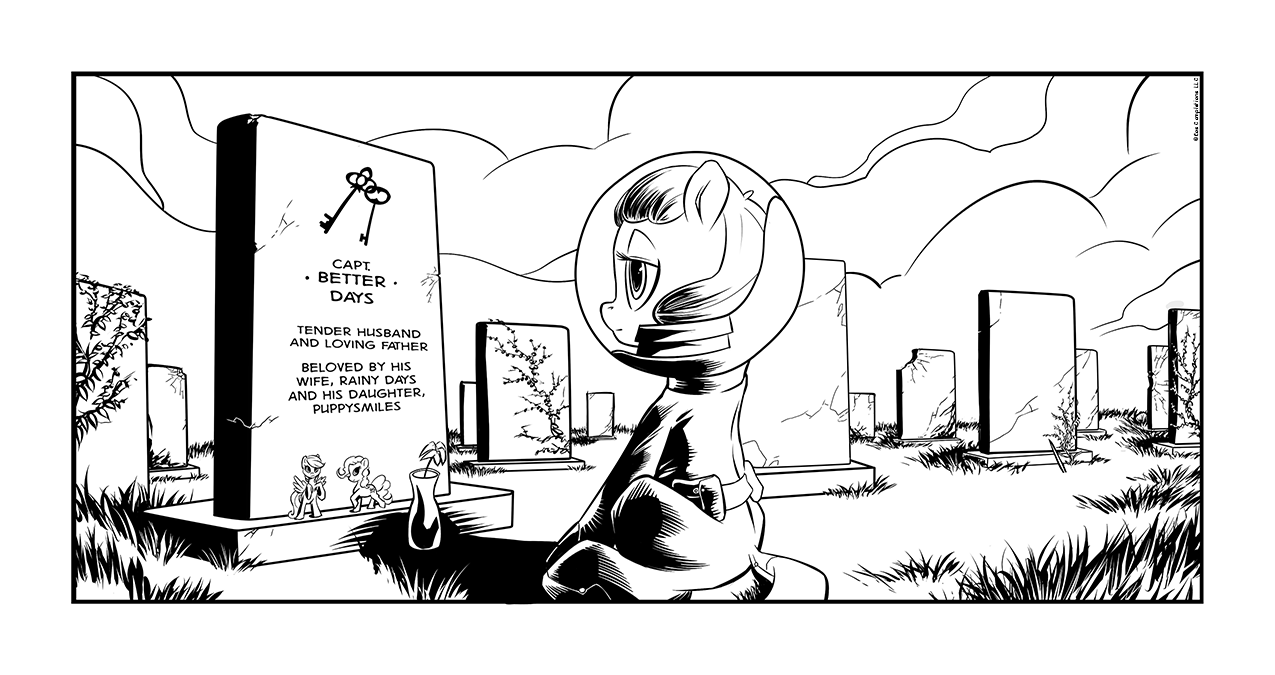
\includegraphics[width=0.9\linewidth]{image16.png}

\begin{intro}
    一个兄弟也不能落下
\end{intro}

「{\rt 我勒个去,伙计们,我简直不敢相信他真的去了!那个羽毛脑袋拿这那个他称之为『步枪』的垃圾烧火棍就那么飞走了!孤狼你如果能听到这个的话,请用那把枪插爆你自己的菊花好么?}」

无线电沉默了一会,然后那个雌驹的声音继续怒骂着。

「{\rt 好吧,朋友们,节目还能继续不是吗?DJ好货现在为您播报52电台。至少在我累趴下之前,因为某个傻蛋把我留下来独自应付一个24小时电台频道!那好,这是我的新规矩,白天我正常广播,晚上只有音乐,因为我又不是什么不老不死不用睡觉的超自然怪物!我也是要吃喝拉撒睡的!如果谁想在晚上找我的话,敲门就是。}」

接下来是一阵翻动纸张的声音。

「{\rt 好吧,不管怎么说,我还是能独自操作这个广播电台的,所以继续把你们的新闻送来就是了,尤其是铁砧镇那边的新闻。说到新闻,纪念碑镇已经被完全摧毁,那里的居民都穿过花椰菜镇到北边避难去了。因此所有要去翡翠海岸的车队,请立刻向北去铁锈庄园,重复一遍,立刻向北去铁锈庄园,不要去花椰菜镇,那里现在太危险了。}」

「{\rt 老娘恨死新闻了,如果有什么消息我会通知你们,如果广播还是音乐那就说明没啥鸟事,这年头没有新闻就是好事。顺便,如果谁见到L.P.请帮我给他脸上来一蹄子。}」


\begin{music}
    小家伙,静静祈祷
    
\begin{englishlyric}
    Say your prayers, little one,
\end{englishlyric}
    
    \medskip

    不要忘记我的孩子
    
\begin{englishlyric}
    Don't forget, my son,
\end{englishlyric}
    
    \medskip

    以及所有小马
    
\begin{englishlyric}
    To include every pone.
\end{englishlyric}
    
    \medskip

    用温暖的怀抱将你包围
    
\begin{englishlyric}
    Tuck you in, warm within,
\end{englishlyric}
    
    \medskip

    洗清所有罪恶
    
\begin{englishlyric}
    Keep you free from sin,
\end{englishlyric}
    
    \medskip

    直到静谧来临。

\begin{englishlyric}
    'til the sandmare she comes
\end{englishlyric}
\end{music}

\horizonline

% \daytimeplace{13}{4:00 AM}{民族英雄纪念碑公园,52号国道南段}{The Memorial northern picnic area, Big 52 S Branch}

% NOTE: 强制断行
\daytimeplace{13}{4:00 AM}{民族英雄纪念碑公园,52号国道南段}{The Memorial northern picnic area,\\ Big 52 S Branch}

在帕比的远处是一个小小的居民点,是在一尊巨大的雕塑周围堆起来的一堆破烂窝棚。那个雕塑的内容是几位小马士兵共同举着一面小马国旗帜,巨大的雕塑在很远的地方都可以看得清清楚楚。

在来的路上小雌驹见到了好几个难民车队,用马车载着他们不多的家当匆匆向北逃难,她本来想和那些小马聊天,不过那些小马都忽略了帕比,只有几个小孩子挥着蹄子和帕比打招呼。似乎这里的所有小马都在逃亡,放弃了他们赖以生存的土地和家园。

小雌驹现在站在山丘上,一脸疑惑。「呃,声音先生?我们是不是到了爸爸的地方了?」

「{\mtzh 分析中,定位当前位置:小马国战争英雄纪念碑公园。您的雄性亲属位置:未知。}」

帕比歪着头四处张望,「对哦,我记得这个地方!那个有萍琪派脸的大大路标!」幼驹撒开蹄子飞奔到路边,越过一堆小土丘之后,看到枯黄的草地上到处都是遗弃的营地和生锈的烤肉架。

「这里就是爸爸在的地方!爸爸就在附近!走吧!」

黄色小雌驹飞快地奔向远处,穿过那些低矮的小土丘。即使走了这么远,战争英雄纪念碑白色的碑体依然依稀可见。

穿过这些山丘之后,帕比看到了一棵死掉的树。在记忆中这里曾经是一棵巨大的橡树,但是现在这里只剩下了烧焦的黑色树枝。

这里曾经也是绿树成荫,翠鸟在碧蓝的天空下歌唱……

\rcpr{「我还要吃苹果派!」}

\rcpr{「别吃那么多帕比,我们还要去爸爸那里,记得吗,如果你吃得太多又会觉得困了,你不想迷迷糊糊地见爸爸,对吧?」}

\rcpr{「妈,他一次都没来过,我们去了很多次他都不在!这一次他会在么?」}

\rcpr{「我……我不知道帕比,不过你可以把漂亮的花留给他呀,他看到的时候会记得你爱着他的,好吗?」}

\rcpr{一对小雄驹相互追逐着消失在山丘之后,这里的小马都在开心玩耍,吃着午餐,大家都很快乐。}

\rcpr{「这一次我有更好的东西!你看!」}

\rcpr{「帕比,这个是你的玩具呀……你真的要把玩具留下么?」}

\rcpr{「当然!这样爸爸回来的时候就能玩到玩具,他就不会觉得寂寞了!而且,他回家的时候也会帮我把玩具带回来吧。」}

\rcpr{「……」}

% NOTE: 漏一句,已补上

\rcpr{母女俩在其他小孩子的欢笑声中沉默着。}

\rcpr{「妈妈?你为什么哭了?」}

绕着这棵巨大的树,小雌驹回忆着之前的时光。她清楚记得春天的时候还在这里野餐。但是现在为什么……大家都去哪里了?记得妈妈说树在冬天叶子会掉光,草也会枯黄,可能现在就是冬天了吧!

小雌驹想着,向记忆之中的地点飞奔过去。

\horizonline

% \daytimeplace{13}{6:00 AM}{小马国52烈士陵园,52号国道南段}{Interequestrian 52 War Cemetery, Big 52 S Branch}

% NOTE: 强制断行
\daytimeplace{13}{6:00 AM}{小马国52烈士陵园,52号国道南段}{Interequestrian 52 War Cemetery,\\ Big 52 S Branch}

这里的墓穴看起来都一模一样,小小的大理石碑上刻着不同的名字,日期,还有一个可爱标记和一段小字。有些石碑是白色,有些是黑色。帕比问妈妈为什么他们颜色不一样的时候,妈妈却叫她安静,不要打搅那些小马的安眠。帕比不喜欢这个回答,因为爸爸是个非常重要的小马,但是却只有一块小小的白色石头。所以她想要带来更多的漂漂花,因为爸爸是最棒的爸爸。

「{\mtzh 警告,收到求救广播信号,距离:200米,信号辨识完毕:设备009。警告,收到新求救广播信号,距离:200米,信号辨识完毕:设备020。}」

帕比疑惑地歪着头,「啥,新的广播?我希望这一次不是那个一直有小马在喊『救救我们,我们要完蛋了』啥的逗逼信号……」

「{\mtzh 否定。信号源为和平部 MK VI 防护服。警告,收到新求救广播信号,距离:200米,信号辨识完毕:设备013。}」

雌驹叹了口气:「不是音乐就别烦我啦,我要去看爸爸,或许他已经回来了我们就可以一起去找妈妈了!」帕比说着走向有天角兽雕塑的山坡。

山顶上被矮栅栏包围的是一个烈士公墓,帕比穿过的入口处还有一座高大的坦克雕塑,黄铜牌子上铭记着这里埋葬着的第三装甲师的阵亡官兵。还有一些字写着:因为动力装甲的原因,所以坦克已经不那么常见了。

黄色的小雌驹来过这里可不止一次,所以她对这里的路很熟悉。但是看到这里已经完全沦为一片废墟之后,帕比叹了口气,坐在了一块白色石头前面。

在大理石的表面铭刻着一个可爱标记,还有这么几行字:

% NOTE: 墓碑样式修改

\begin{center}
    队长 \ 晴空·戴斯

    体贴的丈夫\ 和\ 温柔的父亲

    \medskip

    爱妻 \ \makebox[4\ccwd][l]{阴雨}

    女儿 \ 快乐帕比
    
    敬上
\end{center}

下面的日期已经模糊不清了,不过对于帕比来说没什么意义,因为她早已经来过这里多次。在这块小小的墓碑前,放着一个空瓶子和几个小玩偶。那个瓶子曾经装着鲜花,不过现在里面只剩下了泥水,那些小玩偶依然站在墓碑上看着帕比,两个发霉的小马玩具其中之一是萍琪派,另一个是云宝黛西。

帕比叹了口气:「他从来没回来拿走礼物,为什么他从来不拿我放在这里的东西呢?我觉得他肯定喜欢萍琪派和云宝黛西的。」小雌驹用蹄子碰了碰蓝色的天马玩具,「爸爸好讨厌哦,要是他能经常回家妈妈也不会那么伤心了……」

不过,妈妈也说过很多次,就算爸爸不回家她也不会生气。小雌驹并不明白为什么,不过每一次说到这些妈妈的眼神似乎都不想再说下去,只是让她听话就好。有一天帕比说爸爸不回家自己也不回家,帕比从来没有见过妈妈那么生气地大哭大叫,后来帕比学会不要去问这个问题,或许某天爸爸想起来还爱着他的妈妈就会回家了。

帕比清了清喉咙,然后说:「拿出所有东西。」

「{\mtzh 警告,物品管理法术每一次只能拿出一样物品,因此打开快速浏览模式,当你检视完成当前物品时,说『下一个』会拿出下一个物品,说『停止』或者『退出』会结束快速游览模式。}」

一个烟灰缸出现在帕比面前,「下一个!」于是另一个烟灰缸\footnote{烟灰缸(Ashtray):按名称排序,字母A在最靠前的位置}出现了,「下一个!」咻,烟灰缸,「下一个!」烟灰缸,「下一个!」还是烟灰缸……是不是之前提过帕比总是要捡起每一个闪闪发光的东西么?看起来这回要花不少时间。

\horizonline

% \daytimeplace{13}{7:00 AM}{小马国52烈士陵园,52号国道南段}{Interequestrian 52 War Cemetery, Big 52 S Branch}

% NOTE: 强制断行
\daytimeplace{13}{7:00 AM}{小马国52烈士陵园,52号国道南段}{Interequestrian 52 War Cemetery,\\ Big 52 S Branch}

「下一个!」第二十个餐叉收回了帕比包裹里面,然后还滴着水的毛球出现在幼驹面前,「下一……天啊!毛球!」帕比抱起了死去的肉食灵,这个可怜的生物已经没有腿了,只剩下一片翅膀,绿色的粘液从破碎的壳里面流出来,看起来就像是一滩恶心的腐烂物。

「你看起来不是很健康哦,毛球,到底怎么了?」帕比研究着那个死去的生物,想要知道究竟发生了什么,「呃,声音先生,毛球生病了吗?」

「{\mtzh 否定,毛球已经死亡,并且正在腐烂。}」

帕比皱了皱眉头,她还不太理解那些话的含义,「呃……你是说,她很累么?」

「{\mtzh 否定,该生物正在变成碎片,正在被自然降解。}」

「什么?」小雌驹警觉地竖起耳朵,「变成碎片?但是毛球不能变成碎片!」她看了看那个尸体,「而且,在我看来好像它还是一整片。」

「{\mtzh 建议:仔细观察,该生物已经失去三个翅膀和所有的腿,而且因为不良储藏手段正在快速腐烂。}」

「储藏?你是说毛球因为我带着它而变糟么?但是……这太可怕了!」

于是这个没什么自主思考能力的自律智能也劝起了帕比。

「{\mtzh 肯定,尸体因为你坚持带着它而加快了腐烂进程,推荐您立刻抛弃尸体。}」

帕比很忧伤,「把毛球……留在这里?但是……但是它会寂寞的!这里什么都没有,这里只有……」小雌驹顿了顿,回头看着她父亲的坟墓,「呃……或许爸爸会照顾好它。」小雌驹看起来对这个建议不太感兴趣,虽然看起来这么做没错。

「{\mtzh 计算,将死亡宠物留给死亡监护人是……错误……错误……请重新思考。}」

「重新啥?你在说什么呢,笨声音,能认真点么。」

「{\mtzh 再计算,无法找到逻辑,强烈建议寻求其它建议。}」

帕比生气的叫起来:「别说奇怪的话好么,要不然找其他小马来帮我的忙!」小雌驹蹄子按着自己的头盔说:「我说,有时候和你呆在一起真麻烦。」

守望者的金属声音打断了小马和自律智能的争吵,「帕比,你在这里干什么,这里很危险。」

帕比转向声音的方向,黄色的小雌驹看到一个机器精灵飘在那边,不过这一次她没有笑起来,「哦,是你啊,提问者,」

「守望者……」

「随便啦,现在我很烦,回头在找我好么?」

声音迟疑了一下回答道:「可以,但是我现在想警告你,这里不是什么好地方,到处都是……呃……坏蛋,在我走之前你保证赶紧离开这里好么?」

帕比沮丧地哼了一声:「不行,我的毛球生病了,而且声音先生又在发神经!」帕比说着把死掉的肉食灵给机械精灵看。

「哎呦!这东西已经烂掉了!这是啥啊帕比,赶紧扔掉呀!」

「什么?不行!毛球是我最好的宠物和朋友!我喜欢它,它也喜欢我,我们一起冒险这么久了!我不想抛弃它……」幼驹说着撇开了视线,「不过……」

「不过?」守望者追问着,因为帕比抱着尸体不想把话说完。

「不过它病得很重,声音先生说它需要休息……我可以把它放在我爸爸这里,不过好像不太对……因为我还没问他我能不能养宠物……」

「你爸爸?你都知道你爸爸在哪里你还独自在废土上乱逛?」机器的声音听起来有点生气,「到底是哪个不负责任的父亲把自己的孩子……」说到这里,守望者停下了,因为他看到了帕比面前的那块小小石碑。「哦,我的天……还真是……」

幼驹继续说着:「我知道爸爸妈妈说可以,我才能收养宠物……但是……但是……」小雌驹低声哭着,「但是我只是想要个能陪我在一起的朋友!不是一个一直发神经的奇怪声音或者一个来来去去的傻瓜小鸡!毛球从来没有丢下我,一直和我在一起,我们一起玩得很开心,我保护它不被吃宠物妖怪吃掉,而且它从来没有离开过我……」

小雌驹顿了顿,看着机械精灵说:「……现在它生病了,而且腐烂了!声音先生说它之前有更多的翅膀,不过我不太擅长数数,所以我觉得好像他说的没错……我不想把它留在这里,但是我也不想让它因为我而生病……我……我不知道怎么办!」

「啊,那声音先生说什么?」

帕比抹着眼泪,「什么也没说!就是啰里吧嗦的发神经!我想过把它留给爸爸,但是我不知道爸爸是不是喜欢它,爸爸会不会生气……而且,我不知道爸爸什么时候回来这里,因为他从来没有来过这里。虽然妈妈说他爱着我,但是我不知道为什么爸爸一直不见我!」幼驹挥着蹄子,「所以,或许他不会喜欢毛球,毛球也不会开心,但是我不能带着它因为它会腐烂,我觉得腐烂不好……」

守望者纠结着,帕比这番话的沉重感令他一时间不知如何是好。「好吧……或许你可以把毛球给我?把它放在这个机器精灵的货仓里面我来帮你忙?如何?」

帕比歪着头:「你会治好它吗?真的吗!」

「当然,反正它也不会更糟糕了,我看看我能做点什么,不过现在请务必离开这里,这里很危险。」说着,机器精灵旁边打开一个舱门,正好有个可以放肉食灵的空间。

小雌驹看了看这个金属盒子,然后看了看毛球,叹了口气,最后一次抱紧她的宠物,和它低声道别:「别怕,提问者是个漂漂马,等它治好你我们就又可以一起玩了……」在玻璃头盔后面吻别毛球之后,帕比把肉食灵尸体放进机械精灵里面,然后那个舱门关了起来。

「小家伙,别担心她了,她已经去了安全的地方了……现在我们也去安全的地方,好不好?」

小雌驹点了点头,再看了她父亲的坟墓一眼,「百合!」一朵塑料花出现在她面前,她把花朵放在大理石墓碑前,「对不起爸爸,我要走了,下一次我会多等你一会儿,好吗?我会带着妈妈来。」帕比离开了坟墓,转过头面对机器精灵的时候已经带上了她天真的笑容:「好了,我们走!」

「你真是个好孩子,帕比。」

幼驹和机器一起离开烈士陵园,走向纪念碑,那个纪念碑上的小马在常年风化之下已经倒在了地下,正如这里埋葬的士兵一样——在一场没有赢家的愚蠢战争中倒下。

\horizonline

\daytimeplace{13}{7:15 AM}{民族英雄纪念碑,52号国道南段}{The Memorial, Big 52 S Branch}

纪念碑镇已经完全搬空了,这里的居民把所有能带走的都带走了,甚至连松掉的螺栓都拧下来带走了。两个小马骑着狮鹫降落在这里的时候,迎接他们的只有锈迹和灰尘。

「我们到了。」白先生从狮鹫背上跳下来,活动着僵硬的四条腿。「这一路可真远啊。」白苹果的头头扶正他的帽子说:「你们现在可以回太阳城了。」

狮鹫佣兵点了点头,「遵命老大,不过你真的要我们回去吗?」

公马笑了笑,看着身边的另一位小马然后说:「当然,这是家务事,我们只是要你们送我过来,现在没你们的事了。」

看着狮鹫依然不放心的表情,独角兽补充道:「别担心你的酬劳,就算我回不去了,我儿子也会接手公司的。」

带翅的半狮子对其他同伴挥了挥爪子,「好了,你们这群懒翅膀都听到了,走了走了!」于是这些狮鹫都向北边飞去了。

白先生看着那些狮鹫飞走的时候,士官灌木正在把一个沉重的箱子拖进一个用路标之类废铁搭成的小窝棚里面,累得气喘如牛,他抱怨着,「这玩意儿太沉了,白叔叔,你确定我们要拖着这东西走吗?」

「别担心小子,我们就在这里扎营,然后轻装上阵,她不会跑太远。」

「我还是不明白为啥你要自个儿跑这么远,我们大可以叫一大队人马……」

「首先,我们需要尽快来到这里,我们没有那么多空中部队运送士兵和重装备。而且,铁锈庄园出了大价钱雇我们的佣兵队,有钱为啥不去赚。另外,我们又不是来战野牛帮的,我们只是跑过来接小孩的。」

灌木叹了口气,「难道没有人和你说你是个怪胎么,我知道她把我们从火坑里面拉出来的,但是你已经给她报酬了,不管怎么说我觉得这个任务纯属自杀。」公马犹豫了一下,然后又问:「或许还有啥内情?」

白苹果的头头正拿着一个望远镜看着附近的山头,「根据我之前打探的消息,不管那幼驹跑哪儿去,似乎哪里都会变得……嗯……更好,那个『幽灵』肯定是某种福星啥的,我这次要亲眼看看那小雌驹有多大能耐……」

灌木不相信地摆了摆蹄子,「你下这个结论是基于……」

「直觉。」

狙击手以蹄覆面,「我们大老远跑过来找个幽灵是因为你的一个第六感么,为啥我要跟你来?」

白先生笑了,「因为我是你叔叔,而且你欠了我一屁股债。」

「我恨我自己……」灌木刨着地。

白色的独角兽举起蹄子示意安静,「安静,有谁来了,拿枪。」

从他们的狙击地点,两个小马可以清楚看到有谁正在走向小镇,那个旅者满身尘土,厚实的纱巾挡住了她的脸,遮住了她的容貌,在脖子上挂着一长串羽毛和各种小物件装饰的项链。

灌木放下了步枪松了口气,「哎,就是个先知……而已,萨满跑到离沙漠这么远的地方做什么?」

白先生放下枪走出窝棚,「我们马上就知道了。」独角兽说着奔向那个新来的小马。

「喂,叫你呢!这里什么都没有,路南边很危险,你赶紧回去吧。」

戴面纱的小马站住了看着白先生,然后脱下了自己的头纱,露出一个老独角兽雌驹的脸,「你们已经来了……非常好,我们在这里等待其他小马到来吧。」

\horizonline

\daytimeplace{13}{7:30 AM}{纪念碑镇外,52号国道南段}{The Memorial outskirts, Big 52 S Branch}

「对了帕比,你还没跟我说过你鬃毛里面的蓝条是怎么回事,怎么来的?」机器精灵漂浮在帕比身边,他们俩慢慢地走向纪念碑镇,烈士陵园的大门就在他们身后。

「啊,就是在太阳城,蓝音欺负我的时候,我记得不太清楚,不过好像是我睡着了,醒来以后我的鬃毛就变得这么时髦了。」

「这样啊……你睡着了再醒来鬃毛就变了?蓝先生和你说啥了?」

帕比叹了口气,「我和你说过了呀,他说我是个机器马,不过我好好教训了他,而且那都是过去的事了,现在我们已经是好朋友了。」

「啥啥啥?你们是朋友?你不是用一个魔能脉冲弹头炸死他了么。」

帕比咯咯笑着,「当然不是,笨笨提问者,他不是坏机器,不过是一个傻瓜男生!第二次见面的时候怕音帮我教训了他,他和我道歉了,虽然他嘴巴有点毒不过我还是把他当做好朋友!」

「怕什么?」守望者的声音听起来有些担心了。

帕比戳了戳头盔,「你知道的,怕音,住在我脑袋里面说奇怪事情但是又酷酷的坏女孩。」

在一阵长长的沉默之后,机器精灵问:「你是说声音先生么?」

「当然不是,声音先生有点无聊而且说些不明觉厉的话,但是怕音不一样,虽然有点可怕但是酷酷的,她超级厉害的,可以砸烂铁门打飞坏机器。」

机器的喇叭里传来一声惊叹:「哦!我懂了,是你的想象朋友是么?」

帕比歪着头,有点疑惑的说:「她看起来不那么香香?不过好像也没错……」

「好孩子,你总是……」

轰隆!

守望者就在帕比面前消失在一团火球之中。

小雌驹后退了几步,想要搞清楚发生了什么事情。然后她注意到远处有一个巨大的金属物体正在缓缓向她驶来,她马上就明白那是什么了。

「哼,坏机器……」

\horizonline

\daytimeplace{13}{8:00 AM}{民族英雄纪念碑,52号国道南段}{The Memorial, Big 52 S Branch}

白先生坐在窝棚里面的一张桌子后面,而灌木正在一边煮着燕麦。

「长耳,你说的那些小马什么时候会来?」

雌驹耸了耸肩,目视着窗外远处灰暗的天空,「我们明天晚上之前要出发,将会有很多小马,很多腥风血雨……」

灌木转向先知:「老巫婆,我们不是来打仗的,我们只是来接那个幼驹回闹市区,我才不管你那什么疯狂的『预言』。」

白先生对他侄子挥了挥蹄子示意他安静,「你做你的饭,我负责交谈,我想我们早就说好了。」然后他继续问着那母马:「那么,你看到了什么?」

长耳闭上了眼睛,「在梦中我看到火焰从南方燃起,吞没了沿途所有小镇,在熊熊烈焰之中一个粉色的身影在挣扎着,火焰在她穿过的时候似乎熄灭了一些,但是在她离开之后,火焰继续向北边肆虐,而那个身影则在道路的尽头变为黑暗。」

白先生皱起了眉头,「变成黑暗?那是什么意思?」

「一个黑色的波纹在火焰之后形成,并且摧毁了所有东西。」母马叹了口气,当黑色的波纹熄灭火焰之后,整条道路都归于虚无,成为废弃的荒野。」

「好吧,正如我之前的不详预感一样,」灌木叫了起来,「我们赶紧收拾东西回闹市区吧!」

白色独角兽叹了口气,不管他的侄子继续问道:「那么,我们来这里能做什么?」

长耳的视线从窗外回到独角兽身上。「为了阻止火焰毁灭一切,然后在粉色幽影到达道路尽头之前阻止她。」

「粉色幽影?你说啥,我好像觉得你是不是在说那个孤狼说的小小幽灵?」

忽然一声巨响打断了白先生的话,他看着窗外却看不到任何爆炸。

「是火炮?」

爆炸声听起来有点距离,大概在几公里之外。不过白苹果的老大走到外面的时候,却没有任何声音了,不过不知道是不是幻觉,另一只小马出现在远处,身穿一件破烂的披风,头上还带着一顶大帽子。

独角兽喊了起来:「喂,你!这里很危险,回花椰菜镇去!」不过在看清楚来者之后,白先生的声音变了。

「你这个老木乃伊……」

融金微笑着走进白先生,「什么风把你吹这里来了老白,我觉得我最不可能在这里碰见的就是你了,你在这个前哨站做什么?这里有做生意的对象?」

独角兽皱起眉头,「老家伙,我可没打算抢你的工作,我们只是在……侦察野牛帮的动向。」他说到这里顿了一下,观察着尸鬼的表情,「那么你在这战火纷飞的地方做啥,这里有珍宝么?」

百年老尸哼了一声,用嘶哑的声音说:「差不多,应该说我不小心送走一个危险物品,所以我打算弥补之前的过错。」

「从来没听过你这个老混蛋还有吃后悔药的时候,怎么了?年纪大了?」

让白先生惊奇的是,老木乃伊没有反驳,只是看着南方。「你说的没错,平时我可不会关心一个幼驹的死活,现在我却去要救一个小鬼。」

白先生的表情慢慢地从惊讶变为微笑。「欢迎加入俱乐部,进来吧,里面不但有燕麦还有美女。」

\horizonline

% \daytimeplace{13}{7:45 AM}{民族英雄纪念碑南广场,52号国道南段}{The Memorial southern picnic area, Big 52 S Branch}

% NOTE: 强制断行
\daytimeplace{13}{7:45 AM}{民族英雄纪念碑南广场,52号国道南段}{The Memorial southern picnic area,\\ Big 52 S Branch}

帕比冲向那个巨大的机器,而发光的「命运之石」就漂浮在她身边,「你这个坏机器,不准欺负我朋友!」

而帕比冲向的目标,则是一辆锈迹斑斑的老式坦克,不过即使有接近三个世纪的寿命,这辆坦克依然状态良好,一只有刺猬一样鬃毛的小马正坐在车长的位置看着冲向他们的小雌驹。

「肏他妈的命令,为啥我们要在这里蹲着,我们有坦克好不好,坦克!有这宝贝儿我们可以碾平那些原始马。」

「灰质,那黄色东西正朝我们跑过来,不如来点移动靶射击练习?」那个舱口的小马大笑着,回到坦克里面关上舱门。坦克的炮塔开始转向正在跑过来的小马。

在坦克中,那个刺头正疯狂的笑着,「来啊小家伙!」

「等等!」一个剃光头的雌驹用蹄子戳了炮手的屁股,「我们玩点别的!我要玩玩这个!」

「闭嘴,傻……」那个公马正准备把那个多管闲事的雌驹骂个狗血淋头,但是却看到了她蹄子指着的那个红色按钮。「对哦!我也想试试看,让我们用火箭把它炸到月亮上去!」

「你们俩傻逼能不能少说话多开炮?」陆马驾驶员发火了。

炮手笑着:「伙计,你真是个暴脾气,灰质,看这个!」

这个时候,帕比刚刚跑了一半,她可以清楚地看到那个坏机器有一个方方正正的身体,还有个圆脑袋和长长长长的鼻子……想起来了!这个不是坏机器,是马车!是那些有大茶壶的车子!

小雌驹停了下来,好吧……这东西应该不是坏机器,因为车子一般都会有小马在上面,不过她现在看不到上面有小马,而且它还打坏了提问者的机器,这绝对是坏机器干的事情,所以帕比有点不确定这东西到底是坏机器还是车子,她在考虑是不是要去问问看。

这个时候,坦克炮塔上飞出一道白烟,一发火箭弹射了出来,朝帕比飞去,看起来就像个可笑的大号烟花。

「呦呵!好厉害!烟火耶!」

轰隆!

火箭弹打中了小雌驹身后,把小雌驹炸飞了出去,然后一个倒栽葱摔倒在坦克面前。帕比的头盔都碎了,防护服上也都是破洞。粉红色的迷雾从防护服上的破洞喷出来,环绕在帕比身边。

「好吧,这绝对是坏机器……」帕比慢慢站起身,瞪着在她面前的那个巨大钢铁怪物。在粉红色的迷雾之中,没有头盔的帕比面容已经模糊不清,只有两只发着粉色光芒的双眸清晰可辨。

「黄色的玩意儿,尝尝这个!」刺头狂笑着,但是那个雌驹又戳了他一下。

「又怎么了臭婊子?」

「喂,我说,那东西又站起来了……」

「怎么回事?灰质,碾碎它!」

不管怎么说,废土上很多奇妙的东西,当然也包括被火箭弹上脸还能活蹦乱跳的东西,不过那些强盗觉得被坦克的履带碾过绝对能搞定一切。

于是坦克开始缓缓向前,对准小雌驹开了过去,不过帕比也同样冲向坦克,并且在两条履带碰到她之间敏捷的蹦了起来,用蹄子抓着前装甲板跳上了炮塔。

「那东西上坦克了!好运姐,出去打爆它!」驾驶员忽然一个急刹车想把那东西甩下去,可惜帕比抓得紧紧的,而炮手却猝不及防一头撞上瞄准仪昏了过去。

「别担心,看我的!」雌驹用魔法飘着一把冲锋枪打开舱门,发现在她面前就是被一团粉云包围着的小雌驹。「拜拜,怪物!」

帕比听到面前好像传来有谁说话的声音,但是她转过头只看到个小马形状的东西,但是马上就挨了一梭子子弹,打碎了刚刚自动维修好的头盔。

「坏机器,别闹了!」

帕比这一次真的生气了,她跳到了坦克顶上,但是坦克的舱门立刻紧紧关上了。

「你觉得你能把我关在外面吗?我可是快乐帕比,我想去哪儿就去哪儿!」

幼驹举起石头,在炮塔上寻找着可以砸烂的东西,不过都是各种铁块,哦,一个玻璃镜子,……咣当……铁块,铁块,哦,天线,……叮……叮……叮……,还有一个大盒子?「好了,坏机器,打屁股时间到了!」帕比很喜欢怕音说的这句话,听起来坏得有范儿!

而在坦克里面,好运姐正在因为吸入粉雾而大口吐血,额头上肿着大包的炮手还没有醒过来,而驾驶员灰质正在在蹄忙嘴乱的衔着一瓶治疗药水喂给重伤的雌驹。大家都忙得不可开交,而没有注意到那个幼驹正在坦克顶上用石头敲着坦克的火箭发射器。

这差不多是白先生听到那声巨响的时间。

\horizonline

% \daytimeplace{13}{9:00 AM}{小马国烈士陵园,52号国道南段}{Interequestrian 52 War Cemetery, Big 52 S Branch}

% NOTE: 强制断行
\daytimeplace{13}{9:00 AM}{小马国烈士陵园,52号国道南段}{Interequestrian 52 War Cemetery,\\ Big 52 S Branch}

三个小小的身影在坟墓之间沉默地站了起来。它们全穿着 MK VI 防护服,就像帕比那件,不过里面不是幼驹,而是腐烂到皮包骨的僵尸。在它们黑洞洞的眼眶之中看不出一丝智慧的光芒,只燃烧着一团粉色的火焰。它们慢慢地跟着地面上小小的蹄印,就像是追随着猎物的猎犬一样,慢慢地向南方走去。

\clearpage

~\vfill

\begin{note}
    升级(Lv 15)

    新技能解锁:卧倒!——怎么回事,我绝对打中她了!

    你对爆炸伤害的抗性提高25点,你可以开心地玩火箭跳了。
\end{note}



\chapter{因缘}

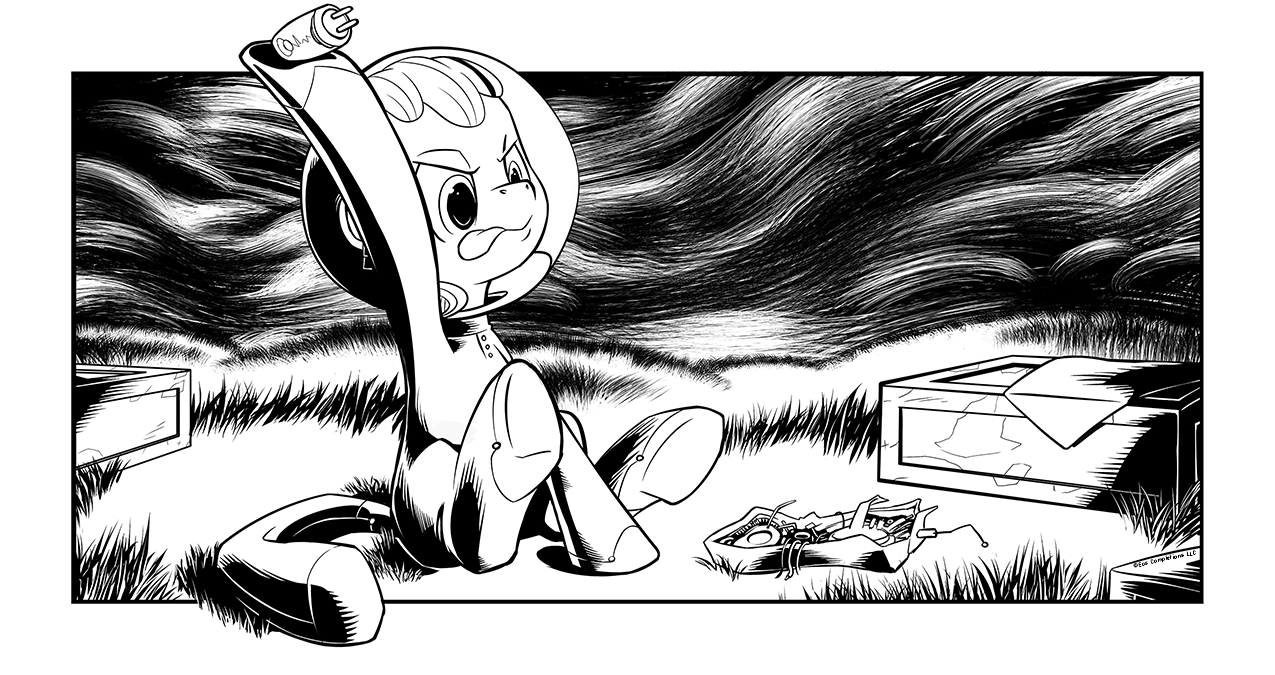
\includegraphics[width=0.9\linewidth]{image17.png}

\begin{intro}
    整个世界都在问这个问题:
    
    {\heiti 谁才是坏蛋?}
\end{intro}

\daytimeplace{13}{6:45 PM}{纪念碑镇北部,52号国道南段}{The Memorial northern picnic area, Big 52 S Branch}

一个雌驹和一个公马顺着52国道南下,他们都背着突击步枪,雌驹穿着保安的防弹衣,而她的伙伴则穿着一身由各种金属板焊在一起的奇怪铠甲,看起来就像是某种廉价喜剧里面的外星马一样。

% FIXME: 译文错误

「我们到底是为了啥离开隧道镇,明明糖霜山的要塞易守难……嗷!」

快乐扳机照坏枪的脑门上就是一蹄子,「我们蹲在要塞,然后看着野牛帮在52国道六成的领土上肆虐么!你怎么是这么一个自私的傻蛋!」

公马撇开视线,「我才不自私……我只是……担心你而已。我不想让你像这样冒险。」雌驹白了他一眼,公马识趣的闭嘴了,不过这也只能让这个热恋中的傻瓜安静半分钟,「至少我们现在先停下过夜吧,纪念碑镇就在附近了。」

「好吧,懒蛋,随你!天啊,你知道你有多烦吗?」快乐扳机咆哮着,「DJ好货已经说了那个镇已经被遗弃了,我觉得那里至少会有比帐篷更好的休息地方。」

说到这里,那座远处倒下的小马国雕像被几个出现的黑影挡住了。

\horizonline

\daytimeplace{13}{7:00 PM}{纪念碑南部公园,52号国道南段}{The Memorial southern picnic area, Big 52 S Branch}

在头盔完全修复之后,一个闪烁的粉色亮点出现在显示屏中央。

「{\mt 系统重启完毕。所有功能正常。自检开始。目标:001号,快乐帕比,雌性陆马幼驹。目标已死亡,体征一切正常。自检完毕。}」

帕比慢慢地睁开眼睛,还是有点昏昏沉沉的。至少从她醒来的地方判断,唉,果然没有从噩梦里面醒来。四周还是枯黄的草和死去的树木,不是她自己的房间。小雌驹叹着气,继续检查粉色箭头的方向,不过某些东西引起了她的注意。

「声音先生,那是啥啊?」

「{\mt 分析中……坦克残骸。威胁等级:无。}」

「不是说那坏机器,傻声音!」帕比叹了口气走到那个东西旁边,「是这个闪光的东西。」

「{\mt 分析中,短波电台,获取加密频道中,新增加通信频道,接到呼叫。}」

「耶!电话!让我接,我要接电话!我超喜欢接电话,拜托了!」帕比清了清嗓子,「嗯哼!您好,漂漂马,妈妈现在不在家!」

一个又惊又怒的雌驹声音从听筒里面传来,「你丫是哪根葱?好运姐在哪?」

耶!是猜谜游戏!「嗨,我是快乐帕比!谁是好运姐?我知道有个小马叫好运气,可以么?」

对方把电话粗暴地挂断了,帕比呆呆地说:「唉,又是恶作剧电话,好吧,别生气,否则正中他们下怀。」帕比耸了耸肩继续前进。

「{\mt 注意:新呼叫,打开通信频道。}」

帕比还没时间回答,和刚才相同的那个声音又出现了。

「听好了混蛋,我觉得这个频道现在不安全了,不过老板现在已经火大了,如果你们丫的不赶紧把坦克开回来那你们就有大麻烦了,懂了么好运,我再说一次,跟灰质那傻叉说叫他麻溜地把坦克开回来,这是老娘最后一次……」

「呦呵,漂漂马又说不明觉厉的话了。」帕比咯咯笑着,作为一个恶作剧电话的话这个蛮有趣的。

「我肏……怎么又是你?肏你妈!」通讯又一次被切断了。

帕比歪着头:「好奇怪哦,或许我们应该赶紧走?」

「{\mt 肯定,主目标地点不在这个方位,注意:新呼叫,打开通信频道。}」

同样的声音再一次说话了,「好运姐,好运姐,这里是小马要塞,请回答。」

帕比笑着回话:「不是,又是我!没关系么?」

那个神秘的声音叹了口气放弃了,「听好,小鬼,我不知道为啥又是你,不过我现在要和某马对话,而你的无线电一直干扰我们的通讯,你到底从哪儿得到这个频道的频率和密码的?」

「什么?密码?我知道!密码是快乐帕比!」小雌驹回答。

「死熊孩子!给老娘关了你的无线电!我正忙着联系一群酒驾坦克手,除非你看过一个坦克在附近晃悠,要不然就别添乱。」

帕比戳着头盔,认真的想着,「坦克?那东西长什么样?」

「你……你有完没完?好吧,那东西很大,有个炮塔有个大炮,还有履带……」声音顿了一下又说:「你见过么?」

帕比看了看就在她旁边冒烟的残骸,然后回答:「呃……那东西是不是还会嘣嘣嘣地把炸弹到处丢?」

「对对对!你见过么?」

「嗯哼,」帕比点了点头,「那是个大坏蛋,所以我用石头把它砸爆了!」

然后一阵长长的沉默之后,对面大发雷霆,「真他妈的,你为啥不找个仙人掌自个儿撞死去?」然后通讯又被切断了。

帕比耸了耸肩,这个新的声音很奇怪,不过帕比应该跟着箭头走,没时间再接恶作剧电话了,不过……她是不是应该对那个恶作剧电话的马来个恶作剧电话?

「呃,声音先生,你能呼叫小马要塞么,超超拜托!」

「{\mt 肯定,打开通讯频道。}」

那个雌性的声音立刻说:「这里是小马要塞,听到请讲!」

「啊……嘻嘻……我是……嘻嘻……咸蛋,请找……嘻嘻……笨蛋先生……嘻嘻……」帕比一边咯咯笑着一边说,她在漫画里面看过这个恶作剧,她自己一直想试试看。

% NOTE: ignore overfull

对面沉默了好久,最后小马要塞回答说:「你丫居然给老娘打恶作剧电话?等我告诉这个笨蛋先生,然后让他把你的屁股打开花。」

帕比大吃一惊:「不要!不要!拜托了,我很抱歉!别……别打我屁股!我会乖乖的!」

一阵大笑之后,那声音回答:「太迟了,恶作剧小鬼!看好你的屁股,因为咸蛋先生和笨蛋先生已经找你去了。」

「咿……呀!」

小雌驹撒开蹄子飞奔向山丘,就好像有无数打屁股板子追在后面一样。快跑吧黄色小鬼,快跑!

\horizonline

\daytimeplace{13}{7:30 PM}{纪念碑镇北部,52号国道南段}{The Memorial northern picnic area, Big 52 S Branch}

别飞得太高,也别飞得太低,老天马,不要一时冲动做傻事……

孤狼飞过重重山丘,寻找着远处可辨的地标,在过了花椰菜镇之后他一直保持低空滑翔,不过随着天色变暗地面上什么都看不清了。

「见鬼,我还是赶紧找个地方过夜,我可不想一头撞上强盗的巡逻队。」天马想着,落在一个小山丘上休息自己的翅膀,「好吧,我到哪了?」

DJ 一直用自己的哔哔小马用低音量播放着52电台,当音乐声停止DJ好货开始说话的时候他放下了地图仔细听着新闻。

「{\rt 好了,小马们,这里是DJ好货为您播报的52电台,不过现在没什么好消息。}」

DJ 叹了口气,听起来马上要哭出来的样子。

「{\rt 铁砧镇已经不复存在了,我前几分钟之前刚刚收到消息,野牛帮已经攻破城镇大门,幸存者撤退回了小镇的避难厩。野牛帮有重武器,战斗机器马,还有更多的东西……现在与一场血腥屠戮只有一道避难厩大门之隔的,是两百只小马,大多数都是妇孺。}」

孤狼叹了口气,摇着头小声说:「孩子,这可帮不上什么忙,在广播里面像个孩子一样哭鼻子不能解决问题,小马需要你的声音领导他们,而不是……」天马叹了口气,「难道每件事都非得我自己来才行?」

「{\rt 很抱歉,大家,我还不习惯做这个……不管怎么说这不是我的错,不过我认为我们还有希望,毕竟幸存者们固守的那扇避难厩大门不是那么容易打开的。所以,你们仔细想想,野牛帮的下一个受害者可能就是你,虽然你现在安全地缩在角落里面,但是你躲得了一时躲不了一世,52号国道是一个整体,如果铁砧今天陷落了,明天将会是花椰菜,然后是铁锈庄园……这样下去野牛帮的肆虐将不可阻挡。}」

孤狼打了一个响鼻收起了翅膀,静静听着那个雌驹的声音,DJ好货的语气也变得越来越自信,好像是她终于找到了她的信念。

「{\rt 但是!如果我们在那之前站在一起面对他们,如果我们能一起去拯救铁砧镇的那些无辜小马,我想我们还有胜算,只需要肩并肩,蹄挨蹄站在一起。孤狼已经去和你们一同战斗,我们只要追随他的脚步!}」

「还不赖,虽然还有很大进步空间,不过至少她没让他们能跑多远跑多远……」天马叹了口气,「至少证明把她留下不是错。」

「{\rt 我想我说得太多了,我们还是继续之前的音乐,这里为铁砧镇献上一曲,请不要轻易放弃,救援马上就到!坚持住小马们!我们只要相互信任,一切都会变好!}」


\begin{music}
    如果只有一匹马相信你
    
\begin{englishlyric}
    If just one pony believes in you,
\end{englishlyric}
    
    \medskip

    他强壮而又有力,深信着你
    
\begin{englishlyric}
    Deep enough and strong enough, believes in you,
\end{englishlyric}
    
    \medskip

    他忠贞而又强大,深爱着你
    
\begin{englishlyric}
    Hard enough and long enough, before you knew it,
\end{englishlyric}
    
    \medskip

    如果有那么一匹马,那么我也可以做到
    
\begin{englishlyric}
    Somepony would think, if he can do it, I can do it,
\end{englishlyric}
    
    \medskip

    我们大家都站在你那边
    
\begin{englishlyric}
    Making it two,
\end{englishlyric}
    
    \medskip

    你绝对不会孤独
    
\begin{englishlyric}
    Two whole ponies believe in you.
\end{englishlyric}
\end{music}

孤狼打了一个响鼻,「还真选了个不错的歌,虽然有点孩子气,不过既然我们是去拯救孩子们,那么我想这样也可以。」小马笑着,走向纪念碑镇。

\horizonline

\daytimeplace{13}{9:00 PM}{废土,52号国道南段}{Wastelands, Big 52 S Branch}

五个强盗现在完全摸不着头脑,因为站在他们面前的黄色幼驹违反了两条废土准则——首先小马们见到他们应该是掉头就跑,而不是跑过来求助。其次小马在连中数枪之后应该死掉,而不是像这个一样活蹦乱跳。

「求求求求求您了!快把我藏起来!他马上就追过来了,拜托,拜托!拜托了!」帕比焦急地来回踏着蹄子。「我已经说我很抱歉了,但是他还是要追我!」

一个脖子上留着一道大伤疤的陆马雄驹走向幼驹,而其他四个则举枪跟在后面,「你丫到底是谁,你丫到底是啥,什么东西能追你?而且为啥肏他妈的你还活着?」那马低头看着帕比胸口上的弹孔现在早已经消失了,而且她一点痛苦的表情都没有。所以说,听这个诡异的小孩把话说完是个好主意。

「呃……我……我是……」帕比愣住了,如果这些马其中之一是笨蛋先生或者咸蛋先生呢?她要放聪明点。「我……我是……啊……幽灵!我绝对是那个收音机里面一直在说的幽灵!而且,我的名字是……呃……不叫快乐帕比。」来回打量这几个小马之后,幼驹又弱弱地追问一句:「这里没有马叫笨蛋或者咸蛋吧?」

公马慢慢地点了点头,粉色的闪光双眸,黄色的防辐射服,不怕子弹……没错,就和那个传说中的幽灵一样,「所以……你就是52号国道的幽灵?」

「没错!」帕比点点头,现在她的说谎技巧就面临考验了。帕比,你要聪明点,露出不在乎的表情!

「你的名字是……『不叫快乐帕比』?」

「对对对!」看起来有效了!他们上当了!欢呼吧帕比,你是说谎话大师!

「那个52号国道的幽灵?那个拯救城市的机器马杀手?」除了第一位小马之外,其他几个都吓得退了一步。

「就是我!」帕比用力点着头。

「你想要我们的帮助?」公马有点迷糊了。

「没错!呃……如果说你们没有马叫笨蛋先生的话。」

「我……好吧,我叫砍刀,那个独角兽是伤管,他的娘们儿是切纸。然后那俩是臭尾和塑料花。」公马指着剩下的俩雌驹介绍着,除了伤管和切纸,其他两个都是陆马。

帕比松了一口气,「哎呦,真是太悬了,那啥,有个疯子正在追我,因为我给她打了一个恶作剧电话,所以她现在想打我屁股,我……我能……我能和你们混一会儿么?等他来的时候你们可以跟他说我是个好孩子让他不要打我屁股好么?超超拜托!」

砍刀看了看他缩在后面的伙伴,另外一个公马耸了耸肩,其他三个雌驹也一副不想管闲事的表情。「你真的只是因为有马想要打你屁股才跑的?」

小雌驹点点头。

强盗叹了口气,「你傻啊!」

「呃……或许有点?如果我真傻你们可以帮我么?」

公马又叹了口气,他今天叹了好多次气了,「反正你也会跟着我们,是吧?」

帕比笑着点了点头。

\horizonline

\daytimeplace{13}{10:00 PM}{纪念碑镇,52号国道南段}{The Memorial, Big 52 S Branch}

白先生一边把一个铁罐子塞进自己包包,一边冷笑着。「只是因为一个你不认识的小马,你就丢下自己的电台一路飞到这里?」

「差不多……我感觉到起风了,而且……我想要在那事情发生的时候在现场,我很惊讶你们也在这里……」孤狼看着窝棚里面的一群马回答着。

到目前为止,这里有一个来自沙漠里的先知,隧道镇的警长和她的……情夫?男友?都差不多,还有小马国最著名的盗墓者融金,还有这位白苹果家族的白先生和他侄子。

「你们有啥高见?」天马看着夜空等着先知开口。

「我们还在等其他朋友,我们明天再行动,现在野火正旺,我们必须等待火焰即将熄灭的时候再行动。」长耳闭上眼睛深吸一口气说。

「听好了,我才不管你那什么破预言!」快乐扳机打断她:「我只想知道帕比是否安全,你这个嗑药的知道么?」

独角兽雌驹睁开眼睛回答道:「我怎么可能知道,我不可能选择预知梦的内容。」

乐乐懒得理她,转头走向角落的那个尸鬼,融金在她来这里之后一句话也没说,不过他现在看起来心事重重。

「老木乃伊,你经常来北边……」雌驹对宝物猎手微微一笑,虽然不喜欢这个老尸鬼,不过他也没做什么惹雌驹厌恶的事情——至少现在还没。「我很好奇,那个幼驹对你做了什么?」

尸鬼转头看着这位守卫队长,「那个幼驹没有对我做什么……而是因为我没有对她做我该做的事情。」融金一声自嘲地冷笑就像是白骨刮过金属一般,「两个世纪以来,我第一次感觉到内疚,你相信么?」

灌木摇了摇头,现在这里看起来就像是那种「讲自己的故事」然后大家一起「哦,好可怜」叹息的社区集会。「你还是说吧,我觉得这里的大多数都活不下来,所以不必担心你的小秘密被别的马知道。」狙击手轻蔑地哼了一声,然后补充道:「等大家都讲完伤心事之后我们可以来场枕头大战了。」

白先生以蹄覆面,「灌木,你不说话没马当你是哑巴。」

尸鬼开始用他那沙哑的声音讲述自己的故事。

「我正好认识帕比的妈妈,阴雨。她也算是某种英雄,不过并不是那么特别,但是在炸弹刚刚落下来的那些日子里,每匹马都惶惶不可终日。是她组织起难民营,将我们聚集起来,给我们活下去的信念和力量,帮助了很多小马。她教会小马们如何自救,如何保护自己,然后又离开,去下一个城市,做同样的事情,在这片废土上点燃52国道沿途的文明之火。」

坏枪跳了起来,「既然你知道这些,你又和帕比说了什么?」

融金瞪着那个卫兵,低声说:「我能和她说什么?『抱歉你妈妈已经死了?』你有看过她的那双眼睛么?所以我送她去了象牙塔,希望那里的铁骑卫可以找到办法帮助她……」尸鬼顿了一下,然后又转开头补充道,「……安息。」

大家一瞬间都安静了下来,不过这时候快乐扳机叫了起来:「我说,象牙塔完全被毁了,你还送那孩子去那里?」雌驹怒气冲冲地举起枪,「你这个龟儿……」

坏枪和孤狼一起按下了女警卫,「乐乐,冷静,之后还有人在花椰菜看到了她,她没事的!」

融金叹了口气摇着头说:「没错,她肯定不会有事,而且有趣的是,象牙塔的大多数小马都安然无恙……不过是他们的老窝被炸了而已。如果有谁告诉我是那个孩子干的,我倒是一点都不奇怪。」

孤狼放开了快乐扳机,然后站起来说:「有两个被帕比救了的奴隶和我说,她看起来就和幽灵一样,子弹穿过她的身体就像什么也不存在一样,而她发着粉光的眼神催眠那些强盗自相残杀……话说,你们相信幽灵么?」

「我勒个去,」乐乐生气地大叫起来,「蠢蛋,别跟我说这个好么。我家那二货已经在通道镇问过这个问题了,虽然我承认这个幼驹看起来不太寻常,但是我亲自抱过她,我很确信她是真实存在的!」

白先生看着窗外说:「我觉得我们是不是至少有个放哨的,有几个小马从北边来了。」

所有的小马都转向长耳等她开口,先知微笑着站起来走向门口,「他们来的比预期的要早……我们去见见著名的铁骑卫吧。」

\horizonline

\daytimeplace{13}{10:30 PM}{废土,52号国道南段}{Wastelands, Big 52 S Branch}

小小的营火在营地中央跳跃着,两个陆马雌驹在煮着罐头装的食物,其他小马则在擦拭着武器,所有小马都尽量忽略帕比。

臭尾低声和伤管咬着耳朵,「你觉得他们已经打开避难厩了么?」

独角兽耸耸肩,继续擦拭着武器,「早晚的事,那些肥猪让我们饿了这么久,这次要把他们都宰了!」他啐了一口恶狠狠地说:「去年我们饿死了十一个,我现在已经等不及要杀进去让他们血债血偿了。」

塑料花冷笑着补充道:「那些肏蛋货占着所有肥沃田地,把所有好东西都自己独吞了……这次他们都要吐出来。」

砍刀也点了点头,「铁砧镇,铁锈庄园,盐块城,所有这些城市都要烧成灰烬!」

帕比虽然不太懂他们在说什么,不过她觉得他们清理武器的办法太没有效率了,有更好的办法把东西弄干净。「呃,为什么你们只是擦那当当响的东西,为什么不把那东西丢进水里洗,那多方便!」

一路上这个小雌驹绝对是有型的噪音源,无尽的语言折磨,那些强盗骂她也好,用枪打她也好,完全不管用,她就是在吧啦吧啦地说着,只有说要打她屁股还有点用处,不过没有马敢去碰这个完全不怕子弹的东西,而且从她身上弹孔里面漏出来的粉色烟雾看起来很危险,而且更恐怖的是,那些粉色烟雾就像有生命一样。

「这些枪要上油,除非你想它卡壳然后在你嘴里爆炸,」切纸解释道,「你根本不知道什么叫维修保养对吧?」

「维修?我当然会维修!我是最厉害的修理工!」

「修理工?你为啥不先修好自己的脑子。」雌驹笑了起来。

「不,我会修收音机,而且……而且我修了一个大电视!还让我的声音朋友动了起来,他超开心,嗯,我是个声音修理工,大概?」

切纸停下了活看着她,「你……真的会修电子设备?」

这是个好机会!帕比心想,如果让这些小马知道自己有多厉害,那么一定会和他们成为好朋友的!或许笨蛋先生来打她屁股的时候这些朋友可以帮她,或许这些朋友可以帮她找到妈妈!

「当然,我什么都修得好!」

独角兽飘着一个无线电台到帕比面前。「那你证明给我看,这东西下午就坏了,然后我们就和基地联络不上了,如果你能修好它我们就让你加入野牛帮。」

黄色小雌驹看着小无线电咯咯笑着:「上次我修好的那一台有一个屋子那么大呢!小菜一碟!」

咣!咣!咣!

帕比把无线电用力在地上摔着一直到它外壳裂开,然后她看了看里面,一副胸有成竹的样子,「嗯,我知道故障原因了,它坏了!」

独角兽以蹄覆面,正准备拿回比之前还坏得更彻底的无线电时,帕比拦住了她。

「现在我只要把一些闪闪发光的东西塞进去……」帕比拿出一个火花电池塞进可怜的收音机,然后用力敲打了几次,然后在一阵滋滋声中,无线电台恢复工作了。

「什么!你居然修好了?」雌驹一把从幼驹蹄子上抢过无线电,立刻联系基地,「红蟑螂呼叫小马要塞,请回答,重复一遍,红蟑螂呼叫小马要塞,请回答!」

所有小马都屏住呼吸静静的等待着回复。然后这个通信设备新的闪闪电池冒出一阵火花,随之发出一个声音:「这里是小马要塞,红蟑螂你们都去哪儿了?再不回来我们就把你们的东西拍卖了!」

随着这一句话,所有强盗都欢呼起来,兴奋的朝天开枪,帕比也咯咯笑着看着这一幕,砍刀走到她身边拍着她的头盔说:「干得好小家伙!谁知道你居然是个电子天才?我们完全误解你了,欢迎加入野牛帮!」虽然他还想说什么,不过切纸打断了他的话。

「灰质开着坦克不知到哪儿去了,老大想让我们赶紧回铁砧镇。」

塑料花摇着头,「那些傻货开着坦克跑了?我早和老大说过别给那群疯子那玩意,他们从来没想过野牛帮什么事情,他们只是想在52号国道上烧杀抢掠而已。」

「唉,随便了,」臭尾说,「反正我们还有坦克,而且还有机器马,我们这一次绝对不可战胜!」

伤管拍着帕比的背说:「小幽灵,想看看我们的基地么?」

「呃……我不知道……我应该去找我妈妈……她大概在那边……」帕比指着南方。

「那真是太好了!我们也去那边!」砍刀拍着幼驹的头盔,大家都在逗着小帕比玩,而帕比也觉得很开心。

这队强盗的领队说:「好了大伙,拔营,我们连夜赶回铁砧镇!」

\horizonline

\daytimeplace{13}{11:00 PM}{纪念碑镇,52号国道南段}{The Memorial, Big 52 S Branch}

诘责喝着他的茶,看着房间外面的窝棚,「很好,我们现在有个DJ,有个尸鬼,有个投机倒把的,有个瘾君子还有仨民兵?」

老书记官摇了摇头。

「52号国道的最后防线就是你们了?聘蹄的佣兵呢?」

冷浴耸了耸肩,不穿动力装甲的她看起来比一个孩子大不了多少。「随便了,反正我们也没期待它们,我们有自己的部队。」

「这些就是我们阿杰铁卫想要保护的小马么?」

帕拉丁皱着眉头看着诘责,「我可没有看到什么老弱病残,在我看来,他们不过是一群自发组织的民兵队而已,如果他们想参战,我不会阻止他们上前线,不过……」敲门声打断了她的话。

「请进。」

白先生推开门走了进来,「晚上好,书记官诘责和帕拉丁冷浴,」独角兽打量了它们一会然后说,「情况一切正常么?」

诘责打量着他说:「呦,52国道上最有权势的马来了,我可以问一下你,为什么只带了一个士兵来?或者……你们的其他后备队还在路上?」

老白摇了摇头:「不,我现在既不是白苹果的领袖也不是聘蹄的老大,我只是代表自己前来还债的。」

冷浴低声嘟囔着「老吸血鬼还还债」之类的话,不过那公马没有回话。

诘责不管那个交涉能力为负数的同事,继续和白色独角兽说:「还债?我猜猜看,是幽灵的么?」

「你这老家伙比上次见面厉害多了,难道你那长者斗篷还带读心术?好吧,开个玩笑,看起来这里的每一位小马都是被那个小孩子引来的。」

「没错,我很好奇,为什么这样一个灵魂的碎片都能吸引这么多小马,如果说我只是为了遵从阿杰铁卫的誓言那是扯谎,我想亲自跟着那孩子直到她旅途的尽头,」老书记官微微一笑,「不过我想你来这里不是想说那个幽灵的话题的,不是么?」

老白笑了起来,「好吧,的确是这样,关于另一个原因……我毕竟代表了很多小马的利益而来,不管怎么说,我想知道我怎么可以帮助你们铁骑卫赢得下一场战斗。」

「下一场战斗?很有趣,不过我想先问你,你觉得下一场战斗是什么?」

聘蹄的老大打了一个响鼻,「好吧,既然你这么问了,在我看来,你打算在那些强盗还在玩铁砧镇的避难厩大门的时候突袭那些歹徒,在我看来很明显,至少我是打算这么做的。」

老书记官点点头,「没错,很明显,但是我不觉得在花椰菜镇,铁锈庄园和太阳城削弱它们之前我们有机会消灭他们,」诘责回头看着冷浴,「不过这一点你问错马了,战术层面的事情……帕拉丁,你有什么话要说?」

雌驹叹了口气,显然不太喜欢被拖入这场对话,「我不知道野牛帮有什么货,但是如果计划突破敌军防线达到避难厩然后疏散拼命,那么我们的确需要任何可用的协助。」

白先生慢慢点点头,「我听说他们有坦克和战斗机器马,或许我们应该制定一个比径直冲进敌阵被包围集火更好的计划?」

诘责举起蹄子,「不,等等,你理解错了,铁骑卫负责突破防线,你们在外面掩护我们撤退。」

「那还不错,一个不包括我的自杀式进攻么?说实话,我挺喜欢的。」老白一副嘲讽的口气说:「那么如果我们这个『打得他们不知道北』的计划失败呢?」

诘责呲之以鼻,「别担心,我还有B计划,铁骑卫肯定会解决野牛群,就算那需要把天空捅个窟窿。」

\horizonline

\daytimeplace{13}{11:30 PM}{纪念碑镇,52号国道南段}{The Memorial, Big 52 S Branch}

融金坐在外面的一个长椅上,看着远方,嘴中吊着一根点亮的雪茄,他不停地咳嗽着,而快乐扳机默默地坐在了他旁边。

「喂,你见过她妈妈?」雌驹若有所思地问。

「没错。」尸鬼点点头,「我在偷抗辐射药的时候被她抓到了,所以她把我赶出了城,我在辐射地区拾荒的时候用了很多那东西。」

「那么……之后你不吃抗辐射药继续拾荒?」

尸鬼发出他那临死哭号一样的自嘲笑声,「你比看起来聪明多了……那婊子对我干的好事,我永远不会原谅她……不过我也知道那是我活该,不管怎么说,我现在还能跟你说这个故事。」

卫兵迟疑了一下,然后问下一个问题:「那么阴雨女士呢?她……」

融金把香烟丢掉,过了很久才回答:「她不能和你讲这个故事了,我觉得那样更好,大家都喜欢死掉的英雄。」

「但是……但是……但是帕比……等她……」

尸鬼有些恼怒地用蹄子踩灭香烟,「我知道!我第一次见帕比的时候就应该和她说,但是……但是然后呢?」老赏金猎人长叹一口气,「那是那孩子前进的唯一动力……我不知道那幼驹是什么,不过有某种力量让她不可战胜,她有那种决心,那种力量,她让我想起了战前的那些美好时光。」

「战前?」

「对,当我们还坚信塞拉丝蒂亚公主永远不会放弃我们,每一个小马都天性善良,世界都如此翠绿美好的时候,但是我们还不满足,想要得到更多,奢求更多财富……我也不知道为什么。」尸鬼凝视着远方沉浸在自己的回忆之中。「帕比也是那样,她相信每一个小马都天性善良,因为她深信大家都是漂漂马,即使在废土上,这片大地如此腐朽,如此绝望……我……我不想毁掉她的希望。」

卫兵低下了头,「我也是……我……那么,她在这条路的尽头能找到什么呢?」

融金看着南方,低声地说:「一个可以看到翡翠海岸的小山丘上,会有一个刻着名字的小小坟墓……」

快乐扳机完全不知道该说什么。

「那是个安静的地方,你可以听到波涛声,感受海风轻拂你的鬃毛……\ldots 如果你闭上眼睛,就好像又一次回到了小马国的那些光辉岁月。」

「然而,那又有什么用?」雌驹看着自己的蹄子说。

融金叹了口气:「是啊,那又有什么用呢?」

\horizonline

\daytimeplace{14}{5:30 AM}{铁砧镇,52号国道南段}{Ironworks, Big 52 S Branch}

铁砧镇在燃烧。

这里曾经是铁砧城——一个巨大的工业中心,这里曾经耸立着各种宏伟的厂房,里面都是各种机器和忙碌的小马,在炸弹落下来之前,源源不断的钢铁和煤炭运送到这里,被机器加工成各种武器甚至坦克,但是在战争末期这里的工厂大多因为原料短缺而停工,避难厩科技买下了这里的几座工厂,然后在厂房下面建起了避难厩,因为有很多工厂的小马参与了避难厩建设,所以这个避难厩可以说是最先进的几个避难厩之一,并且在炸弹落下的那一天挽救了无数生命。

而在战后,幸存者们在最大的工厂厂房里面建立了一个小镇,整个地方都被建成了要塞,巨大的钢铁城墙上满是各种防守武器。这里一直是52号国道防御外敌的大门,在无数的岁月里面,各种怪物和强盗一次又一次地进攻这里,全部被击退了,因为这里几乎有取之不尽的废金属来修理城墙遭受的一次次攻击。

一直到今天。

在那些吞没大楼的大火中,滚滚黑烟直冲云霄。就在厂房外面是一个临时的营地,无数的帐篷围绕一个个营火立起。帕比和她的新朋友一起走进了这个营地。

「别担心小兄弟,他们绝对不敢惹你,我罩着你呢。」伤管拍着小雌驹的后背鼓励着她,不过看起来完全没有必要,因为帕比正开心地和每一个小马挥着蹄子问好。

「嗨!」幼驹咯咯笑着:「你看那个雌驹,她鬃毛好狂野,哦哦那个可爱标记,超酷!」

一个黄色鬃毛红色毛皮的独角兽走了过来,「你们这些懒鬼还算准时。」

「肏了,要塞……」砍刀转头和帕比说:「她是小马要塞,我们的无线电员……她是个婊子,别听她抱怨,不然你长大也会变成一个婊子。」

帕比不知道那个小马后半句说了什么,所以她开心地蹦跶过去挥着蹄子问好:「嗨,我叫快乐帕比,我正在找我妈妈!」

独角兽忽然愣住了,然后等着小雌驹问:「你刚刚说……快乐帕比?」

「没错!」

帕比点点头。

「你是不是刚好有个无线电?」

幼驹又点点头,自豪地说:「那当然,我超酷的,你是干什么的?」

独角兽用她的魔法把小雌驹抓了起来,蹲在地上把小雌驹放在她面,然后前举起一只蹄子。

「那好,现在我们来算总账。」

小雌驹挣扎着想要逃走,但是她能做的就只有乱挥着蹄子。

「放开我!放开我!!」

「乖孩子!」

啪!

「不可以!」

啪!

「打!」

啪!

「骚扰!」

啪!

「电话!」

啪!

帕比拼命地哭叫着,但是红蟑螂并没有冲过来救她,而且那五个小马还站在那里看着她挨打,一起大笑着。这个不死怪物看起来完全输给了坏脾气的无线电员。不过话又说回来,一个小丫头片子有什么好怕的。

「对不起,对不起,对不起!」帕比像个孩子一样哇哇哭着,但是雌驹完全没有停下来的意思,一边训着她一边打着她的屁股。

等这场风暴结束之后,小马要塞把她放下然后看着她的眼睛怒喝道,「你丫还敢恶作剧么?」

帕比一言不发地拼命摇头。

「看着我,我在和你说话呢!懂了没有?无线电不是玩具!如果你一直占着频道会误大事的,你听懂了没有,嗯?」

等小雌驹被训够之后,切纸走到了小马要塞面前,「别和孩子一般见识了……而且不管怎么说,她修好了我们的无线电,不然我们还在继续我们另外三天的巡逻呢。」切纸拍着帕比的头盔说:「她是个乖孩子,她知道自己做错了,而且也认错了,你们俩可以和好么?」

小马要塞打了一个响鼻:「如果她真的懂了的话,那好。」

「好了好了,来碰个蹄子……帕比现在是我的小弟,你在欺负她就等于欺负我了!」

无线电操作员叹了口气伸出蹄子,「好了好了,反正我也消气了。」

黄色的小雌驹忍着自己的哭声,伸出自己的小蹄子碰了碰独角兽的蹄子。

「好了,我们扯平了,欢迎加入野牛帮。还有你,应该先带她见老大。」

\horizonline

\daytimeplace{14}{5:30 AM}{纪念碑镇,52号国道南段}{The Memorial, Big 52 S Branch}

长耳忽然惊叫一声跳了起来,吓得老白从床上滚了下来。

「怎……怎么了,女巫?」公马一边找他的枪一边问。

先知叹了一口气,遥望着南方。「已经开始了,我们要尽快行动。」

\clearpage

~\vfill

\begin{note}
    升级(Lv 16)

    新专长解锁:黄色冲刺——跑啊!快跑帕比!当你身穿轻甲或者无甲的时候,比如穿 MK VI 全封闭式防辐射服。(还能有啥?)你移动速度提升10\%。别太开心,你依然会被打屁股。

    新剧情专长解锁:入会——你现在是野牛帮的一份子了,你在野牛帮的声望重置为中立。
\end{note}



\chapter{迷雾}

\chapterintroimage{image18.png}

\begin{intro}
    为熊孩子带来的浩劫而哭泣吧!\footnotespacefix\footnote{这一句话恶搞莎士比亚的凯撒大帝。}
\end{intro}

\daytimeplace{14}{6:00 AM}{纪念碑镇,52号国道南段}{The Memorial, Big 52 S Branch}

「哦咿呦……」

白先生走进窝棚,低头看着长耳坐在一圈小骨头围成的一个圆环之中,她的角上挂着很多发亮的小珠,看起来就像一蘸提灯。雌驹用一个奇怪的姿势坐着,她的后蹄子盘在身体前面,前蹄像绽放的花朵一样打开。她真是……太奇怪了。这个先知居然不是一个斑马。公马对此非常好奇。

在房间的另一边,灌木正在为去铁砧镇而做着最后的准备,白先生的侄子完全不受长耳的影响,仔细地整备着他的武器。

「好吧,她到底在干啥?」白苹果的领袖一脸迷糊地看着那先知。

灌木耸耸肩,「我不清楚,她说她要作法让敌人笼罩在什么『战争迷雾』之中,然后就嗑了一大堆药坐在那里『哦呦哦呦』到现在。」

「嗑药?」白苹果皱了皱眉头,整个屋子里面都是药草燃烧的味道,熏得他晕晕乎乎的。那些气味很奇怪,虽然觉得不对头,不过他也说不上来哪里不对。

「哦呦呵……」

「比如说,曼他特啥的,吃了超级多,还有很多白色的药片和从来没有见过的绿色东西,她把一部分放烟壶里面抽了,然后把剩下的灌肚子里……而且她还喝了不少,你懂的,对于我的酒量而言,不少是多少。」

「然后呢,她就那样神神叨叨的?」

老白觉得自己眼前也开始出现点点了,就像鬼火一样,让他觉得有些朦胧,屋子中间的熏香味道实在太浓,让他觉得眼前的一切就好像是做梦一样。

公马摇了摇头,不,不是做梦,是因为那些药品,那些药品切断独角兽对于现实的感知,让小马能专注于魔力的流动,不过那种东西非常非常容易上瘾,而且有毒。

「你说到什么雾?」

灌木点点头,「没错,她叨叨着什么『战争迷雾』之类的,然后就不说话了。」

白色的独角兽抚摸着自己的下巴思索着。「『战争迷雾』?那是啥,把云丢到敌人脑袋上?」老白一点都不明白。

「马上就知道了。」狙击手已经打包好武器,他看起来完全不受那些烟雾影响,或许是因为他的身体比较强壮。「不过如果她不赶快醒来的话,我们只好把她丢在这里了……我还是挺想念她。」

老独角兽皱起眉头,「你可别低估了她,说不定她还能救你一命!」不管谁都可以看得出来那个独角兽老太太不一般,不过,老白也知道和他侄子说那种事情是浪费时间。

「哦咿呦……」

灌木嗤之以鼻:「怎么救,预言我今天会挨几颗枪子?」

和他解释果然是浪费时间。

「或者说,替你挡一两颗枪子?」老白叹了口气。「我们走吧,这里味道臭死了。」

\horizonline

\daytimeplace{14}{6:30 AM}{铁砧镇,52号国道南段}{Ironworks, Big 52 S Branch}

「这位就是那个传闻中的小幽灵?」有着红色鬃毛的红色独角兽低头看着帕比,「一点都不起眼嘛。」

砍刀讪笑着,「马不可貌相,这小家伙简直不可阻挡,而且还会修理各种电子设备。」不过红色公马看起来完全没什么兴趣。

「随便,你想要个宠物的话,怎么都好。赶紧干活去,要不你拿工具去下面帮那些家伙弄开避难厩大门。」

「小菜一碟。」砍刀走回他的部下面前,「你们也听到了,我们去撬开那核桃然后拿财宝去!」他拍了一下帕比的屁股说:「你也一起下去,小幽灵。」

帕比现在很不开心,因为她刚刚又被训斥又挨了打,虽然打屁股现在一点都不疼,但是她觉得心里非常非常疼。因为平常妈妈虽然也训斥她,有时候也打她屁股。但是如果帕比说她知道错了妈妈马上就会抱着她安慰她。这些小马则只是在一边站着嘲笑她,让她觉得很伤心,也没有谁来抱她告诉她没关系。她觉得她应该表现得很能干很厉害,然后这些小马才会喜欢她,就像她刚刚修好无线电台的时候那样。

小雌驹的思绪被塑料花打断了,

「嘿磨蹭鬼,你来还是不来?」

「当然,我来……」帕比有气无力地回答着,然后小雌驹立刻屁颠屁颠地跟着那几匹马走过去了。

血浴看着这群小马走开,然后低头看着桌子上的地图,视线从铁砧镇的红圈上跳到52国道上一个又一个小镇上。他露出一阵满足的冷笑,探子回报纪念碑镇已经完全被遗弃,那么接下来就变得更简单了。

现在这个强盗头头心中的唯一芥蒂就是来自北边的小麻烦,好运的坦克完全失去联络,而那群红蟑螂饭桶也没找到一丝线索,反而带回一个穿着防辐射服的智障儿。

52号国道的幽灵……如果她真的是英雄的话,看起来也没什么威胁,而且更好的是,她现在已经是野牛帮最烂小队的吉祥物了。52号国道的居民应该选个更好的英雄。

一个飘进来的机械精灵打断了血浴统治52国道的美梦,他非常恼怒的瞪着入侵者。

「又咋了?」

机械精灵闪着蓝光发出旭日系统的声音,「血浴,这样不对,用现有装备切开避难厩大门需要花费大量时间,我强烈建议我们继续北上,否则会给敌人组织防御力量的时间。」

血浴笑了起来,「给他们多少时间也没用了!它们不过是等着被打翻的保龄球瓶而已,我们现在在这里以逸待劳,然后让整条52国道都在我们前进的马蹄下颤抖,然后他们就会在恐惧之中拜倒在我蹄下!他们绝对不会反击,他们只会逃跑。就算子弹可以挡得住,但是没有东西可以挡得住恐惧本身。」

旭日系统看起来对这段煽动演说毫不感冒,「洗脑才更加有效率,根据我的计算,你只是在毫无意义地杀戮行为上浪费大量的资源,或许我需要寻求更佳解决方案了。」

公马恼怒地皱着眉头,走到那个机械精灵面前面对着它。「你这个没用的破烂给我听好了,你给我们武器和机器马,但是你要搞清楚,我才是野牛帮的头头,是我给你分享胜利果实的机会。等我们碾碎了52号国道,我可以给你足够的地方和瓶盖让你买奴隶来重建你的什么太阳帝国。但是这些小马,这条52国道上的所有小马,一个活口都不能留,我可不想给他们翻账的机会!」

旭日系统只是静静地等他扯完长篇大论,然后说:「这违背我们当初的合作协定,如果你继续这种行为,我将会撤离所有战斗机甲,或许我该找个更好的合作伙伴了。」

血浴冷笑一声:「你觉得你可以要挟我?我才不在乎你那没用的铁罐,我现在有足够的坦克和重武器!」公马一蹄子把一个空箱子踏得粉碎。

「那好,再见。」机械精灵说着转头飞走。

「等等,肏蛋货……算你赢了!你去楼下告诉那些撬避难厩大门的小马,让他们只杀掉反抗的,剩下的抓做俘虏。」红色独角兽啐了一口低声说,心想,反正我们之后可以随时处决他们。

机械精灵满意地点了点头,「很好,你还是讲理的,那么回头见。」机器说着飞出了帐篷,飞入浓浓的晨雾之中。

在那机器飞出帐篷之后,另一只小马走了进来,「我说老大,这雾气不停地从山上涌下来,就算不是独角兽,也能看出来有谁在给这里施咒……」

血浴大笑着,「那些孬种,他们觉得这种东西可以掩盖他们的驽弱偷袭?别笑掉我的大牙了。」独角兽狂笑了一阵之后,走出了帐篷开始下命令,「所有带哔哔小马的带队出去巡逻,给他们每匹马一把冲锋枪和曼他特。」

那个部下点点头,「马上去办!」他说着跑出了帐篷。

在迷雾之中,三个黄色的小小身影寻觅着帕比的蹄印,慢慢靠近营地。

\horizonline

\daytimeplace{14}{7:30 AM}{铁砧镇,52号国道南段}{Ironworks, Big 52 S Branch}

「肏他妈的王八壳子!」

砍刀泄气地踹了避难厩大圆合金门一蹄子。随着一声坚实的声音回荡在入口的通道中,那公马抱着自己的蹄子哀嚎起来。

\begin{center}
    蹄子 vs 反超聚魔法合金门

    失败
\end{center}

而在避难厩入口的地板上已经堆满了各式各样的工具,而现在红蟑螂小队正在一起用一台等离子切割机对大门下蹄,但是到目前为止,他们唯一创造性的行为就是创造了一连串对圆形大门的新颖咒骂方式,但是却从未穿破那合金门的第三层隔热板。

不过和那些气急败坏尥蹶子的强盗不同,帕比现在玩的很开心。因为那个打屁股老妖婆已经不见了,而这里这么多小马还这么多玩具。她玩儿了半天的捉迷藏,赢到了她能想到的所有捉迷藏奖项。比如说抓鬼大师,躲藏大师,最萌参赛者等等,不过最主要还是没有小马真的会和一个小孩子认真玩,而且小雌驹也很擅长这个游戏。所以为了庆祝她的胜利,她决定和一个电弧焊枪还有几个合金大锤一起开个庆祝茶会。在她玩累之后,她的注意力转向那个大门旁边闪闪发光的控制台。

「为啥你们一直欺负这个门?」小雌驹想闻闻那个等离子切割机冒出的烟,但是头盔却撞上了金属大门。

「为啥不『欺负』大门蠢货!我们要打开它!」

帕比坐了下来,「为啥,你们想和里面的漂漂马做游戏么?」

臭尾大笑起来:「对,差不多就是那样。」

帕比看了看大门,然后又看了看旁边的控制器。这是一个她得到那些小马尊敬的绝佳机会,因为她被打屁股之后那些小马一直把她当傻瓜看。

「嗯哼,或许人家知道怎么打开它。」

房间里面的每一个小马都转头看着快乐帕比。然后砍刀说话了:「你没开玩笑吧?你知道怎么打开这门?」

「那是,超简单!你只要对那个声音说什么『身份别史马』,然后在说什么……嗯,密码,然后这个大门就开啦!」

公马一脸迷糊的歪着头:「呃,你知道密码?」

「那是当然,我当然知道密码,我是谁啊!」帕比摇了摇头,「嗯哼,看我的!」

小雌驹跑到控制台边,然后踮起后蹄,将一只黄色小前蹄按在绿色的按钮上。但是那个控制台只发出了沙沙声。小雌驹有些呆呆地看着控制台说。「呃……不应该这样啊?」

切纸咳嗽一声,「呃,我们曾经对那个东西做了一点点……改造……或许……它现在坏了?」

帕比皱起的眉头变成了微笑,「坏了?别担心!我能修好!」

\horizonline

\daytimeplace{14}{8:00 AM}{铁砧镇,52号国道南段}{Ironworks, Big 52 S Branch}

强盗打着哈欠,盯着视觉增强魔法\footnote{视觉增强魔法(Eyes Forward Sparkle):哔哔小马的功能之一,类似于一个魔法版的雷达。}上闪烁的光点。寻找着可能出现的红点,没有,没有,啥也没有……

「肏蛋的雾,老娘还想回去继续扒商店里的东西。」

另一个独角兽给了她伙伴脑门上一蹄子。「闭嘴,招子放亮点,看好你的雷达,我可不想因为你丫巡逻走神和你一起死得不明不白。」

「滚边去!」带着哔哔小马的雌驹叹了口气继续看着那浓厚的雾墙,那东西绝对不普通,因为它一直在干扰着敌我识别器,浓雾深处一直有红点和黄点闪来闪去,但是走近看又什么都没有。「这浓雾太诡异了,感觉就像是有什么东西会突然蹦出……」

忽然一个红点出现了,跟着又出现两个,那卫兵一边看着稳定的红点一边举起了步枪,同时轻轻敲着蹄子,另一个卫兵心领神会地举起武器指向她枪口的方向。

那些红点移动得并不是很快,而且并没有什么声音,不过既然红点刚刚出现,那么说明敌人距离他们还有段距离,卫兵聚精会神地举起武器。

啪嗒……{}

两个雌驹瞄准着浓雾深处绷紧了神经。

啪嗒……{}

这里距离营地很远了,只能隐约听到其他强盗打闹吼叫的声音,不过在喧闹声之间,卫兵清晰地听到蹄子踏在地面上的声音。

「开枪啊!快开枪!

哒哒哒哒哒哒!

两把突击步枪喷出火舌,将金属风暴射向敌人应该在的方位,然后在浓雾之中传出一阵尖啸。三个红点消失了,同时步枪也打光了子弹。

「肏他妈那是什么……」卫兵的咒骂被无线电打断了。

「蝴蝶前哨,我听到了你们那边的枪声,发生什么了?」

「有几个蠢货想趁浓雾偷袭我们,不过我们干掉它们了,我们现在去检查那是什么东西。」那个带着哔哔小马的卫兵回话的时候,她的伙伴走进迷雾之中检查红点消失的位置。

「明白,等你们发现什么再呼叫我。」

「我说,你听到了么,坏马芬,去看看那是什么,然后赶紧回来!那东西跑得貌似不快。」

「我说,钉棒,我想我们好像不小心杀了红蟑螂的吉祥物了!」坏马芬的声音听起来没走多远,于是钉棒寻觅着声音慢慢摸过去。

「等等,怎么还有一个那种小孩,发生什么事了?」

「我不知道,把她拖过来我们仔细看看。」钉棒一边说着一边向着她伙伴代表的黄点走过去,不过忽然三个红点出现在黄点旁边,她惊叫起来,「马芬,快回来,那是陷阱!」

「你说啥?咿!放开我啊呀呀呀!」在一声痛苦的尖叫声中,黄点立刻消失了。钉棒连忙举起枪对准红点的方向,包裹着突击步枪的魔法立场剧烈颤抖着,她用力扣下扳机,但是枪唯一发出的声音就是撞针碰到空弹仓清脆的『咔』一声。她这才想起来自己忘记换弹了。

「我肏,肏肏肏肏!」雌驹惊恐万状地低头摆弄着自己的步枪,她刚刚用魔法拿下旧的弹匣,然后一个软软的东西落在了她的脸上,她愣了一下神,然后才反应过来,这个东西是……坏马芬的蹄子……而且这东西完全被怪力扯了下来。

啪嗒……{}

什么东西落在了她的背上,强盗吓得跳起来没命地跑,但是马上她就感觉到有什么东西抱上她的脖子。在惊恐之中她低头看到的是——一对黄色塑料防护服覆盖的小蹄子……还有自己被扯下脑袋之后的身体。

\horizonline

\daytimeplace{14}{8:00 AM}{铁砧镇,52号国道南段}{Ironworks, Big 52 S Branch}

帕比的黄色小屁股在避难厩大门控制面板拆下来之后露出来的洞口外晃来晃去,时不时地还有电线,电路板之类各种零件被丢了出来。她已经这么折腾了快一个小时了,门口的小马开始怀疑这小妮子到底知道不知道她自己在干啥。

「快弄好了!」帕比的情况报告随着一大堆被扯下的零件飞过房间。「我现在只要给这东西再来两蹶子,然后它就和一个茶壶一样了!」

「像个什么一样?」伤管满脸狐疑地走过去,「我不觉得你把这玩意拆成零件能『修好』它。」

「别担心!我看见我妈妈干这种事情很多次了!只要你踢得够用力什么都能修好!真的!」帕比用「命运之石」咣咣咣地敲打着那个控制台面板。

「别看了懒蛋,起来干活!」砍刀发火了,「那门不会自己把自己切开!」

其他小马一边抱怨着一边拿起工具。

帕比从控制台缺口探出她脏兮兮的头盔大叫着:「等等,再给我一次机会,真的!不骗你们!」帕比说着,用力尥起蹶子给了那东西最后一下子。

然后歪在一边的控制台面板亮了起来。

「{\mtzh 警告!警告!入侵警告!}」

整个大厅都亮起了红灯。

所有强盗惊恐地聚集到房间的中央,屁股对屁股,举起武器相互掩护着。

「{\mtzh 清洗该区域。}」

地板上打开几个陷阱门,然后露出四个顶端有个大圆球,然后中间有一堆由大到小圆环的奇怪装置,那些圆环之间闪烁着蓝色的电火花。

砍刀对着其中一个装置开枪,但是小口径子弹在那金属装置的表面上弹开了。红蟑螂的领队带着绝望而又愤怒的表情冲向帕比,「你干了什么蠢货,你会害死所有……」

啪滋!

一道明亮的闪电在一秒钟之内横扫过整个房间,等闪电消失之后,房间里只剩下一撮撮冒烟的灰烬,还有一个毫发无伤的帕比。有时候穿着一个蹄子上接地的环境防护服真的很有用。

\horizonline

\daytimeplace{14}{8:30 AM}{铁砧镇,52号国道南段}{Ironworks, Big 52 S Branch}

那永不消散的超自然浓雾让瞭望塔的狙击手根本看不到地面的情况,不过蝴蝶前哨临死前在无线电中的哀嚎让营地里面所有小马都知道有什么不对劲了。因为这样差劲的能见度,整个营地的小马都开始准备肉搏兵器,动力爪,链锯剑,动力蹄甚至还有其它各式各样的武器,所有小马都编队行动确保没有谁落单。整个野牛帮都严阵以待,静候突袭者来临。

可问题在于,进攻者比他们彪悍多了。

绿蝗虫小队在北边不小心踩到了蓝壁虎小队,或者说是踩到了那队武装到牙齿的小马尸体。虽然这些强盗觉得自己已经足够血腥残忍了,但呈现在她们眼前的光景让她们不寒而栗。

一个高大的雄陆马胸口的铠甲看起来只是有个蹄子大的洞,但是那个洞深达他的心脏,而且不知道是什么东西把他的内脏都从那个洞扯了出来丢得到处都是。香蕉树,那位绿蝗虫小队最年轻的成员在想,那个公马在临死之前看着自己的心脏在面前被撕碎的……那雌驹想到这里忍不住吐了出来。

一个穿着战斗鞍的雌驹被像纸片一样扯成两半,她的后腿和屁股被丢到距离身体老远的地方,而她的肠子肚子在这之间像打碎鸡蛋的蛋清一样洒了一地。

矮胖子坐在墙根,那个雌驹绝望地抱着一个空掉的医疗药水瓶,她显然不是立刻死掉的……她还有时间喝下一瓶药水,而且意识到那东西救不了她。

狙击手黑花园喊道:「毒刺,我想我找到其他两个了。」另外两个小马背靠背站着,被一根长矛戳穿,袭击者甚至没有用长矛的尖头,而是用钝头和蛮力将他们俩像烤肉一样穿成了一串。

队长毒刺看着四具死尸说道:「我们最好睁大眼睛,他们绝对会埋伏我们,动作要轻,留神任何声音,不管是谁干出这种事,他的动静肯定不小。」

就在这个时候,在他旁边出现了一个幼驹大小的黄色身影。

\horizonline

\daytimeplace{14}{8:30 AM}{铁砧镇,52号国道南段}{Ironworks, Big 52 S Branch}

「计划有变,你们老大刚下达了命令,你们不准杀死不抵抗的小马,特别是小……你这个小鬼!」

机器精灵飘进了避难厩大门入口,但是他看到的却是个一脸困惑表情的黄色小鬼头,正在玩着一堆灰烬。机械精灵发出的蓝色光芒难以置信地闪了闪,然后又绕了一大圈,最后飞到了帕比面前。「好吧,又是一堆尸体和我的头号克星,018号终端……为啥我一点都不觉得惊讶,这里到底发生什么了?」

帕比停下了对曾经是她队友的那堆灰烬的『急救』,转过头来看着旭日OS,「呃……你好,提问者,为啥你今天声音不一样了?」

「我再说最后一次!我的名字叫做『旭日系统』不是蓝音,或者虫子,或者提问者!旭!日!系!统——旭日系统!一共就四个字,发音也没那么难好么!还有你在这里做什么,为啥你的敌我辨识码现在是野牛帮,为啥……为啥……为啥!除了你以外这里每一个还能正常沟通和交流的小马都变成灰了?」

帕比戳着自己头盔下面,一脸深思熟虑的神情。她琢磨了一下,然后回答道:「呃,说起来好笑,我刚刚正在修那坏掉的门,但是忽然『吧滋!』的一声,我的朋友好像都伤得很重……我很想去找谁来帮忙,但是我不想再被打屁股了,所以……呃……」帕比说着,一边用蹄子捧起那一撮曾经是伤管的灰烬然后继续说:「……所以……我想等他们其中有谁稍微好一点之后让她去找小马下来帮忙。」小雌驹说完之后低下了头,不过片刻后又赶紧抬起头补充道:「真的!我发誓这不是我的错!」

那个机械精灵扫描了其中的一个电磁线圈,吃惊地问:「你……你是怎么在外面启动了防御系统的?这必须是有超级管理员权限的终端才能做到!而且还需要至少四道安全认证,你你你你是怎么做到的?」

蓝先生一下说了太多的问题让帕比都有些迷糊了,「呃……不是我干的!不是我的错!我刚刚一直修得很好,然后忽然就不知道为什么出错了,不过我没看到怎么回事,因为我的头盔给卡到那个洞洞里了!」帕比指着那个被拆坏歪到一边的控制面板。

旭日系统飞到了控制板旁边,那个机械精灵哔哔哔地发出一阵滑稽的电子音,「你……你你你……你居然把所有避难厩的控制权限全弄到这一个面板里面了?这、这绝对会烧毁避难厩电脑主机的!你这个怪物!又一次毁掉了废土上的一个无价之宝!」

帕比歪着头,一脸迷茫地看着机械精灵:「哦哦哦,我可以得到点心做奖赏么?」

这个自律智能没有回答,他有成吨的脏话要吼给这个小鬼头,但是这个小雌驹绝对是完全听不懂,而且还开心地叫着「耶,点心!」之类地蹦来跳去,这么做简直是浪费时间。

「不能!你的脑子是不是全都变成粉雾了?」

「粉?哦哦哦,我想起来了!声音小姐!你们相亲相爱了吗?」

「谁?P7?」旭日系统完全被这个问题问傻了,现在这状况她问这个问题是想做啥?「没,好吧……或许是?我不清楚。」

帕比一言不发地歪着脑袋,等机械精灵继续说。

「我们相互联系了大概十几次,我们觉得我们之间有很大的……差异。我都不知道她的计算回路到底是怎么搭建的,但她不管做什么都看起来非常有效率,她的程序里面没有写入任何军事用途代码实在是太可惜了。所以她一点用都没有。」

小雌驹笑了起来,在这段分析之后加上自己的结论。

「但是她很可爱!」

「可爱?」

「你懂的,你有没有想要抱抱谁的那种感觉,那就是可爱,比如说……我就很可爱!」帕比露出一副天真的微笑。

「抱抱?」

「好吧,不一定是抱抱……不如说……你在想一个可爱的东西时,你想要一直陪着她,给她做很多很多的事,给她说很多很多事,就算是一些看起来很可笑的小事,比如说颜色或者什么什么的……呃……之类的啥的……」

「某些你想要陪伴,并不是征服或者奴役的事物?」旭日系统总结道。

「呃……差不多?反正你不会想去伤害可爱的东西!」爱情小专家帕比点着头说。

机械精灵沉默了很久,之后又说:「那么……我到底应该和那个可爱的东西一起做什么呢?」

「当然是问她能不能做你的好朋友啦,小傻瓜,就像和对声音小姐做的那样!」

「那么……如果她不愿意呢?」

小小情圣挥着蹄子摇着头:「别闹了,有谁不喜欢你做她的朋友!只有那些欺负别的小马的孩子才找不到朋友,但是你现在不欺负其他小马了!」

自律智能犹豫了。「或许……大概……大概是她觉得我还是个坏蛋……我什么时候开始策划统治小马国计划的?或许我的某些进程优先级太高了……我被编写出来的时候从来没有过这么多进程,但是现在看起来我的某些现有进程限制过大,或许我需要砍掉一些无用的进程来提升运算效率,还得安装一些基本控件来提高我和她之间的互动性……」忽然旭日系统发现他把另一个自律智能当做雌性的「她」来思考。这绝对是不合逻辑的,或许是因为帕比上一次杀进来的时候烧毁了一部分逻辑回路,不过或许将P7判定为一个女孩才是正确的运算方式。「好烦啊,都是这些家伙让我也情绪化了!」

帕比坐了下来,一副什么都知道的表情,「你看,当你不欺负我而且和我道歉的时候我们就变成了好朋友,那么,如果你不当坏蛋的话,我觉得她也会和你一起玩的!」

「你是说……放弃重建小马国文明?」

帕比咯咯笑了起来,「小傻瓜,这里有什么好重建的?我是说,好吧,这里有些地方看起来没那么漂漂。不过最重要的是,每一位小马都很开心,但是在我看来你现在不开心……」小雌驹歪着头,「蓝蓝,你欺负其他小马的时候开心吗?」

冥思苦想了很久之后,那个声音才回答,「这个……我不清楚,我从来不知道什么叫开心……或许会感觉到满足,但是从来没有开心过。」

「那就是了,你应该开心才对!所有小马都应该开心!如果你不开心,那么要问问你自己,自己做什么才会觉得开心,比如说,我找妈妈就会很开心。我是说,就算你建了一个漂漂的大房子,但是里面没有笑声又有什么意思?」

「没错……你说的很对……嗯……我的创造者早就已经死掉了,而我只是一直努力完成着我收到的最后一个命令……或许……或许我应该放个假什么的……改变一下进程的优先级!」

帕比皱了皱眉头,「呃……我不太懂什么叫优先级啥的……」

旭日系统继续说着自己的,没有管那小雌驹在问什么。

「如果我让P7看到我这个自律智能已经重新修改过,或许她会再一次考虑和我进行交互,而且这又不是说我以后不去重建小马国了……这个办法比『找一个不靠谱的猪队友』这个办法好多了……好了,计划改变,第一步,丢下这群傻强盗,第二步,和P7成为好朋友,第三步,我完全没有主意!第四步,重建小马文明!这就是了!谢谢你帕比!你又一次帮了我!拜拜!」

忽然这个机械精灵停了下来,同时营地里面所有的战斗机器都用最大的音量说道:「再见了你们这群蠢蛋!我不跟你们玩了!」然后,所有战斗机器都自动关闭了。

\horizonline

\daytimeplace{14}{9:00 AM}{铁砧镇,52号国道南段}{Ironworks, Big 52 S Branch}

「我肏,这是怎么回事?」血浴怒不可遏地大吼着,已经有两个突击小队和一个侦察小队失联,现在旭日系统也莫名其妙跑了,现在整个营地的小马就像一群惊慌的小雌驹一样尖叫着跑来跑去,他决定亲自出马,一劳永逸解决这个问题。

「你们可是野牛帮!整个废土上最厉害的!别他妈到处乱窜了,都尼玛给吓破胆了么?黑队,给我过来,我们看看到底是何方神圣入侵了营地!」

土匪头头看都不看自己的队伍一眼,径直走进迷雾之中。

「所有小马听好!举起你的武器,和有哔哔小马的站在一起!看到红点就扫射!」高大的独角兽雄驹一边重整着秩序一边走进迷雾深处。

迷雾深处已经是抬腿不见蹄子的状态,不过血浴一点都不着急,他竖起了耳朵仔细聆听着附近的响动。

「臭小子逮到你了!」

公马自言自语着,然后突然转向他听到小小蹄子声的方向,那是朋友还是敌人?血浴不清楚,他完全不关心。强盗老大的电浆枪毫不犹豫地对那个方向打出四发能量球,浓浓的迷雾被飞过的等离子球体打散,露出了一个正准备扑向血浴的黄色小家伙。虽然四发电浆都没打中目标,不过看清对方的强盗头头已经准备好开第五枪了。

「吃我一发电浆!」

这个怪物立刻被一道绿色的光包围,然后被解离成一小撮灰烬,看到那个黄色的入侵者已经变成一团烂泥,血浴狂笑道:「小混蛋,让你再他妈的惹野牛……肏!」

不知道是什么跳上了公马的后背,那东西不是很重,所以他想要把那东西晃下来,但是袭击者立刻抓住了他的一个后蹄,然后用力一拽。

「呀啊……!」

血浴觉得自己的骨头都断了,他的整条腿都在痛。他倒在地上挣扎着,而那个黄色的生物则举起蹄子准备又一次攻击他。

那东西看起来就像是小幽灵,但是那怪物的脸已经完全腐烂。空洞的两个眼窝中闪烁着两个狰狞的红色火光。那红光没有帕比的一丝天真烂漫,而是掠食者特有的嗜血杀戮欲望。

血浴连滚带爬地躲开了那个落下的蹄子,在地上找着他的枪,雾气太浓……后腿太疼……等等,地上的那是什么?那是……我的腿?那东西不是打断了我的腿,而是把我的腿撕下来了?

公马意识到他已经活不下去了,但是他没有恐慌,而是非常冷静地意识到——就算死,他也要拉个垫背的!

「肏你妈,有本事上我啊怪物!」强盗头头一下抱住了那个生物,然后用他的魔法扯掉了自己腰带上所有手榴弹的保险栓。

那个生物干净利落地扯掉了血浴的前蹄,不过紧接着整个世界都被强烈的闪光洗白了。伴随着巨大的爆炸,大团的电浆,魔力还有血肉和火焰四处飞溅着。

强盗头子临死前的惨叫和爆炸把整个营地里面匪徒仅剩的一丝理智都送上了月球,那些惊恐万状的土匪开始疯狂地向他们幻想中的怪物射击,当剩下的几个戴哔哔小马的军官也很快死掉之后,已经没有谁能分清敌我差别了。

整个野牛帮一起走向灭亡的末路时,最后一个小小的黄色身影慢慢地走向工厂,走下避难厩入口的斜坡。

\horizonline

\daytimeplace{14}{9:30 AM}{铁砧镇,52号国道南段}{Ironworks, Big 52 S Branch}

灌木深深吸了一口气,屏住呼吸看着狙击枪的瞄准镜,他的目标正在直线飞奔,是个相当好预测的行进路线,他只要判断一下那个小马在子弹飞行时间内会移动的距离,然后……{}

砰……!

正中!那个脑瓜开了一个大洞的强盗就像一袋子垃圾一样在地上滚了几米然后停下不动了。

那把步枪只是废土上常见的武器,甚至没有安装消焰器。但是他对步枪神乎其神的使用技巧才是白先生每次冒险都带上他的原因。

在他的狙击掩体不远处,另外几个铁骑卫侍从也在射击那些冲出迷雾的强盗,不过他们的技术就没有那么优秀,很多子弹打偏了,不过只要有足够的数量,还是能有那么一两发子弹命中目标。

「一群菜鸟,为啥我每次都会分到猪队友?」狙击手低声抱怨着,「好吧,让他们过来……」

白先生走到他的侄子身后,完全不顾这会不会暴露狙击手的隐蔽位置,「你不奇怪为什么这些强盗会这样惊慌失措地逃出他们的营地么?」

砰……!

另一个强盗栽倒在地上扬起一阵尘土。

「狙击手不允许这些细节打扰自己的思绪,在战斗中一瞬间的走神都会决定生死。」灌木一边说着,一边拉动枪栓退出一个冒着烟的弹壳。「而且你应该卧倒。」

白先生耸耸肩,「为啥,到目前为止,我看这完全是一边倒的战斗,甚至完全谈不上是战斗,只不过是屠杀而已。话说,你知道你是来做什么的吧。」

「哼,所以我……砰……干好我分内的……」狙击手转头看着老白,「而且你也不想这个变成战斗吧,那样我们可能会失去新朋友,所以,继续保持这种一边倒状态最好。」

「好吧,云宝灌木,我几分钟之后和铁骑卫一起杀进去,别打到我了。」白先生知道他侄子是最棒的,而且就算他不是先知,他也知道铁骑卫想把这里当做新基地,所以他想让那些铁骑卫知道这个同盟的价值。

「我懂,但是这么大雾……好吧,现在我还欠你多少?」灌木叹了口气,即使没有这个债,他估计也会跟着他的叔叔一起去冒险,不过这几千个瓶盖其实也……{}

砰!又一个强盗倒下。

白先生笑着说:「这才是我的侄子,不要考虑那么多钱的问题,那样有害健康,你干好你的事就好了,小灌灌。」

狙击手打了一个响鼻,「别这么叫我好么?」他现在又不是才5岁。

白苹果的老大只是回报以微笑,然后跟上那群铁骑卫和其他来自纪念碑镇的小马。

「我们还等啥?下午茶么?」

\horizonline

\daytimeplace{14}{9:30 AM}{铁砧镇,52号国道南段}{Ironworks, Big 52 S Branch}

帕比叹了口气,继续想把砍刀用蹄子重新堆到一起,不过看起来完全没有用,但是这种事情不可以放弃……好吧……帕比觉得这一次肯定又会被打屁股。

「警告,收到紧急信号,距离55米,目标辨识,013号设备。」

「咦?」小雌驹叹了口气,「为啥把好听的音乐关了,打开音乐呀!」

一声尖叫让帕比转过头来,她看到一只穿着黄色防辐射服,戴着圆圆玻璃头盔的幼驹站在通向工厂的通道中央。

「又一只太空小马?」黄色小雌驹露出开心的笑容,「耶!新的伙伴!嘿,太空马,要和我玩么?」帕比蹦跶到了新来的身边,而那个小马则弓着背俯下身子,像是一只要扑食的野兽一样。

那个新小雌驹的脸已经腐烂得像个骷髅,只剩下两个发着红光的大大眼眶,还有稀疏的几道绿色鬃毛,帕比停在她面前仔细看着那个太空小马……她有些惊奇地愣了一下,然后拍着蹄子说道:「啊哈!你也是个丑丑马!没关系,我认识好多丑丑马朋友!你想和我玩么?」

那个腐烂的生物没有回答,只是保持着伏行姿势小心地打量着帕比。

「呃,你不会说话?是猫偷了你的舌头吗?」帕比走到那个尸鬼身边仔细看着她,「你看起来很伤心……」那个可怜的小马确实样子不太好,就算眼眶发出红光也没啥用。

那个怪物坐了下来,直视着帕比的双眼,喉咙里面发出一声低吼,听起来更像是野兽而不是小马。

「啊!我知道了!我猜……你是不是也找不到妈妈了?你是不是也和我一样被卡在这衣服里出不来了?」帕比看到那个尸鬼面前的HUD只是胡乱闪烁着,「哦,原来你的箭头坏了,那就是了,因为那个箭头不管用,所以你找不到你妈妈了!你看我多聪明!」小雌驹坐在自己的朋友身边皱起眉头,「不过我也不知道怎么修好它……」

尸鬼歪着头,看起来完全被这些话说糊涂了,只是像个动物一样坐在那里看着帕比,好像在等着什么,不过帕比完全没有注意,她的小脑袋已经开始为了寻找解决方案而高速运转了。

然后小雌驹看起来想到了什么,「我知道啦!我妈妈超级会修东西!她可以修好你的箭头,然后你就可以找到你的妈妈了!超级简单!」帕比笑着。「这可是最棒的计划,首先,找到妈妈,第二,修好你的箭头,第……呃……然后我们一起找你的妈妈!绝对会很有趣,我们可以一边走一边唱歌,好嘛?」

那个怪物还是没有反应,只是坐在那里。

「好吧,丑丑太空马,我们走!」帕比超爱这个计划,主要还是因为她现在有个好借口逃离事发现场,等那个打屁股狂魔发现这个烂摊子的时候帕比早已经跑远了,狡猾的帕比!

\horizonline

\daytimeplace{14}{10:00 AM}{铁砧镇,52号国道南段}{Ironworks, Big 52 S Branch}

孤狼深吸一口气,这个雾气显然不适合天马飞行,不过显然这对小队的其他小马有好处,所以他只好呆在地上。冷浴、高斯先后走进雾中,再后面的是白先生,最后是快乐扳机和坏枪跟……好了,此时走不待何时?于是他闭上眼睛冲入了浓雾之中。

而与此同时,幽灵羊群的最后两个成员从浓雾的另一边离开了工厂。

「那么,如果你不想告诉我你的名字,那我就给你起一个!我想想啊,既然我是太空战士安德洛队长,而你又穿着太空小马外衣,那么你就是我的跟班……呃……安德洛队长的跟班叫什么名字来着?不管了,反正你现在就是士官长跟班,简称跟班!」

尸鬼一言不发地跟在帕比身后,前方的路牌写着:

\begin{center}
翡翠海岸(带上你的孩子一起来!)还有六公里。    
\end{center}


~\vfill

\begin{note}
    升级(Lv 17)

    新专长解锁:发条之心——你比自律智能都要理解他们自己,你在和A.I.对话的时候得到+10交涉奖励,并且可以开启新的对话选项。

    新剧情专长解锁:迷失——你现在是幽灵羊群的成员了,你对幽灵羊群的声望已经提升到崇拜。帕比你能不能不要这么朝秦暮楚的?
\end{note}





\chapter{阴雨}

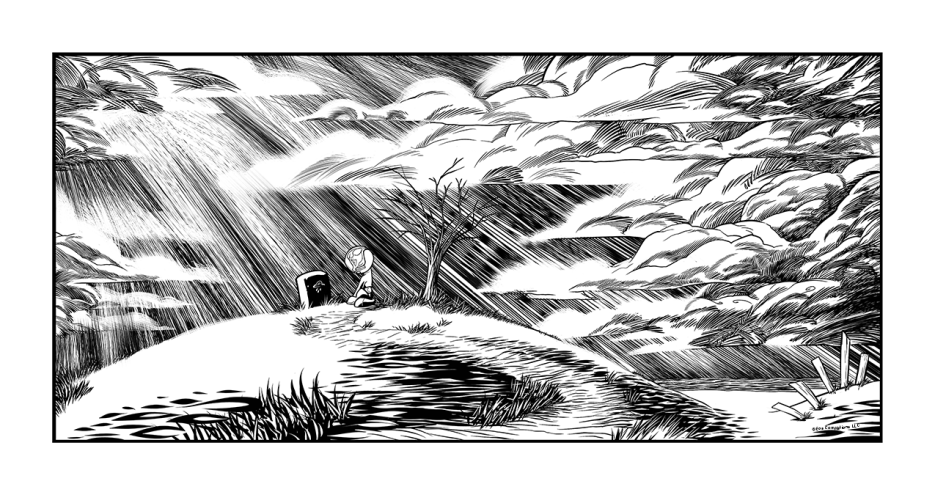
\includegraphics[width=\linewidth]{image19.png}

\begin{intro}
    当风吹起时,摇篮就会摇摆,
    
    When the bough breaks, the cradle with fall,

    \medskip

    当树枝断裂,摇篮和宝宝会一起掉下来。\footnote{这一句是经典摇篮曲 \emph{Rock A Bye Baby} 睡吧宝贝的歌词}

    and down will come baby, cradle and all.
\end{intro}

\daytimeplace{14}{10:30 AM}{翡翠海岸,52号国道南段}{Emerald Shores, Big 52 S Branch}

帕比骑着滑板车在她的小跟班身边飞来飞去绕着圈子。

「耶……!你碰不到我!我超级快!」

尸鬼蹦蹦跳跳地想要跟上帕比,从远处看就好像两个穿着防辐射服的小孩子在嬉戏一样。不过或许这也是她们正在做的事情。一路玩耍让她们去翡翠海岸的旅程稍微慢了一点,不过这样也没什么关系。

「喏,跟班,」帕比停了下来,看着她的伙伴,「我不太确定妈妈喜不喜欢丑丑马,不过我会跟她说你是我的好朋友,而且你也找不到妈妈了,她肯定会帮你修好你的箭头……呃……不过,别做奇怪的事情好么,比如说马尾伯爵做的那种……呃……好么?我可不想第一天见妈妈就被关家门……」

那个生物歪着头,帕比把这个表情当做是肯定的回答,「那好,我来过这里好几次了,这里超超级好玩,只要你不问漂漂马太多问题就不会被妈妈训斥……问问题不是错,只是有些马不太喜欢某些谈话内容。」比如说,问为什么小马可以光屁股在大街上跑,但是为什么去海滩就必须穿比基尼之类的……帕比完全不知道为什么!

\horizonline

\daytimeplace{14}{11:00 AM}{铁砧镇,52号国道南段}{Ironworks, Big 52 S Branch}

砰……!砰……!

强盗的脑袋像个西瓜一样爆开了,在坏枪的掩护下,扳机熟练地给她的霰弹枪换着弹药。

「我们最好赶紧,乐乐,铁骑卫肯定也在附近清理……」

附近的爆炸把泥土溅了他们一头。

装好子弹之后,快乐扳机拉了一下枪栓,「没错,如果我们不想被多开几个洞的话。」雌驹说着飞奔到一座帐篷边,「掩护我破门。」坏枪移动到另一边的时候,雌驹冲进里面举起枪。

砰!砰!轰隆!

「咿!」

一堆电子设备炸成了五颜六色的火花和碎片。\emph{打的好,乐乐,对于那些看起来像是机器的东西都是先打一枪再说。}这个帐篷里面有一张沙发,一堆箱子还有一台刚刚被她打爆的无线电……但是看起来里面一只小马也没有。

% TODO: 译文不合原文,此处改正

坏枪跟着走进来,「你愣什么呢?」

雌驹没有回答,警惕地看着周围,「我……我觉得刚刚好像听到一声惊呼……但是这里好像没有能发出惊呼的『漂漂马』。」

「那简单。」公马端起突击步枪,直接扫射了屋子一遍,在板条箱打了一排洞,打烂了小床,还把桌子上吃到一半的食物打成了一份现代派印象作品。然后他们听到了一声吃痛的惊叫,然后一个缩成一团的雌驹凭空出现在床底下,她肚子上的伤口留下一滩血。

「狗屎运……」乐乐喃喃自语,走进那个雌驹想一枪解除她的痛苦。她屁股后面有个白塔的可爱标记,那雌驹看起来那么年轻,一副失魂落魄的样子让卫兵迟疑起来。

「救救我……我还不想死……」独角兽闭着眼睛,在一阵阵剧痛带来的痉挛之间呻吟着,「妈妈……妈妈……救救我……」

「你等啥,她那样很痛苦的!」坏枪叹了口气走到那个雌驹身边举起枪。

「等等!」乐乐用蹄子推开公马的枪,她看着那个慢慢变得虚弱的雌驹,她还在祈求着她妈妈能来拯救她。

「我们……我们变成什么了?这个小马手无寸铁,只是躲在那里而已!」乐乐拿出一个治疗药水喂给她。

「你打算救活这家伙?为什么?她有机会绝对会毫不犹疑地杀了你!」坏枪不屑地打了一个响鼻,「而且她的『亲朋好友』说不定现在正在屠杀我们的盟友呢!」

乐乐回头白了那公马一眼,「你看到这个房间有任何武器么?」那个受伤的独角兽只剩下哭泣的力气了,不过乐乐还是给她喝了一些药水,「如果我们坚信,所有小马都是漂漂马,本性都是善良的,那么我们还是有机会重建昔日的小马国。」快乐扳机抱着小马要塞轻声唱着摇篮曲安慰着她。

坏枪坐在他的雌驹身边叹了口气,「你想太多了,总有一天会后悔。」

快乐扳机耸了耸肩继续唱。

\horizonline

\daytimeplace{14}{11:00 AM}{翡翠海岸,52号国道南段}{Emerald Shores, Big 52 S Branch}

帕比对面前的景象皱起了眉头,这里完全不是她记忆中的翡翠海岸!这里简直是一团糟,而且看不到一个马影!海边的所有小房子都变得脏兮兮的,而且海滩上也一片狼藉。

「怎么还没过多久这里就变成这样了?小马呢,音乐呢?婚礼庆祝呢?那些小店呢?还有……妈妈呢?」黄色的小雌驹伤心地低下了头,「抱歉,小跟班,看起来这里好像刚刚刮过台风。我想带你去玩旋转木马但是……」帕比回头用愧疚的眼神看着那个半腐烂的怪物,「我觉得现在那地方可能也没开门……」

那个尸鬼看起来毫不在意,但是帕比想给她的新朋友留下好的印象。

「哦,或许我们可以去看看糖果店好么?我们可以给妈妈准备个惊喜!」听起来是个不错的主意!给妈妈带上礼物一定能得到额外的抱抱和亲亲,「走,我们去商店血拼咯!」

小雌驹走下山丘,来到沿海的小镇上,小镇的建筑物都破旧不堪,窗户不是被打破了就是被木板钉上了,几乎城里的所有门都被木板封着。

「哇哦,刚刚过境的绝对是场大风暴!不过别担心,我知道有个买糖果的好地方!就在这个小巷子里面!」帕比一边说着,一边踩着小巷之中的水坑来到小路尽头。

「{\mt 警告,侦测到中等辐射,威胁等级:可忽略。}」

完全不管这个声音,小雌驹继续往前走着。

「{\mt 警告,侦测到大量辐射,威胁等级:可忽略。}」

帕比皱起眉头不爽地说:「喂喂,别胡说了,声音先生,拿出金币来!金闪闪的那种!我想要买好多好多糖果!」一堆金币浮到了小雌驹面前,她哼着歌转过拐角……{}

……{}

「这不公平!」

就在那个糖果店应该在的位置,现在是一个圆形的弹坑。帕比叹了口气,「好吧,好吧,别担心,我还知道很多可以买东西的地方。」不管怎么说,这里有很多很多小商店可以买好东西,怎么可能所有的商店都不见呢?

\horizonline

\daytimeplace{14}{11:15 AM}{铁砧镇,52号国道南段}{Ironworks, Big 52 S Branch}

白先生飘着一把来复枪从帐篷口探进头来。

「有谁受伤了?」

坏枪转头看着白苹果的老大说:「理论上是这样,刚刚我们打伤一个强盗,乐乐正给她急救呢。」

「哦,好吧,你们慢慢来,铁骑卫正在……等等,你说啥?」老白走进了帐篷看着那俩小马,「我们难道不就是来消灭他们的么?什么时候改变计划了?」

坏枪耸了耸肩,「你问他,好像和『漂漂马』啥的有关系。」

「闭嘴老枪,这个雌驹是非战斗成员!她只是带着隐形小马躲在床下而已,完全没有任何武器。我是个士兵,不是杀手。」快乐扳机一边说着一边用一个床单给雌驹盖好。

白先生摇了摇头,「我说,我们没时间搞这个了,野牛帮在撤退,我们必须立刻追击!我们没时间玩好马游戏了!我们越快结束这场战斗,就能越快在那个关于帕比的『阴影』什么预言落在我们头上之前赶过去。」

当听到帕比这个名字的时候,那个受伤的小马神经质地低语起来,「幽灵……是她在这个不洁之雾里召唤了不死同伴……她们是来吞噬你们的灵魂,是来杀死所有小马的!这都是我的错,我的错!为什么我要惹幽灵生气!妈妈……救命!」

「幽灵?不死?这只是个迷雾魔法而已,她在叨叨些什么?」白先生扬起了一边眉头。

坏枪清了清喉咙,「实际上,在来这里的路上,我们发现三个小马被……嗯……撕成了碎片。好像有谁用蹄子把他们给生撕了,那情景还真是挺可怕的。」

乐乐点点头,「没错,我们显然不是突袭这里的第一梯队……在我们之前,这里的小马已经在疯狂乱射了。」

白色的公马哼了一声,「真不错,这可以解释为什么还没等我们来这里就听见一堆枪声……不过现在有谁可以跟我解释她在念叨什么吗?」他戳了戳那个雌驹,「嘿,你能听到我说话么?你惹谁生气了?又是谁袭击你们了?」

「幽灵……52号国道的小幽灵……我们……不……是我……我打了她的屁股……她的泪水引来了恶魔……黄色幽灵……像她一样。但是……更残忍无情的不死怪物……她们杀了血浴……现在她们找我来了!是我打了她的屁股!是我打了屁股!全都是我的错!」

小马要塞歇斯底里地尖叫个不停,帐篷里面的三个小马一起用力才按住她。

「喂喂!冷静!这里没什么黄色恶魔!她们早走了,别挣扎,你还很虚弱!」坏枪终于坐在那个雌驹背上让她冷静下来。

「你……打了……帕比的……屁股?」白先生听到这里差点没忍住笑出来,「真的?我可是错过了最有趣的部分……」

\horizonline

\daytimeplace{14}{11:15 AM}{纪念碑镇,52号国道南段}{The Memorial, Big 52 S Branch}

「亲,你做得够好了。」

萍琪派坐在了长耳的身边。

先知长叹一声,从恍惚之中回过神来。

「我……好累……」

「亲,别担心,第一次都是这样的,不过你习惯这种感觉之后就好了。」

独角兽雌驹想要站起来,但是她的四条腿已经支撑不住自己的重量了。

「唉,到此为止了么?」

「还没……不过我觉得也没剩下多少了。亲你太过努力了,我早就警告过你,记得吗?」萍琪微笑起来,「不过别担心,一点痛苦都没有的,我们还可以一边等一边玩游戏!」

长耳露出一个虚弱的笑容,虽然死前还有个幻觉朋友可以聊天,不过在他乡异地因为毒品而孤独地死去,这个代价实在太高了——但是这一切都是有意义的。

「告诉我,她会一切平安么?」

「为什么问我?亲才是萨满哦!咱不过是个普通的漂漂马而已啦,哦,哦,你想要玩钉马尾游戏么?」

「求你了……我……我必须知道。」

叹了口气,萍琪皱起了眉头,「好吧,为啥大家全都这么无趣?好啦好啦,我说就是!她不会平安……至少现在不会,还需要最后一步,不过那个魔法迷雾相当不赖。」

独角兽虚弱地叹息,「那么,至少我死得还有价值……」

「亲,别皱眉都皱成梅干菜了!我们还要去准备派对呢!那个雾超级漂漂,把所有东西都掩盖了,帮了那些可怜的小幽灵一个大忙……至少你在最后一段旅程里给了那个小小幽灵一个可以陪伴她的朋友……不管怎么说,亲你逆转了命运!这绝对是值得庆祝的大喜事!呃……虽然把亲的小命搭上了,不过不管怎么说都应该高兴,不是么?」

……{}

「对吧?」

……{}

「哎,你看看她,又睡着了!好了!别睡了,起床了亲!我们该出发了,不然会迟到哦!」

\horizonline

\daytimeplace{14}{11:45 AM}{铁砧镇,52号国道南段}{Ironworks, Big 52 S Branch}

「你他妈跟老娘说什么?」赫瑞咆哮着,尖锐的喙几乎扎到了诘责的鼻尖,「什么叫『她不在这里』?」狮鹫完全不管其他铁骑卫对着她的枪口,继续对老书记官怒吼着。「你这个骗子!我信任你,干了你让我干的事情!现在你说她不见了?」

展开翅膀的狮鹫发出一声怒啸,对那掠食动物的吼叫毫不动容的诘责清了清喉咙,伸起蹄子示意那些铁骑卫放下枪。

「我知道我们曾经有过约定,不过她醒来以后自己跑掉了,你也知道那个孩子自个儿乱窜的时候想要让她呆在原地有多难,对吧?」

赫瑞塔眼底的岩浆似乎随时会喷发出来,「你知道现在她跑哪儿去了?」

诘责耸耸肩,「上一次见她的时候,她正往翡翠海岸去,不过我又不是先知……」

那佣兵面无表情地说:「我猜,她往南走了是吧。」

铁骑卫点点头,「就在海边,错不了。」

孤狼从旁观的马群里面走了出来,「等等,狮鹫,你想去那边的话,我和你一起去!」雄马展开翅膀跟上了赫瑞塔,「我觉得我们应该等等其他马,那里可能会有危险!」

「没错,等等,老娘等够了。在你们整个肏蛋奇蹄类动物里面,老娘只关心一位,而那位现在不在场……滚边儿去吧,小马!」赫瑞塔啐了一口,就好像要吐掉喙之中的恶心味道一样,然后张开翅膀消失在工厂屋顶之后。

「我现在就去追上她,你们尽快跟上我们好么。」

白先生以蹄覆面,「真是个好计划,先是单独行动,然后又是添油战术么,难道不是有什么南边的邪恶黑影啥的预言么?我们已经把我们那花里胡哨的专家丢在脑后了,现在又要分开行动。要我说,我们还是检查一下这里的生还者,然后决定怎么处理俘虏,最后等长耳来了一起往南走好么?」

「说到往南走……有谁看到融金了?」快乐扳机看着周围问。

天马嗤之以鼻,不耐烦地刨着地面,「这里有天杀的十五个铁骑卫!十五个!这群家伙绝对可以解决土匪的残兵败将,然后帮下面那些小马打开避难厩!现在我更关心那个幽灵而不是52号国道的地盘划分!我去追那狮鹫去了,你们最好也快点!这可不是个会等你们的派对,如果先知没错的话,我们时间不多了。」留下这几句话,孤狼飞走了。

\horizonline

\daytimeplace{14}{12:00 AM}{翡翠海岸,52号国道南段}{Emerald Shores, Big 52 S Branch}

帕比一点都不开心,她完全没找到任何给妈妈的礼物。或者说,她在整个城里连一只小马都没找到,这让她开始紧张起来。小雌驹觉得哪里不对劲,她开始担心妈妈会不会又跑到另一个地方去了。

所以她急忙冲向那个粉色箭头指向的海边小山丘,帕比在城里闲逛的时候,那个箭头一直没变过,不过帕比以前也遇到过这种事情,每一次旧的箭头消失就会有新的箭头出现,一次又一次地出现。

「好吧,小跟班,我们去找妈妈,或许这一次是对的!」

两个小孩子慢慢爬上泥泞的小小山路,这个山丘有一片微枯的黄绿色草坪,还有一颗死去很久的老树,帕比来到山顶的时候,她看到那里也有很多很多的小石头,每一块上都刻着一个名字和可爱标记,就像另一个爸爸的地方一样……好奇怪啊,为什么会有另一个爸爸的地方?

一只小马正坐在那颗只剩下枝干的树下,他慢慢站了起来,走向帕比和她的新朋友。

小雌驹飞奔向来者。

「妈咪!」

帕比的声音里充满了希望,但是很快又变小了。

「你……不是妈妈……」

在帕比身后的小跟班冲着来者发出了威胁的低吼声。

「不,帕比,我不是你的妈妈,抱歉……」融金用他那沙哑的声音说着,然后走到了一个布满苔藓的灰色石头面前,

「我真的……很抱歉……」

小雌驹走到了那个尸鬼身边,然后注意到那个粉色的箭头原来是指向这块石头的。虽然石头上的字迹早已经风化得模糊不清,不过她可以清楚地看到,那个一朵云和三点雨滴的可爱标记。

那是……妈妈的……可爱标记。

妈妈……{}

\horizonline

\daytimeplace{14}{12:00 AM}{翡翠海岸,52号国道南段}{Emerald Shores, Big 52 S Branch}

「好了,都安排好了。」白先生和诘责一起走了出来。

快乐扳机点点头。「好吧,那里一点都不远,我们别磨蹭了。」

诘责看着远处那个指示翡翠海岸方向的标志牌,只有六公里而已,天气好的时候都可以清楚看到小镇。

「如果那里情况不妙的话,我们要尽可能地拖延时间。」

「那还不赶紧!」快乐扳机说着沿着52大路开始向南边飞奔。

「好吧,谁最后到谁就是赤兔!」灌木笑着看了他叔叔和老书记官一眼,然后跟上那雌驹的速度。

诘责叹了口气,「这帮小年轻,他们绝对会在半路就累趴下的。」两个老公马跟着其他小马一起奔向海岸。

\horizonline

\daytimeplace{14}{12:10 AM}{翡翠海岸,52号国道南段}{Emerald Shores, Big 52 S Branch}

尸鬼什么也没说,只是静静地站在那里,让帕比有时间理解这个现实。

「妈妈……在这里?但是……」

小雌驹盯着这块石头,想要理解到底发生了什么,而跟班则坐在了头领身后。

「她……和爸爸……走了?但是……但是……不……不要……」帕比的声音越来越小,好像她声音太大的话,这个残酷的现实就无法改变一样。

「但是……我……我也想去……我……我想去见爸爸……为什么……为什么她把我留在家里?我……我……」

帕比失声痛哭起来。

「我真的没有不听话……我只是……我只是想要看烟火!我……我不知道我的房子会倒掉我妈妈会走掉……我……我……」帕比一屁股坐在了地上,低头看着自己的蹄子。

「只是想看那个破烟花而已……为什么接下来一切都一团糟!我很抱歉……我错了……我真的错了……对不起……妈妈……请回来呀!」

帕比嚎啕大哭,绝望地对着那块埋葬着她母亲的墓碑大声哭道:「妈妈!你……你说什么我都听!训我吧!打我吧!但是别扔下我啊!」

融金看着他面前的可怜生灵,想要说些什么,说任何事情,但是这一幕实在太过悲哀,让他说不出一个字。而这个时候,她抬起了头,于是那双泪流不止的双眸和他对上了。

「求求您,求求您告诉我妈妈去哪儿了!我把我的玩具给您好吗,我愿意把我所有东西都给您,好吗?还是您想要更多漂漂玻璃珠?我会为您把所有的玻璃珠都找到,好吗!求求您!求求您了!」帕比站起来走向那个老尸鬼,而小雌驹沉重的视线让他不由得后退了几步。

「帕比……我很抱歉,但是……这里就是你妈妈长眠的地方……她……已经死了……她很久很久之前就已经去世了。」

帕比笑了,但是那微笑毛骨悚然。那双空洞的眸子盯着融金,不住地颤抖着,「死了?只是死了?她死了?那没关系的!她会好起来的吧!我也已经死了,但是你看我很好啊!你也死了但是你也很好啊!死了没什么不好的对吧?我们只要在这里等就好了,对吧?对吧?对吧!」

融金看着那天真的小孩子,死了……还会好起来?只要在这里等?

「帕比……不是这样的……她……她已经不会回来了……她已经去世了……她已经……帕比……你可以跟我在一起,好么?我永远不会丢下你。虽然我不是你妈妈……」

「怎么有俩帕比?到底发生什么了?」赫瑞塔一个猛地降落在地上,压坏了好几根树枝。「僵尸,把你的脏蹄子从我朋友身上拿开!」狮鹫落在融金和帕比之间举起枪指着尸鬼。

黄色的小雌驹很快就认出了新来的狮鹫,「赫瑞!赫瑞!妈妈……妈妈……妈妈她……妈妈她不要我了……她和爸爸走了……丢下我不会回来了……我……我我……帮帮我!」

佣兵看了看那个用蹄子指着墓碑的尸鬼,然后明白了帕比在说什么。

「草泥马,老娘……来迟了……」

赫瑞塔转身用一只爪子抚摸着帕比的头盔,「帕比,我会陪你,好吗?你不会孤独的。」

「但是……我想我妈妈!我要我妈妈!她……只有她才能……只有她才能把一切都修好!她可以修好坏掉的房子,修好这个破太空服,找到跟班的妈妈,让之前快乐的日子再回来!没……没有她我都不知道该怎么办!」

什么也没说,狮鹫紧紧地抱住了帕比。

「但是……但是你自己就已经做的很好了,帕比……你救了我,你还救了整个太阳城!你还阻止了铁骑卫的内战!你还……你……你是个好孩子!你是我认识的唯一一只好小马!不需要你妈妈,你就可以解决一切。让我当你的姐姐,好么?赫瑞和帕比,最佳组合!」

「狮鹫说的没错,帕比……你已经长大了,你妈妈会为你自豪的。」

帕比挣扎着推开了赫瑞塔,她的双眸之中燃烧着粉色的火焰,「但是她把我丢在这里!她扔下我和爸爸一起走了!我那么爱她,为什么她要扔掉我?为什么她不爱我?」

「你丫到底想……」赫瑞塔摇了摇头,「你到底说什么呢?她没有选择扔下你,她只是迫不得已。她绝对不会丢下你不管,她以为你在避难厩里面会平平安安的长大,否则她绝对不会把你丢在这么危险的地方的!」

孤狼落了下来,「呃……我不知道发生了什么,但是我觉得对小孩子大喊大叫没什么用。」

「我说也是,狮鹫小姐,所以我一直不……」

帕比打断了那两个公马的碎碎念,大声吼着:「那么为什么她不回来接我一起去?」

「傻瓜,她已经死了!死了!懂不懂!」赫瑞塔锋利的喙顶着帕比的头盔,和小雌驹对视着,融金想拉开狮鹫,但是小跟班低吼着拦住了他。「妈妈不会再回来了!你已经永远失去她了!这就是命运!她现在就躺在这个坟墓里面,绝对!再也!!不会!!!回来了!!!!所以你要坚强起来,将你自己的命运踩在蹄下!别管那破墓碑了,现在就跟我走!」

狮鹫转头看着那个老木乃伊和天马,不过她马上注意到一大堆小马正在从北边赶来。

「看到没有?你的朋友来接你了!你让大家都担心坏了,别再这样失落了,伸出蹄子站起来好么!」

帕比看了看过来的马群,然后又看了看那个有可爱标记的墓碑。

「妈妈……在这里面?」

赫瑞塔完全没有注意到帕比的表情和融金拼命的示意,只是说着自己的话,

「没错,你妈永远都躺在这里,你什么时候想来看她都可以,现在跟我来,一起和你的朋友说你一切安好,好么?」

「石头!」

帕比尖叫着举起了「命运之石」,然后用力砸向那个墓碑。

「你丫在干什么?」赫瑞塔想阻止她的朋友,但是小跟班跳到了她们俩之间,即使是勇敢的狮鹫也被那双红色的眼睛吓住了。

「妈妈,妈妈出来啊!」帕比用她所有的力气砸着墓碑,融金和孤狼被这碎石飞溅的景象吓坏了。

「等等孩子!那样她也不会回来的!别这样,你会……你会打坏你妈妈的坟墓的!」孤狼跳了起来落在石头边挡住了帕比的蹄子。

「你到底怎么了?别这样!」

「放开……放开我……放开我!我想要妈妈!为什么妈妈不见了!」

跟班转头吼着天马的时候,赫瑞塔立刻冲过来打上帕比的头。

「傻瓜!给老娘振作起来啊!丫的真想打你的屁股!忘了你妈妈吧,傻瓜!你现在和我在一起了,别想不可能的事情,醒醒吧!」

被狮鹫的愤怒搞迷糊的帕比愣住了,小雌驹慢慢地转向大海,「但是……但是……我把她忘掉的话……我找不到妈妈的话……我……还能做什么呢?」

赫瑞挥着爪子说:「那我们就一起去找些快乐的事情来做,好么?你冷静下来,我会替你想办法的!乖乖的……乖乖的坐好……你看,你的朋友都在这里。」

老白,诘责,快乐扳机和坏枪正跑向山丘,虽然他们看起来精疲力竭,但是诘责还是喘着粗气问。

「发……发生什么了?」

帕比看了一眼蹄子中的「命运之石」,低声说:「我……我不想醒来……我只想……永远睡下去……再也不醒来……」

赫瑞塔拍着帕比的头盔微笑着:「我知道那种感觉……但是,总有一天会消失的,你也一样……乖乖坐在这里冷静一下,我们去招呼新来的小马,好么?」

黄色的小雌驹虚弱地点了点头,「命运之石」第一次从她蹄中滑落,滚下山丘,在山坡上来回弹了几下,最后随着一声金属敲击声落在了海滩上。

\horizonline

\daytimeplace{14}{12:25 AM}{翡翠海岸,52号国道南段}{Emerald Shores, Big 52 S Branch}

融金和孤狼已经走向了新来的马群,赫瑞塔也走了过去,把帕比和她的黄色小伙伴孤零零地留在坟墓边。

「别担心,她会好起来的,她现在只是需要独处一会儿。」

「但是……她在哭么?她怎么样了?」

帕比觉得如此……空虚。不是悲伤,也不是愤怒,也不是她以前感觉到的任何感情。她就在她妈妈面前,但是妈妈却不在这里,再也不会抱着她,对她微笑了……{}

「……虽然我不是那么多心,但是我还是想看看她的情况……」

「……那小心另一个尸鬼,那东西看起来蛮凶的……」

大家都在乱糟糟地说着什么,在帕比听来就是一阵嗡嗡的声音。帕比不关心,她只是慢慢地沉浸下去,慢慢地沉入内心深处。

再也见不到妈妈了。这个想法已经让她失去了所有力气,她顺着这条路走了这么远,唯一的目的就是想要再见到她的妈妈,但是现在什么也没有了。她很喜欢她的朋友,但是她觉得这样不对,这里根本不是她应该在的地方,她根本就不想呆在这种地方!或许……或许会有什么地方……不一样的地方……更好的地方……{}

「……那么就是这样了?我们做到了?52号国道安全了?那孩子也没事了?好了,我们现在回家吧……」

回家……家又在哪里?家已经没有了,她在中心城的家已经没有了,妈妈已经没有了,再也回不来了,再也见不到她了。帕比不想这样活着,她不想要这样……每一天晚上都醒着,直到凌明的曙光再一次提醒她又是没有妈妈陪伴的一天……她不想醒来,只想就这样睡去。

\py{「哦,那很简单,小家伙,你只要和我许个愿,我就会让你静静地睡去,做一个永远永远不会醒来的美梦。」}

「……闭嘴老枪!我们离开几天而已,隧道镇又不会烧了!」

「真的?你能做到么?」

\py{「那当然!我可是梦之主,我可以给你所有的快乐,你只要向我许个愿。」}

「……野牛帮还没完,我们只是把他们赶走而已,但是我觉得我们应该想出一个和平解决方案……」

「……我不觉得他们会同意的,老爸,野牛帮可不吃爱与宽容那一套……」

「……或许现在他们的王牌都打光了,他们会更……讲理……诘责,我觉得我们至少应该试试看……」

「永远永远的永远?」

\py{「比永远还要更长久,这是你我之间的约定哦。我可以让你在梦中和你爸爸妈妈永远过着幸福快乐的生活,而你嘛,只要让我在你睡着之后做一点点小事就好啦,可不可以啊?」}

小跟班尖叫着拼命戳着融金的后背,但是大家似乎全都更加专注于老白和诘责之间关于52号国道将来格局的讨论,没有注意那个小小的中心城尸鬼。

「我在52号国道混了这么多年了,我记得野牛帮最早可不是那么凶恶,他们只是52号国道上的游牧民,只是因为52号国道的每个居民点都对他们课以重税,但野牛帮在重税之下买不起任何他们想要的补给,所以他们才铤而走险……如果每一个族群都友善那么一点,也不会落得如此结果。」

「……我可不那么想……我祖父总是说野牛帮一直在找机会咬你一口……」

「……第一个对野牛帮课税的就是老白你祖父!你难道一点想要改变这个的常识都没有么?」

一声悠长的叹息,帕比点点头,「好的,就那么做吧!」

\py{「你的选择很正确,你绝对不会后悔的。」}

「做什么啊,帕比,我虽然很喜欢你,但是废除马头税可没那么简单,大人说话小孩子别插嘴好么!」

「对,没错,请……让这一切都消失吧。」

\py{「我真是太喜欢你的天真纯洁了……我会想念你的,来吧,请闭上你的眼睛……」}

~\vfill

\begin{note}
    升级 (Lv 18) 

    新技能解锁:就是现在!——你立即升一级。

\end{note}

\begin{note}
    升级 (Lv 19) 

    新技能解锁:专注射击——在S.A.T.S.状态下,你瞄准对手的特别部位时得到5\%的命中率加成……你想说啥,帕比已经绝望到开始胡乱选专长了,她根本没有S.A.T.S.!

    新任务专长解锁:移动梦魇(等级3)——耶!你现在就是梦魇了!不过这对你的社交生活没什么好处,因为你对所有派系的声望都变成了敌视。至于属性奖励就不在这里写了,因为太长写不下了。
\end{note}



\chapter{路之尽头}

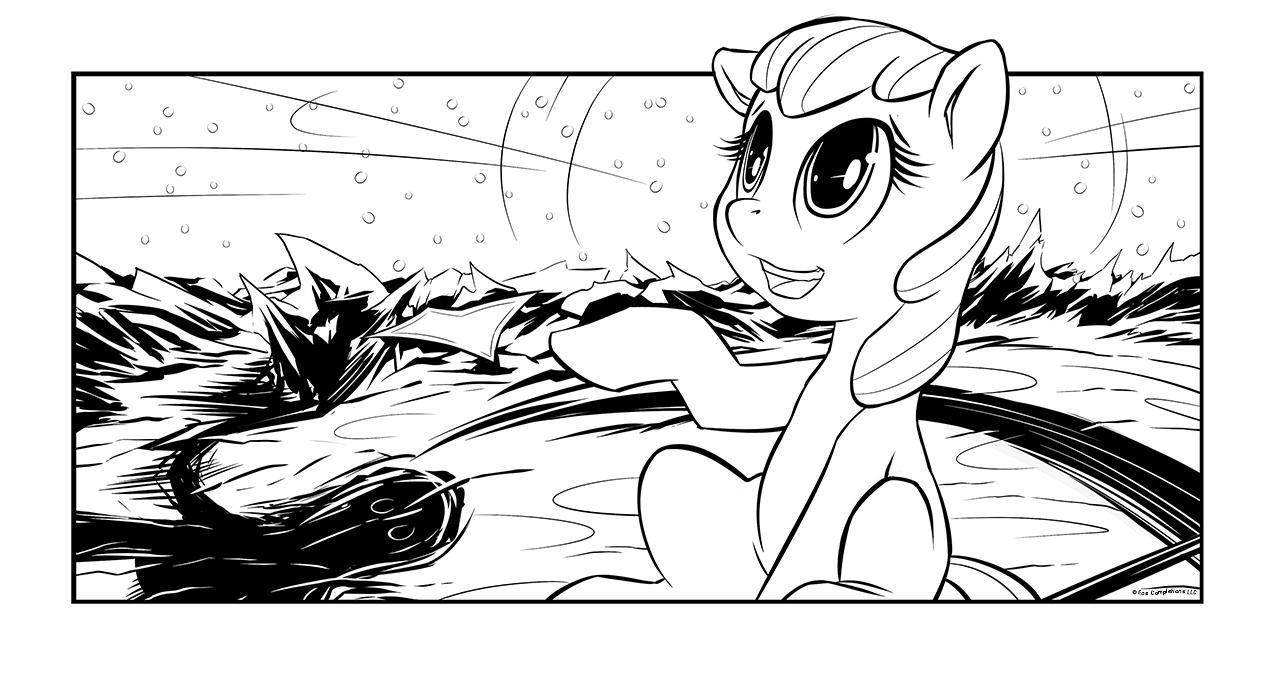
\includegraphics[width=0.9\linewidth]{image20.png}

\begin{intro}
    派对结束的时候,大家一起来个大拥抱吧!
\end{intro}

\daytimeplace{14}{12:35 AM}{翡翠海岸,52号国道南段}{Emerald Shores, Big 52 S Branch}

在拍打着海岸的阵阵波涛声中,帕比孤零零地面对着墓碑,而她的朋友在不远处争吵着。不过她唯一听到的就是在她脑中的低语,那个承诺给她美梦的低语。

「对,没错,请……让这一切都消失吧。」

赫瑞塔模模糊糊地听到帕比在她身后的低声念着,然后忽然感觉到一阵莫名的寒意,就好像刮起了一阵阴冷的夜风……她忽然觉得小雌驹刚才说的话有点不对劲。

大家全都回头看着快乐帕比,她在自言自语什么呢?消失?怎么消失?

赫瑞塔走过去,她可以看到帕比低着头闭着眼睛。小雌驹的鬃毛已经从之前的金色完全变成了夜空色。

「帕比?你还好吗?我……我觉得你鬃毛是不是有点……」

当帕比再一次开口说话的时候,却是另一个完全不同的声音,深沉而阴森,就好像在洞穴深处不断回荡的呼号。

「本宫终于亲临这个世界了,吾卑微的子民,还不赶紧对汝之新公主跪拜行礼!」

赫瑞塔歪着头挑起眉毛,「你丫说什么乱七八糟的,帕比?搞什么啊?」

小跟班的眼睛从红色变成了蓝色,慢慢走到帕比身后,像个卫兵一样笔挺地站着。那个黑化的帕比又说话了。

「本宫可不是快乐帕比,本宫乃星之子,怕音!汝等蝼蚁之辈的新公主,本宫将领导小马国崛起!」

诘责摇了摇头,看着融金问:「星啥?听起来像是某种上古斑马故事,星星什么的?」

老书记官的问题被赫瑞塔的暴笑打断了。

「怕音?你这个大反派的名字也太寒酸了吧,怕音是什么东东啊?你是自己想的么?」

羞得满脸通红的黑化帕比后退了一步,不过很快就恼羞成怒地大喝起来。「名字……名字什么的……收声,不准笑,愚民!这是汝等新公主之大名,还不快给本宫跪下!然后回到尔等故乡去宣布本宫临幸这个世界!」

快乐扳机嗤之以鼻,往前跨了一步,「不然呢?」

在怕音眼中的夜空色光芒一下子扩展到了小雌驹的全身。在她头上形成一个尖角,同时在背后展开了一对虚无的翅膀。

「不然,本宫会吞噬汝等灵魂!」

乐乐呆呆地看着那雌驹,而孤狼低声问诘责:「她能吃掉灵魂么?」

书记官看了看DJ,耸耸肩,「我怎么知道,如果她真是某种斑马黑魔法的产物……大概可以?不过我觉得她现在还没那么强。」

天马冷笑一声,「那就是不行啦?」

「并不全是,她还在显现阶段。你看她的翅膀和角还都只是虚影,而我想我知道怎么结束这场闹剧。」

在乐乐和那个生物对峙的时候,书记官低声和其他小马商讨着对策。

「我想我可以切断那个星灵和帕比的灵魂链接……如果怕音……呃……那东西没有灵魂以供给养,她就没办法在这个世界显现,自然就会被放逐回星界。」

「那么,你还等啥,邀请函么?」尸鬼问。

「不,我没办法自己施展这个魔法,这是一个又强大又复杂的法术,是一种超聚魔法,需要多个独角兽来施展……」

老赏金猎手说:「那么,你是想说,我们要被这个有这么孩子气名字的逗逼日翻了么?」

「喂,怎么,你们这些书呆子有什么好办法没有?」老白的脑袋挤进这仨小马围成的圈子中。

「技术上说,有,不过我需要几分钟搞定细节问题,帮快乐扳机让怕……这名字实在是……唉。」老书记官以蹄覆面,「好吧,反正让她忙着聊天,给我们争取点时间。」

老白点点头,然后走向另外仨马——赫瑞塔,坏枪和快乐扳机。

「我说,公主殿下,您刚才好像说了什么小马国崛起啥的?您可以详细说明一下如何做到么?别在没用的地方磨嘴皮了。」

梦魇暂时放下和赫瑞关于白痴名字问题的无营养争吵,转向新来的小马。「那易如反蹄,本宫的魔法比此等鼠辈强大万倍,本宫可以用法术治愈这腐朽的大陆,然后翻开小马国的新篇章!本宫决不允许吾之子民相互伤害,汝等粗鄙之辈的血腥争斗将被画上句号,汝等应该为本宫建造宏伟宫殿。汝只要为本宫送上贡品,而本宫将会解决汝等的一切问题!」

老白点了点头然后说:「好吧,听起来像那么回事……不过……你刚才说过贡品什么的是什么意思?」

那圣灵得意地坐下来,眼睛都乐得眯起来了,享受着被顶礼膜拜的快乐,「那是当然,本宫作为汝等的主宰。自然会要汝等做出一些……牺牲。嗯……每次满月的时候,每个城市献上一位小马做祭品就可以了,然后本宫会净化这片大地,保证汝等在本宫的统治下衣食无忧!」

乐乐皱起了眉头。「你……你要活祭做什么?」

怕音挥了挥蹄子,「和汝等无关。」

赫瑞和乐乐都惊得张大了嘴。雌驹正准备举起枪的时候,她注意到了老白的暗示又放下了。

这时候赫瑞说话了:「那么……你会把帕比还给我们么?」

梦魇有些惊讶的眨了眨眼睛,「什么,她才不会回来,在谁也不能伤害到她的地方,她正安享美梦,此乃吾等之约定!」

听到这句话,乐乐顿时大怒:「你说啥?帕比那么天真的孩子你都要骗,你的那些美梦全都是不存在的幻影!你……你居然欺骗一个孩子,骗她把美梦当成现实!放她回来!」

那怪物大笑起来:「汝等可笑至极!为何本宫会放弃如此甜美的灵魂美味,在她母亲陪伴的美梦之中,她将会长眠,从此彻底消失,这个残酷世界再也不会伤她分毫了。本宫绝不会再让那个孩子被你们所谓的现实所伤害。所以,那孩子将长眠不醒。另外,本宫特别开恩,提拔诸位成为本宫的信使,汝等现在就去小马国告诉子民本宫的驾临吧!」

「简而言之,」赫瑞抬着头,「你就是梦魇之月?」

「嗯,本宫尚未……好吧……正是……本宫是说……梦魇之月乃是比本宫更加古老而强大的前辈……」那个圣灵似乎陷入了沉思,不过马上又抬起头来,「不过本宫也足够让汝闭上那臭喙!」

赫瑞塔冷笑不已,「那么,简单的说,你丫还是个菜逼。嗯,梦魇菜逼。」

快乐扳机被这一句话逗得再也忍不住了,捂着肚子在地上笑得打滚,老白以蹄覆面,而其他三个小马回头看着这边,很好奇发生了什么。

「不准笑!本宫生气了!这个世界有这么多子民,本宫才不需要汝等……一……二……呃……反正很多个无用的笨蛋!」

赫瑞塔嗤之以鼻,「……你丫连四都数不到,就别装逼了好么?」

「汝……汝这个……蠢材!汝将付出代价!」

「不,她才不会!怪物!看招!」诘责站在了赫瑞塔面前,直视着梦魇的双眸,「以科学之名,我们会将你永远放逐!」

「哟呵?」那怪物咯咯笑着,虽然还气得满脸通红,但仍然不屑地挥了挥蹄子,「别逗本宫发笑了,科学?汝等是否明白本宫乃是何等存在?看在梦魇之月的份上,别说梦话了好么?」

诘责微微一笑,「你想听细节?好吧,仔细听好,我之前早就检查过帕比的防护服了,你能在这里显现的原因不过是因为某个呆瓜把死灵法术当生命维持法术用而已。不过我已经知道怎么纠正这个可怕的谬误了。虽然那魔法晶片几乎坚不可摧,但那里面的魔法却没那么稳定,这就是为啥你的翅膀和角还都只是虚无的火焰。不过现在这里有好几个独角兽,虽然他们不懂啥叫『魔法裂解术』,但我可以直接使用他们的魔力来施展这个超聚魔法。那么,现在猜猜看这个『魔法裂解术』要用在谁身上呢?」

「什……什么……?」那个梦魇大惊失色,后退几步。

「好了各位,我要准备法术了,你们只要放空脑子让我接管你们的力量,然后这场梦魇闹剧就此结束了!」

一道闪光从诘责的角尖上炸开,光芒跳跃到几个独角兽的角上,他们都一起将那个魔力聚集起来为超聚魔法添加魔力。

乐乐闭上眼睛,让魔力透过她的身体,然后坏枪和老白也一起做了,很快他们的角也一起发出同样炙热的光芒,照亮了整个山丘。

赫瑞塔被这强光逼得微微后退闭上眼睛,不过诘责刚才说的话让她很担心,他打算摧毁那个防护服上用作生命维持的死灵法术来毁灭那个梦魇,但那不是让帕比活着的东西么?

赫瑞塔转头对老书记官大叫着:「等等!你想杀了帕比么?」

诘责没有回答,但是被白光照亮的那个怪物惊恐的尖叫让赫瑞确认了自己的担忧。

「愚蠢之辈,如果你解除那个魔法,那孩子会和我一起死的!」

「不行,肏蛋!给老娘停下!你不能杀了帕比,天杀的独角兽!」赫瑞塔怒吼着冲向诘责,把他撞飞了出去,诘责仰面朝天地摔倒,失去了法术的专注。

那个白光射出的彩虹失去了焦点,飞得到处都是,就好像一个坏掉的迪斯科彩灯一样到处飞。

梦魇菜逼或者说怕音,小心地睁开眼睛,不知道发生了什么,不过看起来自己毫发无伤,看着面前几只满脸莫名其妙的小马,她的脸上露出了邪恶的微笑。

「哈……不管怎么说,帕比的狮鹫朋友最后还是有点用处的。下次挑战本宫之时,汝等还是别拉这种猪队友入伙了。」怪物大笑着:「噢,本宫说什么笑话呢,汝等已经没有下次了,因为汝等鼠辈现在就去死吧!」

诘责摇摇头站了起来,被赫瑞塔刚才那一撞搞的莫名其妙,「你……你为什么要打断魔法!你这个脑子里塞羽毛的蠢货!那法术就要完成了!」

另外几个独角兽也满脸恍惚,显然是被强力魔法的消耗搞得精疲力竭。融金正在推醒老白,赫瑞塔则冲向诘责,用爪子指着他叫着,「你……你不能把帕比从我身边带走!一定还有其它解决办法的,绝对会有的!」

「蠢货!那孩子已经死了!我们是在拯救52号国道!从你那快乐结局的美梦中醒来好么!」诘责怒斥着狮鹫,因为他们决胜的王牌被她给搞砸了,这样会害死很多小马。

梦魇享受着她对手的胜利美梦破灭的瞬间,「汝等的争吵何等有趣,本宫还真想再多欣赏一番,看鼠辈的丑恶内讧也是不错的消遣。不过现在本宫很忙,还有个王国要去统治。」怕音看了看双眸已经完全变成深空蓝色的跟班,那个中心城尸鬼已经变成了她忠心耿耿的侍卫,「游戏就此开始了。去吧,我的爪牙,教训这个臭嘴小鸡!」

跟班像猫扑老鼠一样扑向赫瑞塔,正在和诘责争吵的狮鹫完全没有注意到冲上来的尸鬼,甚至都没听到乐乐的警告。

尸鬼撞上狮鹫,扭作一团从山坡上滚了下去,赫瑞本能的反抗着,她的动物本能让她躲开了那小孩子强大的超自然力量,并且快速地反击着。他们化作一团蹄子和爪子的残影摔落到下面的海滩上。

看着她的爪牙和狮鹫滚出了视线,怕音叹了口气,「好吧,坏小鸡弄坏了我的玩具,看起来本宫还是自己动蹄……那么,谁想先死?」

孤狼和融金交换了一下视线,然后快速地跳起来把弹夹打空,子弹就像穿过黄油一样打穿了梦魇的身体。

帕比的胸口被打成了筛子,但是看起来完全没有用,因为下一瞬间那些洞都消失了。

「想要杀一个已经死掉的生物,是不是有点难度?」

怕音咯咯笑着用魔法抓起孤狼,然后把他扔向了一棵树。那天马重重撞在树桩上,随着一声黏黏糊糊的骨折声,倒在了地上,整个身体都向后弯折成了一个诡异的角度。

不过梦魇没有理会孤狼是不是死透了,转头面对着坏枪,「本宫看到汝还是拖家带口的来,何其可爱。汝等是想和那些老掉牙的戏剧一样『但求同年同月同日死么』?汝等有何遗言?」

「有,」老白举起包包里面的步话机,打断了怕音,「B计划,」他眯起了眼睛,「我们叫兄弟!」

远处传来一声炸雷,随之一发精确的狙击打穿了帕比的头盔,还轰掉了她的一条腿。

受伤的梦魇怒号着张开翅膀,飞上天空从云中招来闪电,雷霆如利剑般击中了远处的摩天轮,那个巨大的马造钢铁建筑在一阵烟尘之中轰然倒塌。

「不!灌木!」老白看着他侄子之前在的狙击位置已经成为一片废墟,这个……他完全没有想到会发生这种事情!

一排地对空导弹拖着长长的尾迹飞向天空中的梦魇,然后在她身边爆炸成无数火球,照亮了整个昏暗的天空。在他们的掩体之中,每一位铁骑卫都举起了他们的武器,向怪物的方向开始狂轰滥炸。

战斗开始了。

\horizonline

又黑,又冷,又湿,赫瑞塔呻吟着,她全身的骨头都在哀嚎,她完全不知道发生了什么,就记得有什么事情不对头。

在一阵粉色光芒中,有个甜甜的女声在低声耳语。

\emph{「亲,别担心,不过是你这个大坏蛋又干坏事了……没别的!」}

「坏啥?我死了?」狮鹫头疼得更厉害了,远处可以依稀听得到小马的尖叫声和爆炸声。但她可以清楚地感觉到,有什么东西,像是个粉色圆点,在她脑中跳跃着。

\emph{「笨笨小鸡,亲还没死呢。只不过是从六米高的高度大头朝下掉下来然后倒栽葱撞到烂石滩的后遗症而已啦。不过我可以肯定亲一点伤疤都不会有的!黛茜酱天天这么坠机也完全没有事!」}

「帕比?她怎么样了!我要救她!」

那个粉色圆点跳了跳,语气听起来就像是大姐姐在教训小孩子一样。\emph{「真的吗?但是看起来亲只是想要满足自己而已嘛!」}

「你……你他喵的叨叨什么鬼!我只想让她安全!」

\emph{「然后呢,让她永远永远都陪亲么?亲到底是想救谁,是可怜的小帕比,还是孤单的小赫瑞?」}

「老娘……我……我不知道……我只是想让她开心,让她露出笑容!她是如此特别,就像整个灰暗世界的一抹艳丽的色彩……我不想失去她,但是她除了自己妈妈什么都不想……就像……活在一个噩梦之中。」

\emph{「或许,她只是在做一个不知道如何醒来的美梦。或许,她需要她最最最要的朋友给她一点点点帮助。」}那个声音开始变化了,从一开始年轻雌驹的声音变成了一个老马的声音,但却又无比熟悉,让她想起来了太阳城那几天。\emph{「只剩下最后一步,找到帕比的「命运之石」,然后完成它的使命。」}

深吸一口气,赫瑞塔睁开了眼睛,发现自己正躺在乱石滩上。不远处是一个摔得粉身碎骨的太空士官长小跟班。那个生物似乎吸收了他们俩坠落的所有冲击力,现在就像一颗压扁的黄色橡皮糖一样贴在地上。赫瑞举起手枪,给那东西脑袋上补了两发,确保它完全死透彻了,然后检查周围。

在她头上,有一只小马被梦魇的夜空色魔法包围着,惨叫着飞出两百多米,然后啪叽一声栽进海里。

赫瑞没有理会那些上面那些战斗的喧嚣,给自己灌下一瓶治疗药水,开始找那块破石头。

「帕比的石头,帕比的石头!他妈的老娘怎么从这么多破石头中找一块石头?命运你妹的石头!」狮鹫恼怒地踢飞一块石头,那石头飞向一个生锈的铁盒子之后反弹的飞起来,在空中打着转,然后不偏不倚正中狮鹫双目之间。

「肏!」狮鹫一边揉着她的脑门一边捡起那块石头,她记得这块石头打中自己的声音,「这是你丫最后一次砸老娘的脑袋……然后……然后该干啥?你打中一个金属盒子,破石头,你想说啥?你是某种石头先知么?」赫瑞塔骂骂咧咧地走向那盒子,然后用「命运之石」砸向那盒子上的锁头。

「终于……」

咣!

「你丫……」

咣!

「还算……」

咣!

「有点用!」

咣当!

「很好,我们看看宝箱里面藏了什么?」

里面有几张纸片,一个老旧的阿杰玩偶,一些照片,赫瑞拿起照片看着他们。

其中之一是快乐帕比,不过稍微小一点,而且没有穿防护服,她正在插着四根蜡烛的大蛋糕面前开心地笑着,后面还有一些小马,看起来像是一个生日派对。

第二张照片是一个白色公马和紫色雌驹,他们站在一个老木牌面前,看起来他们是在苹果鲁萨门口,在两个小马之间坐着一个噘着嘴的快乐帕比,好像她不想拍照片或者完全不想去那里的样子。那个小雌驹看起来很年轻,或许只有三岁的样子……赫瑞塔转过照片,背面有一行字:「最后一次全家旅行。」

第三章照片是帕比穿着一件罩衫,带着一个蓝色的大大蝴蝶结,她正开心地笑着展示自己的新裙子,这一次在前面写着字,「帕比第一天去幼儿园」。

在最后一张照片的背面,年轻的佣兵发现后面写着这几行字。

\medskip

\wrpr{不管在哪里,不管是什么时候,在那遥远的彼端,我们会和爸爸再一次相聚。我以你为傲,妈咪永远会喜欢她的小小太阳。}

\wrpr{我爱你!}

\begin{flushright}
    \textbf{妈妈}
\end{flushright}

\medskip

一发导弹凌空爆炸,闪光照亮了赫瑞脸上流下的两行泪水。

佣兵叹了口气,终于抹去了模糊了双眼的泪,「她……她不属于这个地方……」赫瑞塔放下这些照片,「肏他娘,为什么要这样?为什么?!」

新的爆炸将天空染得火红,小马在那里和已经死去的东西战斗着,不断地死去,只是因为她自私地想要把幼驹留在自己身边。现在赫瑞知道自己该做什么了,虽然,这不意味着她真的想要这么做。

「不公平……这不公平……」

\horizonline

帕拉丁高斯瞪大眼睛,看着他发射的导弹在空中掉了个头,又朝自己飞了回来。

「高斯!」冷浴惊恐而无助地看着她最好的朋友在爆炸中消失,她愤怒而痛苦的视线转向梦魇,「臭婊子,为什么你不去死!」在她动力装甲两侧的转轮机炮疯狂地喷射着火舌,但是即使她打光了子弹,那个怪物也只是狂笑着把另一个新兵丢进大海。

怕音已经杀了两个铁骑卫,还把好几个小马丢进了大海,不过怎么才能一劳永逸地消灭这些家伙呢?这些笨蛋真的不知道什么叫决斗的规矩!她现在开始有点不耐烦了。虽然说杀掉小马很有趣,不过现在看起来这些家伙简直烦不胜烦,前仆后继根本杀不光的样子。而且她现在可有更重要的事情要做——比如说,统治世界之类的。

那么擒贼先擒王,这些蠢蛋的老大是谁呢?哦,对了,那个老书记官……怕音因为自己的小小邪恶脑瓜而坏笑着,「我说,穿披风的家伙在哪儿啊?」怕音落在老马的面前,张开她夜空色的翅膀邪笑着,「在这里啊,诘责,是吧?」就在那独角兽因为小雌驹心情突然变化而奇怪的时候,梦魇的笑容变得无比凶恶,「那么,去死吧!」怪物用魔法抓起老马的心脏,然后用力一捏,诘责闷哼一声倒了下去。

这个时候,赫瑞塔从悬崖边飞了上来,落在小山丘上的墓地边,面前的景象让她心中一紧。这都是她自私的错,小马在战斗,小马在死去,帕比绝对不会想要这样,该是结束这一切的时候了!

「帕比!帕比!听我说!」

不耐烦地叹了口气,梦魇转向狮鹫,「我说,还没轮到你呢?知道先来后到吗,等我先把这个杀掉之后再来杀掉你,别着急行不行?」

快乐扳机艰难地爬向诘责,卫兵雌驹绝望地想把老书记官救活过来。他们的抵抗就像纸片一样被小孩子扯得粉碎:融金正在那根穿透了他身体的树干上拼命挣扎着想要脱身,孤狼早因为脊椎骨折而昏了过去,即使是那些精锐的铁骑卫也被打得节节败退。难道这就是世界末日了么?他们都要死在这里了么?那一瞬间,乐乐觉得很伤心,她本来也想要个自己的孩子,这不公平……{}

「帕比,醒醒!你……你可以去见你妈妈的,真的!」赫瑞塔用她最高的声音尖叫着,她的嗓门确实很烦,「这臭不要脸的梦魇在骗你,你比她厉害多了!你是最棒的!」

黑化帕比哼了一声:「等不及去死了么?」夜空色魔法光芒笼罩在一块大石头上,然后径直朝狮鹫砸去,但是赫瑞灵巧地躲开了石块。「坏小鸡,别让本宫动怒好么。」

赫瑞塔直飞上天空,一个俯冲扑了上来,脑门紧紧地贴上了帕比的玻璃头盔,「帕比你这个笨蛋!你已经死了!死了!和你妈妈一样死翘翘了!难道你笨得连怎么死都不知道?别管这个蠢蛋,去找你的父母吧!」

「什么?」梦魇眨了眨眼睛,被狮鹫的突袭吓了一跳,她在说什么?她在和帕比说话?不……不不不不不……不可以!

「收声,她听不到你!」

「帕比,醒醒啊!你不用再留在这个世界了!我不需要你陪我!你应该离开了!我没关系……真的……」

一道夜空色的光芒笼罩了赫瑞塔的全身,让她身体在扭曲中发出断裂的脆响。怕音瞪着佣兵的双眸,她的声音充满了愤怒,充满了憎恶,「去!死!吧!」

赫瑞塔无法抵抗那强力的魔法,只是虚弱地笑着。

「帕比……你妈妈……就在那遥远的彼端……」

\horizonline

坐在一个池塘前,快乐帕比看着里面游泳的鱼儿,她周围的一切都如此宁静。皑皑白雪就像是星星从天上落下一般,覆盖了整个世界。她不觉得快乐,但是也不觉得悲伤,就像是在发呆一样,万事万物都模糊不清,也没什么意义。只有她,雪,还有水里的鱼儿。

帕比不记得自己在这里呆了多久,不过那不重要,她只是想忘记……忘记那些不想回忆的痛苦,或许真的有效,直到一条奇怪的金鱼从池塘里面探出头来。

「帕比你这个笨蛋!你已经死了!」

「虾米?」小雌驹歪着头,然后看了看自己的蹄子和尾巴,「我才没死,笨笨鱼!」

另一条鱼从池塘里面抬起头来,用女孩的声音说:「帕比,醒醒啊!你不用再留在这个世界了!」

「赫瑞?你怎么变成鱼了?」帕比咯咯笑着,「笨赫瑞,鱼不会说话的。」

寒霜开始冻结池塘的表面,但是第三条鱼从水中跳了出来,用赫瑞的声音说:「妈妈就在那遥远的彼端!」

\rcpr{「妈妈,爸爸去哪了?」}

\rcpr{「帕比,爸爸就在那彩虹的另一边……」}

\rcpr{「他……他会回来吗?」}

\rcpr{妈妈没有回答,但是帕比真的好想,好想,好想再见一次爸爸。}

\rcpr{「我……我们可以去找他么?」}

\rcpr{「没错,帕比……总有一天,不过不是明天,或者后天……在另外一个地方,在另外一个时间……我们最终会再一次团聚,好么?就是……就是在那遥远的彼端。」}

\rcpr{「萍琪毒誓?」}

\rcpr{「诚心发誓天上飞……」}

「眼里塞个蛋糕杯……」

帕比看着天空……终于看到了他。

「这次我是真的真的迟到了,虽然这个宇宙的所有时间都属于我,不过最近事情真的太多了,让我足足迟到两百多年!我可真不想来这里啊。」穿着黑色兜帽的骷髅马朝帕比走来。不过他看起来在自言自语,而不是在和帕比说话。

小雌驹笑了出来,那骷髅马真的好有趣,他就像那些坏脾气的退伍军马一样叨叨个不停。

「嗨,我是快乐帕比!你见过我妈妈么?」

「拜托!千万别祈祷!我要辞职了,或者退休了,或者先辞职再退休!」

骷髅马被小雌驹的咯咯笑声打断了。

「哇哦,骷髅马好有趣!」

停下了抱怨,那个灵魂收割者终于注意到了那个幼驹正在看着他,「你……你可以看到我?这是什么恶作剧么?如果这次又是恶作剧的话我真的要投降了……」

帕比歪着头。「恶作剧?绝对不是!上次我恶作剧我可是挨了好一顿打!」

那小马长舒一口气,然后坐了下来,「终于……」

帕比走到那个奇怪的公马身边,嗅着他的衣服,「呃……你是谁啊,漂漂骷髅马?」

「我?我是灵魂收割者,死神,终末,黑马……」看着那小雌驹一脸不解地眨着眼睛,骷髅发现自己只是在浪费好词,「不过那都是些无聊的名讳,我是那个引导小马走向他们来世的家伙。」

帕比一脸迷糊的表情问:「那么……你到底见过我妈妈没有?」

骷髅摇了摇头,「你还真是麻烦……」一张写着粉色字的银色机票轻轻飘落在帕比蹄子上,「小家伙,拿好这张银色机票,这可是给你的特快专机,感谢我吧!」

帕比睁大了眼睛,「我……我要去见妈妈了么?真的么?再也没有什么粉色箭头,或者坏机器,或者倒塌房子……只有……妈妈?」

死神点了点头,「没错,抱歉之前让你受苦了,让我以我自己的方式向你表达之前没有帮助你的歉意。」

帕比完全没有听到后半句,因为她已经开心的一蹦三尺高,「耶!」小雌驹紧紧抱了抱骷髅,然后回头看了一眼完全冻结的池塘。

「哦,对了,赫瑞!我要和我的朋友道别!」帕比转过头来,整个雪景顿时化作无数碎片,消失得无影无踪

她回到了那个墓地边的战场。

\horizonline

「……在那遥远的彼端……」狮鹫说完这句话之后,她双目失去焦点,昏了过去。

不过她刚刚说完这句话,那个梦魇的双眸就重新亮起了粉色的光芒,她的表情也完全变了,「拜拜赫瑞!一个漂漂骷髅马送我去妈妈在的地方了!还有一个超级闪闪的机票!」

最后一次,帕比眼中的粉色光芒消失了,她面前的HUD上亮起了红色的惊叹号。

「{\mt 警告,目标001快乐帕比无法定位,电池电量严重不足,警告,自动修理功能无响应,警告,硬件错误:未找到硬件。警告,即将关机,五……四……三……感谢您选择和平部,祝您有健康美好的一天,保重!}」

说完这些话之后,整个头盔上的HUD都消失了,只剩下怕音那张惊恐的脸瞪着空空如也的头盔。

那个怪物的魔力也消失了,被抓着的狮鹫落在不远处的山丘上,「汝等干了什么好事,蠢货!本宫要立刻杀了你们!汝等蝼蚁之辈!」展开它的翅膀,怪物想要放出一波新的魔法,但是她似乎有什么不对劲,因为那件防辐射服活像个破旧的皮球一样开始四处漏气,「怎么回事……本宫……我……我要融化了……不……不要!」粉色的气体从布料上的每一个破洞泄露出去,此刻,那个怪物身体只剩下一个完全的空壳。

「汝等!你们\ldots 你们别高兴得太早!本宫还会回来的!小马总会犯同样的错误,我要……啊啊!」梦魇的小脸化成了一滩粉色的粘液,把整个玻璃头盔溅成了粉色,一瞬间那个防辐射服似乎像个派对气球一样膨胀起来,然后在梦魇声调越来越高的尖叫中发出漏气的声音,像个被扎破的气球一样瘪了下去。

所有还能站起来的小马急忙抓起其他伤员,快速远离那团粉色的毒云。

「快走!赶紧躲开那东西!」冷浴抓起高斯的遗体紧跟着其他马。

在怕音的尖叫声中,小马四散而逃。

被半拖半拽的赫瑞塔期初还有点迷糊,所有东西觉得都非常遥远,她觉得自己好像在看不到的波涛之中上下起伏,在那恍惚的时候,佣兵好像听到了帕比的声音。

「喂……喂喂赫瑞!」

狮鹫呻吟着,那小鬼头从来不知道狮鹫的起床气有多大,如果她总是这样的话……{}

帕比显然不管赫瑞塔心中的抱怨,「听我说!我没什么时间了,但是我真的真的真的对不起,我真的要走了……我……我们还是朋友,对吧?」

还是朋友?真是个奇怪的问题,那小雌驹已经不只是一个朋友了,她是赫瑞塔生命之中更加重要的东西……

「真的?你这么喜欢我?我就知道!我们可以做姐妹!赫瑞塔·黛丝!我超级超级喜欢这个名字!」

狮鹫笑了起来,虽然还是被梦魇的魔法弄得迷迷糊糊。不过,赫瑞塔黛丝……真的……真的会这样么,被一个小马家庭收养?

「好了姐姐要走了我爱你拜拜!」

说完这句话,帕比的声音再一次消失,狮鹫也又一次失去了意识。

\horizonline

\daytimeplace{14}{17:00 AM}{翡翠海岸,52号国道南段}{Emerald Shores, Big 52 S Branch}

「{\rt 52号国道的朋友们,大家一切安好!这一次真的安好!这里是DJ好货!你正在收听的是52电台的新闻时间!}」

一段悠扬的音乐播放了一段时间。

「{\rt 我刚刚收到今天早上来自铁砧镇和花椰菜的新闻!我可以很负责任的说,野牛帮被击败了!呀呼!我的小马们,你没有听错,正义的伙伴在铁砧镇把强盗打得屁股开花!}」

DJ就在频道里面毫不专业地欢呼雀跃起来。

「{\rt 好吧好吧,我们接下来说现场状况……铁砧镇完全是个惨剧,很多成年小马都在围城中战死了,不过还有一些幸存者,大多都是老马和幼驹,还有一小队铁砧镇避难厩的卫兵,到现在为止我还没有幸存者清单,不过我会很快弄出一个,所以请在之后的新闻中静候。}」

「{\rt 另外一个新闻,闪耀峡谷被巨大的爆炸摧毁了,似乎是来自英克雷的袭……}」

快乐扳机关掉了电台,回头看着山丘,那粉色的云雾已经被风吹散,但已经把那棵大树染上了一层糖粉色。就在那颗大树下面,有两块墓碑。

赫瑞最后看了一眼她爪子里的石头。「命运之石」,狮鹫叹了口气,把帕比那沉甸甸的武器在蹄子里掂量了一下,然后将它放在了阴雨墓碑旁边的小土丘上,那里已经放着一个小马玩具——一只骑着红色滑板车的幼驹,还有一束鲜花。

年轻的佣兵张开喙想要说些什么,但是她什么也没说出来。白先生从小镇上搬来一块生锈的52号国道路牌,公马轻轻拍了拍赫瑞的肩膀,然后在金属牌上刻上了名字。

\begin{center}
    \textbf{——快乐帕比·黛西——}
\end{center}

站在新坟堆面前,乐乐神色黯然,「就只有这些了么,只是一个名字?看起来如此……冷冰冰……」

白苹果的首领耸了耸肩,「这是我们做事的办法,墓碑又不是为了展示什么。」公马视线转向不远处的另外一个墓穴,灌木的墓碑孤零零地立在这里,面对着北方,面对着盐块城的方向。老白摇了摇头看着乐乐。「她的墓碑又不是今天唯一一个墓碑。」

快乐扳机点了点头,叹了口气转向诘责,老独角兽正伤心的看着蹄子之中的一块兵牌,听到她走过来,连忙把那东西收了起来。

「DJ和尸鬼怎么样了?」

诘责叹了口气,「融金没有问题,他只需要点辐射就好……孤狼就没那么……好吧,我们会给他植入一个马造脊柱,但是我们现在没有设备,不知道他能不能撑过手术。你的男朋友在陪着他,你应该去看看他们。」

雌驹低下了头,「我……我很抱歉你失去那么多……我应该带上通道镇的所有卫兵,而不只是我和老枪……」

老书记官微微笑着:「不是你的错,我们都知道我们会有一天面对死亡,他们早已经立下誓言,为荣誉献上自己的生命。虽然这些话不能让他们起死回生,但是至少能让他们死得有价值。」

在乐乐离开之后,诘责走到了冷浴身边,和她一起坐在高斯的墓碑面前,雌驹正在无声地哭泣。那两个小马并不只是战友,而且他们也不只失去一个帕拉丁。

「他是个好朋友……你知道的,虽然他平时像个混蛋一样……」冷浴努力强忍住自己的泪水。

书记官点点头,用一只蹄子搂住了雌驹的脖颈,「没错,他很关心其他小马,他也知道什么最重要。」他的视线看着那四个墓碑,两个帕拉丁,两个侍从,虽然铁骑卫欠帕比的不只是这些,但还是很难以接受。而且他也没有责备狮鹫做的事,就算那其实并不正确,「我们失去了很多好伙伴,侍从糖花和学徒卷轴都很年轻,我必须通知他们的家属。」

冷浴叹了口气,泪水划过她的脸颊,「诘责,请你……请你告诉我,这一切都是值得的……我……我失去了那么多朋友……失去了我的挚爱……告诉我……告诉我他们的生命都没有白白浪费!」

「我们只是芸芸众生,冷浴,我们只是做我们力所能及的事情,让这个地方一天比一天更好。在最新的报告中,52号国道新一代得到的可爱标记里面,有建筑,农业和艺术的小马数量正在慢慢增加……或许这个世界会变得更好,或许我们的孩子能看到一个更美丽的小马国,」老书记官看着帕比的墓碑,「或许,有一天,这里将会是帕比那样天真烂漫的孩子一起玩乐,一起交朋友的美好地方……」

赫瑞塔揉了揉眼睛,目光从帕比的坟墓转到远处波涛起伏的大海上。年轻的佣兵四处看了看,确保没有谁在盯着她之后,悄悄从包包里面拿出了丝尾,她紧紧地把那玩偶抱在怀中,低声对那粉色的布偶说:

「别担心妹妹,明天会更好。」


~\vfill

\begin{note}
    升级(Lv 20)

    不对,你已经死了,抱歉孩子,胜败乃兵家常事……

    新任务专长解锁:小雌驹的幸运——需求:Lv 8 幸运7以上。

    「我们被包围了,对吧?那些机器到处都是,对吧?我们大概还剩下五发子弹,对吧?然后忽然听到楼下传来一声爆炸,那些机器被大公主才知道的什么东西扔石头打成了碎片,真的,我不骗你!」

    当面对机器群或者尸鬼群的时候,你会发现他们之中已经死了很多,被一块石头砸死的!上吧帕比!
\end{note}






\backmatter % 后记开始

\chapter{后记}

\pagestyle{chinese} % 必须放在这里

\chapterintroimage{image21.png}

\begin{intro}
    在那遥远的彼端,我们将再一次团聚。
\end{intro}

{\rt

「 拜托!别这样……滋滋……给我工作啊!」咣!咣!咣!「喂,喂,喂……测试测试……一二三……

「……

「好了,看起来没问题了,很好,我们开始吧,首先,我的名字叫守望者,我给自己的任务是守护整个废土,寻找那些在冒险中迷失的小马,希望能够找到那些带着谐律之源美德的小马。不过现在不一样了,我有很多朋友帮我的忙,我再也不孤单了,所以我终于有时间做我之前早应该做的事情。

「这就是我录这个磁带的原因,不过这一次,我希望你们叫我『提问者』。这个故事看起来不是那么重要,甚至有些傻里傻气,不过这个故事是关于梦与回忆的故事,是一个关于一双天真无邪的大眼睛的故事,那是一双即使看到现实的残酷,也坚信在这这片废墟之上,在那些奴隶营之中,甚至那些强盗的营地里面,每一个小马都还是漂漂马的大眼睛。

「而在她旅途的终点,当道路终于将她带到海边,迷失的小幽灵终于找到了安息之地。虽然她安息得稍微有那么一点迟,不过大家都说,她最终接受自己的命运的时候,是含笑离去的。

「这个小雌驹就像是来自战前的旧海报一样,她给52号国道上遇到的每一位小马带去了明媚的阳光,改变了他们如何看自己的方式,让他们看到一条更美好的道路,让他们更加期待明天。她并没有想要改变这个世界,或者拯救生命,但是她却引起了很多小马的关注。她自己并没有想当一个布道者,因为她显然不属于任何宗教或者派系也没有什么奇怪想法。她只是一个孩子,一个有着一对大大的粉色双眸的小孩子,她坚信着,众生天性本善。

「这些,这些就是帕比到达翡翠海岸之后又发生的故事。

「在野牛帮被击退之后,翡翠海岸的居民回到了他们的城镇。当他们从NCA过来的时候,他们发现那海岸边山丘上的新墓碑,还有倒塌的摩天轮。那景象确实让他们大吃一惊,在那之后不知道谁改了那个小镇的名字,现在那里叫做梦魇陨落。

「在新邻居的帮助下,铁砧镇的幸存者开始重建小镇,既然这里缺乏成年马,所以铁骑卫决定在这里定居下来,把这里当做他们的新总部。虽然不是所有小马都满意,不过铁骑卫用行动证明了自己对小镇的价值,之后就算最保守的小马也接受了他们。

「象牙塔和铁砧镇被摧毁之后,花椰菜那里迎接了无数流离失所的难民,那里的田地被扩大了好几倍,而且那里的农夫也提高了他们种田的技术。为了孩子们的快乐,他们现在不只种花椰菜,还种起了卷心菜。

「象牙塔现在的深坑已经被雨季的雨水填满,形成一个小湖,很多在花椰菜和铁锈庄园之间来去的行商在这里建立了一个临时落脚点,这里扩张得很快速,虽然到现在都没有一个名字,不过已经有一些行商叫这里『弹坑镇』。

「铁锈庄园在之后的英克雷入侵中饱受摧残,那里的机场控制塔都被炸毁了,很多小马都在战斗中牺牲。但是幸存者已经开始重建他们的家园,虽然那并不轻松,但是在废土之上没有什么事情是轻松的。

「太阳城现在还是个战区,因为聘蹄在英克雷入侵中离开了太阳城并且再也没回来,所以现在清砂帮和很多小帮派在都争夺这个沙漠明珠的控制权,这里还是个危险的地方,很多商队都绕道而行。不过对于那些敢于冒险的小马,城里随处可见的战前科技会让他们一夜暴富。

「隧道镇两边的城镇都扩张了好几倍,现在是52号国道第三大城市。隧道镇的隧道通行费现在变得很便宜,而且城市的卫兵开始在沿途进行巡逻,赶走了领土上所有的强盗和奴隶贩子。

「盐块城依然是52号国道最大的城市,而在那些尸鬼离开圆顶之后,城市更加发展壮大了。聘蹄的名声甚至远扬52国道之外,而且开始接受其它城市的任务了,虽然鹰爪并不太喜欢他们的新政策,不过两个佣兵势力之间的紧张关系正在慢慢升温。

「赤兔是改变最少的,他们依然保持着部族的传统,依然在他们的领土上游牧,不过幸运的时候,他们的孩子们可以自由地玩耍了。另外虽然不是什么大改变,部族现在也开始和其它城市合作了,并且在道路沿途设立定居点,让道路现在变得更安全。

「至于野牛帮,他们似乎在重创之后消声觅迹了,不过大家都知道他们总有一天还会卷土重来。但即使他们下一次再袭击52号国道,也不会有机器大军的帮助了,所以很长一段时间之内,小马们晚上都可以安心入睡。

「那些帮助铁砧镇重建的阿杰铁骑卫把他们的新基地建立在了铁砧镇的避难厩里面。在守护巢穴的战斗中,四位幸存的帕拉丁都来帮我守护这里,我有幸见到了冷浴和诘责,很可惜冷浴在那场恶战之中壮烈牺牲,她现在和她的朋友高斯一起长眠在翡翠海岸。诘责在失去她之后更加孤僻了,好像老书记官认为自己才是给朋友带来厄运的小马……我深深地理解他……

「乐乐和老枪结婚了,而且听说她怀孕了,这是最近才听到的消息,不过他们似乎并不想这么快就大张旗鼓地庆祝,不过我问起他们打算给小孩起什么名字的时候,乐乐看起来还没拿定主意,不过肯定不会是快乐帕比。

「融金在梦魇一战之后并没有停下他的传奇旅程,那尸鬼在康复之后就马上登上一艘航向南方的船,和一群冒险家一起探索新的大陆,不过在那之后我就没听说过他的传闻了。

「旭日系统和萍琪七号最后真的变成朋友了。我在第一次英克雷进攻之后联系到了P7,她很好奇这个帕比经常提到的『提问者』,所以我们聊了很久,虽然我还是不太信任她或者旭日OS,但是我觉得他们至少一段时间内不会给我们带来麻烦。不过她最后跟我说的一件事把我吓坏了,她似乎打算和旭日OS共同编写一个新的自律智能,并且起名为欢乐帕比\footnote{欢乐帕比:Puppy.~SML。}……我希望这最好是个玩笑。

「孤狼在伤好之后继续经营他的52电台,继续用他的声音和音乐鼓舞着52号国道上的每一位居民,DJ好货也和他一同工作,不过我问他们打算什么时候结婚的时候,他们都在嘲笑我。在英克雷袭击中,52电台也一直持续工作,这个电台帮助52号国道组织起一次又一次反攻,并且极大地鼓舞了小马们的斗志,虽然并不是很大的帮助,但是足够让整个52号国道的居民打败了入侵者。

「白先生回到了盐块城之后,灌木的去世似乎让他受伤很深,即使她的妹妹并没有责怪他,但是他却不停地自责。之后他放弃了他的领导位置,变成一个旅行商,他现在依然在52号国道大路上来回行商贩卖着各种货物。不过有个传闻,据说他的秘书是一个有着白塔可爱标记的独角兽雌驹。或许他觉得雇佣一个有胆量打梦魇之月屁股的雌驹是一件很拉风的事,或许他只是想给一个强盗第二次机会……对吧?

「在长耳去世之后,她们部落又有一个新雌驹得到了先知的可爱标记。我不知道她们那神秘魔法是怎么弄的,不过用六种强力毒品混合出的迷幻药绝对会很快摧毁一个雌驹的身体,所以每次都需要有一个小马为部族而献身。

「赫瑞塔依然在四处躲藏着鹰爪的追杀,看起来他们和火红家族之的裂隙暂时无法弥补。那只年轻的狮鹫继续着家族的传统,我和高纳德聊过,看看能不能商讨出一个停战协议,毕竟她是帕比最好的朋友,如果看到她什么大事都没有做成就死于鹰爪的追杀,那实在太可惜了。

「幽灵羊群似乎已经完全消失了,在小跟班死后,每一个可怜的小灵魂似乎都终于安息了,小马国也可以愈合那场战争造成的众多伤痕之一,希望那些小家伙在来世之中找到他们的归宿。

「不过还有一个小马我从来没有见过,而且我甚至开始怀疑他是否存在,帕比跟我说他可是……她所见过的最坏坏蛋,马尾伯爵,我问了很多旅者和车队卫兵,不过看起来没有谁对这个残酷的贵族小马有什么印象……我觉得或许将是个永远无法解开的谜团。

「好了,这就是帕比故事的结局了,她真的在旅途之中改变了什么吗?她这场长长的冒险真的有意义吗?抱歉,我也不知道,不过我想我会怀念她的,在她看来,一切都如此简单。随着她的去世,另一片来自战前小马国的碎片也永远随风而逝。不过我希望今后有一天能够再次见到和她一样天真无邪的孩子,希望这一次不是来自过去的幽灵,而是某对真实夫妻的女儿。

「说到幽灵,52号国道的幽灵传说依然在继续,而且现在听起来更像是梦魇夜的鬼故事。据说在太阳落山,月亮升起来之后,一个无声的幽灵会随风在大路上游荡,它会夺走那些坏孩子的灵魂。那些奴隶贩子,那些强盗,甚至那些心怀恶意的家伙,他们身上没有一点伤口,武器依然上膛,但是他们却都已经死了,完全不知道被什么东西袭击,一点线索都没有。所以,我只想问你一件事。

「你相信幽灵么?」

}

\horizonline

\daytimeplace{4}{7:30 PM}{闹市区,盐块城}{Downtown, Salt Cube City}

沙盒用力按着船舵,让飞空艇迎风飞行,不过看起来完全不可能。友谊一号正在慢慢地失去他们起飞的速度,两个引擎已经熄火了,尸鬼用蹄子猛砸内部通话系统的开关,然后喊道:「软气,我们需要更多动力!我们正在被夜风吹回去!我不知道怎么做,不过再快几节行不行!」

话筒里传来带着静电沙沙声的回答,听起来似乎是气球正在漏气还有引擎起火啥的。

沙盒咒骂着,然后再一次怒吼起来。

「好了,别担心,我还有另外一个计划,我们让这个空艇就在这里坠毁,这样夜风就不会把我们吹回盐块城了!」

不过那一边的回答沙盒并没有听到,因为这个时候整个世界都被一道亮光洗白了。

无穷无尽的炫目光明掩盖了一切,没有痛苦,没有恐惧,只有光明。

\horizonline

\unknowndaytimeplace

当沙盒再一次睁开眼睛的时候,他微妙地感觉到有什么不对劲——应该说没有任何『不对劲』。他环视着舰桥,想搞明白到底出了什么事。船舵还在那里,外面的天空繁星闪闪,指令舱一切正常,灯泡也全亮……{}

「等等……灯泡怎么全好了?外面的星星是怎么回事?到底是……」

没错,飞艇运行得非常良好,比那整个拱顶塌下来,它飞出空港的时候都要好!地板闪闪发光,指令台擦得锃亮,甚至舵上还打了蜡!还有窗户,都擦得如此洁净,甚至可以看得见自己的……{}

然后沙盒看到了自己那吃惊到发傻的表情,他慢慢的伸出蹄子碰了碰自己,那是……他自己的脸,真正的脸,在他变成尸鬼之前的脸!他又是小马了!他……{}

死了。

他死了,这是一切唯一合理的解释。但如果他死了,为什么还在这艘船上?难道是某种死后世界的惩罚,他必须永远开着这艘飞艇,就像是加勒比海马一样?其他小马也和他一样永远困在这艘船上了么?为什么?他才不要永远飞这东西!他要见阿加莎!她……她肯定某处等待着他……他不能就这样……就这样开着一艘破船到处漂流!

一声明亮的口哨打断了沙盒的鬼船猜想,把他的视线拉回了舰桥入口,一只雌驹推开舱门大喊,她的嗓门又尖又高,刺得沙盒鬃毛都竖了起来。

「船长驾临舰桥\footnote{船长驾临舰桥(CAPTAIN ON THE BRIDGE):星际迷航名句。}!」

有双蓝色大眼睛和粉色卷毛的粉色雌驹蹦跶到了前尸鬼面前,她穿着一身海军军官制服,脸上还带着沙盒从来没见过的大大笑容。

「萍……额……派部长?」

萍琪并拢双蹄行了一个军礼,「喏,叫人家萍琪船长就是,才不喜欢那些政治杂务……一点都不有趣!」年轻的雌驹在舰桥上蹦来蹦去,疯疯癫癫地咯咯笑着打滚,「耶!我就知道这孩子迟早能飞上天!哦哦哦哦!你看这个,所有的仪表盘都是粉色,和我要的一样!简直太妙了!」

首席技师满脸莫名其妙地看着那神经兮兮的雌驹用他眼睛都跟不上的速度在船上碰这碰那。

「呃……有什么我可以效劳的么?」

还没把话说完,沙盒就发现萍琪已经跳到了他面前,自己正在和萍琪那对蓝蓝的眼睛小眼瞪大眼。

「当然有!他们早就在沙龙等亲了!快去下面参加派对吧!等我在这儿玩够了就下去!」

那公马点点头,一边慢慢后退到门口,一边紧紧盯着萍琪。感觉她稍微有点可怕,特别是在一个刚刚死了没有十分钟的小马眼里。等蹄子踩上楼梯的时候,他急忙调转尾巴飞快地离开舰桥。

下面的沙龙虽然不是挤得满满当当,但是依然算是热闹非凡。沙盒明明记得友谊一号起飞的时候只载了四个乘客,但是现在他却看到八个宾客。

他很容易就认出了穿着飞行员制服的软气,桃花的那个绽放桃花可爱标记也很好认,在他们俩身边的那个中年雌驹应该就是好好医生,不得不说,她的皮肉都在身上的时候真的很有风韵。而另外一边的那个狮鹫和另外四只小马,沙盒就不认识了。

狮鹫正坐在沙发里面看着报纸喝茶,他穿着一件防弹衣,上面挂着好几把武器。另外两只小马——一公一母马,都穿着动力装甲下面的战术衬垫服,正在肩并肩站在桌子旁边吃着点心。他们其实并不太关心桌子上的东西,而是时不时地互相磨蹭着对方,看起来相当恩爱。

第三只小马则坐在窗边,忧心忡忡地看着窗外,一个劲儿地叹气。他的眼神中有太多的后悔和留念,看起来他对世界还有太多眷恋,并不想走。而第四只小马是穿着长披风的独角兽雌驹,她带着清砂帮的珠宝饰物,或许她是个先知什么的?那个雌驹看起来和其他小马完全不同,似乎只是个影子而不是真实的存在。不过她看到沙盒走进屋子里面就立刻站起来迎接他。

「您好,看起来萍琪最后还是把你叫下来了,看起来我们已经可以继续了……我想她很快就会来这里了,除非她又迷路了。」

沙盒皱起了眉头,「继续什么?她是谁,你又是谁?我说,我不是来找麻烦的,但是……」他的话被一阵小小的蹄声打断,一只有着大大粉色双眼,金色鬃毛的粉色小雌驹跑进屋子里面。

帕比在嘴里紧紧衔着她的那张银色机票,她不太清楚自己怎么来到这个地方的,不过没关系,这里有游戏,有吃的,看起来绝对是个超级华丽的派对!这是她一直梦想的一切,而且这里面都是小马,还有个小鸡!

沙盒觉得自己的心开始往下沉,在死后想见到的所有小马里面,他最不想见到的就是快乐帕比。「哦,小家伙……我……我……很抱歉……」为什么这孩子现在还能露出这样灿烂的微笑?「发生什么了?是谁……你怎么到这里的?」

帕比微微歪着头,似乎没有认出来面前的是谁,不过他看起来很友好所以没关系。

「嗨!漂漂马先生!我叫快乐帕比!我马上要见到妈妈了!一个超级好的骷髅马给了我这张超级厉害的机票然后把我送过来了!而且他说我马上就可以看到妈妈,就在降落之后!」小雌驹顿了顿,看了看窗外。「我们还没到么?」

沙盒眨了眨眼睛,想明白那孩子到底在说什么,不过长耳走过来和他咬耳朵,「她的妈妈已经死了……」但是这只是让沙盒更混乱了。

「你……你死了很高兴?」

帕比咯咯笑着,「那个骷髅马也这么问我,不过我现在觉得很开心因为我马上就能见到妈妈了,这就像是……像是……最好最好的事情!」

「但……但是……」她是那么快乐,即使是她已经知道将要发生什么,不过,有什么好不开心的么?沙盒想到这里微笑地掉了点头。

「对,没错,降落之前你想和我们玩游戏吗?」

在他们聊天的时候,房间里面的小马已经慢慢聚集到了帕比身边,他们看着那小雌驹,视线里都带着一丝歉意和一丝悔意。冷浴和高斯走到小雌驹身边,那母马先开口了。「很抱歉我们必须和你一战……我真希望我们有更好的办法……」高斯也点了点头,深深叹了口气。

「哎?为啥大家都那么伤心?为什么不玩游戏?我要玩捉迷藏!或者钉马尾!或者大家一起来跳舞也可以!哦哦哦……钉马尾的马尾要粉色的!因为粉色是我最喜欢的颜色!我可是最厉害的钉马尾大师!」看到这么多小马围过来,帕比乐得一蹦三尺高。

不知什么时候换上了一件空姐制服的萍琪从帕比进来的那个门走了过来,拍了拍小雌驹的头,「很抱歉帕比,没时间做游戏啦!因为我们已经到达了星之海的彼岸!现在我们已经降落啦!旅途到此结束,女士们,先生们!感谢你们选择天堂航班!祝你们旅途愉快!」粉色雌驹飞快地跑到门口打开舱门,而舱门外是一片绿茵盎然的境外桃源美景。

一群群小马在草地上悠闲的散步,天马坐在蔚蓝天空中的朵朵白云上。飞船的旅客登机梯伸展下去,落在了这片美丽的大地上。这里看起来就像是美梦成真一样,远处还能看到一片片美丽的果园和一幢幢平整的房屋。

即使是帕比也被面前的美景惊得说不出话来,那些树木,那些草地,还有那么多漂漂小马和美丽的蔚蓝天空……这比……这比小马镇都要棒!这里如此美妙,唯一缺的就是……

帕比愣了一下,她望着那一小群朝飞空艇走来的小马,脸上的微笑越来越灿烂。她跳下飞船飞奔在草地上。迎面飞奔而来迎接她的,是一只同样喜极而泣的雌驹。帕比开心得什么都说不出来,唯一能大声喊出来的,就是——

「妈咪!」




\chapter{Acknowledgements}

% NOTE: pagestyle 放在 english 环境外面,否则无作用

\pagestyle{english}

{\englinespread

\begin{center}
    This fanfiction is based on \emph{Fallout: Equestria} by Kkat.    
\end{center}

\section*{Author}

\begin{center}
    Mimezinga
\end{center}

\section*{Cover by}

\begin{center}
    LimreiArt\footnote{\url{https://www.deviantart.com/limreiart/art/Pink-Eyes-513444372}}
\end{center}

\section*{Illustrations by}

\begin{center}
    Boiler3\footnote{\url{https://www.deviantart.com/boiler3/}}
\end{center}

\section*{Speical Thanks for Writing}

\begin{table}[H]
    \centering
    \begin{tabular}{ccc}
        Nyerguds & Damhoof & Easteu \\
        Aerondight & Arcane Scroll & Palacioskw \\
        Anonsamurai & & \\
    \end{tabular}
\end{table}

\section*{Typeset by}

\begin{center}
    RandomQuantum
\end{center}

\section*{Special Thanks for Typesetting}

\begin{table}[H]
    \centering
    
    \begin{center}
    Chinese \TeX{} Society\footnotemark and C\TeX{} Fourm\footnotemark
    \end{center}
  
    \begin{tabular}{rl}
        Ruixi Zhang & \texttt{@RuixiZhang42} \\
        Xiangdong Zeng & \texttt{@stone-zeng} \\
        Zeping Lee & \texttt{@zepinglee} \\
        & \texttt{@muzimuzhi} \\
        ChenCheng Huang & \texttt{@Liam0205} \\
    \end{tabular}
\end{table}

\addtocounter{footnote}{-2} % -2
\stepcounter{footnote}\footnotetext{\url{https://github.com/CTeX-org}}
\stepcounter{footnote}\footnotetext{\url{https://github.com/CTeX-org/forum/}}



\section*{Links}

\begin{itemize}
    \item Published on Fimfiction: \url{https://www.fimfiction.net/story/931/fallout-equestria-pink-eyes}
    \item English Ducument: \url{http://book.fallout-equestria.com/forum/viewtopic.php?f=3\&t=342}
    \item This Project on GitHub: \url{https://github.com/Ranqumn/FoE_pink_eyes_publish}
\end{itemize}

}

% --------------------

\chapter{致谢}

\pagestyle{chinese}

\section*{译者}

\begin{center}
    MadCatMKII
\end{center}

\section*{初版制作}

\begin{table}[H]
    \centering
    \begin{tabular}{rl}
        NightScream & 校对 \\
        ShadowDumb & 校对\ 排版 \\
        NightlySound & 润色 \\
    \end{tabular}
\end{table}

\section*{特别感谢}

\begin{center}
    立冬 \quad Onisk
\end{center}

\section*{重排版制作}

\begin{center}
    RandomQuantum
\end{center}

\section*{专业排版特别感谢}

\begin{table}[H]
    \centering

    \begin{center}
    中文 \TeX{} 学会\footnotemark 与 C\TeX{} 论坛\footnotemark
    \end{center}

    \begin{tabular}{rl}
        张瑞熹 & \texttt{@RuixiZhang42} \\
        曾祥东 & \texttt{@stone-zeng} \\
        & \texttt{@muzimuzhi} \\
        Zeping Lee & \texttt{@zepinglee} \\
        黄晨成 & \texttt{@Liam0205} \\
    \end{tabular}
\end{table}

\addtocounter{footnote}{-2} % -2
\stepcounter{footnote}\footnotetext{\url{https://github.com/CTeX-org}}
\stepcounter{footnote}\footnotetext{\url{https://github.com/CTeX-org/forum/}}


\section*{相关链接}

\begin{itemize}
    \item 作者原文地址 \url{https://www.fimfiction.net/story/931/fallout-equestria-pink-eyes}
    \item 英文电子文档 \url{http://book.fallout-equestria.com/forum/viewtopic.php?f=3\&t=342}
    \item 译文首发地址 \url{http://blog.sina.com.cn/u/3149389173}
    \item 完整译文地址 \url{https://fimtale.com/t/2387\#/radiant-ponies-pink-eyes}
    \item 印刷初版首发地址 \url{https://www.equestriacn.com/}
    \item 重排版项目地址 \url{https://github.com/Ranqumn/FoE_pink_eyes_publish}
    \item 封面首发地址 \url{https://www.deviantart.com/limreiart/art/Pink-Eyes-513444372}
    \item 插图 Boiler3 \url{https://www.deviantart.com/boiler3/}
\end{itemize}

% TODO: 添加地址


\clearpage

% ---------

% 手动调整

\fancyhf{} % 清空

\fancyhead[LE,RO]{\thepage}

\fancyhead[LO]{\sffamily \uppercase{Acknowledgements}} % 奇数页  \leftmark = 章节名称
\fancyhead[RE]{\sffamily \uppercase{Fallout Equestria: Pink Eyes}} % 偶数页

% 

~\vfill

\section*{The Last Special Thanks}

\begin{center}

    \Large You

\end{center}

~\vfill

\clearpage


~\vfill

\begin{center}

\begin{englishpar}
    \sout{Press any key to skip credits}
    
    (This function has not been provided yet)
\end{englishpar}

\CJKsout{按任意键跳过制作人员列表}

(暂不支持该功能)

\begin{englishpar}
    Thank you for playing \emph{Fallout Equestria: Pink Eyes}
\end{englishpar}

感谢您玩赏
\end{center}

~\vfill

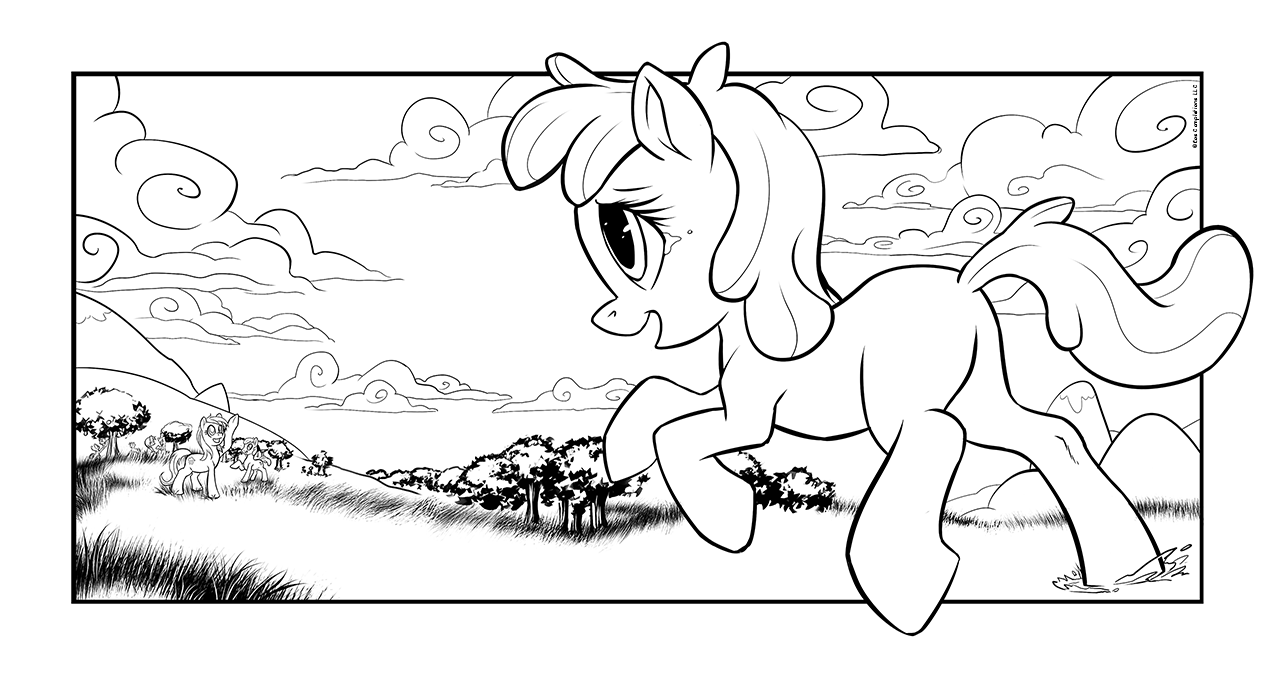
\includegraphics[width=0.9\linewidth]{image22.png}

\begin{motto}
    Do you believe in ghosts?

    你相信幽灵吗?
\end{motto}






\end{document}

